\documentclass{book} 
\usepackage{amsmath,amsthm,amsfonts,float} 
\usepackage{graphicx} 
\usepackage{tikz}
\usetikzlibrary{shapes.geometric}
\numberwithin{equation}{section}

\newtheorem{alevel}{A-LEVEL TASK}
\newtheorem{blevel}{B-LEVEL TASK}
\newtheorem{clevel}{C-LEVEL TASK}
\newtheorem{dlevel}{D-LEVEL TASK}
\newtheorem{elevel}{E-LEVEL TASK}
\theoremstyle{definition}
\newtheorem{bigidea}{BIG IDEA}
\newcommand{\longdiv}{\smash{mkern-0.43mu\vstretch{1.31}{\hstretch{.7}{)}}\mkern-5.2mu\vstretch{1.31}{\hstretch{.7}{)}}}}

%%%%%%%%%%%%%%%%%%%%%%%%%%%%%%%%%%%%%%%%%%%%%%%%%%%%%%%%%


\begin{document}
\title{Learning Electrical Circuit Analysis}
\author{Mark Stewart}
\maketitle
\tableofcontents

\chapter{Networks}

Like humans are mammals, electric cicuits are networks. As such we can learn some important ideas about circuits by first thinking a little bit about networks. \par

We have another motive for studying other networks. Electric circuits involve quantities that are difficult to picture. In order to form a decent mental picture of how they work, it can be useful to make analogies with networks that are easier to picture.\par

\begin{figure}[H]
\begin{center}
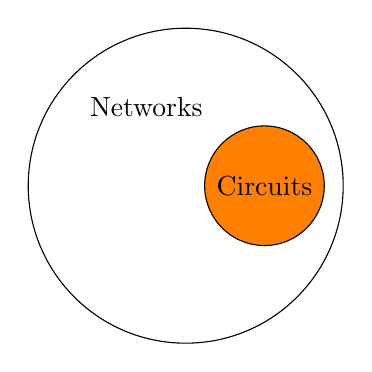
\begin{tikzpicture}
\node[draw,circle,minimum size =4cm] (A) at (0,0){};
\node[draw,circle,minimum size =1cm, fill=orange] (B) at (1,0){Circuits};
\node at (-.5,1) {Networks};
\end{tikzpicture}
\caption{Circuits are Networks}
\label{F:1FCAREN}
\end{center}
\end{figure}

In this first chapter, we take a tour of some other networks and with a mind on what we can apply to electrical networks (circuits). Starting in the next chapter, we'll devote ourselves more wholely to electric networks in particular.\par

\begin{bigidea} 
Electrical circuits are networks. They have a lot in common with other networks.
\end{bigidea}

\begin{bigidea} 
If you want to learn a specific, study the general. For example, if you want to learn about dogs, study mammals. See how dogs differ from racoons or kangaroos. 
\end{bigidea}

\section{Network Examples}

\subsection{A Network of Friends}
The diagram below shows a network of friends.

\begin{figure}[H]
\begin{center}
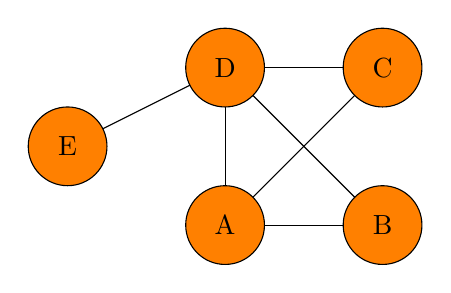
\begin{tikzpicture}
\draw (0,.5)--(0,1.5);
\draw (.5,2)--(1.5,2);
\draw (0,2)--(-2,1);
\draw (0,2)--(2,0);
\draw (0,0)--(2,0);
\draw (0,0)--(2,2);
\node[draw,circle,minimum size =1cm, fill=orange] (A) at (0,0){A};
\node[draw,circle,minimum size =1cm, fill=orange] (B) at (2,0){B};
\node[draw,circle,minimum size =1cm, fill=orange] (C) at (2,2){C};
\node[draw,circle,minimum size =1cm, fill=orange] (D) at (0,2){D};
\node[draw,circle,minimum size =1cm, fill=orange] (E) at (-2,1){E};
\end{tikzpicture}
\caption{A Friends Network}
\label{F:1FN}
\end{center}
\end{figure}

\par
\begin{alevel}
Who has the most friends?
\end{alevel}
\begin{alevel}
Draw a friend network that consists of 4 people where everybody has exactly two friends.
\end{alevel}
\par

\noindent
Networks have \textbf{nodes} and \textbf{edges}. The network in Figure~\ref{F:1FN} has 5 nodes. The edges connect nodes.  The meaning of the edges and node depends on the network. In our friend network, nodes represent people and edges represent relationships. For our friend network shown in Figure~\ref{F:1FN}, the edges have no direction to them. If A were friends with B, then B would be friends with A. However, this wouldn't have to be the case. We could add some directionality to the edges, like in the modified friends network shown in Figure~\ref{F:1FNb}:\\

\begin{figure}[H]
\begin{center}
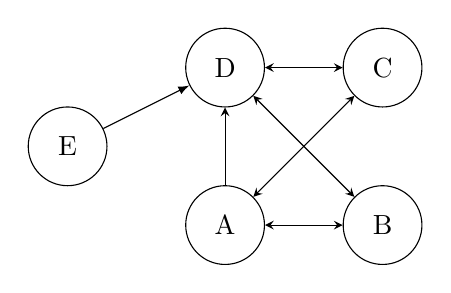
\begin{tikzpicture}
\node[draw,circle,minimum size =1cm] (A) at (0,0){A};
\node[draw,circle,minimum size =1cm] (B) at (2,0){B};
\node[draw,circle,minimum size =1cm] (C) at (2,2){C};
\node[draw,circle,minimum size =1cm] (D) at (0,2){D};
\node[draw,circle,minimum size =1cm] (E) at (-2,1){E};
\draw [stealth-stealth](A) edge (B);
\draw [stealth-stealth](C) edge (A);
\draw [-stealth](A) edge (D);
\draw [latex-](D) edge (E);
\draw [stealth-stealth](D) edge (C);
\draw [stealth-stealth](D) edge (B);
\end{tikzpicture}
\caption{Friends Network with Directional Edges}
\label{F:1FNb}
\end{center}
\end{figure}
\par

\noindent
If an arrow points only from A to B, then A is friends with B but that B is not friends with A. A bidirectional arrow means both people are friends with each other.\par

\begin{alevel}
How many people is D friends with?
\end{alevel}

\subsection{Road Networks}
Consider the road network shown in Figure~\ref{F:1RN} showing 5 towns connected together. The towns are called A, B, C, D and E. Each edge represents a road.\par
\begin{figure}[H]
\begin{center}
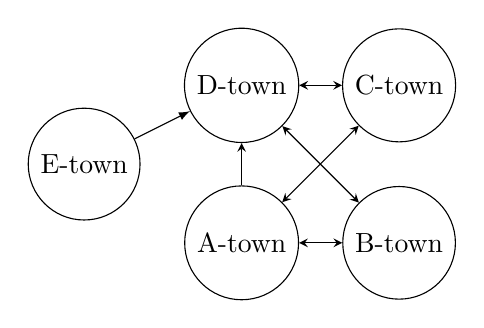
\begin{tikzpicture}
\node[draw,circle,minimum size =1cm] (A) at (0,0){A-town};
\node[draw,circle,minimum size =1cm] (B) at (2,0){B-town};
\node[draw,circle,minimum size =1cm] (C) at (2,2){C-town};
\node[draw,circle,minimum size =1cm] (D) at (0,2){D-town};
\node[draw,circle,minimum size =1cm] (E) at (-2,1){E-town};
\draw [stealth-stealth](A) edge (B);
\draw [stealth-stealth](C) edge (A);
\draw [-stealth](A) edge (D);
\draw [latex-](D) edge (E);
\draw [stealth-stealth](D) edge (C);
\draw [stealth-stealth](D) edge (B);
\end{tikzpicture}
\caption{Road Network}
\label{F:1RN}
\end{center}
\end{figure}

\begin{alevel}
For figure~\ref{F:1RN}, what does each node represent?
\end{alevel}

\begin{alevel}
How many roads are there?
\end{alevel}

\begin{alevel}
What does each edge represent?
\end{alevel}

\begin{alevel}
If each two-way road has two lanes and each one way road has one lane, how many lanes of road does the network have?
\end{alevel}

\begin{alevel}
If you start your trip at B-town, which town(s) can you not get to? If there are more than one, list them all.
\end{alevel}

\begin{clevel}
If you start your trip at E-town, is it possible to reach all the towns without traversing the same road twice? Does the answer to this question depend on the town where you start?
\end{clevel}

\begin{dlevel}
What would need to be true about ANY road network (all two way roads) such that you could always start at any town, travel some combination of roads, and reach every town without traversing any road twice?
\end{dlevel}

A road network diagram might convey more information. The edges could have a length (and/or width) associated with them. Figure~\ref{F:1RNb} shows a road network with the road length information added. 

\par
\begin{figure}[H]
\begin{center}
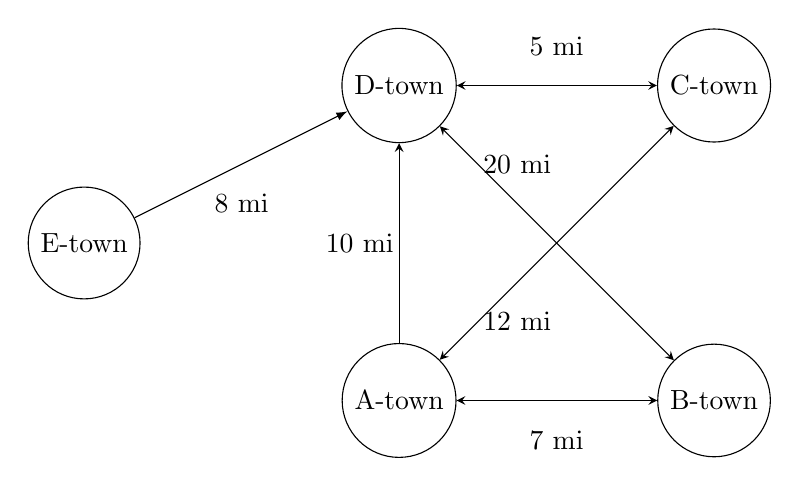
\begin{tikzpicture}
\node[draw,circle,minimum size =1cm] (A) at (0,0){A-town};
\node[draw,circle,minimum size =1cm] (B) at (4,0){B-town};
\node[draw,circle,minimum size =1cm] (C) at (4,4){C-town};
\node[draw,circle,minimum size =1cm] (D) at (0,4){D-town};
\node[draw,circle,minimum size =1cm] (E) at (-4,2){E-town};
\draw [stealth-stealth](A) edge (B);
\node at (2,-.5) {7 mi};
\draw [stealth-stealth](C) edge (A);
\node at (1.5,1) {12 mi};
\draw [-stealth](A) edge (D);
\node at (-.5,2) {10 mi};
\draw [latex-](D) edge (E);
\node at (-2,2.5) {8 mi};
\draw [stealth-stealth](D) edge (C);
\node at (2,4.5) {5 mi};
\draw [stealth-stealth](D) edge (B);
\node at (1.5,3) {20 mi};
\end{tikzpicture}
\caption{Road Network with edges that have values}
\label{F:1RNb}
\end{center}
\end{figure}

\begin{alevel}
What is the shortest distance to travel from E-Town to B-town?
\end{alevel}
\begin{alevel}
Name any node in this network.
\end{alevel}
\noindent
Now suppose there is some traffic on the network. \emph{Something} is flowing along the edges of the network - cars. Suppose there are:
\begin{enumerate}
\item 100 cars/minute flowing from E-town to D-town.  
\item 200 cars/minute (net) flowing from D-town to B-town
\item 50 cars/minute flowing from A-town to D-town
\item D-town and A-town and B-town have no parking at all, anywhere, zip, nada, none. If a town has no parking, the number of cars entering a town \textbf{must} equal the number of cars leaving.
\end{enumerate}

\begin{bigidea} 
Some networks are such that the \emph{flow} into a node must equal the \emph{flow} out of a node.
\end{bigidea}

\begin{alevel}
How many cars per minute must be driving along the road from B-town to A-town?
\end{alevel}

\begin{clevel}
How many cars per minute must be entering C-town?
\end{clevel}

\begin{dlevel}
Describe an algorithm to answer questions like the previous one.
\end{dlevel}

\noindent
Note that two of the roads seem to cross each other. Maybe they intersect there, maybe not. In this book, on a diagram, there is not an intersection unless the figure indicates one \footnote{Or unless it is obvious. Yikes! I realize this is disheartening because when you are new to something, very little seems obvious.}. A dot indicates an intersection, like in Figure~\ref{F:1RNb}.\par
\par
\begin{figure}[H]
\begin{center}
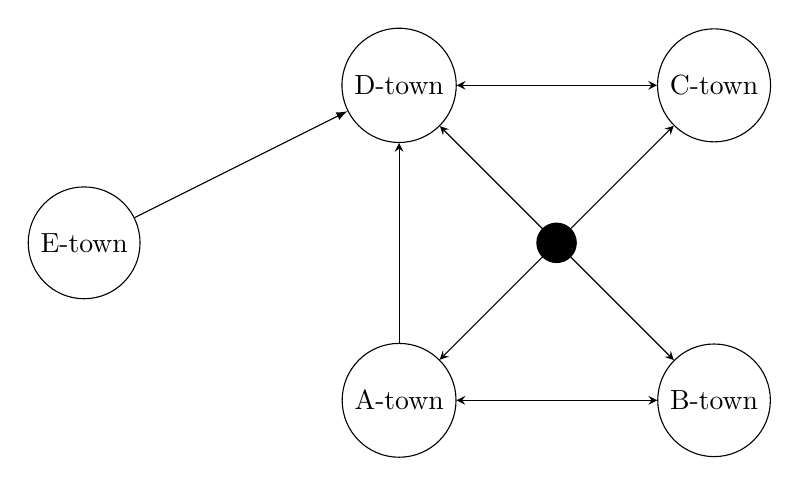
\begin{tikzpicture}
\node[draw,circle,minimum size =1cm] (A) at (0,0){A-town};
\node[draw,circle,minimum size =1cm] (B) at (4,0){B-town};
\node[draw,circle,minimum size =1cm] (C) at (4,4){C-town};
\node[draw,circle,minimum size =1cm] (D) at (0,4){D-town};
\node[draw,circle,minimum size =1cm] (E) at (-4,2){E-town};
\draw [stealth-stealth](A) edge (B);
\draw [stealth-stealth](C) edge (A);
\draw [-stealth](A) edge (D);
\draw [latex-](D) edge (E);
\draw [stealth-stealth](D) edge (C);
\draw [stealth-stealth](D) edge (B);
\node[draw, circle, minimum size=0.5cm, fill=black] at (2,2) {};
\end{tikzpicture}
\caption{Road network with an intersection indicated between Road AC and Road DB.}
\label{F:1RNb}
\end{center}
\end{figure}
\par

\subsection{Water Networks}
Consider the water network shown in Figure~\ref{F:1WN}.\\

\begin{figure}[H]
\begin{center}
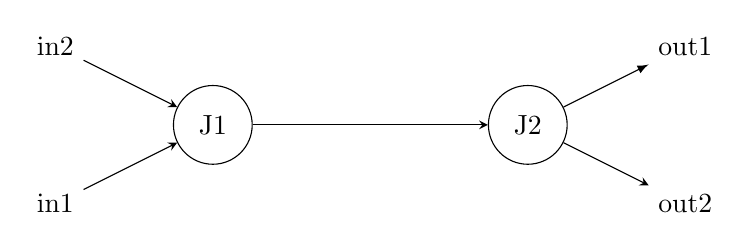
\begin{tikzpicture}
\node (In1) at (0,0){in1};
\node (In2) at (0,2){in2};
\node[draw,circle,minimum size =1cm] (J1) at (2,1){J1};
\node[draw,circle,minimum size =1cm] (J2) at (6,1){J2};
\node (Out1) at (8,2){out1};
\node (Out2) at (8,0){out2};
\draw [-stealth](In1) edge (J1);
\draw [-stealth](In2) edge (J1);
\draw [-stealth](J1) edge (J2);
\draw [-latex](J2) edge (Out1);
\draw [-stealth](J2) edge (Out2);
\end{tikzpicture}
\caption{Water Network}
\label{F:1WN}
\end{center}
\end{figure}

As with any network, you should begin by asking: What do the edges and nodes represent? For this water network\footnote{You might define things a little differently, but it doesn't matter here.}:
\begin{itemize}
\item Each of the \textbf{edges} represents a pipe or hose. Water flows along the edges.
\item Each of the \textbf{nodes} represents a junction, an input or an output. In1 and J2 are example of nodes.
\end{itemize}
What is flowing along the edges? Water.
How should we measure it? Hmmm. Maybe gallons per second (gps) or kg per second, or cubic meters per hour. Let's use gps.

\begin{blevel}
Ten gallons per second (gps) of water comes out the end of a hose. How many kg per second of water is this equivalent to?
\end{blevel}

\begin{blevel}
Suppose water flowed from in1 to J1 at 5 gps and in2 to J1 at 7 gps. Also suppose the flow from J1 to J2 were 10 gps. What would be happening to the amount of water stored in junction J1? How could this be?
\end{blevel}

\begin{clevel}
A 1cm radius water hose has some water flowing through it at a speed of 2 m/s. How many gallons per minute are flowing down this hose? Hint: Think about how much water passes a point in the hose each minute.
\end{clevel}

\subsection{A Neural Network}
Consider the neural network shown in Figure~\ref{F:1NN}. Each edge has a number (called a weight) associated with it. Each node is little calculator that combines the inputs and their weights to produce an output. For example, the calculation might be to sum the products of the inputs and their weights, and if that exceeds 5, then the output is 1, otherwise it is -1. 

The idea is that output depends on the input. By adjusting the weights this machine can be tuned to give a desired output, like "yes that is a piece of fruit" based on a set of inputs like the pixels in an image.
\begin{figure}[H]
\begin{center}
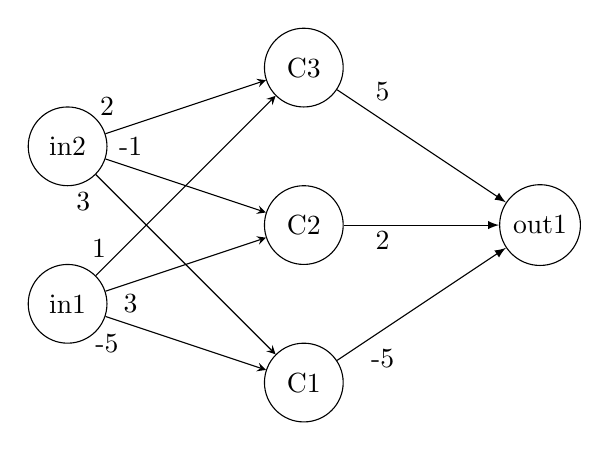
\begin{tikzpicture}
\node [draw,circle,minimum size =1cm](In1) at (0,0){in1};
\node [draw,circle,minimum size =1cm](In2) at (0,2){in2};
\node [draw,circle,minimum size =1cm](C1) at (3,-1){C1};
\node [draw,circle,minimum size =1cm](C2) at (3,1){C2};
\node [draw,circle,minimum size =1cm](C3) at (3,3){C3};
\node [draw,circle,minimum size =1cm](Out1) at (6,1){out1};
\draw [-stealth](In1) edge (C1);
\node at (.5,2.5) {2};
\draw [-stealth](In1) edge (C2);
\node at (.8,2) {-1};
\draw [-stealth](In1) edge (C3);
\node at (.2,1.3) {3};
\draw [-stealth](In2) edge (C1);
\node at (.4,0.7) {1};
\draw [-stealth](In2) edge (C2);
\node at (.8,0) {3};
\draw [-stealth](In2) edge (C3);
\node at (.5,-.5) {-5};
\draw [-latex](C1) edge (Out1);
\node at (4,2.7) {5};
\draw [-latex](C2) edge (Out1);
\node at (4,0.8) {2};
\draw [-latex](C3) edge (Out1);
\node at (4,-.7) {-5};
\end{tikzpicture}
\caption{A Neural Network}
\label{F:1NN}
\end{center}
\end{figure}

\begin{alevel}
For the neural network, what do the nodes represent?
\end{alevel}

\begin{blevel}
Suppose in1 were a 5 and in2 were a 10. What would be the output of C3? Hint: the output of C2 would be 1 because $-1*5+3*10 > 5$.
\end{blevel}

\begin{clevel}
If the output node contained the same calculating machines as the C-nodes, what would be the ouput if in1 were a 5 and in2 were a 10? 
\end{clevel}

\begin{clevel}
Let's call the product of the weight and the value on an edge the \em{flow}. Is it true that the flow into a node must equal the flow out of that node? 
\end{clevel}

\subsection{Summary}
In this section, we browsed some common networks. Let's see what we can takeaway:
\begin{itemize}
\item All networks have edges and nodes.
\item For some networks, the edges have values associated with them.
\item For some networks, the edges can be associated with a flow of something on them.
\item For some networks, the flow into a node must equal the flow out of a node. For other networks, this might not need to be the case.
\item A network might have a useful property, like all nodes have the same number of edges that touch them. Or all edge values are positive, or edges have a direction to them, or something else. Identifying such properties, if they exist, goes a long way towards understanding that particular network.
\end{itemize}




\chapter{Electrical Networks}
This chapter focuses on electrical circuits, a particular type of network. \footnote{We will often refer to an electrical network as a circuit.} Not surprisingly, circuit models contain nodes (junctions) and edges (wires or other components). The edges have values associated with them. And, we'll see that these networks obey certain rules.\par

\section{Electrical Charge}
Similar to road networks and water networks, something flows on the edges of electrical networks: electric charge. Unfortunately, though, moving electric charge can be harder to picture than driving cars or the flow of water.\par

\vspace{6pt}
\setlength{\hangindent}{30pt}\noindent
\textbf{Good Question:} What, exactly, is electrical charge? \par
\vspace{6pt}
\setlength{\hangindent}{30pt}\noindent
\textbf{Non-fullfilling Answer:} It is a property that some particles have. \par
\vspace{6pt}
\setlength{\hangindent}{30pt}\noindent
\textbf{Good Question:} But what's it made of? \par
\vspace{6pt}
\setlength{\hangindent}{30pt}\noindent
\textbf{Non-fullfilling Answer:} Sorry, but it might not be helpful to think of it as made of anything - it is just a property, like being symmetrical. However, so far, all particles with charge also have mass. Furthermore, and maybe surprisingly (or not\footnote{If charge weren't quantized then it would take an infinite amount of information to describe just the amount of charge on one ion. That really would be an odd universe. Take your pick which seems more odd to you.}) it comes in discrete chunks. We'll write ($1 e^-$) as the charge on 1 electron.

\begin{blevel}
Fill in the rest of Table~\ref{T:2EP}. Look stuff up online as needed.
\end{blevel}

\par
\begin{table}[H]
\begin{center}
\begin{tabular}{|c|c|} \hline
particle	&	charge (units of $e^-$) \\ \hline
electron	&	-1\\ \hline
proton		&	\\ \hline
top quark	&	\\ \hline
muon		&	\\ \hline
neutron		&	\\ \hline
photon		&	\\ \hline
Sodium Ion	&	\\ \hline
\end{tabular}
\caption{Summary of amount of charge that some particles have}
\label{T:2EP}
\end{center}
\end{table}

\begin{alevel}
What are the S.I. units of electrical charge?
\end{alevel}

\begin{blevel}
How many electrons would add up to one Coulomb of charge?
\end{blevel}

\subsection{Electrical Current}
Charge flows along the edges of electrical networks. We measure this flow in units of charge per time and we call (a flowrate of one Coulomb per one second) an (Ampere or Amp). Of course, $\frac{1}{10}$ of a Coulomb per $\frac{1}{10}$ second, would also equal one Amp of current during that time interval.
\par
\begin{alevel}
A wire carries a current of 5 Amps. How many Coulombs of charge pass through the wire each second? Each minute?
\end{alevel}

\begin{blevel}
A wire carries a current of 5 Amps. How many electrons pass through the wire each second? Each minute?
\end{blevel}

\begin{blevel}
Fill in table~\ref{F:2SU}.
\end{blevel}

\par
\begin{table}[H]
\begin{center}
\begin{tabular}{|c|c|c|c|} \hline
item	&	abbreviation & units & units abbreviation \\ \hline
Force	&	F	& Newton	& N\\ \hline
	&		&	&	kg	\\ \hline
charge	& q	&&	\\ \hline
current		&&&	\\ \hline
temperature		&&&	\\ \hline
Energy	&&&	\\ \hline
Power	&&&	\\ \hline
\end{tabular}
\caption{Symbols and units}
\label{F:2SU}
\end{center}
\end{table}

\noindent
The relationship between current, charge and time mirrors the relationship between acceleration, velocity and time. Electric current is the instantanous rate at which charge passes along an edge, just like acceleration is the instantaneous rate at which velocity is changing. \footnote{If anything, it is simpler because we don't need to worry about current or charge being vectors, at least not in this context.} 

\par
\begin{align}
\vec{a} = \frac{d\vec{v}}{dt}&&\leftrightarrow&&I = \frac{dq}{dt}
\end{align}
\par
Figure~\ref{F:2CAR} shows the velocity of a car as a function of time.
\par
\begin{figure}[H]
\begin{center}
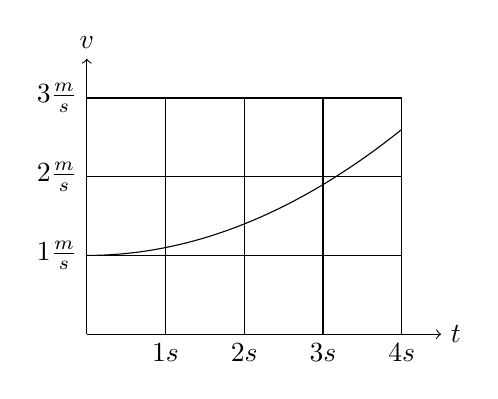
\begin{tikzpicture}
\draw[->] (0,0)--(4.5,0) node[right] {$t$};
\draw[->] (0,0)--(0,3.5) node[above] {$v$};
\draw (0,1)node[left] {$1 \frac{m}{s}$} --(4,1);
\draw (0,2)node[left] {$2 \frac{m}{s}$}--(4,2) ;
\draw (0,3)node[left] {$3 \frac{m}{s}$}--(4,3) ;
\draw (1,0)node[below] {$1 s$}--(1,3) ;
\draw (2,0)node[below] {$2 s$}--(2,3) ;
\draw (3,0)node[below] {$3 s$}--(3,3) ;
\draw (4,0)node[below] {$4 s$}--(4,3) ;
\draw [smooth, samples=100,domain=0:4] plot(\x,{.1*(\x)*(\x)+1});
\end{tikzpicture}
\caption{A car's velocity as a function of time.}
\label{F:2CAR}
\end{center}
\end{figure}

\begin{alevel}
How fast is the car going at 4 seconds?
\end{alevel}

\begin{blevel}
Trick question: What is the position of the car after 1 s?
\end{blevel}

\begin{dlevel}
Why was the previous question a trick question? What piece of information was missing?
\end{dlevel}

\begin{blevel}
What is the average acceleration of the car between 0 and 4 seconds?
\end{blevel}

\begin{blevel}
What is the instantaneous acceleration of the car when the time is 0 seconds? Hint: acceleration is the slope of a v-t graph.
\end{blevel}

\begin{blevel}
What is the instantaneous acceleration of the car at a time of 4 seconds?
\end{blevel}
\begin{clevel}
Sketch the car's acceleration between t=0 and t=4 s. Label your axes.
\end{clevel}
\noindent
Consider the graph in Figure~\ref{F:2QT} which shows the charge at some node as a function of time.
\par
\begin{figure}[H]
\begin{center}
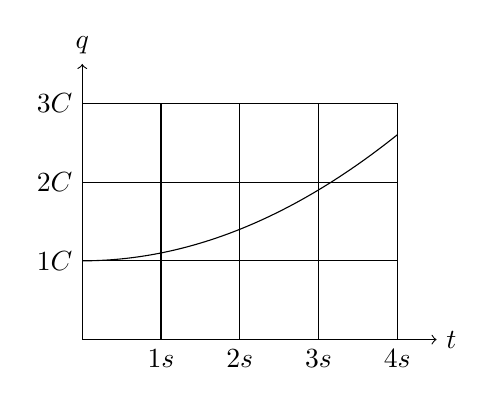
\begin{tikzpicture}
\draw[->] (0,0)--(4.5,0) node[right] {$t$};
\draw[->] (0,0)--(0,3.5) node[above] {$q$};
\draw (0,1)node[left] {$1 C$} --(4,1);
\draw (0,2)node[left] {$2 C$}--(4,2) ;
\draw (0,3)node[left] {$3 C$}--(4,3) ;
\draw (1,0)node[below] {$1 s$}--(1,3) ;
\draw (2,0)node[below] {$2 s$}--(2,3) ;
\draw (3,0)node[below] {$3 s$}--(3,3) ;
\draw (4,0)node[below] {$4 s$}--(4,3) ;
\draw [smooth, samples=100,domain=0:4] plot(\x,{.1*(\x)*(\x)+1});
\end{tikzpicture}
\caption{Charge as a function of time.}
\label{F:2QT}
\end{center}
\end{figure}

\begin{alevel}
How much charge is on the node after 4 seconds?
\end{alevel}
\begin{blevel}
What is the average current into the node between 0 and 4 seconds?
\end{blevel}
\begin{blevel}
What is the instantaneous current into the node at a time of 4 seconds?
\end{blevel}
\begin{clevel}
Graph the current into the node, I(t), between t=0 and t=4 s.
\end{clevel}

\begin{alevel}
A node has a net current entering it of $i=(3q+1)$ Amps. What are the units of the '3'?
\end{alevel}

\begin{clevel}
A node has a net current entering it of $i=(3q+1)$ Amps. The initial amount of charge at the node  is 5 C. Determine the amount of charge present at the node as a function of time.
\end{clevel}

\begin{clevel}
A node has a net charge on it of $q=(3e^{2t}+1)$ Coulombs. Determine the current onto this node as a function of time.
\end{clevel}

%%%%%%%%%%%%%%%%%%%%%%%%%%%%%%%%%%%%%%%%%%%%%%%%%%%%%%%%%
\section{Voltage}
Like electrical current, voltage is also a special quantity in analyzing electrical networks. This section deals with learning what voltage is and how it might be useful.\par

A voltage difference represents an electrical energy difference per amount of charge. That takes a little time to unpack. Let's start with reviewing what we mean by energy.

\subsection{Energy}
We need energy to do anything. An object that speeds up gains kinetic energy. It takes work (a transfer of energy) to drag something across the floor. It takes energy to create mass and, likewise, mass can be converted back into energy (atomic bombs). In this class, we are particularly concerned with the electrical energy needed to squish charges together.
\par
\begin{clevel}
Fill in the rest of this table. Look up formulae as needed.
\end{clevel}

\begin{table}[H]
\begin{center}
\begin{tabular}{|c| c| c|} \hline
item & relevant formula	& rough value \\ \hline
stand up	& W = F*d	& $(100kg)*(9.8 \frac{m}{s^2})*.5 m \approx 500J$\\ \hline
heat up cup of coffee &	& \\ \hline
start running sideways	&	&\\ \hline
drag a log 20 feet	&	&\\ \hline
create a 1kg of mass	&	&\\ \hline
create one photon ($\lambda$=650 nm)	&	&	\\ \hline
case A*			&	&\\ \hline
case B*			&	&\\ \hline
\end{tabular}
\caption{Approximate amount of energy needed to do several tasks.}
\end{center}
\end{table}

\noindent
*case A: Move two electrons from a distance of 4 m apart to a distance of 2 m apart.
\par
\noindent
*case B: Separate two 1kg masses that are initially 2m apart to make them 4 m apart\footnote{The gravitational potential energy is for the system, not just one of the masses by itself}.
\linebreak

\begin{blevel}
What is the principle of conservation of energy?
\end{blevel}

\par
To understand voltage, it might be useful to begin by studying its gravitational counterpart, gravitational potential energy per mass. Figure~\ref{F:2MT} shows a mountain with a hiking trail network starting at the parking lot labeled P:
\par
\begin{figure}[H]
\begin{center}
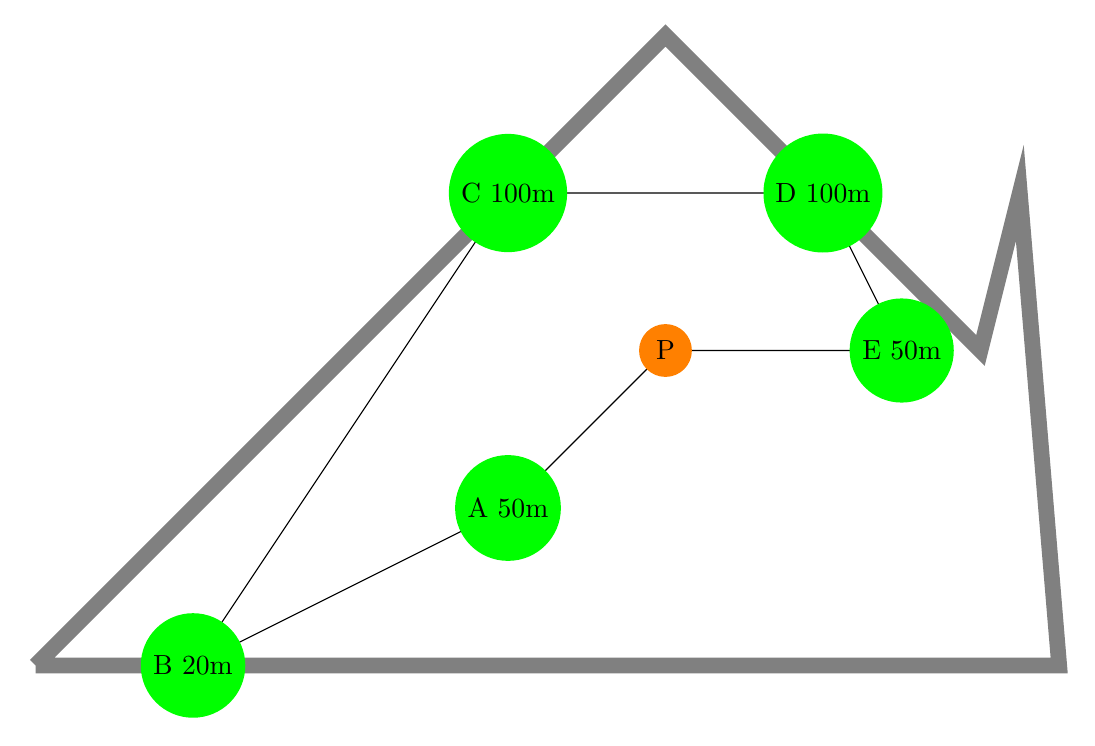
\begin{tikzpicture}
\draw [draw=gray, line width=2mm] (0,0)--(8,8)--(12,4)--(12.5,6)--(13,0)--(0,0);
\draw (8,4) node[circle, radius=0.25cm, fill=orange] {P}
--(6,2) node[circle, radius=0.25cm, fill=green] {A 50m}
--(2,0) node[circle, radius=0.25cm, fill=green] {B 20m}
--(6,6) node[circle, radius=0.25cm, fill=green] {C 100m}
--(10,6) node[circle, radius=0.25cm, fill=green] {D 100m}
--(11,4) node[circle, radius=0.25cm, fill=green] {E 50m} -- cycle;
\end{tikzpicture}
\caption{A mountain with a parking lot, P and a trail system. The labels indicate the heights of those points above some reference point.}
\label{F:2MT}
\end{center}
\end{figure}

\begin{alevel}
What do the edges in the network represent?
\end{alevel}
\begin{blevel}
Do the nodes in the network have a number associated with them? What is it?
\end{blevel}
\begin{alevel}
What is the total change in height when hiking from the parking lot, around the trail, and back to the parking lot?
\end{alevel}
\begin{blevel}
Generalize your answer to the above question.
\end{blevel}
\begin{blevel}
Suppose a 50 kg hiker named Comet and an 80kg hiker named Ajax start at the parking lot and hike to point D. What are the respective changes in gravitational potential energy for the Comet-Earth system and the Ajax-Earth system? What are the corresponding gains in gravitational potential energy per mass?
\end{blevel}

Tracking changes in (gravitational potential energy per mass) can be useful because these changes only depend on the shape of the trail, not who is hiking it. Scientists shorten (gravitational potential energy per mass) to (gravitational potential) and give it the symbol V (I'll use $V_G$ so as not to confuse it with Voltage, V).
\begin{align}
V_G=\frac{PE_{GRAV}}{m}&&\text{Gravitational Potential} \label{E:2GP}
\end{align}

Let's write the gravitational potential difference from A to B as $V_{AB}$. If pt. B represents a higher grav. potential than A, this would be positive. Note that: $V_{AB}=-V_{BA}$.

\begin{blevel}
Use the above mountain trail graphic to fill in Table~\ref{T:2GP}.
\end{blevel}

\begin{table}[H]
\begin{center}
\begin{tabular}{|c|c|}\hline
pts&Grav. Potential ($V_G$)\\ \hline
$V_{AB}$& \\ \hline
$V_{AC}$& \\ \hline
$V_{CE}$& \\ \hline
$V_{CD}$& \\ \hline
$V_{EC}$& \\ \hline
\end{tabular}
\caption{Values for gravitational potential energy per mass (gravitational potential)}
\label{T:2GP}
\end{center}
\end{table}

\begin{clevel}
Does gravitation potential flow?
\end{clevel}

\begin{blevel}
What are the units of gravitational potential?
\end{blevel}

\subsection{Voltage - finally}
Instead of gravitational energy per mass, we'll be using its electrical equivalent, electrical energy per charge. Some people call it the electric potential, but in the context of electrical networks, we usually say Voltage. \par

Consider Figure~\ref{F:2Va}. If it takes 5 Joules of energy to move +2 Coulombs of charge from pt A to pt B, then we would say there is a 2.5 Volt difference between pts A and B.

\begin{figure}[H]
\begin{center}
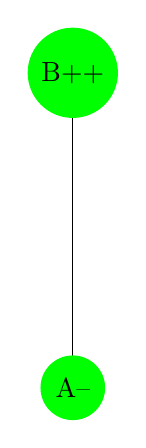
\begin{tikzpicture}
\draw (2,0) node[circle, radius=0.25cm, fill=green] {A--}
--(2,4) node[circle, radius=0.25cm, fill=green] {B++};
\end{tikzpicture}
\caption{Two nodes. A has some negative charge and B has some positive charge.}
\label{F:2Va}
\end{center}
\end{figure}

The reason it would require energy (effort) to move charge from A to B is because B is positively charged, and the +2C charge would repel node B.
\par
\begin{blevel}
How much energy would it take to move 9C of charge from A to B?
\end{blevel}

\begin{alevel}
Does voltage flow?
\end{alevel}

\begin{blevel}
What is the electrical equivalent for Equation~\eqref{E:2GP}?
\end{blevel}

%%%%%%%%%%%%%%%%%%%%%%%%%%%%%%%%%
\subsection{Power}
Power is the rate at which energy is being transformed from one form to another. We (even scientists) might say consumed or produced, but we don't really mean it. The total enery in a closed system stays the same. You can't \emph{use up} energy. We're not producing energy, but rather transforming it from one form to another. The sun does not produce energy, it transforms it from mass energy into photons.
\par
\begin{alevel}
Does a power plant actually produce energy?
\end{alevel}

\begin{alevel}
(Energy per gallon) times (gallons per second). What units does this give?
\end{alevel}

\begin{blevel}
A 300W blender is in use for 25 seconds. How much energy does this use?
\end{blevel}

\begin{clevel}
A car gets 25 mpg. It travels 50 miles at a speed of 60 mph. At what rate (in Watts) is the car using its gas? Hint: How much time did it take to go 60 miles?
\end{clevel}

\begin{alevel}
How many Watts are equivalent to 1 horsepower?
\end{alevel}

\noindent\fbox{\parbox{\textwidth}{
\textbf{Example Power Calculation:}\par
Suppose water flows over a 4-meter tall water-wheel at a rate of 10 gallons per second. Estimate the rate at which the water wheel system can \emph{produce}\footnote{Again, we're really just transforming it from one form to another} power (assuming 100\% efficiency). Let's break this problem into a couple steps.

\par
\begin{itemize}
\item \textbf{Step 1:} Determine the gravitational potential energy difference per gallon of water. It will be the gravitational potential energy difference of the gallon being at the top of the water wheel verses at the bottom. Gravitional potential energy is mgh, or:
\begin{align*}
PE&=mgh\\
PE &= \rho (Volume)gh\\
\frac{PE}{V}&=\rho gh &\leftarrow&\text{potential energy per volume}\\
\frac{PE}{V}&= 1000*9.8*4 \approx 40000 \frac{J}{m^3}
\end{align*} 

Just convert this to gallons and we're done with this part.
\item \textbf{Step 2:} Recall that power is energy per time. We know energy per gallon. To convert to energy per time (power), multiply energy per gallon by gallons per second (given).
\end{itemize}

\begin{blevel}
What is the difference in $V_G$ between the bottom and top of the water wheel?
\end{blevel}

\begin{blevel}
Finish the above water wheel problem with the numbers given. Determine the power produced by the water wheel.
\end{blevel}

}}


\begin{blevel}
Justify the equation P=IV based on units. Hint: What are the units of current? What are the units of voltage (don't say Volts)?
\end{blevel}

\begin{clevel}
A well pump pushes water up from a depth of 200 feet. How much power is needed (in Watts) if the pump is to pump 10 gallons/minute?
\end{clevel}

\begin{clevel}
A 1000 kg car drives up a $5^0$ hill at 5 m/s. Ignore air drag. Determine the power needed from the engine.
\end{clevel}

\begin{blevel}
A resistor has a voltage difference across it of 5V and a current through it of 6Amps. How many Joules of energy does it dissipate each minute?
\end{blevel}

%%%%%%%%%%%%%%%%%%%%%%%%%%%%%%%%%%%%%%%%%%%%%%%%%%%%%%%%%%

\subsection{Application: Solar Cells}
Sunlight, like all light, is made of lots of individual packets of light called photons. Photons are interesting little particles in their own right. \footnote{For one thing, because they travel at the speed of light, time does not pass for a photon from its point of view. A photon is created and absorbed, potentially on the other side of the universe, at the same instant.}\par

Each photon transfers a small chunk of energy. Depending on how many photons are being absorbed and how much enery each one has, one can determine how much power is being transferred by light. At the Earth's surface, sunlight transfers about $1000 \frac{W}{m^2}$. Modern solar cells can capture about a quarter of this power.

A typical solar panel might produce 300 Watts in full sun\footnote{In 2021}.

\begin{alevel}
What is a particle of light called?
\end{alevel}
\begin{blevel}
How big (area) would a 300W solar panel need to be if it were 19\% efficient?
\end{blevel}
\begin{blevel}
If this panel were left out in the sun for 3 hours, how much energy would it collect?
\end{blevel}
\begin{blevel}
If this panel produced 48V, and were connected to a load designed to draw max power, how much current would it produce (still in full sun)?
\end{blevel}
\begin{blevel}
How many of these panels would be needed to generate 150 hp?
\end{blevel}

Consider the following two arrangements of ways to connect two solar panels. In both cases the individual panels produce 300W at a voltage of 48V.
\par

\begin{figure}[H]
\begin{center}
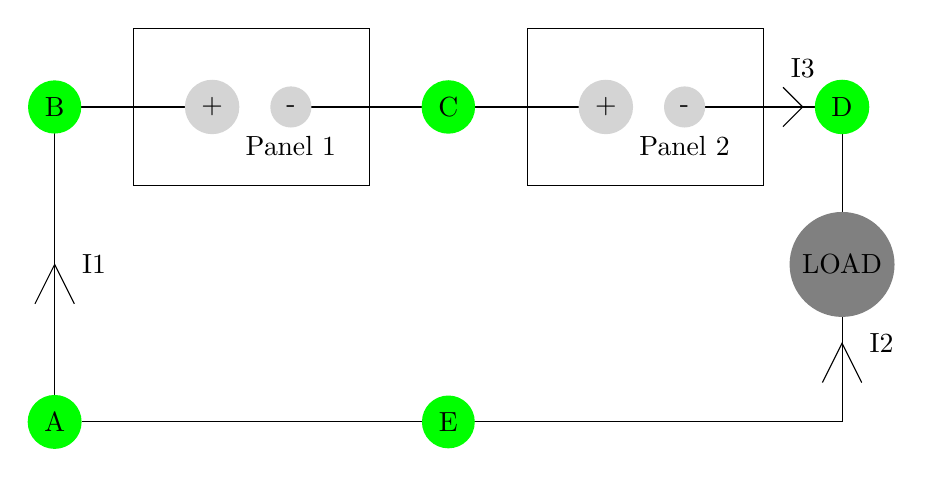
\begin{tikzpicture}
\draw (0,0) node[circle, radius=0.25cm, fill=green] (A) {A}
--(0,4) node[circle, radius=0.25cm, fill=green] {B}
--(2,4) node[circle, radius=0.1cm, fill={rgb:black,1;white,5}] {+};
\draw (3,4) node[circle, radius=0.1cm, fill={rgb:black,1;white,5}] {-}
--(5,4) node[circle, radius=0.25cm, fill=green] {C}
--(7,4) node[circle, radius=0.1cm, fill={rgb:black,1;white,5}] {+};
\draw (8,4) node[circle, radius=0.1cm, fill={rgb:black,1;white,5}] {-}
--(10,4) node[circle, radius=0.25cm, fill=green] {D}
--(10,2) node[circle, radius=0.1cm, fill={rgb:black,1;white,1}] {LOAD}
--(10,0)
--(5,0) node[circle, radius=0.25cm, fill=green] {E}
--(A);
\draw [draw=black] (1,3) rectangle (4,5);
\draw [draw=black] (6,3) rectangle (9,5);
\node at (3,3.5) {Panel 1};
\node at (8,3.5) {Panel 2};
\draw (-.25,1.5)--(0,2)--(.25,1.5) (.5,2) node{I1};
\draw (9.75,.5)--(10,1)--(10.25,.5) (10.5,1) node{I2};
\draw (9.25,3.75)--(9.5,4)--(9.25,4.25) (9.5,4.5) node{I3};
\end{tikzpicture}
\caption{Arrangment 1.}
\end{center}
\end{figure}

\begin{figure}[H]
\begin{center}
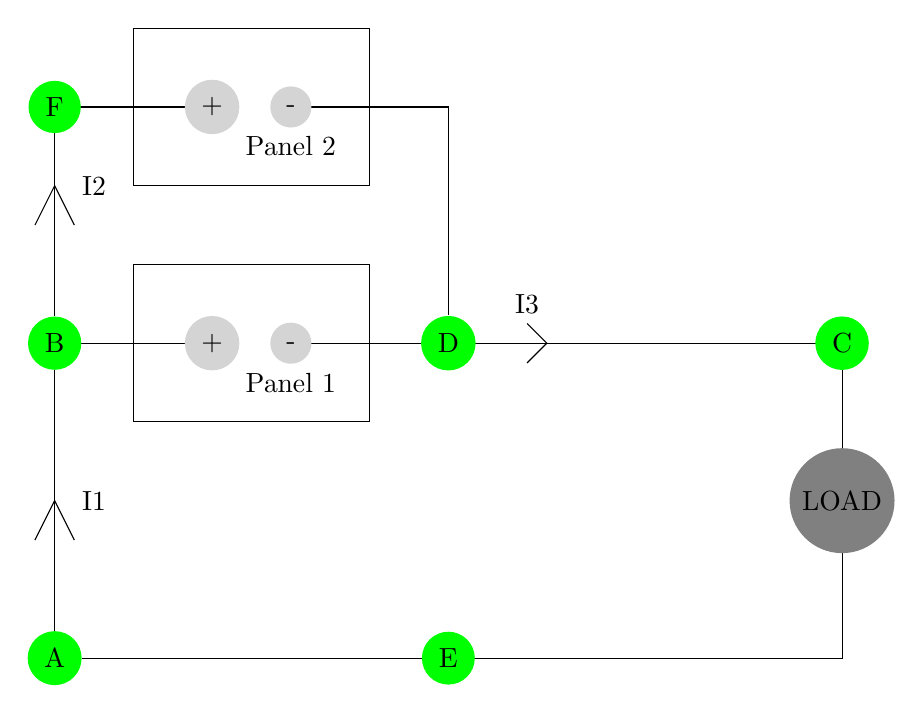
\begin{tikzpicture}
\draw (0,0) node[circle, radius=0.25cm, fill=green] (A) {A}
--(0,4) node[circle, radius=0.25cm, fill=green] (B) {B}
--(2,4) node[circle, radius=0.1cm, fill={rgb:black,1;white,5}] {+}
(3,4) node[circle, radius=0.1cm, fill={rgb:black,1;white,5}] {-}
--(5,4) node[circle, radius=0.25cm, fill=green] (D) {D}
--(10,4) node[circle, radius=0.25cm, fill=green] {C}
--(10,2) node[circle, radius=0.1cm, fill={rgb:black,1;white,1}] {LOAD}
--(10,0)
--(5,0) node[circle, radius=0.25cm, fill=green] {E}
--(A);
\draw (B)--(0,7) node[circle, radius=0.25cm, fill=green] {F}
--(2,7) node[circle, radius=0.1cm, fill={rgb:black,1;white,5}] {+}
(3,7) node[circle, radius=0.1cm, fill={rgb:black,1;white,5}] {-}
--(5,7)--(D);
\draw [draw=black] (1,3) rectangle (4,5);
\draw [draw=black] (1,6) rectangle (4,8);
\node at (3,3.5) {Panel 1};
\node at (3,6.5) {Panel 2};
\draw (-.25,1.5)--(0,2)--(.25,1.5) (.5,2) node{I1};
\draw (-.25,5.5)--(0,6)--(.25,5.5) (.5,6) node{I2};
\draw (6,3.75)--(6.25,4)--(6,4.25) (6,4.5) node{I3};
\end{tikzpicture}
\caption{Arrangment 2.}
\end{center}
\end{figure}

\begin{blevel}
Fill in the following table.
\end{blevel}
\par
\begin{table}[H]
\begin{center}
\begin{tabular}{|c|c|c|}\hline
which points	& Voltage (Arrangement 1)&Voltage (Arrangement 2) \\ \hline
BC & & \\ \hline
CB & & \\ \hline
AB & & \\ \hline
BD & & \\ \hline
DE & & \\ \hline
DA & & \\ \hline
AD & & \\ \hline
FD & n/a & \\ \hline	
\end{tabular}
\end{center}
\end{table}

\begin{blevel}
For any arrangement, how much current must be flowing through Panel 1 and Panel 2 in order for them to each produce 300W of power? Note: Since the panel is producing power, the current would flow from the negative side to the positive side.
\end{blevel}

Note the arrows labeled on some of the wires. These arrows indicate the current passing through those wires.
\par
\begin{blevel}
Fill in the currents indicated in Table~\ref{T:2SSC}.
\end{blevel}

\par
\begin{table}[H]
\begin{center}
\begin{tabular}{|c|c|c|}\hline
which current	& Current (Arrangement 1)&Current (Arrangement 2) \\ \hline
I1 & & \\ \hline
I2 & & \\ \hline
I3 & & \\ \hline
\end{tabular}
\label{T:2SSC}
\end{center}
\end{table}

\begin{blevel}
Determine the voltage difference across the load and the current through the load for both arrangements. For each case, calculate the power absorbed by the load.
\end{blevel}

\begin{clevel}
Design, using 100W, 20V panels an arrangment of panels that produces 40V at the load and 800W of power.
\end{clevel}

%%%%%%%%%%%%%%%%%%%%%%%%%%%%%%%%%%%%%%%%%%%%%%%%%%%%%%%%%%%
\subsection{Application: Electric cars}
Electric cars store energy and convert that energy into motion when you drive.\par

A gallon of gas stores about 100 Million Joules of energy. (Great Scott! That's a lot of energy.) Diesel fuel stores a little more energy per gallon than regular unleaded gas. Electric cars store the energy in a electrical battery\footnote{How the energy is stored isn't really what makes it an electric car. A fun conversation could be had on what exactly an electric car needs to have in order to be called an electric car.}. Alternatively, one could store the energy as gas, then use it to charge a battery, then use the battery to power the motor\footnote{It's up to you as whether or not you'd still call it an electric car}.

\begin{figure}[H]
\begin{center}
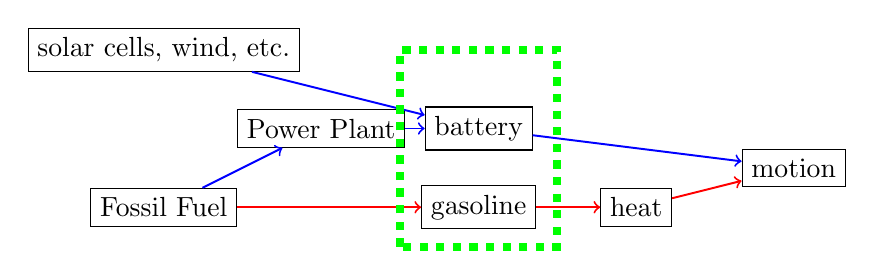
\begin{tikzpicture}
\draw (0,0) node[draw=black, radius=.25 cm, fill=white](G){gasoline}
(2,0) node[draw=black, radius=.25 cm, fill=white](H){heat}
(4,.5) node[draw=black, radius=.25 cm, fill=white](M){motion};
\draw [draw=red, line width=0.25mm] [->] (G)--(H);
\draw [draw=red, line width=0.25mm] [->] (H)--(M);
\draw (-2,1) node[draw=black, radius=.25 cm, fill=white](PP){Power Plant}
(-4,2) node[draw=black, radius=.25 cm, fill=white](SS){solar cells, wind, etc.}
(0,1) node[draw=black, radius=.25 cm, fill=white](B){battery}
(-4,0) node[draw=black, radius=.25 cm, fill=white](FF){Fossil Fuel};
\draw [draw=blue, line width=0.25mm] [->] (B)--(M);
\draw [draw=blue, line width=0.25mm] [->] (SS)--(B);
\draw [draw=blue, line width=0.25mm] [->] (PP)--(B);
\draw [draw=red, line width=0.25mm] [->] (FF)--(G);
\draw [draw=blue, line width=0.25mm] [->] (FF)--(PP);
\draw [draw=green, line width=1 mm, dashed] (-1,-.5)--(-1,2)--(1,2)--(1,-.5)--(-1,-.5);
\end{tikzpicture}
\caption{Energy transfer chains for electric cars (blue) and gas cars (red). The dashed box represents the energy storage options for the car.}
\end{center}
\end{figure}

We quantify the amount of amount of energy stored in a battery with a variety of units. One could certainly use Joules, but many times people use a common alternative called the kilo-Watt-hour. One kWr stores the equivalent amount of energy as using 1000 Watts for one hour.

\begin{alevel}
If someone uses 10 Watts for 20 seconds, how much energy did they use?
\end{alevel}

\begin{blevel}
Someone says they have a solar panel that produces 500W per day. Why is this a confusing statement?
\end{blevel}

\begin{blevel}
How many Joules are equivalent to 1 kW-hr?
\end{blevel}

\begin{blevel}
A 300W solar panel sits out in direct sun for 5 hours. How many kWhr of energy does it collect?
\end{blevel}

\begin{blevel}
How many kWhr are equivalent to 1 gallon of gas? \footnote{This is a little misleading because the gas will be burned to produce thermal energy and then that thermal energy is transformed into kinetic energy. The process is less efficient than the direct conversion of chemical potential energy stored in a battery into the motion of the car. In order words, at least for cars, 1 kWhr or battery storage is more valuable than 1 kWhr of gas.}
\end{blevel}

When buying electricity through the grid, you will probably pay per kWhr, the cost of which is around 20 cents in NY (year 2021)\footnote{Delivered, including transport costs, not just generation}.

\begin{blevel}
The 2021 Chevvy Bolt has a battery size of 65kWhrs. How many Joules does this battery store? If someone comes to your house and needs to charge their entire car battery through your garage plug, how much will this cost you? 
\end{blevel}

\begin{blevel}
You plug your electric car into a normal wall outlet to charge up. The wall outlet can not draw more than 10A without tripping a breaker and has a voltage of 120V. Determine the max power that can be drawn from the outlet to charge the car. At this max power, how much time will it take to charge the car battery? Assume the battery starts as a dead battery. 
\end{blevel}

\begin{blevel}
Special chargers have been constructed that can draw much more power than your wall outlet can provide. These chargers can deliver more like 200,000 Watts. How much time will these super chargers take to charge up an electric car like the Chevvy Bolt?
\end{blevel}


%%%%%%%%%%%%%%%%%%%%%%%%%%%%%%%%%%%%%%%%%%%%%%%%%%%%%%%%%%%
\section{Network Summary Table}

\begin{blevel}
Fill in this table.
\end{blevel}

\par
\begin{table}[H]
\begin{center}
\begin{tabular}{ |c | c | c | c |} \hline
network	&	what are nodes	& what are edges	& what flows \\ \hline
friends	&	people	& indications of friendship	& n/a \\ \hline
traffic &		&				&	\\ \hline
water	&		&				&	\\ \hline
electrical	& places of equal electrical energy	&	&	\\ \hline
\end{tabular}
\caption{Network Summary Table}
\end{center}
\end{table}

%%%%%%%%%%%%%%%%%%%%%%%%%%%%%%%%%%%%%%%%%%%%%%%%%%%%%%%%%%%%%%%%%%%%%%%%%%%%%%%%%
\section{An Important Summary Diagram: The Six Circles.}
This chapter covered some of quantities relevant to electrical networks, like energy, voltage, charge, and current. Eventually, you may also need to keep straight electric fields, gravitational fields, forces and work. Table~\ref{F:26C} summarizes the relationships between some of these parameters and may help place voltage and force in a larger context.
\par
Start with the relationship between force and potential energy. Dividing these quantities by mass results in the gravitational field and gravitational potential. Divide by charge instead leads to electric field and voltage. Use the same relationships to move left-right or uo-down on the diagram. Knowing these relationships means you actually know all 14 equations!
\par
\begin{figure}[H]
\begin{center}
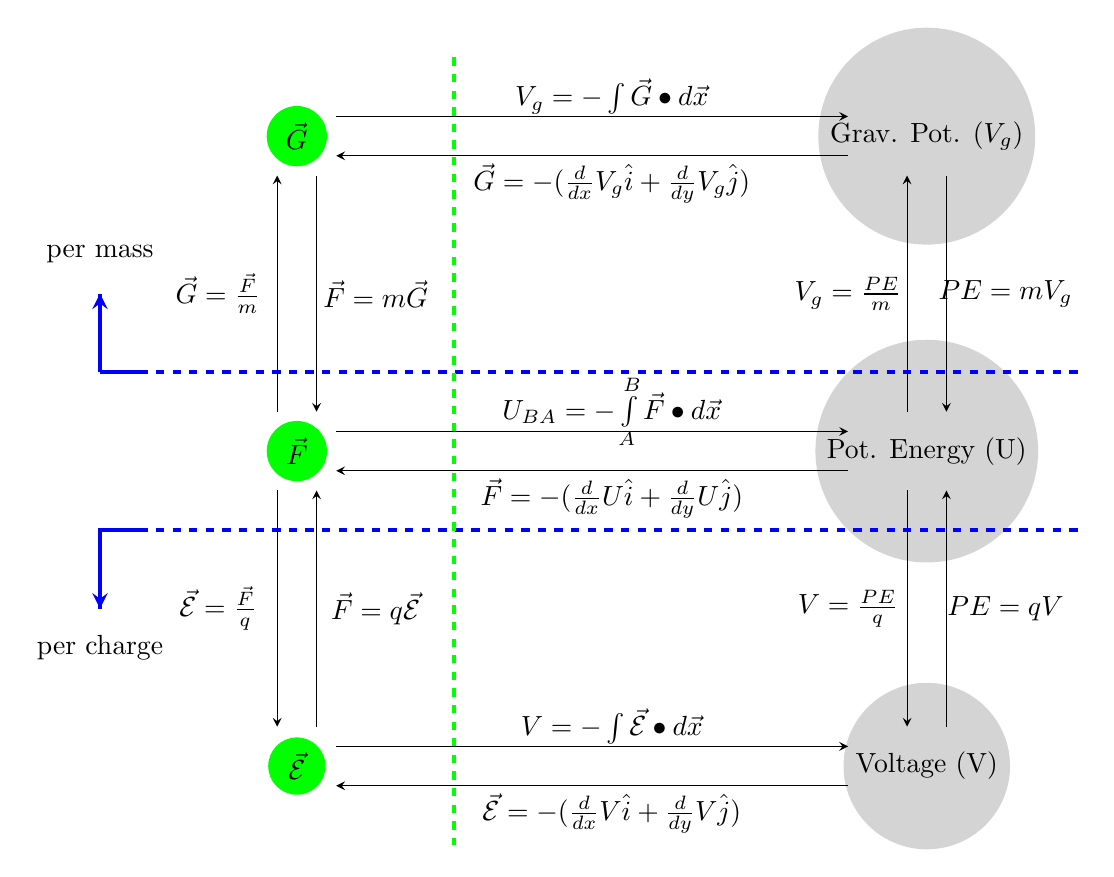
\begin{tikzpicture}
\draw (0,0) node[circle, radius=0.25cm, fill=green] (F) {$\vec{F}$}
(0,4) node[circle, radius=0.25cm, fill=green] (G) {$\vec{G}$}
(8,4) node[circle, radius=0.25cm, fill={rgb:black,1;white,5}] {Grav. Pot. ($V_g$)}
(8,0) node[circle, radius=0.1cm, fill={rgb:black,1;white,5}] (E) {Pot. Energy (U)}
(0,-4) node[circle, radius=0.25cm, fill=green] (Ef) {$\vec{\mathcal{E}}$}
(8,-4) node[circle, radius=0.25cm, fill={rgb:black,1;white,5}] {Voltage (V)};
%vertical
\draw [-stealth](-.25,.5)--(-.25,3.5);
\draw [stealth-](.25,.5)--(.25,3.5);
\draw node at (-1,2) {$\vec{G} = \frac{\vec{F}}{m}$};
\draw node at (1,2) {$\vec{F} = m\vec{G}$};
\draw [-stealth](7.75,.5)--(7.75,3.5);
\draw [stealth-](8.25,.5)--(8.25,3.5);
\draw node at (7,2) {$V_g = \frac{PE}{m}$};
\draw node at (9,2) {$PE = mV_g$};
\draw [-stealth](-.25,-.5)--(-.25,-3.5);
\draw [stealth-](.25,-.5)--(.25,-3.5);
\draw node at (-1,-2) {$\vec{\mathcal{E}} = \frac{\vec{F}}{q}$};
\draw node at (1,-2) {$\vec{F} = q\vec{\mathcal{E}}$};
\draw [-stealth](7.75,-.5)--(7.75,-3.5);
\draw [stealth-](8.25,-.5)--(8.25,-3.5);
\draw node at (7,-2) {$V = \frac{PE}{q}$};
\draw node at (9,-2) {$PE = qV$};
%horizontal
\draw [-stealth] (.5,.25)--(7,.25);
\draw [stealth-] (.5,-.25)--(7,-.25);
\draw node at (4,.5) {$U_{BA} = -\int\limits_A^B{\vec{F}\bullet d\vec{x}}$};
\draw node at (4,-.6) {$\vec{F} = -(\frac{d}{dx}U\hat{i}+\frac{d}{dy}U\hat{j})$};
\draw [-stealth] (.5,4.25)--(7,4.25);
\draw [stealth-] (.5,3.75)--(7,3.75);
\draw node at (4,4.5) {$V_g = -\int{\vec{G}\bullet d\vec{x}}$};
\draw node at (4,3.4) {$\vec{G} = -(\frac{d}{dx}V_g\hat{i}+\frac{d}{dy}V_g\hat{j})$};
\draw [-stealth] (.5,-3.75)--(7,-3.75);
\draw [stealth-] (.5,-4.25)--(7,-4.25);
\draw node at (4,-3.5) {$V = -\int{\vec{\mathcal{E}}\bullet d\vec{x}}$};
\draw node at (4,-4.6) {$\vec{\mathcal{E}} = -(\frac{d}{dx}V\hat{i}+\frac{d}{dy}V\hat{j})$};
%
\draw [dashed, draw=blue,line width= 0.5mm] (-2,1) -- (10,1);
\draw [dashed, draw=blue,line width= 0.5mm] (-2,-1) -- (10,-1);
\draw [dashed, draw=green, line width= 0.5mm] (2,5) -- (2,-5);
\draw [draw=blue,line width= 0.5mm] (-2,1)--(-2.5,1)[stealth-](-2.5,2);
\draw [draw=blue,line width= 0.5mm] (-2.5,1)--(-2.5,2);
\draw node at (-2.5,2.5) {per mass};

\draw [draw=blue,line width= 0.5mm] [-stealth](-2.5,-1)--(-2.5,-2);
\draw [draw=blue,line width= 0.5mm] (-2,-1)--(-2.5,-1)--(-2.5,-2);
\draw node at (-2.5,-2.5) {per charge};
\end{tikzpicture}\\
\caption{The Six Circles}
\label{F:26C}
\end{center}
\end{figure}

\begin{alevel}
Based on the formulae on the diagram, identify two different units for voltage, other than Volts.
\end{alevel}

\begin{alevel}
Identify two different units for gravitational potential.
\end{alevel}

\begin{blevel}
The gravitational field at a point is $(10 N/kg) \hat{j}$. The electric field at that same point is $(-5 N/C) \hat{i}$. A 3 kg uncharged particle is placed there. What is the force acting on it? What is its acceleration?
\end{blevel}

\begin{blevel}
The gravitational field at a point is $(10 N/kg) \hat{j}$. The electric field at that same point is $(-5 N/C) \hat{i}$. A 3 kg particle with a charge of +2C is placed there. What is the magnitude of the net force acting on it? What is the magnitude of its acceleration?
\end{blevel}

\begin{blevel}
The gravitational field between points (0,0) and (1,0)m is $\vec{G}=(3x \frac{N}{kg})\hat{i}$. Is the gravitational potential higher at (1,0) or at (0,0)?
\end{blevel}

\begin{clevel}
The gravitational field between points (0,0) and (1,0)m is $\vec{G}=(3x \frac{N}{kg})\hat{i}$. How much energy would it take to move a 10 kg particle from (1,0) to (0,0)?
\end{clevel}

\begin{clevel}
The gravitational field between points (0,0) and (1,0)m is $\vec{G}=3x \frac{N}{kg}\hat{i}$. What is the $V_g$ difference between (1,0) to (0,0)?
\end{clevel}

\begin{clevel}
The electric field between points (0,0) and (2,0)m is $\vec{\mathcal{E}}=(5x+2)\hat{i} \frac{N}{C}$. What is the Voltage difference between (2,0) to (0,0)?
\end{clevel}

%%%%%%%%%%%%%%%%%%%%%%%%%%%%%%%%%%%%%%%%%%%%%%%%%%%%%%%%%
%%%%%%%%%%%%%%%%%%%%%%%%%%%%%%%%%%%%%%%%%%%%%%%%%%%%%%%%%
\section{Basic Components}
To understand circuits, you need familiarize yourself with some common electric components. This section covers perfect wires, switches and resistors.

\subsection{Perfect wires}
On an electrical network diagram (a circuit diagram), a line represents a perfect wire.

\begin{figure}[H]
\begin{center}
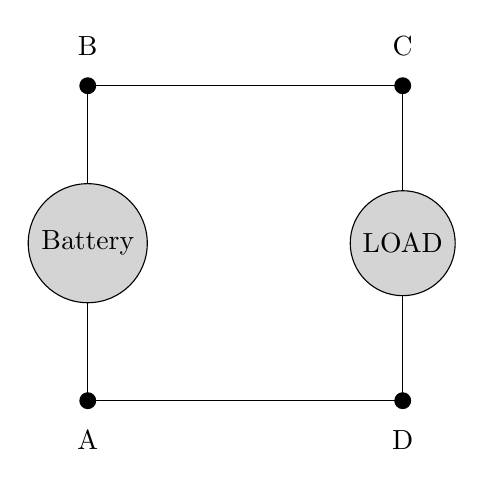
\begin{tikzpicture}
\draw (0,0)--(0,2) node[circle, draw=black,radius=0.25cm, fill={rgb:black,1;white,5}] {Battery}
--(0,4)--(4,4)--(4,2) node[circle, draw=black,radius=0.25cm, fill={rgb:black,1;white,5}] {LOAD}
--(4,0)--cycle;
\filldraw (4,0) circle[radius=1 mm]; \draw node at (4,-.5) {D};
\filldraw (4,4) circle[radius=1 mm]; \draw node at (4,4.5) {C};
\filldraw (0,4) circle[radius=1 mm]; \draw node at (0,4.5) {B};
\filldraw (0,0) circle[radius=1 mm]; \draw node at (0,-.5) {A};
\end{tikzpicture}
\label{F:2BL}
\end{center}
\end{figure}

For example, the network edge from B to C as drawn in Figure~\ref{F:2BL} represents a perfect wire because it was drawn as a line.
\par
\noindent
\begin{itemize}
\item \textbf{Observation:} If a perfect wire connects two nodes, these nodes will be at the same potential (voltage) and behave as one big node.\footnote{You can always decide that a some collection of nodes will be treated as one big node (sometimes called a supernode).} 
\item \textbf{Observation:} The length of a perfect wire does not matter. We'll usually draw whichever length makes the diagram most readable.
\item \textbf{Observation:} When wires cross, a dot indicates a connection.
\end{itemize}
%%%%%%%%%%%%%%%%%%%%%%%%%%%%%%%%%%%%%%%%%%%%%%%%%%%%%%%%%%%%%%%%%%%
\subsection{Switches}
A perfect switch provides a break in the wire when \emph{open} and acts as a perfect wire when \emph{closed}. Figure~\ref{F:2BLa} shows a battery connected to a load via a switch.

\begin{figure}[H]
\begin{center}
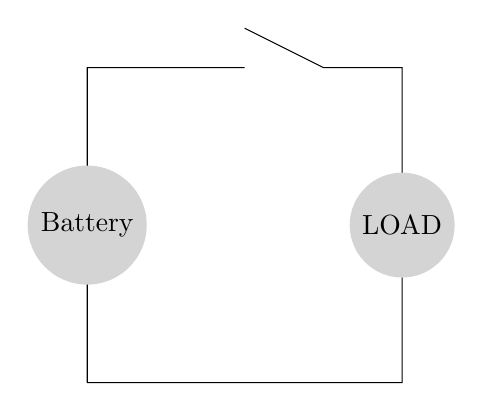
\begin{tikzpicture}
\draw (0,0) node(A){}
--(0,2) node[circle, radius=0.25cm, fill={rgb:black,1;white,5}] {Battery}
--(0,4)--(2,4) (2,4.5)--(3,4)--(4,4)
--(4,2) node[circle, radius=0.25cm, fill={rgb:black,1;white,5}] {LOAD}
--(4,0)
--(0,0);
\end{tikzpicture}
\caption{Battery connected to a load}
\label{F:2BLa}
\end{center}
\end{figure}

When the switch is open, the circuit has three nodes, labeled A, B and C as shown in Figure~\ref{F:2BLb}:

\begin{figure}[H]
\begin{center}
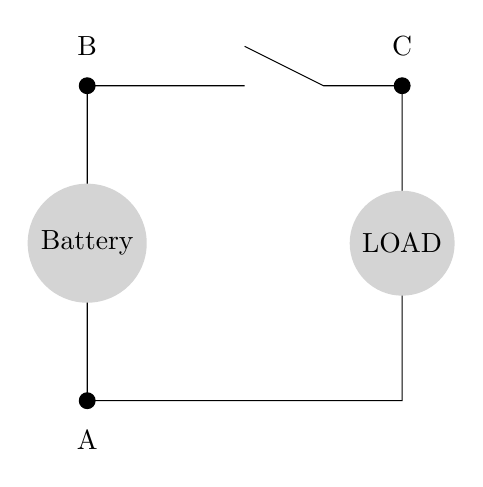
\begin{tikzpicture}
\draw (0,0) node(A){}
--(0,2) node[circle, radius=0.25cm, fill={rgb:black,1;white,5}] {Battery}
--(0,4)--(2,4) (2,4.5)--(3,4)--(4,4)
--(4,2) node[circle, radius=0.25cm, fill={rgb:black,1;white,5}] {LOAD}
--(4,0)--(0,0);
\filldraw (0,0) circle[radius=1 mm]; \draw node at (0,-.5) {A};
\filldraw (0,4) circle[radius=1 mm]; \draw node at (0,4.5) {B};
\filldraw (4,4) circle[radius=1 mm]; \draw node at (4,4.5) {C};
\end{tikzpicture}
\caption{Battery connected to a load with nodes indicated.}
\label{F:2BLb}
\end{center}
\end{figure}

When the switch is closed, the network has only two nodes. Nodes B and C become the same node, because they are connected with a perfect wire.\\
\linebreak
Many homes have three-way switches. The national electric code requires them for some situations like stairwells. With a three-way switch, one can turn off the stairwell light from the top or bottom of the staircase.
\par
Figure~\ref{F:23W} shows how such a switch might operate. The blue wire is the ground wire. We'll discuss that wire and its purpose later.
\par
\begin{figure}[H]
\begin{center}
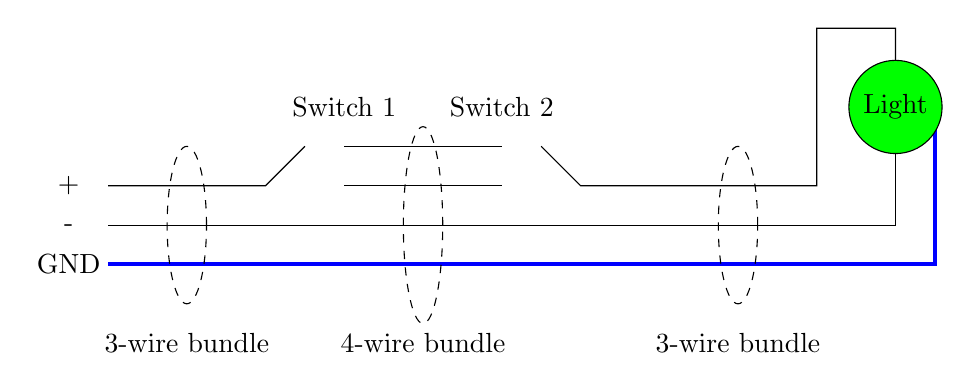
\begin{tikzpicture}
\draw [draw=blue, line width=0.5mm] (0,0) --(10.5,0)--(10.5,2) node(A){};
\draw (0,.5)--(10,0.5)--(10,2);
\draw (0,1)--(2,1)--(2.5,1.5);
\draw (3,1.5)--(5,1.5);
\draw (3,1)--(5,1);
\draw (5.5,1.5)--(6,1)--(9,1)--(9,3)--(10,3)--(10,2) node[circle,radius=.5cm,fill=green,draw=black](L) {Light};
\node at (3,2) {Switch 1};
\node at (5,2) {Switch 2};
\node at (1,-1) {3-wire bundle};
\node at (4,-1) {4-wire bundle};
\node at (8,-1) {3-wire bundle};
\draw [dashed] (1,.5) ellipse (.25 cm and 1 cm);
\draw [dashed] (4,.5) ellipse (.25 cm and 1.25 cm);
\draw [dashed] (8,.5) ellipse (.25 cm and 1 cm);
\node at (-.5,1) {+};
\node at (-.5,.5) {-};
\node at (-.5,0) {GND};
\end{tikzpicture}
\caption{Diagram showing a possible connection for a three-way switch. Note that a special wire with four leads is needed between the two switches.}
\label{F:23W}
\end{center}
\end{figure}

\begin{clevel}
Someone wants to wire a light where any of 3 switches can turn it on or off. Draw an appropriate sketch to show how that might be done. Include the ground wire in your sketch. Hint: You might need to invent another type of switch called a 4-way switch.
\end{clevel}

%%%%%%%%%%%%%%%%%%%%%%%%%%%%%%%%%%%%%%%%%%%%%%%%%%%%%%%%%%%%%%%%%%%%%%
\subsection{The Third Prong}
A plug designed for a wall outlet has three prongs. It is easy to imagine why we need two of them, but what is the purpose of the third prong? After all, some electrical products only have two prongs.\par

If one were to measure the voltages at each prong compared to GND, one of the prongs would read 120 V while the other two would both read zero\footnote{This is 120 VAC rms. We'll get to this later.}. Why do we need the third wire?\par

The reason involves safety. High voltages (like 120V) are dangerous. Consider the electric light shown in this diagram:

\par
\begin{figure}[H]
\begin{center}
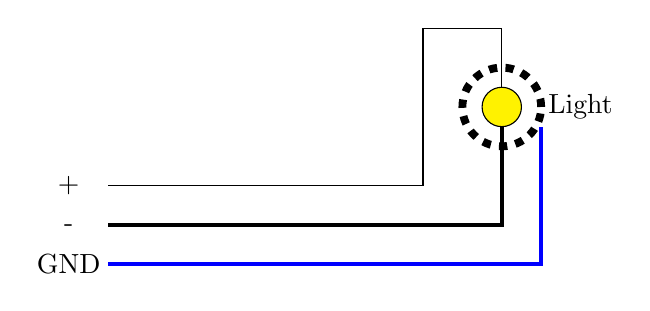
\begin{tikzpicture}
\draw [draw=blue, line width=0.5mm] (0,0) --(5.5,0)--(5.5,1.75) node(A){};
\draw [draw=black, line width=0.5mm] (0,.5)--(5,0.5)--(5,1.75);
\draw (0,1)--(4,1)--(4,3)--(5,3);
% (5,2); node[circle,radius=1cm,draw=black, line width=0.5 mm](L) {Light};
\draw (5,3)--(5,2.25);
\node[draw,circle,minimum size =0.5cm, fill=yellow] at (5,2){};
\node[draw,circle,minimum size =1cm, line width=1 mm, dashed] at (5,2){};
\node at (-.5,1) {+};
\node at (-.5,.5) {-};
\node at (-.5,0) {GND};
\node at (6,2) {Light};
\end{tikzpicture}
\caption{Light fixture showing ground wire protection. The dashed line represents the fixture's metal casing.}
\label{F:23P}
\end{center}
\end{figure}

Consider the situations shown in Table~\ref{T:2P3}:\par
\begin{table}[H]
\begin{center}
\begin{tabular}{c|c|c|c}
two prong or three prong?&status&person touching casing&shock hazard?\\ \hline
2	&	no problem	& yes	& no\\ \hline
2	&	case 1		& no	& no\\ \hline
2	&	case 1		& yes	& \textbf{yes}\\ \hline
2	&	case 2		& yes	& no\\ \hline
3	&	no problem	& yes	& no\\ \hline
3	&	case 1		& no	& no\\ \hline
3	&	case 1		& yes	& no*\\ \hline
3	&	case 2		& yes	& no\\ \hline
\end{tabular}\par
\caption{Situations with 2-prong or 3-prong wiring}
\label{T:2P3}
\end{center}
\end{table}

\begin{itemize}
\item Case 1. The + and nuetral (-) wires have rusted and broken off the light. The +wire touches the light casing.
\item Case 2. The + and neutral (-) wires have rusted and broken off the light. The neutral (-) touches the light casing.
\end{itemize}

Consider case 1 with the + wire contacting the casing. If the casing is grounded via the extra wire (connected to the third prong), then as soon as the + wire comes into contact with the casing, a large current will flow from the + wire through the casing, through the third wire and back to the breaker box. This current will likely exceed the 10 or 15A limit for the circuit breaker. This current will trip the breaker and shut off the circuit. By the time a person unwittingly touches the casing, the circuit should be disconnected and the person should be OK.\par

Of course, the light will no longer work and someone might notice. When the person tries to reset the breaker, the breaker should immediately re-trip, indicating a problem and maybe a hazard.\par

\begin{blevel}
Draw a sketch like Figure~\ref{F:23P}, but for the situation occuring in row 7 of the table.
\end{blevel}
%%%%%%%%%%%%%%%%%%%%%%%%%%%%%%%%%%%%%%%%%%%%%%%%%%%%%%%%%%%%%%%%%%%%%%%
\subsection{Light-bulbs}
A light-bulb or LED is a device that converts electrical energy into photons that are visible to the human eye. Older incandescent light bulbs operate by making a wire so hot that it glows white. This type of bulb wastes most of the energy as heat. Think of it like using a campfire to light up a living room.
Newer bulbs, like LEDs, more directly create photons and are much more efficient.

\begin{alevel}
What does LED stand for?
\end{alevel}

\begin{blevel}
What is a diode?
\end{blevel}

\begin{alevel}
At what temperature must something be in order to glow red? Look it up online.
\end{alevel}

\subsection{Voltage sources}
A voltage source produces a constant voltage difference between two points, almost regardless of the amount of current that would be needed.
\par
Solar panels represent decent voltage sources because they produces roughly steady voltages. More sunlight allows the panel to provide more current and therefore more power, but the voltage remains roughly the same.
\par
A wall socket also represents a fairly ideal voltage source, at least until the current exceeds the limit for the circuit breaker at which point the voltage goes to zero. Wall sockets in the US produce about 120 Volts AC, and provide roughly the same voltage difference whether you draw 1 Amp of current or 10 Amps of current. 

\par
\subsection{Current sources}
Current sources provide steady currents instead of steady voltages. The symbols for voltage sources and current sources are shown in Figure~\ref{F:2SCV}.
\par

\begin{figure}[H]
\begin{center}
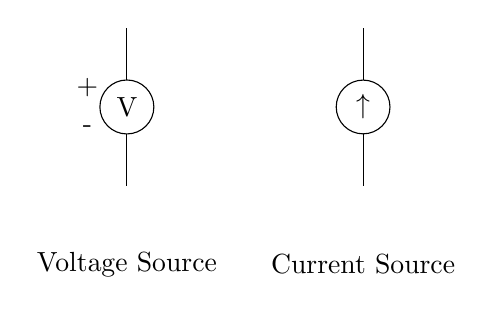
\begin{tikzpicture}
\node at (1,-1) {Voltage Source};
\node at (4,-1) {Current Source};
\draw (1,0)--(1,1) node[circle, draw=black, radius=1cm, fill=white]{V}--(1,2);
\node at (0.5,1.25) {+};
\node at (0.5,.75) {-};
\draw (4,0)--(4,1) node[circle, draw=black, radius=2cm, fill=white]{$\uparrow$}--(4,2);
\end{tikzpicture}
\caption{Symbols for voltage sources and current sources.}
\label{F:2SCV}
\end{center}
\end{figure}

Note the plus-minus indication on the voltage source. This indicates which side is more positive. The current source arrow already shows the direction of the current. If the current source were negative, then the current flows opposite the direction of the arrow.

\subsection{Resistors}
Unlike perfect wires, resistors are so named because they hinder or \emph{resist} the flow of current. It takes effort (energy) to push charge through a resistor. The more charge per second you need to get through the resistor, the more energy (effort) it will take.
\par
\begin{alevel}
What is another name for energy per charge?
\end{alevel}

For some objects, like a typical chunk of metal, the flow (current) varies roughly proportionally to the change in the voltage across it. This is captured by something called Ohm's Law.
\par
\begin{align*}
\Delta V \sim I	&&\text{Ohm's Law}
\end{align*}

The proportionality constant can be written as R.\par
\begin{align}
\Delta V = IR	&&\text{Ohm's Law}
\end{align}
 Note: the $\Delta$ on the $\Delta V$ is often omitted because it is usually obvious that you're referring to a change in voltage, and not some meaningless absolute voltage with respect to who-knows-what reference point. \par

\begin{alevel}
What is the standard S.I. unit of resistance?
\end{alevel}

\begin{clevel}
In terms of Coulombs, seconds, and Joules, what are the units of resistance?
\end{clevel}

\begin{clevel}
In terms of Coulombs, seconds, meters, and kg, what are the units of resistance? Hint: What is a Joule?
\end{clevel}

For better or worse, Ohm's law is NOT some fundamental relationship that is true all the time. Instead, it is only sort-of true some of the time. Manufactured resistors, like the ones in the lab, are designed mimic Ohm's Law pretty well. Other devices, like LEDs, do not much behave this way at all.\par

\begin{blevel}
Which of the following formulae are perfectly accurate (either because its a definition or because it is a model that has not (yet) been contradicted by experiment) verses a approximate model (hack) that we know is not exactly right?\\
\begin{center}
\begin{tabular}{|c|c|}\hline
equation & (always correct) or (hack)? \\ \hline
$F_f=\mu F_N$ & \\ \hline
$V=IR$ & \\ \hline
$\rho=\frac{mass}{Vol}$ & \\ \hline
$PV=nRT$ & \\ \hline
\end{tabular}
\end{center}
\end{blevel}

Resistors on a diagram are drawn with a zig-zag line. Figure~\ref{F:21} shows a current source connected to a $5 \Omega$ resistor.

\begin{figure}[H]
\begin{center}
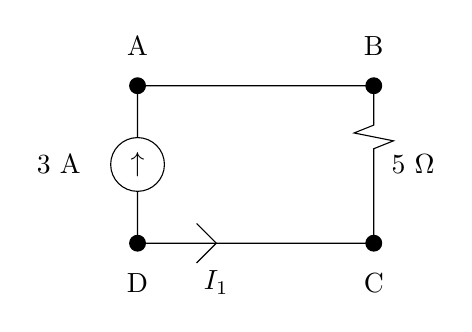
\begin{tikzpicture}
\draw (1,0)--(1,1) node[circle, draw=black, radius=2cm, fill=white]{$\uparrow$}--(1,2)--(4,2)--(4,1.5)--(3.75,1.4)--(4.25,1.3)--(4,1.2)--(4,0)--(1,0);
\node at (0,1) {3 A};
\node at (4.5,1) {5 $\Omega$};
\filldraw (1,2) circle[radius=1 mm];
\node at (1,2.5) {A};
\filldraw (4,2) circle[radius=1 mm];
\node at (4,2.5) {B};
\filldraw (4,0) circle[radius=1 mm];
\node at (4,-.5) {C};
\filldraw (1,0) circle[radius=1 mm];
\node at (1,-.5) {D};
\draw (1.75,.25)--(2,0)--(1.75,-.25);
\node at (2,-.5) {$I_1$};
\end{tikzpicture}
\caption{A current source connected to a resistor. Note how current $I_1$ is labeled with an arrow.}
\label{F:21}
\end{center}
\end{figure}

\begin{blevel}
Fill in Table~\ref{T:21}.
\end{blevel}

\begin{table}[H]
\begin{center}
\begin{tabular}{|c|c|c|}\hline
item&answer&hints\\ \hline
$I_1$	&	&	\\ \hline
$V_{AB}$	&	&	\\ \hline
$V_{BC}$	&	& use Ohm's law	\\ \hline
$V_{AD}$	&	&	\\ \hline
$I_{from B to C}$	&	&	\\ \hline
Power absorbed by R	&	&	\\ \hline
Power produced by current source	&	&	\\ \hline
\end{tabular}
\label{T:21}
\caption{Summary of select parameters for simple circuit.}
\end{center}
\end{table}

One can connect resistance (an extrinsic property) to resistivity (an intrinsic property). \footnote{An \textbf{extrinsic} property depends on something's amount or shape. An \textbf{intrinsic} property does not depend on how much of it you have. Density is an intrinsic property whereas mass is not.}\par

\begin{align}
R = \rho \frac{L}{A} \label{E:2rho}
\end{align}
Where $\rho$ is the resistivity of the material, L is its length and A is its cross-sectional area.

\begin{blevel}
Determine the resistance of a 20 m long section of 12 gauge copper wire. Hint: look up the radius of 12 gauge wire. 12-gauge wire is typical for household wiring.
\end{blevel}

\begin{blevel}
An aluminum wire inside a computer chip carries a signal from one side of the chip to the other. The dimensions of the wire are 5 mm by 1 micron by 0.1 micron. What is the resistance of the wire? If 100mA of current pass through the wire, what is the voltage dropped across it? How much power is dissipated by the wire? 
\end{blevel}

\begin{dlevel}
Continuing the previous problem. If the heat had nowhere to go but to heat up the Al wire, how much would the temperature of the wire increase after 1 minute? How much time until the wire melted?
\end{dlevel}

We can substitute Equation~\eqref{E:2rho} expression for resistance into Ohm's law and come up with an equation for electricity flow that is very similar to the flow of heat.

\begin{align*}
I = \frac{\Delta V}{R}	\\
\frac{dq}{dt} = \frac{\Delta V}{\rho}\frac{A}{L}=(\frac{1}{\rho})\frac{A\Delta V}{L}&&	\text{``electricity flow" equation}\\
\frac{dQ}{dt}=	\frac{kA\Delta T}{L}&&				\text{heat flow equation}
\end{align*}
What drives heat to flow from one side of a material to the other? Answer: a temperature difference. What drives electrical charge to flow from one side of a material to the other? Answer: a voltage difference.

\begin{blevel}
A 0.5 meter long section of 12-gauge Cu wire connects between the inside of a house ($65^0 F$) and the outside of a house ($35^0 F$). How many Joules of heat flow out of the house through the wire in one minute?
\end{blevel}

\begin{blevel}
A 0.5 meter long section of 12-gauge Cu wire connects between one side of a 9V battery and the other. How many Coulombs of charge flow along the wire in one minute?
\end{blevel}


\chapter{Basic Analysis Principles}
In this chapter, we'll use three fundamental principles to analyze electrical networks (circuits). Some of these tools apply to other types of networks as well.

\begin{enumerate}
\item Net current into a node equals zero. ($\sum{I_{IN}}=0$) \underline{Be careful, not always true.}
\item Voltage around loop equals zero. ($\sum{V_{LOOP}}=0$) \underline{Be careful, not always true.}
\item Power In = Power Out (Conservation of Energy). \underline{Be careful!}
\end{enumerate}

\par
These principles lead to constraints (limitations) which determine the voltage or current values the electrical network can have. Constraints lead to equations. Constraints help us narrow in on how the circuit must behave.

\BI{Equations represent statements about a situation that must be true. If you have too many equations, it becomes impossible to make them all true at the same time. If you have few equations, there might be many ways to make them true.}

%%%%%%%%%%%%%%%%%%%%%%%%%%%%%%%%%%%%%%%%%%%%%
\subsection{Basic tool I}

\textbf{The net current into a node equals zero}. Consider items leaving as equivalent to a negative number of items entering. According to this principle, the currents into a node must equal the currents leaving that node. We might call this the in=out rule. This assumes two things:

\begin{itemize}
\item That the charge at a node can not increase or decrease significantly. It certainly can't increase forever\footnote{If infinite charge were to accumulate on a node, it would take infinite energy to add more charge to it - good luck with that.}. For our traffic network, this principle would apply if none of the towns had any parking. In that case, the cars entering the town must always match the number of cars leaving the town.
\item That charge can not be created or destroyed (that electric charge is conserved). Were it not for this, charge could go into a node and be destroyed, like garbage going into an incinerator. This principle is pretty safe.
\end{itemize}
\par

\BI{Look to identify conserved quantities, like electric charge. Conserved quantities lead to constraints and equations that describe the system.}\par

\par
This in=out constraint is sometimes called Kirchoff's Current Law, or KCL.
\par
\begin{align*}
\Sigma I_{entering}=0	&&\text{KCL}
\end{align*}

KCL holds for each node, so if a circuit has 5 nodes, you get 5 equations.

\begin{blevel}
A box begins with 20C of charge. 5 Amps enters the box for 2 minutes, then 10 minutes later 7 Amps leaves the box for 1 minute. Determine the final amount of charge in the box.
\end{blevel}

\begin{dlevel}
Conservation of mass can be useful. Does it always apply? If not, when would it not apply? Would it apply when tracking all the food entering and leaving a cafeteria? If not, what would you need to do to make it apply?
\end{dlevel}

\begin{blevel}
Determine which these situations would be consistent, approximately consistent, or not at all consistent with the in=out principle:
\begin{itemize}
\item Total liquid gasoline going into and out of a car.
\item Electric charge going into and out of a node.
\item Liquid gasoline going into and out of a gas station, including delivery trucks.
\item The mass of water going into and out of a plumbing junction.
\end{itemize}
\end{blevel}

%%%%%%%%%%%%%%%%%%%%%%%%%%%%%%%%%%%%%%%
\subsection{Basic Tool II. }
\textbf{The sum of the voltage differences around any loop in the circuit equals zero.} In our hiking trail example earlier, if you start hiking at point A and end at point A, the total change in elevation would be zero. Therefore the total change in gravitational potential (gravitational potential energy per mass) would be zero. We can generalize this statement for trail networks as follows:
\par

\begin{align}
\Sigma V_g(loop)=0	&&\text{Trail System Law}
\end{align}

A similar rule holds for electrical networks, and for the same reasons. We call this Kirchoff's Voltage Law, or KVL. 

\begin{align}
\Sigma V(loop)=0	&&\text{KVL}
\end{align}

Unfortunately, like KCL, KVL is also not \emph{always} true\footnote{Whether or not it is unfortunate depends on your point of view. The exceptions to this rule are pretty important to how the whole world works.}. The presence of changing magnetic fields can cause the sum of the voltages around a loop to be other than zero.

\begin{alevel}
Suppose an electrical network has 3 nodes, A, B and C. Furthermore $V_{AB}=2$ V and $V_{BC}=3$ V. Determine $V_{AC}$.
\end{alevel}

\subsection{Basic Tool III.} 
\textbf{Power put into a circuit (from sources) equals power out (dissipated as heat or as work done on something outside the circuit}. This assumes that the amount of potential energy stored in the network is fixed, which does not need to be the case.\par

\begin{alevel}
A 5 V battery sends 3 Amps of current into a circuit consisting of just one resistor. How much energy does the resistor dissipate as heat each second?
\end{alevel}

\section{Sample Circuit}
We will now analyze the circuit in Figure~\ref{F:3CKT} using the above tools. We'll introduce a make-believe component called a \emph{Gator}, indicated by the $\Rightarrow$ symbol. A Gator behaves such that there is always a 2V drop across it (the arrow points to the more positive side).

\par
The voltage V is +5V.
\par

\begin{figure}[H]
\begin{center}
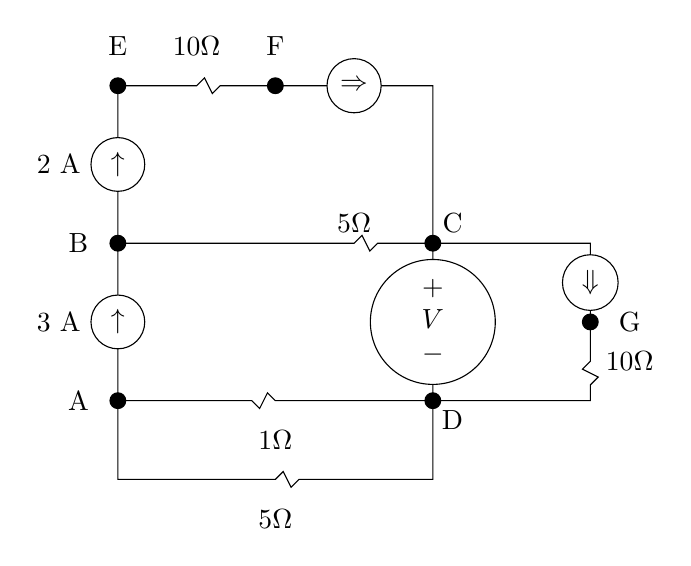
\begin{tikzpicture}
\draw (1,0)--(1,1) node[circle, draw=black, radius=2cm, fill=white]{$\uparrow$}
--(1,2)--(4,2)--(4.1,2.1)--(4.2,1.9)--(4.3,2)--(5,2);
\node at (4,2.25) {$5 \Omega$};
\node at (0.25,1) {3 A};
\node at (0.25,3) {2 A};
\node at (7.5,.5) {$10 \Omega$};
\node at (2,4.5) {$10 \Omega$};
\node at (3,-.5) {$1 \Omega$};
\node at (3,-1.5) {$5 \Omega$};
\filldraw (1,0) circle[radius=1 mm];
\node at (.5,0) {A};
\filldraw (1,2) circle[radius=1 mm];
\node at (.5,2) {B};
\filldraw (5,2) circle[radius=1 mm];
\node at (5.25,2.25) {C};
\filldraw (5,0) circle[radius=1 mm];
\node at (5.25,-.25) {D};
\filldraw (1,4) circle[radius=1 mm];
\node at (1,4.5) {E};
\filldraw (3,4) circle[radius=1 mm];
\node at (3,4.5) {F};
\filldraw (7,1) circle[radius=1 mm];
\node at (7.5,1) {G};
\draw (1,2)--(1,3) node[circle, draw=black, radius=2cm, fill=white]{$\uparrow$}
--(1,4)--(2,4)--(2.1,4.1)--(2.2,3.9)--(2.3,4)
--(4,4) node[circle, draw=black,radius=2cm, fill=white]{$\Rightarrow$}
--(5,4)--(5,2)
--(5,1) node[circle, draw=black, radius=2cm, fill=white]{$\begin{matrix}+\\V\\-\end{matrix}$}
--(5,0)--(3,0)--(2.9,.1)--(2.8,-.1)--(2.7,0)--(1,0);
\draw (5,2)--(7,2)
--(7,1.5) node[circle, draw=black,radius=2cm, fill=white]{$\Downarrow$}
--(7,.5)--(6.9,.4)--(7.1,.3)--(7,.2)--(7,0)--(5,0);
\draw (1,0)--(1,-1)--(3,-1)--(3.1,-.9)--(3.2,-1.1)--(3.3,-1)--(5,-1)--(5,0);
\end{tikzpicture}
\caption{A circuit for analysis.}
\label{F:3CKT}
\end{center}
\end{figure}

There are many places to start, so the plan below outlines just one way to do it.

\begin{enumerate}
\item Find the current from B to C through the 5 $\Omega$ resistor. Use KCL.
\item Use Ohm's Law to determine the voltage drop from B to C. For a resistor, a positive current will always flow from a positive voltage to negative voltage.\footnote{For sources, the current can flow either direction depending on whether the source is absorbing power or producing power.}
\item Identify the current through point E. Use Ohm's Law to determine the voltage $V_{EF}$.
\item Use KVL to determine the voltage drop across the 2A current source.
\item Use KVL to determine the voltage drop across the 10 Ohm resistor, $V_{GD}$.
\item Use Ohm's Law to determine the current from node G to node D (through the 10 Ohm resistor).
\end{enumerate}

Answers are now in blue.

\begin{figure}[H]
\begin{center}
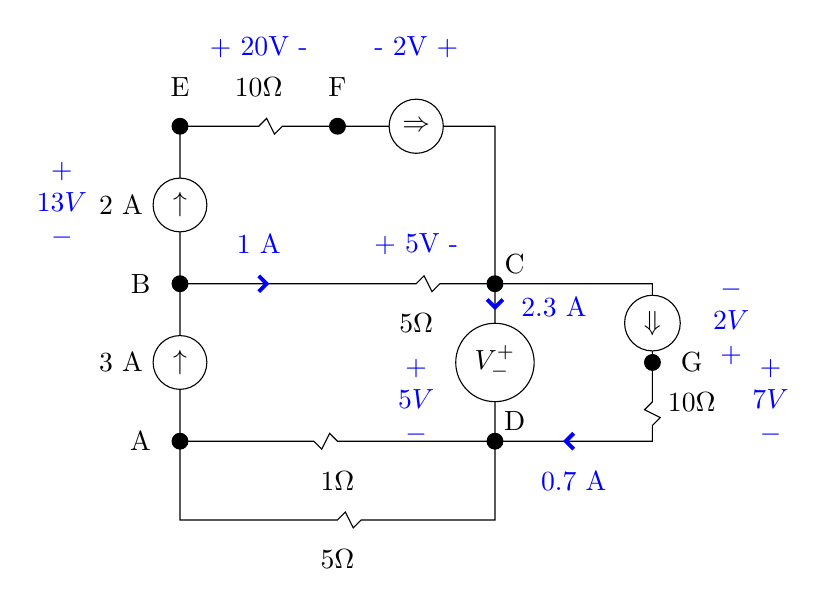
\begin{tikzpicture}
\draw (1,0)--(1,1) node[circle, draw=black, radius=2cm, fill=white]{$\uparrow$}
--(1,2)--(4,2)--(4.1,2.1)--(4.2,1.9)--(4.3,2)--(5,2);
\node at (4,1.5) {$5 \Omega$};
\node at (0.25,1) {3 A};
\node at (0.25,3) {2 A};
\node at (7.5,.5) {$10 \Omega$};
\node at (2,4.5) {$10 \Omega$};
\node at (3,-.5) {$1 \Omega$};
\node at (3,-1.5) {$5 \Omega$};
\filldraw (1,0) circle[radius=1 mm];
\node at (.5,0) {A};
\filldraw (1,2) circle[radius=1 mm];
\node at (.5,2) {B};
\filldraw (5,2) circle[radius=1 mm];
\node at (5.25,2.25) {C};
\filldraw (5,0) circle[radius=1 mm];
\node at (5.25,.25) {D};
\filldraw (1,4) circle[radius=1 mm];
\node at (1,4.5) {E};
\filldraw (3,4) circle[radius=1 mm];
\node at (3,4.5) {F};
\filldraw (7,1) circle[radius=1 mm];
\node at (7.5,1) {G};
\draw (1,2)--(1,3) node[circle, draw=black, radius=2cm, fill=white]{$\uparrow$}
--(1,4)--(2,4)--(2.1,4.1)--(2.2,3.9)--(2.3,4)
--(4,4) node[circle, draw=black,radius=2cm, fill=white]{$\Rightarrow$}
--(5,4)--(5,2)
--(5,1) node[circle, draw=black, radius=2cm, fill=white]{$V_{-}^{+}$}
--(5,0)--(3,0)--(2.9,.1)--(2.8,-.1)--(2.7,0)--(1,0);
\draw (5,2)--(7,2)
--(7,1.5) node[circle, draw=black,radius=2cm, fill=white]{$\Downarrow$}
--(7,.5)--(6.9,.4)--(7.1,.3)--(7,.2)--(7,0)--(5,0);
\draw (1,0)--(1,-1)--(3,-1)--(3.1,-.9)--(3.2,-1.1)--(3.3,-1)--(5,-1)--(5,0);
\draw [draw=blue, line width=0.5mm] (2,2.1)--(2.1,2)--(2,1.9);
\node [text=blue] at (2,2.5) {1 A};
\draw [draw=blue, line width=0.5mm] (6,.1)--(5.9,0)--(6,-.1);
\node [text=blue] at (6,-.5) {0.7 A};
\draw [draw=blue, line width=0.5mm] (4.9,1.8)--(5,1.7)--(5.1,1.8);
\node [text=blue] at (5.75,1.7) {2.3 A};
\node [text=blue] at (2,5) {+ 20V -};
\node [text=blue] at (4,5) {- 2V +};
\node [text=blue] at (4,2.5) {+ 5V -};
\node [text=blue] at (-.5,3) {$\begin{matrix}+\\13V\\-\\\end{matrix}$};
\node [text=blue] at (8,1.5) {$\begin{matrix}-\\2V\\+\\\end{matrix}$};
\node [text=blue] at (4,.5) {$\begin{matrix}+\\5V\\-\\\end{matrix}$};
\node [text=blue] at (8.5,.5) {$\begin{matrix}+\\7V\\-\\\end{matrix}$};
\end{tikzpicture}
\caption{The circuit with most of the solutions.}
\label{F:3CKTb}
\end{center}
\end{figure}

We've got \emph{almost} everything, but we're still missing the voltages across and currents through the 1 $\Omega$ and 5 $\Omega$ resistors. It seems like we can't get those values in one easy step, like we did for the others. But don't worry, we just need to write down what we know and then do a little algebra.
\par

Here's what we know.
\begin{itemize}
\item From KCL, the currents $I_1$ (the current through the 1$\Omega$ resistor) and $I_5$ (the current through the 5$\Omega$ resistor) must add up to 3A. $I_1+I_5=3$
\item From Ohm's Law, we know that $V_{AD}=I_1*1$ and $V_{AD}=I_5*5$. 
\item We have three equations and three uknowns. We can solve. 
\end{itemize} 

\begin{blevel}
Solve for $I_1,I_5,V_{AD}$. 
\end{blevel}

\begin{clevel}
Use this answer and KVL to determine the voltage across the 3A current source.
\end{clevel}

Finally, we check our answer using conservation of energy/power (basic tool III). If the current and voltage are the same direction, then power is consumed. If they are opposite directions (we'll indicate this with a + sign), then power is being added to the circuit (we'll indicate this with a - sign).

\begin{clevel}
Fill in Table~\ref{F:3CKT3}.
\end{clevel}

\begin{table}[H]
\begin{center}
\begin{tabular}{|c|c|c|c|} \hline
component &	current through it	& voltage across it	& power consumed \\ \hline
2A source	&+2A			&-13V (V, I in opp. dirs.)	&-26Watts\\ \hline
3A source	&			&	&	\\ \hline
10 Ohm (E-F)	&+2A			&+20V	&+40W	\\ \hline
5 Ohm (B-C)	&			&	&	\\ \hline
10 Ohm (G-D)	&			&	&	\\ \hline
1 Ohm (A-D)	&			&	&	\\ \hline
5 Ohm (A-D)	&			&	&	\\ \hline
5V source	&			&	&	\\ \hline
Gator Top	&			&	&	\\ \hline
Gator Side	&			&	&	\\ \hline
\end{tabular}
\caption{Table to check conservation of energy.}
\label{F:3CKT3}
\end{center}
\end{table}

\begin{clevel}
What does your total power sum to? It should be zero if the power produced matches the power consumed.
\end{clevel}

\begin{clevel}
Recreate a duplicate of the Table~\ref{F:3CKT3} but for the case where every resistor has a value of 10 Ohms.
\end{clevel}

%%%%%%%%%%%%%%%%%%%%%%%%%%%%%%%%%%%%%%%%%%%%%%%%%%%%%%%%%%%%
\section{Equivalent Combinations}
In this section, we'll look for ways to simplify electrical networks. We'll simplify by finding a simpler circuit that is equivalent. This is exactly what you do in algebra when you simplify $3x+4x$ by writing $7x$. The $7x$ is often simpler to work with and is mathematically equivalent.\par

\vspace{3 mm}
\BI{Look for ways to simplify a model. Combine like terms. Combine multiple forces into one. Combine resistors.}\vspace{3 mm}

In this section, we'll combine resistors in series and in parallel. 


\BI{Learn something once, apply it many times. See series and parallel combinations in many areas. Resistors can be combined in series or in parallel, but so can springs or tasks or hoses or many other things.}

Let's study the series combination of resistors first. 

\par

%%%%%%%%%%%%%%%%%%%%%%%%%%%%%%%%%%%%%%%%%%%%%%%%%
\subsection{Series combination}
Two two-terminal components are in series if:
\begin{itemize}
\item One side of one component shares a node with one side of the other component.
\item No other current paths (like a wire) connect to the shared node \footnote{There just can't be any other current leaving the shared node. A wire carrying no current could connect to the shared node.}.
\end{itemize}

We'd like to replace the series combination of two resistors, $R_1$ and $R_2$ with one resistor ($R_T$) such that the two circuits equivalent. To be equivalent, the two circuits shown in Figure~\ref{F:2SER} then must have the same voltages from A to C and the same current from A to C.

\begin{figure}[H]
\begin{center}
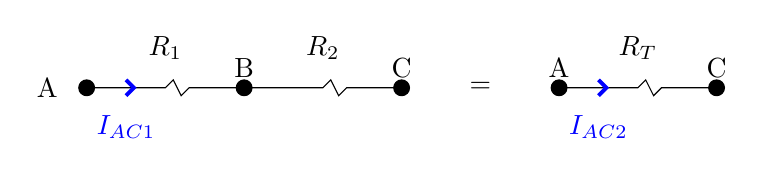
\begin{tikzpicture}
\node at (2,.5) {$R_1$};
\node at (4,.5) {$R_2$};
\filldraw (1,0) circle[radius=1 mm];
\node at (.5,0) {A};
\filldraw (3,0) circle[radius=1 mm];
\node at (3,.25) {B};
\filldraw (5,0) circle[radius=1 mm];
\node at (5,.25) {C};
\draw (1,0)--(2,0)--(2.1,.1)--(2.2,-.1)--(2.3,0)--(3,0);
\draw (3,0)--(4,0)--(4.1,.1)--(4.2,-.1)--(4.3,0)--(5,0);
\draw [draw=blue, line width=0.5mm] (1.5,.1)--(1.6,0)--(1.5,-.1);
\node [text=blue] at (1.5,-.5) {$I_{AC1}$};
\node at (6,0) {=};
%
\node at (8,.5) {$R_T$};
\filldraw (7,0) circle[radius=1 mm];
\node at (7,0.25) {A};
\filldraw (9,0) circle[radius=1 mm];
\node at (9,.25) {C};
\draw (7,0)--(8,0)--(8.1,.1)--(8.2,-.1)--(8.3,0)--(9,0);
\draw [draw=blue, line width=0.5mm] (7.5,.1)--(7.6,0)--(7.5,-.1);
\node [text=blue] at (7.5,-.5) {$I_{AC2}$};
\end{tikzpicture}
\caption{A series combination of resistors and its equivalent resistance.}
\label{F:2SER}
\end{center}
\end{figure}

To determine the combined resistance, $R_T$, we'll do the following:
\begin{enumerate}
\item Observe that to be equivalent: $I_{AC1}=I_{AC2}=I_{AC}$.
\item Observate that to be equivalent $V_{AC}$ must be the same for both.
\item By Ohm's Law, $V_{AC2}=I_{AC}*R_T$
\item By Ohm's Law and KVL\footnote{By KVL, $V_{AC}$ must match $V_{AB}+V_{BC}$}, $V_{AC}=I_{AC}*R_1+I_{AC}*R_2$.
\item Therefore, $I_{AC}*R_T=I_{AC}*R_1+I_{AC}*R_2$.
\item Factor out $I_{AC}$ and cancel. 
\item Conclusion: $R_T=R_1+R_2$.
\end{enumerate}

\begin{alevel}
A 3 $\Omega$ resistor is connected in series with a 5 $\Omega$ resistor. If this combination were replaced with one resistor, what resistance would it have?
\end{alevel}

\begin{clevel}
Prove that for three resistors in series: $R_T=R_1+R_2+R_3$
\end{clevel}

\begin{clevel}
Consider a length of wire (length L) with a uniform cross sectional area A. Imagine this wire being divided into two lengths, $L_1$ and $L_2$. Show that our formula for series combination ($R_T=R_1+R_2$) is equivalent to claiming that $L=L_1+L_2$. 
\end{clevel}

%%%%%%%%%%%%%%%%%%%%%%%%%%%%%%%%%%%%%%%%%%%%%%%%%%%%%%%%
\subsection{Parallel Combination}
Two two-terminal components are in parallel if:
\begin{itemize}
\item One side of one component shares a node with one side of the other component (they are touching).
\item The other two terminals of the two components also share a node (are touching).
\end{itemize}

\begin{alevel}A 3 $\Omega$ resistor is connected in parallel with a 5 $\Omega$ resistor. If this combination were replaced with one resistor, what resistance would it have?
\end{alevel}

\begin{clevel}
Use a similar strategy to prove the for two resistors in parallel, $\frac{1}{R_T}=\frac{1}{R_1}+\frac{1}{R_2}$.
\end{clevel}

\begin{clevel}
Consider a length of wire (length L) with a uniform cross sectional area A. Imagine this wire being divided lengthwise into two strips, both the same length as the original but so that each strip has only part of the original cross sectional area, $A_1$ and $A_2$. Show that our formula for parallel combination ($\frac{1}{R_T}=\frac{1}{R_1}+\frac{1}{R_2}$) is equivalent to claiming that $A=A_1+A_2$. 
\end{clevel}

\begin{clevel}
Starting with: $\frac{1}{R_T}=\frac{1}{R_1}+\frac{1}{R_2}$, use algebra to show that $R_T=\frac{R_1 R_2}{R_1+R_2}$.
\end{clevel}

\begin{blevel}
Make a units based arguement that for three resistors in parallel, the following equation can't possibly be correct (no matter how much you want it to be.) $R_T=\frac{R_1 R_2 R_3}{R_1+R_2+R_3}$.
\end{blevel}

\begin{blevel}
Suppose you start with one resistor and then add another resistor in parallel to it. Does this make the combined resistance, go up, go down, or sometimes go up or down depending on the sizes of the two resistors?
\end{blevel}

\begin{dlevel}
Symmetric polynomials are polynomials where the variables can be swapped without changing the result. For example, $xy+xz+yz$ is a symmetry polynomial, but $xy+x$ is not. Consider four resistors in parallel. Define the symmetry polynomials:
\begin{align*}
S_1&=R_1+R_2+R_3+R_4 \\
S_2&=R_1R_2+R_1R_3+R_1R_4+R_2R_3+R_2R_4+R_3R_4\\
S_3&=R_1R_2R_3+R_1R_2R_4+R_1R_3R_4+R_2R_3R_4\\
S_4&=R_1R_2R_3R_4
\end{align*}
Show that the equivalent parallel combination is: $R_T = \frac{S_4}{S_3}$. In terms of the symmetry polynomials, what will be the parallel combination of N resistors in parallel?
\end{dlevel}

Consider the following diagram:

\begin{figure}[H]
\begin{center}
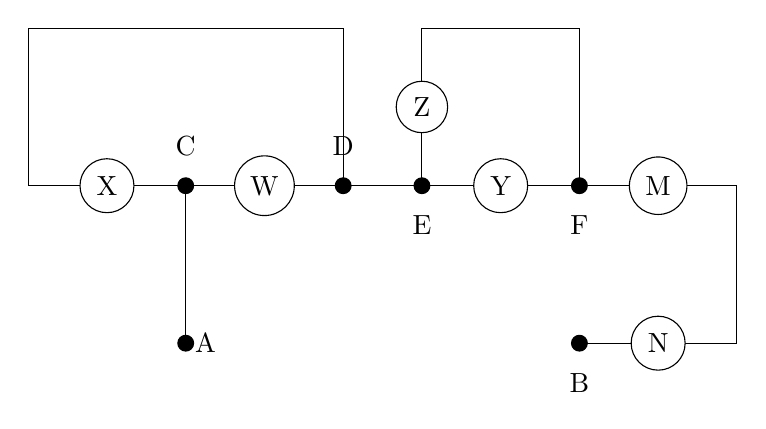
\begin{tikzpicture}
\draw (0,-2)--(0,0)--(-1,0) node[circle, draw=black,radius=2cm, fill=white]{X}
--(-2,0)--(-2,2)--(2,2)--(2,0)--(3,0)
--(4,0)node[circle, draw=black,radius=2cm, fill=white]{Y}
--(5,0)--(6,0)node[circle, draw=black,radius=2cm, fill=white]{M}
--(7,0)--(7,-2)--(6,-2)node[circle, draw=black,radius=2cm, fill=white]{N} 
--(5,-2);
\draw (0,0)--(1,0)node[circle, draw=black,radius=2cm, fill=white]{W}
--(2,0); 
\draw (3,0)--(3,1)node[circle, draw=black,radius=2cm, fill=white]{Z}
--(3,2)--(5,2)--(5,0);
\filldraw (0,-2) circle[radius=1 mm];
\node at (0.25,-2) {A};
\filldraw (5,-2) circle[radius=1 mm];
\node at (5,-2.5) {B};
\filldraw (0,0) circle[radius=1 mm];
\node at (0,.5) {C};
\filldraw (2,0) circle[radius=1 mm];
\node at (2,.5) {D};
\filldraw (3,0) circle[radius=1 mm];
\node at (3,-.5) {E};
\filldraw (5,0) circle[radius=1 mm];
\node at (5,-.5) {F};
\end{tikzpicture}
\caption{Series and Parallel Combination of Components.}
\label{F:SP3}
\end{center}
\end{figure}

\begin{clevel}
Fill in the Table~\ref{T:3SP} by identifying which components are in series, parallel or neither.
\end{clevel}

\begin{table}[H]
\begin{center}
\begin{tabular}{|c|c|} \hline
components & series, parallel or neither \\ \hline
X and W &	\\ \hline
Z and W &	\\ \hline
Y and M &	\\ \hline
N and M &	\\ \hline
Z and Y &	\\ \hline
X and M &	\\ \hline
\end{tabular}
\caption{Series or parallel?}
\label{T:3SP}
\end{center}
\end{table}

\begin{clevel}
Suppose components X,Y,W,Z,M and N were are resistors of value 10 Ohms. Determine the value of their combined resistance as measured from node A to B.
\end{clevel}

\begin{blevel}
The network shown in Figure~\ref{F:SP3} could be described from A to B as ($X \parallel W+Z \parallel Y+M+N$), where the parallel operation comes before the series operation. Draw a sketch of a circuit that matches:  $(X \parallel (W+Z)+A)\parallel Y+M$
\end{blevel}

\begin{blevel}
Draw a way to connect three 5 $\Omega$ resistors to create exactly 7.5 $\Omega$ of total resistance.
\end{blevel}

\begin{alevel}
Suppose current had to flow through a resistor from A to B. If additional resistors were added in series, would this make it easier or harder for current to flow?
\end{alevel}

\begin{clevel}
Consider the infinite resistor network shown in Figure~\ref{F:3TRANS}. All resistors are of size R. Determine the resistance from A to B, called $R_{AB}$. Hint: Because the network is infinite, the resistance to the right of C and D, $R_{CD}$, must equal $R_{AB}$. Write down $R_{AB}$ in terms of itself and solve. If you end with a quadratic equation, you're on the right track.
\end{clevel}

\begin{figure}[H]
\begin{center}
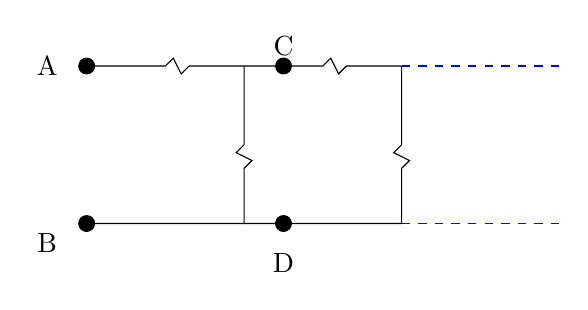
\begin{tikzpicture}
\filldraw (0,0) circle[radius=1 mm]; \draw node at (-.5,-.25) {B};
\filldraw (0,2) circle[radius=1 mm]; \draw node at (-.5,2) {A};
\filldraw (2.5,2) circle[radius=1 mm]; \draw node at (2.5,2.25) {C};
\filldraw (2.5,0) circle[radius=1 mm]; \draw node at (2.5,-.5) {D};
\draw (0,2)--(1,2)--(1.1,2.1)--(1.2,1.9)--(1.3,2)--(2,2);
\draw (2,2)--(2,1)--(1.9,.9)--(2.1,.8)--(2,.7)--(2,0)--(0,0);
\draw (2,2)--(3,2)--(3.1,2.1)--(3.2,1.9)--(3.3,2)--(4,2);
\draw (4,2)--(4,1)--(3.9,.9)--(4.1,.8)--(4,.7)--(4,0)--(2,0);
\draw [dashed, draw=blue] (4,2)--(6,2) (4,0)--(6,0);
\end{tikzpicture}
\caption{Infinite resistive network. Useful for modeling transmission lines.}
\label{F:3TRANS}
\end{center}
\end{figure}



\subsection{Conductance}
We saw earlier in equation ~\eqref{eq:2rho} that resistance depends on an intrinsic material property called resistivity, $\rho$, as well as its length and cross-sectional area. Longer wires have more resistance. Thicker wires have less resistance.\par

Could we just as easily define something called \textbf{conductance} which is just the reverse? Longer wires have less conductance and thicker wires have more. The answer is yes, just define conductance, G, as the inverse of resistance\footnote{We also define a quantity, conductivity which is the inverse of resistivity, but it doesn't capture any new information.}

\begin{align}
G=\frac{1}{R}=\frac{1}{\rho\frac{L}{A}}=\frac{A}{\rho L}&& \text{conductance}
\end{align}

Because $G=\frac{1}{R}$ and therefore $R=\frac{1}{G}$, then our series and parallel combination relationships look like:

\begin{align}
\frac{1}{G_T}=\frac{1}{G_1}+\frac{1}{G_2}&\leftarrow \text{series}\\
G_T=G_1+G_2&\leftarrow \text{parallel}
\end{align}

Notice that the parallel relationship is now the simpler one. We'll mostly use resistance in this book, and therefore you might get the impression that somehow parallel combinations are naturally more complicated, when, in fact, it is merely that we arbitrarily chose to use resistance instead of conductance.\par

The whole book could be done with conductance instead of resistance, and then you might grow to dislike series combinations instead of parallel ones. Love them both.

\begin{blevel}
Two resistors are connected in parallel. The first has a resistance of 5 $\Omega$ and the second has a conductance of 2 $\frac{1}{\Omega}$. Determine the combined conductance of this parallel combination.
\end{blevel}

%%%%%%%%%%%%%%%%%%%%%%%%%%%%%%%%%%%%%%%%%%%%%%%%%%%%%%%%%
\subsection{Application: Trust Networks}
We all get information from a variety of sources, family, friends, news sources, books, direct evidence, etc. Not all of pathways for the flow of information are equally trusted - maybe you trust Aunt X more than Uncle Z? The sum of all pathways that information flows from source(s) to a people could be modeled as a trust network.\par 

Let's apply what we've learned about combining resistors to trust networks. Trust networks involve series and parallel combinations of trust. For example, if A tells B something \textbf{and then} B tells C, this means that C must, at least partially, trust both A and B in order to trust the information. This situation represents a series chain of trust.\par

On the other hand, suppose A tells C and also B tells C. And suppose that A and B are independent sources \footnote{The idea of independence is important in algebra. In algebra it means that equations are not copies or combinations of each other. In this context, it means basically the same thing, that A and B each have their own reasons for believing something. It's not just that A told B and then they both told you.} then this would represent a parallel chain of trust.\par

We can create a trust diagram, like a circuit diagram. Nodes represent people, or sources of information (like a newspaper). Informations flows on the edges. The edge components represent resistance to the flow of information, or distrust. We'll call them \emph{distrusters} instead of resistors.\par

Series combinations make trust more difficult (distrust adds in series). Parallel combinations make the flow of information easier (more trust, less distrust) because there are more sources conveying the same thing. Figure~\ref{F:3T} shows an example.

\begin{figure}[H]
\begin{center}
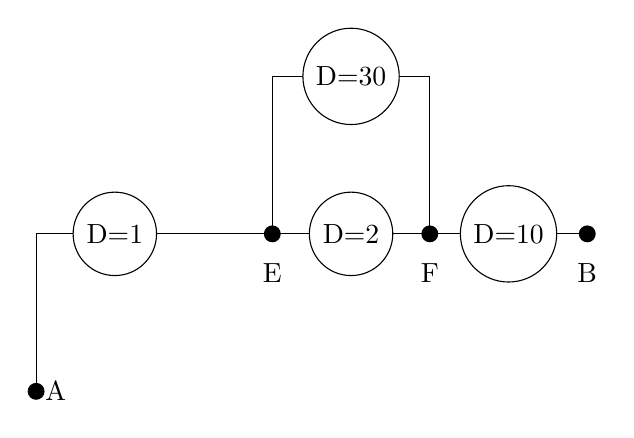
\begin{tikzpicture}
\filldraw (0,-2) circle[radius=1 mm];
\node at (0.25,-2) {A};
\draw (0,-2)--(0,0)--(1,0)node[circle, draw=black,radius=2cm, fill=white]{D=1}
--(3,0); 
\draw (3,0)--(4,0)node[circle, draw=black,radius=2cm, fill=white]{D=2}
--(5,0)--(6,0)node[circle, draw=black,radius=2cm, fill=white]{D=10}
--(7,0);
\draw (3,0)--(3,2)--(4,2)node[circle, draw=black,radius=2cm, fill=white]{D=30}--(5,2)--(5,0);
\filldraw (3,0) circle[radius=1 mm];
\node at (3,-.5) {E};
\filldraw (5,0) circle[radius=1 mm];
\node at (5,-.5) {F};
\filldraw (7,0) circle[radius=1 mm];
\node at (7,-.5) {B};
\end{tikzpicture}
\caption{A Trust Network. The D's  on the edges represent levels of distrust.}
\label{F:3T}
\end{center}
\end{figure}

Suppose person B gets a piece of information indirectly from source A. B gets the information from F but the distrust is rather high. F gets the information from E but by two different channels, one trustworthy and one not. Finally, E gets the information from A via a very trustworthy source (a low distrust level).\par

Examine the information passed from E to F. There are two paths, both saying the same thing. The distrusted path\footnote{Maybe it is a person with low credibility, or maybe newspaper article that had been wet and hard to read.} doesn't matter much, but doesn't hurt either. If anything, the distrusted source slightly increases overall credibility of the information.\par

\begin{blevel}
Calculate the total level of distrust from A to B. Assume parallel combinations of distrust combine the same way as parallel combinations of resistors.
\end{blevel}

\begin{clevel}
Suppose another pathway opened up directly from A to B with a distrust level of 5 (medium). What would be the new total level of distrust from A to B.
\end{clevel}

Of course, we could model the edges according to levels of trust instead of distrust. The level of trust would be the inverse of the level of distrust ($T=\frac{1}{D}$), like the relationship between resistance and conductance. Twice the level of distrust would correspond to half the level of trust. Higher trust leads to a more effective flow of information. The network of Figure~\ref{F:3T} would look like Figure~\ref{F:3T2}.
 
\begin{figure}[H]
\begin{center}
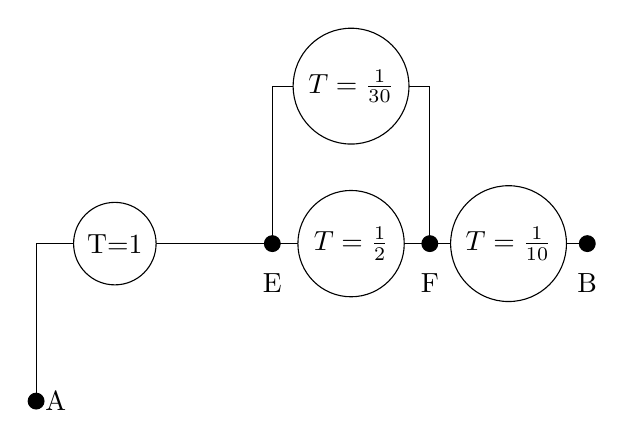
\begin{tikzpicture}
\filldraw (0,-2) circle[radius=1 mm];
\node at (0.25,-2) {A};
\draw (0,-2)--(0,0)--(1,0)node[circle, draw=black,radius=2cm, fill=white]{T=1}
--(3,0); 
\draw (3,0)--(4,0)node[circle, draw=black,radius=2cm, fill=white]{$T=\frac{1}{2}$}
--(5,0)--(6,0)node[circle, draw=black,radius=2cm, fill=white]{$T=\frac{1}{10}$}
--(7,0);
\draw (3,0)--(3,2)--(4,2)node[circle, draw=black,radius=2cm, fill=white]{$T=\frac{1}{30}$}--(5,2)--(5,0);
\filldraw (3,0) circle[radius=1 mm];
\node at (3,-.5) {E};
\filldraw (5,0) circle[radius=1 mm];
\node at (5,-.5) {F};
\filldraw (7,0) circle[radius=1 mm];
\node at (7,-.5) {B};
\end{tikzpicture}
\caption{A Trust Network. The T's represents edges of Trust.}
\label{F:3T2}
\end{center}
\end{figure}

Since trust levels are the inverse of distrust levels, their series and parallel combinations would be as follows:

\begin{align*}
D_T&=D_1+D_2&\rightarrow&\frac{1}{T_T}=\frac{1}{T_1}+\frac{1}{T_2}&\text{Series}\\
\frac{1}{D_T}&=\frac{1}{D_1}+\frac{1}{D_2}&\rightarrow&T_T=T_1+T_2&\text{Parallel}
\end{align*}

Notice that these relationship are exactly reversed from the series and parallel combinations that you get from using levels of distrust.\par

\begin{blevel}
If the units of distrust were Lyes, what would be the units of trust?
\end{blevel}

\begin{clevel}
Calculate the total level of trust from A to B. Is your answer consistent with your previous value of the total level of distrust from A to B?
\end{clevel}

%%%%%%%%%%%%%%%%%%%%%%%%%%%%%%%%%%%%%%%%%%%%%%%%%%%%%%%%%
\subsection{Series and Parallel Combinations of Sources}
Consider two voltage sources connected in series and then in parallel as shown in Figure~\ref{F:3SSP}. In this section, we will see how to simplify combinations of sources.

\begin{figure}[H]
\begin{center}
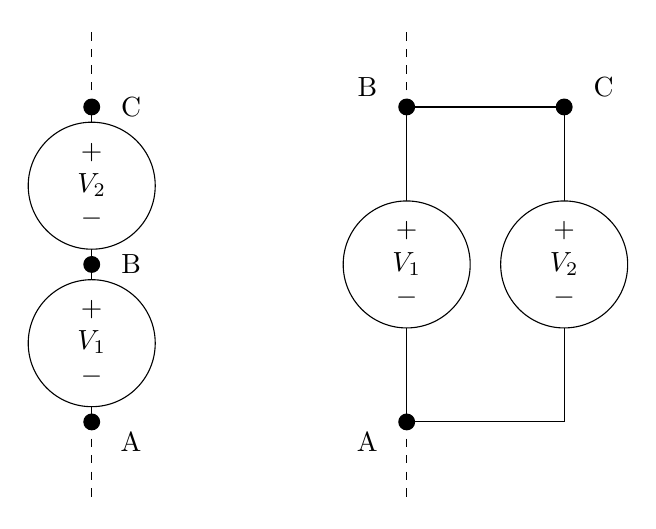
\begin{tikzpicture}
\filldraw (0,0) circle[radius=1 mm]; \draw node at (.5,-.25) {A};
\filldraw (0,2) circle[radius=1 mm]; \draw node at (.5,2) {B};
\filldraw (0,4) circle[radius=1 mm]; \draw node at (.5,4) {C};
\draw (0,0)--(0,1)node[circle, draw=black,radius=2cm, fill=white]{$\begin{matrix}+\\V_1\\-\end{matrix}$}
--(0,2); 
\draw (0,2)--(0,3)node[circle, draw=black,radius=2cm, fill=white]{$\begin{matrix}+\\V_2\\-\end{matrix}$}--(0,4);
\filldraw (4,0) circle[radius=1 mm]; \draw node at (3.5,-.25) {A};
\filldraw (4,4) circle[radius=1 mm]; \draw node at (3.5,4.25) {B};
\filldraw (6,4) circle[radius=1 mm]; \draw node at (6.5,4.25) {C};
\draw (4,0)--(4,2)node[circle, draw=black,radius=2cm, fill=white]{$\begin{matrix}+\\V_1\\-\end{matrix}$}
--(4,4); 
\draw (4,0)--(6,0)--(6,2)node[circle, draw=black,radius=2cm, fill=white]{$\begin{matrix}+\\V_2\\-\end{matrix}$}
--(6,4)--(4,4); 
\draw [dashed] (4,0)--(4,-1);
\draw [dashed] (4,4)--(4,5);
\draw [dashed] (0,0)--(0,-1);
\draw [dashed] (0,4)--(0,5);
\end{tikzpicture}
\caption{Series and Parallel Combinations of Voltage Sources}
\label{F:3SSP}
\end{center}
\end{figure}

Consider first the series combination. Apply KVL. Go around the following loop: start at A, go to B, up to C, then come back through the air \footnote{Some students feel uncomfortable thinking of the air as a legitimate path. Sure, it has a high resistance, but there's nothing wrong with it.} to A. Remember, $V_{BA}$ means $V_B-V_A$. Then:
\begin{align*}
V_{BA}+V_{CB}+V_{AC}&=0\\
V_{CA}=V_{BA}+V_{CB} =V_1+V_2 &=V_{combined}
\end{align*}
Voltage sources in series add.\par

On the other hand, the parallel combination presents the following problems:
\begin{itemize}
\item Apply KVL to the loop starting at A. Go up through $V_1$ to B then down through $V_2$ and then back to A. The sum of these voltages would only be zero if $V_1$ matched $V_2$. Otherwise, KVL is broken. Whoops.
\item Suppose you calculated the current from B to C. 
\begin{align*}
I=\frac{\Delta V}{R}=\frac{V_1-V_2}{0} \rightarrow \infty
\end{align*}
An infinite current\footnote{Mathematically its undefined, but the resistance isn't actually 0, its just small.} is a problem. It would lead to infinite magnetic fields, require more than all the charge in the Universe, etc...
\end{itemize}
Ideal voltage sources of different amounts should not be combined in parallel. Real ones shouldn't either. Real world voltage sources have some internal resistance that would prevent infinite currents and prevent a breakdown of KVL, but they might still overheat or break or cause a fire.

\begin{clevel}
How would two current sources combine in parallel? How about two current sources in series?
\end{clevel}

%%%%%%%%%%%%%%%%%%%%%%%%%%%%%%%%%%%%%%%%%%%%%%%%%%%%%%%%
\section{Application: Two chain saws}
Suppose you and a friend want to cut up some brush. You both have 1.25 hp electric chain saws. You extend a 14-gauge 100' extension cord from the home to the brush and then connect a power strip to the end. You then plug in both chain saws into the power strip. The chain saws are designed to operate at 120V, but will work normally so long as the voltage does not dip below 100V. What is the actual voltage at the chain saw if the outlet provides 115V?
\par
Let's make a model for this situation. We'll leave the third prong wire off the diagram; that wire is needed for safety but won't effect our calculations.\par

Next, we'll make our model as simple as we can, while still hoping to get some useful results. For example, we will model the chainsaw as a resistor, even though it's a little more complicated than that. We will model the extension cord as a perfect wire, but with all of its resistance lumped together as two resistors - one on the way out and one on the way back.

\begin{figure}[H]
\begin{center}
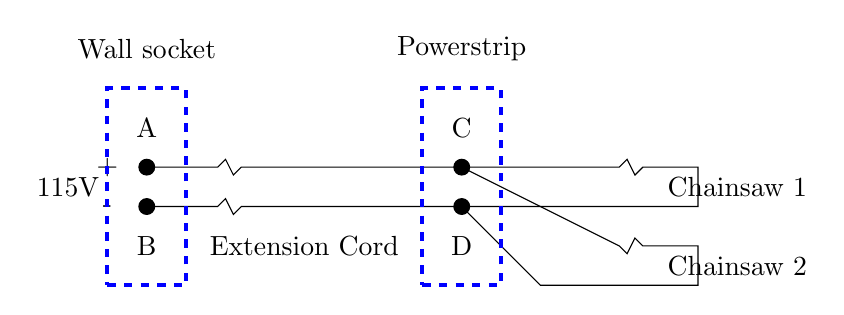
\begin{tikzpicture}
\draw (0,0)--(.9,0)--(1,.1)--(1.1,-.1)--(1.2,0)--(4,0);
\filldraw (4,0) circle[radius=1 mm];
\draw (0,.5)--(.9,.5)--(1,.6)--(1.1,.4)--(1.2,.5)--(4,.5);
\filldraw (4,.5) circle[radius=1 mm];
\draw node at (0,1) {A};
\draw node at (0,-.5) {B};
\draw node at (4,1) {C};
\draw node at (4,-.5) {D};
\draw node at (-.5,0) {-};
\draw node at (-.5,.5) {+};
\draw node at (-1,.25) {115V};
\draw node at (2,-.5) {Extension Cord};
\draw node at (7.5,.25) {Chainsaw 1};
\draw node at (7.5,-.75) {Chainsaw 2};
\filldraw (0,.5) circle[radius=1 mm];
\filldraw (0,0) circle[radius=1 mm];
\draw (4,.5)--(6,.5)--(6.1,.6)--(6.2,.4)--(6.3,.5)--(7,.5)--(7,0)--(4,0);
\draw (4,.5)--(6,-.5)--(6.1,-.6)--(6.2,-.4)--(6.3,-.5)--(7,-.5)--(7,-1)--(5,-1)--(4,0);
\draw [dashed, draw=blue,line width= 0.5mm] (3.5,-1) --(4.5,-1)--(4.5,1.5)--(3.5,1.5)-- (3.5,-1);
\draw node at (4,2) {Powerstrip};
\draw [dashed, draw=blue,line width= 0.5mm] (-.5,-1) --(.5,-1)--(.5,1.5)--(-.5,1.5)-- (-.5,-1);
\draw node at (0,2) {Wall socket};
\end{tikzpicture}
\caption{Electrical model of two chainsaws plugged into a power strip}
\end{center}
\end{figure}

Nodes A and B are at the outlet. Nodes C and D are at the power strip somewhere in the backyard or alley.

\par
We need to determine the resistance values for the extension cord and chainsaw models. Look up the cross-sectional area of a 14-gauge wire and the resistivity of copper.
\par
\begin{align*}
R_{cord} &= \rho \frac{L}{A}\\
R_{cord}&=(1.68E-8) \Omega m \frac{30.48 m}{(2.08E-6) m^2} = 0.246 \Omega
\end{align*}

\begin{blevel}
Based on the values used in the above equation, is this extension cord made of copper or aluminum. How can you tell? 
\end{blevel}

To approximate the resistance of the chainsaws \footnote{The electric chainsaw would be more accurately modeled as a series resistor-inductor combination, but we won't cover inductors until later in the book.}, we'll use the expected chainsaw power value, which is specified at ~120V to determine the current. Then, use values of the current and voltage and Ohm's Law to determine the resistance.
\par

\begin{align*}
P&=IV\\
1.25hp*745 \frac{Watts}{hp}&= I*120 \rightarrow I=7.8 Amps\\
V &= IR \\
120 &= 7.8*R \rightarrow R = 15.46 \Omega
\end{align*}

Now, we'll use our analysis tools to determine the voltage across the chainsaws.

\begin{enumerate}
\item Combine the two chainsaw resistances. Observe that they are in parallel. $R_{combined} = 7.73 \Omega$
\item The combined chainsaw resistance connects in series with the two extension cords resistances. Combining these gives one total resistance of $R_T=8.22 \Omega$
\item Use Ohm's Law to determine the current entering the positive wire of the extension cord. I = 13.99 A.
\item Go back to the unsimplified circuit and use Ohm's Law to determine the voltage drop across the two legs of the extension cord. $V_{cordLeg} =3.44 V$
\item Use KVL to determine the voltage drop across one of the chainsaws. $+115V - 3.44 - V_{saw} - 3.44 = 0$. So, $V_{saw}=108.1 V$ 
\item Conclusion: The voltage does not dip below 100V, so the chainsaws should be OK.
\end{enumerate}

\begin{blevel}
Suppose a third chainsaw were plugged into the power strip. What would the voltage be across each operating chainsaw?
\end{blevel}

\begin{clevel}
What is the combined resistance of N identical resistors connected in parallel?
\end{clevel}

\begin{clevel}
Suppose N chainsaws were plugged into the power strip. Each chainsaw using 1.25 hp of power, and the 14-gauge copper extension cord is still 100 feet long. Determine the voltage across each chainsaw in terms of N.
\end{clevel}

\subsection{Series and Parallel: Springs}
To reinforce the two big ideas of this section (simplification and the generality of series/parallel combinations), we will examine a combination of springs. Consider the network shown below:
\begin{figure}[H]
\begin{center}
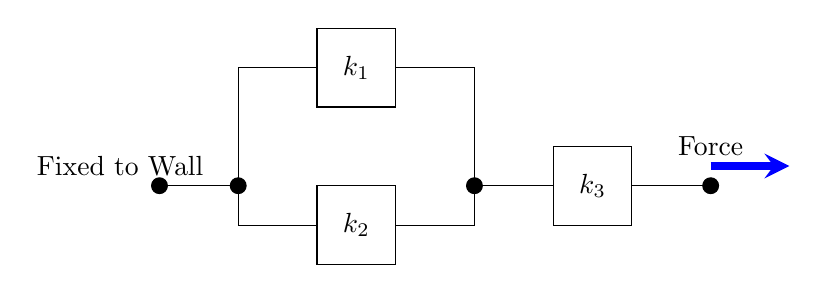
\begin{tikzpicture}
\draw [draw=black] (1,2) rectangle  (2,3); \draw node at (1.5,2.5) {$k_1$};
\draw [draw=black] (1,0) rectangle  (2,1); \draw node at (1.5,0.5) {$k_2$};
\draw [draw=black] (4,.5) rectangle  (5,1.5); \draw node at (4.5,1) {$k_3$};
\filldraw (0,1) circle[radius=1 mm];
\draw (-1,1)--(0,1)--(0,2.5)--(1,2.5) (0,1)--(0,.5)--(1,.5);
\filldraw (3,1) circle[radius=1 mm];
\draw (2,.5)--(3,.5)--(3,2.5)--(2,2.5) (3,1)--(4,1) (5,1)--(6,1);
\filldraw (6,1) circle[radius=1 mm];
\filldraw (-1,1) circle[radius=1 mm];
\draw node at (-1.5,1.25) {Fixed to Wall};
\draw node at (6,1.5) {Force};
\draw [draw=blue, line width=1 mm][-stealth] (6,1.25)--(7,1.25);
\end{tikzpicture}
\caption{A mechanical network of springs.}
\end{center}
\end{figure}

Can we compactly describe this network of springs? Yes: $k_1 \parallel k_2+k_3$. Can we replace this combination with one equivalent spring? Yes, but we need to do just a little thinking. First, we write the ideal spring relationship (called Hooke's Law).

\begin{align*}
F=-k\Delta x&&\text{Hooke's Law}
\end{align*}

We'll call `k' the spring constant. A stiffer spring would have a larger k\footnote{We just as easily could have used $F=-\frac{\Delta x}{C}$, where C is the compliance or looseness of the spring. A higher C would mean lower stiffness. Not surprising, if we did this, the series and parallel relationships would be reversed.}.

\begin{alevel}Suppose a 10N force is applied to $k_3$. Determine the amount that it stretches.\end{alevel}

For a parallel combination of two springs, the forces on each spring must sum to the total force applied, but the amount of stretch must be the same for the two springs and their equivalent.

\begin{align*}
F_T&=F_1+F_2&&\text{Forces must add}\\
k_T\Delta x &= k_1\Delta x+k_2\Delta x&&\text{Use Hooke's Law}\\
k_T &= k_1+k_2&&
\end{align*}
Conclusion. Spring constants add in parallel. 

\begin{clevel}Prove that for springs in series that: $\frac{1}{k_T}=\frac{1}{k_1}+\frac{1}{k_2}$.\end{clevel}.

\begin{blevel}If $k_1=5 \frac{N}{m}$, $k_2=2 \frac{N}{m}$, and $k_3=10 \frac{N}{m}$, then determine the equivalent spring constant of the system. Also determine the amount that this network would stretch if a 3 Newton force were applied as shown. \end{blevel}


\subsection{Series and Parallel: Tasks}
To \emph{further} reinforce the two big ideas of this section (simplification and the generality of series/parallel combinations), we examine a network of tasks. Consider a job that takes two steps (A and B) where each task must be completed one after the next (series). The first job can be accomplished by two workers working side by side (parallel). \par
Worker 3 takes time $T_{3B}$ hours to complete job B. Worker 2 takes time $T_{2A}$ hours to complete that part of the job if working alone. Worker 1 takes time $T_{1A}$ hours to complete job A if working alone. This task network can be drawn as shown:

\begin{figure}[H]
\begin{center}
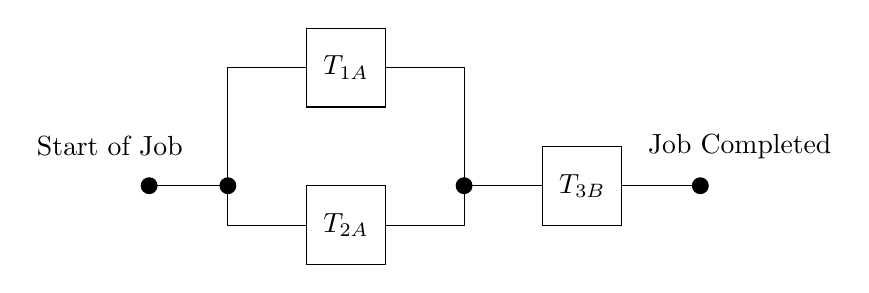
\begin{tikzpicture}
\draw [draw=black] (1,2) rectangle  (2,3); \draw node at (1.5,2.5) {$T_{1A}$};
\draw [draw=black] (1,0) rectangle  (2,1); \draw node at (1.5,0.5) {$T_{2A}$};
\draw [draw=black] (4,.5) rectangle  (5,1.5); \draw node at (4.5,1) {$T_{3B}$};
\filldraw (0,1) circle[radius=1 mm];
\draw (-1,1)--(0,1)--(0,2.5)--(1,2.5) (0,1)--(0,.5)--(1,.5);
\filldraw (3,1) circle[radius=1 mm];
\draw (2,.5)--(3,.5)--(3,2.5)--(2,2.5) (3,1)--(4,1) (5,1)--(6,1);
\filldraw (6,1) circle[radius=1 mm];
\filldraw (-1,1) circle[radius=1 mm];
\draw node at (-1.5,1.5) {Start of Job};
\draw node at (6.5,1.5) {Job Completed};
\end{tikzpicture}
\label{F3:JOBS}
\caption{A network of tasks.}
\end{center}
\end{figure}

Next we try to develop some rules for combining times where the work is done in series and then in parallel. If in series the times would add:

\begin{align*}
T_{Total}=T_1+T_2
\end{align*}

Before studying the parallel case, it might be more useful to think in terms of the rate that work is completed. The time to complete the work has units of hours per job. The rate would be completed jobs per hour. Thus the rate and time would be inverses of each other ($R=\frac{1}{T}$).\par
If two worker work in parallel, the rates that the work is done would add because they are both contributing towards the completion of the project.

\begin{align*}
R_{Total}&=R_1+R_2\\
\frac{1}{T_{Total}}&=\frac{1}{T_1}+\frac{1}{T_2}
\end{align*}

\begin{blevel}
For the project shown in Figure~\ref{F3:JOBS}, suppose it would take 3 hours for worker 1 to complete job A alone and 5 hours for worker 2 to complete job A alone and 6 hours for worker 3 to complete job B alone. How much time will it take to complete the entire project?
\end{blevel}

\begin{blevel}
X can mow a lawn in 5 hours and Y can mow the same lawn in 9 hours and Z and mow the same lawn in 11 hours. How long will it take to mow the lawn if they are all working together?
\end{blevel}


%%%%%%%%%%%%%%%%%%%%%%%%%%%%%%%%%%%%%%%%%%%%%%%%%%%%%%%%%%%%
\section{Voltage Division}
We have established some basic tools, but now it might be worthwhile to look at a common situation in detail. This situation occurs often, so we want to be quick with its analysis.
\par
The situation involves two resistors connected in series.
\par
\begin{figure}[H]
\begin{center}
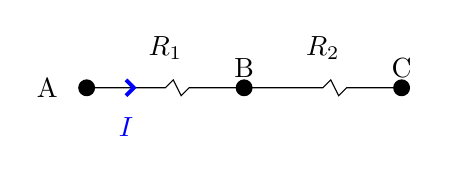
\begin{tikzpicture}
\node at (2,.5) {$R_1$};
\node at (4,.5) {$R_2$};
\filldraw (1,0) circle[radius=1 mm];
\node at (.5,0) {A};
\filldraw (3,0) circle[radius=1 mm];
\node at (3,.25) {B};
\filldraw (5,0) circle[radius=1 mm];
\node at (5,.25) {C};
\draw (1,0)--(2,0)--(2.1,.1)--(2.2,-.1)--(2.3,0)--(3,0);
\draw (3,0)--(4,0)--(4.1,.1)--(4.2,-.1)--(4.3,0)--(5,0);
\draw [draw=blue, line width=0.5mm] (1.5,.1)--(1.6,0)--(1.5,-.1);
\node [text=blue] at (1.5,-.5) {$I$};
\end{tikzpicture}
\caption{The basic voltage division situation}
\end{center}
\end{figure}

Imagine going around a loop where we start at A, go around through the air to C, then from C to B and then from B back to A. KVL says that the total voltage drop around this loop must be zero.
\par
\begin{align*}
V_{AC} + V_{CB}+V_{BA}&=0\\
V_{AC} &=-V_{CB}-V_{BA}\\
V_{AC} &= V_{AB}+V_{BC} \tag{Individual Voltages Sum to Total Voltage}\\
\end{align*}

Solve for $I$. 

\begin{align*}
V_{AC} &= V_{AB}+V_{BC}\\
V_{AC} &= IR_1+IR_2 \rightarrow I=\frac{V_{AC}}{R_1+R_2}
\end{align*}

Then find voltage across $R_1$, called $V_{AB}$:

\begin{align}
V_{AB}&=IR_1\notag\\
V_{AB}&=\frac{V_{AC}}{R_1+R_2}R_1\notag\\
V_{AB}&=\frac{R_1}{R_1+R_2}V_{AC}
\end{align}

We conclude that a fraction ($\frac{R_1}{R_1+R_2}$) of the total voltage is dropped across $R_1$, and that fraction is the same as the fraction of the total series resistance that is $R_1$.
\par


\begin{alevel}
Suppose $V_{AC}$ were 18 V and $R_1$ were 5 $\Omega$ and $R_2$ were 10 $\Omega$. How much voltage would be dropped across $R_1$? What about $R_2$?
\end{alevel}

\begin{blevel}
Suppose $V_{AC}$ were 18 V and $R_1$ were 5 $\Omega$ and $R_2$ were 10 $\Omega$.\\
What is $V_{AB}+V_{BC}$?\\
What is $V_{AB}+V_{BA}$?\\
What is $V_{AB}+V_{CB}$?
\end{blevel}

\begin{dlevel}
Prove that for N resistors in series, the voltage drop across $R_i$ is:
\par
\[ V_i=\frac{R_i}{(\sum\limits_{j=1}^{j=N} R_j)}V_{TOTAL} \]
\end{dlevel}

Consider a more complicated circuit like that shown in Figure~\ref{F:3VD}. Use voltage division to find the voltage across the 2 Ohm ($V_2$)resistor as follows:

\begin{enumerate}
\item Determine the fraction that $V_2$ is of $V_{BC}$. Answer: $V_2=\frac{2}{2+3}V_{BC}$
\item Determine the fraction that $V_{BC}$ is of $V_{AC}$. Answer: $V_{BC}=\frac{R_{BC}}{R_{BC}+5}V_{AC}$
\item Identify $R_{BC} = (2+3) \parallel 7$ $\Omega$
\item String it all together: 
\begin{align}
V_2=(\frac{2}{2+3})(\frac{(2+3) \parallel 7}{(2+3) \parallel 7+5})V_{AC}
\end{align}
\end{enumerate}

\par
\begin{figure}[H]
\begin{center}
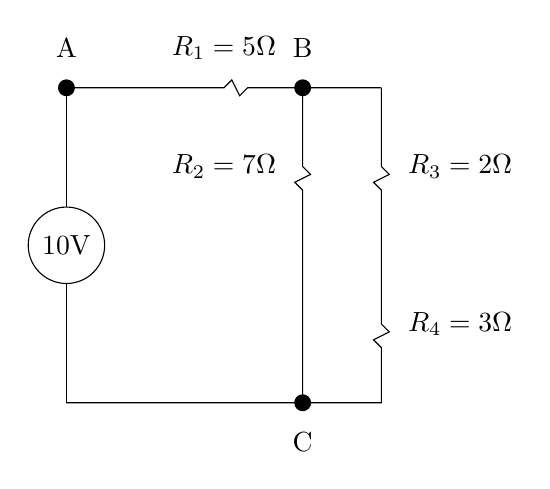
\begin{tikzpicture}
\node at (2,4.5) {$R_1=5\Omega$};
\node at (2,3) {$R_2=7\Omega$};
\node at (5,3) {$R_3=2\Omega$};
\node at (5,1) {$R_4=3\Omega$};
\filldraw (0,4) circle[radius=1 mm];
\node at (0,4.5) {A};
\filldraw (3,4) circle[radius=1 mm];
\node at (3,4.5) {B};
\filldraw (3,0) circle[radius=1 mm];
\node at (3,-.5) {C};
\draw (0,0)--(0,2) node[circle, draw=black, fill=white] {10V}--(0,4);
\draw (0,4)--(2,4)--(2.1,4.1)--(2.2,3.9)--(2.3,4)--(3,4)--(4,4);
\draw (4,4)--(4,3)--(4.1,2.9)--(3.9,2.8)--(4,2.7)--(4,2)
--(4,1)--(4.1,.9)--(3.9,.8)--(4,.7)--(4,0)--(0,0);
\draw (3,4)--(3,3)--(3.1,2.9)--(2.9,2.8)--(3,2.7)--(3,0);
\end{tikzpicture}
\caption{Circuit for practicing voltage division.}
\label{F:3VD}
\end{center}
\end{figure}

\begin{blevel}
Finish the calculation and get a value for the voltage across the 2 Ohm resistor. What is the current through it? 
\end{blevel}

\begin{clevel}
Use voltage division to determine the voltage across the 7 Ohm resistor in Figure~\ref{F:3VD}. 
\end{clevel}

\begin{clevel}
Use voltage division to determine the voltage across the 3 Ohm resistor in Figure~\ref{F:3VD}. 
\end{clevel}
%%%%%%%%%%%%%%%%%%%%%%%%%%%%%%%%%%%%%%%%%%%%%%%%%%%%%%%%%%%%%%%%%

%%%%%%%%%%%%%%%%%%%%%%%%%%%%%%%%%%%%%%%%%%%%%%%%%%%%%%%%%%%%%%%%

\chapter{Analyzing DC Circuits - Powerful Tools}

Electrical networks can be complicated. One might model a computer chip as an electrical network containing millions or billions of nodes and edges. In this chapter, we further develop our analysis tools to be able to handle more complicated circuits.
\par
The first two sections introduce algorithms that you, or a computer, could use to analyze a circuit. The third technique involves combining sources to simplify an otherwise complex circuit, while hopefully providing some intuitive insight about voltage and current sources. The fourth technique, superposition, transcends several engineering classes and will provide further insight into linear circuits, and engineering systems.
\par
\section{Nodal Analysis}
This section describes a method of analysis called Nodal Analysis. The basic strategy of this technique is to:
\begin{itemize}
\item Identify uniques nodes.
\item Create a variable to represent the voltage difference for each node with respect to a common reference point. For node A, this will be called $V_{A-Ref}$ or just shortened to $V_A$.
\item For each node write down $\Sigma I_{in}=0$. 
\end{itemize}

\subsection{Simple Example}
Let's try out this procedure for a simple example and work out the bugs.

\begin{figure}[H]
\begin{center}
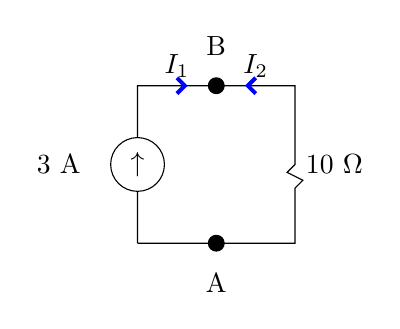
\begin{tikzpicture}
\draw (0,0)--(0,1)node[circle, draw=black, fill=white]{$\uparrow$}--(0,2)--(2,2)
--(2,1)--(1.9,.9)--(2.1,.8)--(2,.7)--(2,0)--(0,0);
\draw node at (-1,1) {3 A};
\draw node at (2.5,1) {10 $\Omega$};
\draw node at (1,2.5) {B};
\draw node at (1,-.5) {A};
\filldraw (1,2) circle[radius=1 mm];
\filldraw (1,0) circle[radius=1 mm];
\draw [draw=blue, line width=0.5mm] (.5,2.1)--(.6,2)--(.5,1.9);
\draw node at (.5,2.25) {$I_1$};
\draw [draw=blue, line width=0.5mm] (1.5,2.1)--(1.4,2)--(1.5,1.9);
\draw node at (1.5,2.25) {$I_2$};
\end{tikzpicture}
\caption{A simple nodal analysis example}
\end{center}
\end{figure}

Write $\Sigma I_{in}=0$ for each node. We have two nodes. We'll need to determine the current through resistors. Ohm's Law says that the current is the voltage \textbf{difference} across the resistor divided by the resistance. 
\par
\begin{align}
I_1+I_2=0 \rightarrow 3 + \frac{A-B}{10}=0&&\text{Node B} \label{E:4N}\\
-I_1-I_2=0 \rightarrow -3 + \frac{B-A}{10}=0&&\text{Node A} \notag 
\end{align} 

So far, so good - we have two equations and two unknowns. Our system of two equations looks like it should produce one solution. But look closely at the second equation, it is just the first equation multiplied by (-1)! The second equation is a duplicate of the first.\par

We really just have one equation and two unknowns. We would say that these two equations are not independant.\par

\begin{alevel}
Consider the following set of N equations and M unknowns. What are M and N?
\begin{align*}
3x+y&=10\\
x-y&=5\\
2x-5y&=8
\end{align*} 
\end{alevel}

\begin{blevel}
If you have one equation and two unknowns, how many solutions will you have? One? Infinite? None?
\end{blevel}

\begin{clevel}
Solve the following equation for x and y: (x+y=10). Report ALL solutions.
\end{clevel}

\begin{dlevel}
Suppose you have three equations and three unknowns. How can you tell if the third equation is just a combination of the other two?
\end{dlevel}

Let's continue with our example and solve for all possible combinations for the voltages at A and B.
\par
\begin{align*}
3 + \frac{A-B}{10}=0\tag{Node B}\\
30 = B-A\\
B = A+30&&\leftarrow \text{rearranged Node B equation}
\end{align*} 

So, A can be anything so long as B is 30V higher than A. Figure~\ref{F:4NS} shows some of the possible solutions:

\begin{figure}[H]
\begin{center}
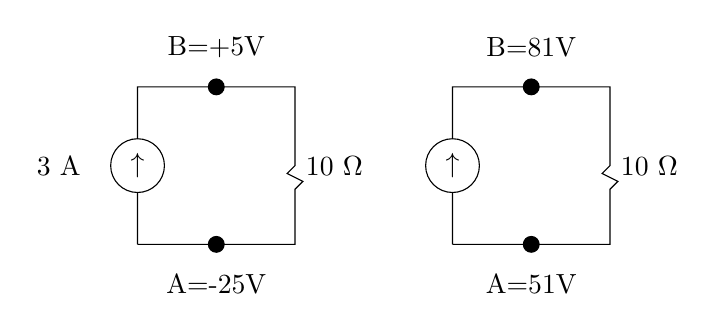
\begin{tikzpicture}
\draw (0,0)--(0,1)node[circle, draw=black, fill=white]{$\uparrow$}--(0,2)--(2,2)
--(2,1)--(1.9,.9)--(2.1,.8)--(2,.7)--(2,0)--(0,0);
\draw node at (-1,1) {3 A};
\draw node at (2.5,1) {10 $\Omega$};
\draw node at (1,2.5) {B=+5V};
\draw node at (1,-.5) {A=-25V};
\filldraw (1,2) circle[radius=1 mm];
\filldraw (1,0) circle[radius=1 mm];
%
\draw (4,0)--(4,1)node[circle, draw=black, fill=white]{$\uparrow$}--(4,2)--(6,2)
--(6,1)--(5.9,.9)--(6.1,.8)--(6,.7)--(6,0)--(4,0);
\draw node at (6.5,1) {10 $\Omega$};
\draw node at (5,2.5) {B=81V};
\draw node at (5,-.5) {A=51V};
\filldraw (5,2) circle[radius=1 mm];
\filldraw (5,0) circle[radius=1 mm];
\end{tikzpicture}
\caption{Two possible solutions for node voltages that satisfy Equation~\ref{E:4N}}
\label{F:4NS}
\end{center}
\end{figure}

Both are correct. There are an infinite number of solutions, but all solutions agree that the voltage DIFFERENCE from B to A is 30V.
\par
We can simplify things by requiring that we only present one of these solutions, one where one of the nodes is set to zero. In order words, we'll pick one of the nodes as the voltage reference point. Let's pick node A=0. Mathematically, this adds another equation (A=0). Our set of equations now looks like this:

\begin{align}
3 + \frac{A-B}{10}&=0\tag{Node B}\\
A&=0 \tag{Assign reference node}
\end{align} 

These equations are independent. Two independant equations with two variables leads to one solution. It wouldn't be hard to find a solution by substitution, but let's put the system of equations into matrix form and solve it that way. The matrix method works well when we have larger numbers of equations and unknowns.

\begin{align*}
\frac{1}{10}A-\frac{1}{10}B&=-3\\
A+0*B&=0
\end{align*}

\begin{align}
\left[ \begin{matrix}
\frac{1}{10} &	-\frac{1}{10}\\
1		&	0 \\
\end{matrix} \right]
\left[ \begin{matrix}
A\\
B\\
\end{matrix} \right]
=
\left[ \begin{matrix}
-3\\
0\\
\end{matrix} \right] \notag \\
M\vec{z}=\vec{b}
\end{align} 

Where M represesnts a 2x2 matrix\footnote{We usually employ the capitol letter A for this matrix, but because is one of the variables, I'm using M instead.}, z is the variable (with two parts, A and B), and b is the numerical term. To solve, find the inverse matrix for M and then apply it to both sides of the equation.

\begin{align}
M^{-1}M\vec{z}=M^{-1}\vec{b} \notag\\
\vec{z} = M^{-1}\vec{b}
\end{align} 

$M^{-1}$ can be found using a little linear algebra, google sheets, Matlab, or one of many other computational tools. In our case $M^{-1}$ turns out to be:


\begin{align*}
M^{-1}=\left[ \begin{matrix}
0 &	1\\
-10		&	1 \\
\end{matrix} \right]
\end{align*} 

\begin{blevel}
Multiply $M^{-1}$ by $\vec{b}$ to determine values for A and B. If you aren't familiar with matrix multiplication, look it up.
\end{blevel}

\begin{blevel}
The identity matrix, I, has all ones along the diagonal. Consider the 2x2 identity matrix multiplied by another generic 2x2 matrix as shown below. What do you get?

\begin{align*}
\left[ \begin{matrix}
1 &	0\\
0&	1 \\
\end{matrix} \right]*\left[ \begin{matrix}
a &	b\\
c&	d \\
\end{matrix} \right]=?
\end{align*} 
\end{blevel}

\begin{blevel}
Simplify $I^{5}$.
\end{blevel}

\begin{blevel}
Multiply $M^{-1}$ by M and see what you get. What this expected?
\end{blevel}

\begin{blevel}
Multiply $(M^{-1})^4$ by $M^5$. What do you get?
\end{blevel}

\begin{blevel}
Multiply this out:
\begin{align*}
\begin{vmatrix}0 &	1&2\\-10&1	&1 \\\end{vmatrix}
\begin{vmatrix}0 &	1\\-10&1\\ 2&3\\ \end{vmatrix}
\end{align*}
\end{blevel}

\begin{clevel}
When multiplying matrices together, there is a size rule. For example, you can multiply a 3x2 by a 2x7 matrix, but not a 2x7 by a 3x2. Describe the rule that determines if two matrices can be multiplied together?
\end{clevel}

\subsection{A more complex example}
Let's apply Nodal Analysis to a more complex problem.
\par
\begin{figure}[H]
\begin{center}
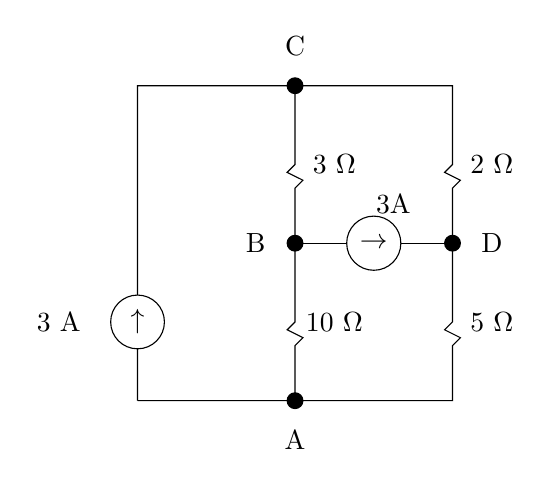
\begin{tikzpicture}
\draw (0,0)--(0,1)node[circle, draw=black, fill=white]{$\uparrow$}--(0,4)--(2,4)--(2,3)
--(1.9,2.9)--(2.1,2.8)--(2,2.7)--(2,2)--(2,1)
--(1.9,.9)--(2.1,.8)--(2,.7)--(2,0)--(0,0);
\draw (2,4)--(4,4)--(4,3)
--(3.9,2.9)--(4.1,2.8)--(4,2.7)--(4,2);
\draw (2,2)--(3,2)node[circle, draw=black, fill=white]{$\rightarrow$}--(4,2);
\draw node at (3.25,2.5) {3A};
\draw (4,2)--(4,1)
--(3.9,.9)--(4.1,.8)--(4,.7)--(4,0)--(2,0);
\draw node at (-1,1) {3 A};
\draw node at (2.5,1) {10 $\Omega$};
\draw node at (4.5,1) {5 $\Omega$};
\draw node at (2.5,3) {3 $\Omega$};
\draw node at (4.5,3) {2 $\Omega$};
\draw node at (1.5,2) {B};
\draw node at (2,-.5) {A};
\draw node at (2,4.5) {C};
\draw node at (4.5,2) {D};
\filldraw (2,4) circle[radius=1 mm];
\filldraw (2,2) circle[radius=1 mm];
\filldraw (4,2) circle[radius=1 mm];
\filldraw (2,0) circle[radius=1 mm];
\end{tikzpicture}
\caption{More complicated circuit for nodal analysis.}
\end{center}
\end{figure}

Let's make some observations:
\begin{enumerate}
\item There are four nodes, so we could write $\Sigma I_{in}=0$ four times. The last node, however, would not yield an independent equation. It would be a combination of the other three. We'll check that in a minute.

\item We will assign one node to be the reference node. Let's pick A.

\item We have four unknown node voltages (A,B,C and D) but since (A=0), we really only have three unknowns along with three meaningful (independent) node equations, plus $V_A=0$. We can count this as four unknown voltages and four unknown equations, or three equations and three unknowns if we just set A to 0.

\item After we write the equations, we move them into matrix form and solve.
\end{enumerate}

Writing the node equations:
\par
\begin{align}
\frac{C-B}{3}+\frac{0-B}{10}-3=0 &&\text{Node B}\notag\\
3 + \frac{B-C}{3}+\frac{D-C}{2}=0 &&\text{Node C}\notag\\
\frac{C-D}{2}+3+\frac{0-D}{5}=0 &&\text{Node D}
\end{align} 

Then, in matrix form:
\begin{align}
\left[ \begin{matrix}
(-\frac{1}{3}-\frac{1}{10})&	\frac{1}{3}&	0\\
\frac{1}{3}&	(-\frac{1}{3}-\frac{1}{2})&\frac{1}{2}\\
0	&	\frac{1}{2}&	(-\frac{1}{2}-\frac{1}{5})\\
\end{matrix} \right]
\left[ \begin{matrix}
B\\
C\\
D\\
\end{matrix} \right] =
\left[ \begin{matrix}
3\\
-3\\
-3\\
\end{matrix} \right]
\end{align}

\begin{blevel}
Determine $M^{-1}$ for this example.
\end{blevel}

\begin{clevel}
Determine the voltages B, C and D.
\end{clevel}

\begin{blevel}
Use your voltages for B and C to determine the current through the 3 Ohm resistor. Determine the power absorbed by the 3 Ohm resistor.
\end{blevel}

\begin{clevel}
Fill in the table indicating the power absorbed or produced by each component. Check that the power produced by the sources equals the power absorbed by the resistors. Remember, if current flows from - to + for a component, then that component is producing power.
\begin{table}[H]
\begin{center}
\begin{tabular}{|c|c|c|c|} \hline
component & I&$\Delta V$&power absorbed (- if produced) \\ \hline
3 $\Omega$ &&&	\\ \hline
2 $\Omega$&&&	\\ \hline
10 $\Omega$ &&&	\\ \hline
5 $\Omega$ &&&	\\ \hline
3A left source &&&	\\ \hline
3A center source &&&	\\ \hline
\end{tabular}
\caption{Power check}
\label{T:4PCheck}
\end{center}
\end{table}
\end{clevel}

\begin{clevel}
Suppose all the resistors were 10 $\Omega$. Adjust your matrix and redetermine the voltages B, C and D. If you only record your new values for B, C and D, that will be sufficient.
\end{clevel}

%%%%%%%%%%%%%%%%%%%%%%%%%%%%%%%%%%%%%%%%%%%%%%%%%%%%%%
\subsection{Nodal Analysis with a Voltage Source}
Now suppose we swap out one of the current sources for a voltage source as shown in Figure~\ref{F:4NODV}. This complicates things because we no longer know the current flowing from A to D.

\begin{figure}[H]
\begin{center}
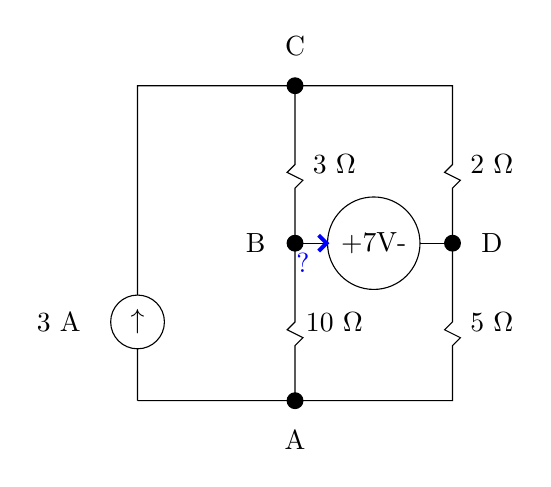
\begin{tikzpicture}
\draw (0,0)--(0,1)node[circle, draw=black, fill=white]{$\uparrow$}--(0,4)--(2,4)--(2,3)
--(1.9,2.9)--(2.1,2.8)--(2,2.7)--(2,2)--(2,1)
--(1.9,.9)--(2.1,.8)--(2,.7)--(2,0)--(0,0);
\draw (2,4)--(4,4)--(4,3)
--(3.9,2.9)--(4.1,2.8)--(4,2.7)--(4,2);
\draw (2,2)--(3,2)node[circle, draw=black, fill=white]{+7V-}--(4,2);
\draw [draw=blue, line width=0.5mm] (2.3,2.1)--(2.4,2)--(2.3,1.9);
\draw [text=blue] node at (2.1,1.75) {?};
\draw (4,2)--(4,1)
--(3.9,.9)--(4.1,.8)--(4,.7)--(4,0)--(2,0);
\draw node at (-1,1) {3 A};
\draw node at (2.5,1) {10 $\Omega$};
\draw node at (4.5,1) {5 $\Omega$};
\draw node at (2.5,3) {3 $\Omega$};
\draw node at (4.5,3) {2 $\Omega$};
\draw node at (1.5,2) {B};
\draw node at (2,-.5) {A};
\draw node at (2,4.5) {C};
\draw node at (4.5,2) {D};
\filldraw (2,4) circle[radius=1 mm];
\filldraw (2,2) circle[radius=1 mm];
\filldraw (4,2) circle[radius=1 mm];
\filldraw (2,0) circle[radius=1 mm];
\end{tikzpicture}
\caption{Current source replaced with voltage source. The current is no longer known.}
\label{F:4NODV}
\end{center}
\end{figure}

We can handle this unknown current by introducing a variable for this unknown current,\footnote{There are other approaches. One approach uses something called supernodes. We might cover it in class, or you might look it up if interested.} call it $I_1$.  Because we introduced another unknown, we need another equation (a bonus equation, if you will). \par
This bonus equation must take into account the information about the voltage source that hasn't yet been considered. The voltage source forces node B to be 7V greater than node D, or $B =D+7$.\par
Our equations look like this:
\
\begin{align}
\frac{C-B}{3}+\frac{0-B}{10}-I_1=0 \tag{Node B}\\
3 + \frac{B-C}{3}+\frac{D-C}{2}=0 \tag{Node C}\\
\frac{C-D}{2}+I_1+\frac{0-D}{5}=0 \tag{Node D}\\
B=D+7 \tag{Bonus Equation due to 7V Voltage Source}
\end{align} 

\begin{clevel}
Put this in matrix form and solve for the voltages at B, C and D. Just answers are sufficient.
\end{clevel}

\begin{alevel}
When doing nodal analysis, is it easier to handle a current source or a voltage source?
\end{alevel}

\begin{clevel}
Replace the other 3A current source with a 3V voltage source (positive side on top). Adjust your analysis accordingly. Write down the new matrix formulation and solve for the voltages at B, C and D.
\end{clevel}

\begin{clevel}
A circuit has 3 voltage sources and 9 nodes. If you follow the above approach, how many rows will the matrix M have?
\end{clevel}

\begin{clevel}
A circuit has 3 voltage sources, 5 current sources and 25 nodes. If you follow the above approach, how many rows will the matrix M have?
\end{clevel}


%%%%%%%%%%%%%%%%%%%%%%%%%%%%%%%%%%%%%%%%%%%%%%%%%%%%%%%%%%%%%%%%%%
\section{Loop Analysis}
Loop analysis is an alternative to nodal analysis. It is based on the idea that the sum of the voltages around any loop add to zero. Sometimes loop analysis is slower, sometimes faster. Sometimes it's more intuitive, sometimes not. It's good to have both tools, just like it pays to have multiple driving routes to your home. If one route closes or has bad weather, you can try the other one.\\

The premise behind loop analysis is to write KVL \footnote{The sum of the voltages around a loop is zero.} for \emph{some} of the loops in the circuit. If we pick the loops carefully, we can avoid duplicate equations and arrive with a solvable set of independent equations.
\par
Our first step is to consider how many loops a circuit might have.
\begin{alevel}
How many rectangles can be found in Figure~\ref{F:4RECT}?
\end{alevel}

\begin{blevel}
How many polygons can be found in Figure~\ref{F:4RECT}?
\end{blevel}

\begin{clevel}
How many polygons \textbf{that do not have any smaller polygons inside them} can be found in Figure~\ref{F:4RECT}?
\end{clevel}

\begin{figure}[H]
\begin{center}
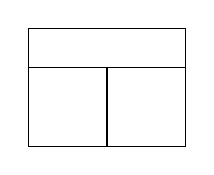
\begin{tikzpicture}
\draw (0,0)--(0,1.5)--(2,1.5)--(2,0)--(0,0);
\draw (0,1)--(2,1) (1,1)--(1,0);
\end{tikzpicture}
\caption{Fun box problem.}
\label{F:4RECT}
\end{center}
\end{figure}

Figure~\ref{F:4R} shows an electric circuit that is similar in structure to Figure~\ref{F:4RECT} (rotated 90 degrees).

\begin{figure}[H]
\begin{center}
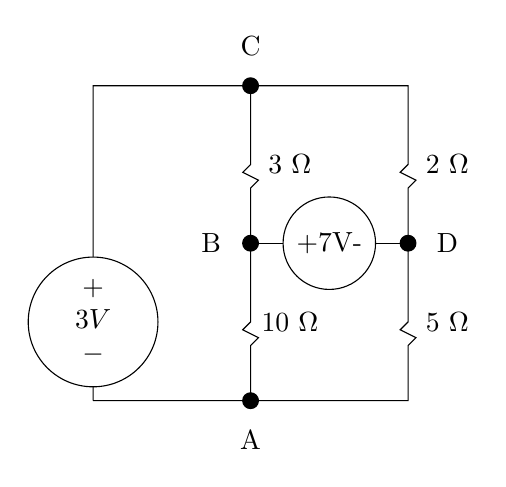
\begin{tikzpicture}
\draw (0,0)--(0,1)node[circle, draw=black, fill=white]{$\begin{matrix}+\\3V\\-\end{matrix}$}--(0,4)--(2,4)--(2,3)
--(1.9,2.9)--(2.1,2.8)--(2,2.7)--(2,2)--(2,1)
--(1.9,.9)--(2.1,.8)--(2,.7)--(2,0)--(0,0);
\draw (2,4)--(4,4)--(4,3)
--(3.9,2.9)--(4.1,2.8)--(4,2.7)--(4,2);
\draw (2,2)--(3,2)node[circle, draw=black, fill=white]{+7V-}--(4,2);
\draw (4,2)--(4,1)
--(3.9,.9)--(4.1,.8)--(4,.7)--(4,0)--(2,0);
\draw node at (2.5,1) {10 $\Omega$};
\draw node at (4.5,1) {5 $\Omega$};
\draw node at (2.5,3) {3 $\Omega$};
\draw node at (4.5,3) {2 $\Omega$};
\draw node at (1.5,2) {B};
\draw node at (2,-.5) {A};
\draw node at (2,4.5) {C};
\draw node at (4.5,2) {D};
\filldraw (2,4) circle[radius=1 mm];
\filldraw (2,2) circle[radius=1 mm];
\filldraw (4,2) circle[radius=1 mm];
\filldraw (2,0) circle[radius=1 mm];
\end{tikzpicture}
\caption{Example for loop analysis}
\label{F:4R}
\end{center}
\end{figure}

We will pick our loops such that no loops contain any other loops\footnote{This description works for planar circuits, circuits that can be drawn on 2D paper without criss-crossing wires.}. This circuit contains three such loops.\par
For each loop, we define a current ($I_1$,$I_2$ and $I_3$), and define that current always in the clockwise direction. If you really like misery, you could define some clockwise and some counterclockwise, track them all carefully and still make it work. \footnote{That would be like storing your driver's license in a recycling bin - I can't stop you.}

\begin{figure}[H]
\begin{center}
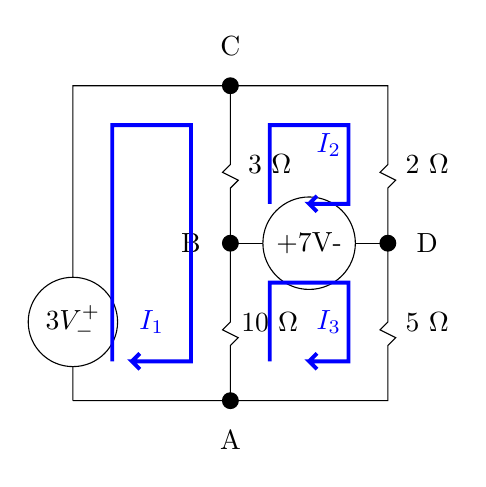
\begin{tikzpicture}
\draw (0,0)--(0,1)node[circle, draw=black, fill=white]{$3V_{-}^{+}$}--(0,4)--(2,4)--(2,3)
--(1.9,2.9)--(2.1,2.8)--(2,2.7)--(2,2)--(2,1)
--(1.9,.9)--(2.1,.8)--(2,.7)--(2,0)--(0,0);
\draw (2,4)--(4,4)--(4,3)
--(3.9,2.9)--(4.1,2.8)--(4,2.7)--(4,2);
\draw (2,2)--(3,2)node[circle, draw=black, fill=white]{+7V-}--(4,2);
\draw (4,2)--(4,1)
--(3.9,.9)--(4.1,.8)--(4,.7)--(4,0)--(2,0);
\draw node at (2.5,1) {10 $\Omega$};
\draw node at (4.5,1) {5 $\Omega$};
\draw node at (2.5,3) {3 $\Omega$};
\draw node at (4.5,3) {2 $\Omega$};
\draw node at (1.5,2) {B};
\draw node at (2,-.5) {A};
\draw node at (2,4.5) {C};
\draw node at (4.5,2) {D};
\filldraw (2,4) circle[radius=1 mm];
\filldraw (2,2) circle[radius=1 mm];
\filldraw (4,2) circle[radius=1 mm];
\filldraw (2,0) circle[radius=1 mm];
\draw [draw=blue, line width=0.5mm] (.5,.5)--(.5,3.5)--(1.5,3.5)
--(1.5,.5)--(.75,.5)--(.85,.4)--(.75,.5)--(.85,.6);
\draw [text=blue] node at (1,1) {$I_1$};
\draw [draw=blue, line width=0.5mm] (2.5,2.5)--(2.5,3.5)--(3.5,3.5)
--(3.5,2.5)--(3,2.5)--(3.1,2.4)--(3,2.5)--(3.1,2.6);
\draw [text=blue] node at (3.25,3.25) {$I_2$};
\draw [draw=blue, line width=0.5mm] (2.5,.5)--(2.5,1.5)--(3.5,1.5)
--(3.5,.5)--(3,.5)--(3.1,.4)--(3,.5)--(3.1,.6);
\draw [text=blue] node at (3.25,1) {$I_3$};
\end{tikzpicture}
\caption{Loops indicated in blue. Each loop has a current through it.}
\end{center}
\end{figure}

Note that the total current through the interior edges are combinations of these loop currents. For example, the current up through the $3 \Omega$ resistor is $I_2-I_1$.\par

Next, write KVL for each loop. There are two tricky parts to this.
\begin{itemize}
\item \textbf{First Tricky Thing:} Getting the signs right. More around each loop in clockwise direction. If you move from - to +, then add that voltage. If you move from + to - then subtract it. Recall that positive currents flow through resistors from + to -.
\item \textbf{Second Tricky Thing:} Handling components that have more than one loop current passing through it. The 3 Ohm resistor, for example, has $I_1$ passing through it from C to B and $I_2$ passing through it the other direction from B to C.
\end{itemize}

Write out KVL for each loop:
\begin{align*}
\text{First Loop (A-C-B-A):}&&+3-3(I_1-I_2)-10(I_1-I_3)&=0\\
\text{Second Loop (B-C-D-B):}&&-3(I_2-I_1)-2I_2+7V&=0\\
\text{Third Loop (A-B-D-A):}&&-10(I_3-I_1)-7V-5I_3&=0
\end{align*}

Put this in matrix form:
\begin{align}
\left[ \begin{matrix}
(-3-10)&	3&	10\\
3&	(-3-2)&0\\
10	&	0&	(-10-5)\\
\end{matrix} \right]
\left[ \begin{matrix}
I_1\\
I_2\\
I_3\\
\end{matrix} \right] =
\left[ \begin{matrix}
-3\\
-7\\
7\\
\end{matrix} \right]
\end{align}

\begin{blevel}
Determine the inverse of this matrix and write it down.
\end{blevel}

\begin{clevel}
Solve for the currents $I_1,I_2,I_3$.
\end{clevel}

\begin{clevel}
Suppose the direction of the 7V source were switched. Modify your equations and matrix and resolve for $I_1,I_2,I_3$.
\end{clevel}

\begin{dlevel}
Let's call the 7V source, $V_A$ and the 3V source, $V_B$. Why does the $V_A$ appear twice in on the right side of the equation while $V_B$ only appears once? Can $V_A$ appear three times? What assumptions have you made?
\end{dlevel}

\begin{dlevel}
What would happen to the algebra if we used all possible loops instead of just the loops that don't contain other loops?
\end{dlevel}

%%%%%%%%%%%%%%%%%%%%%%%%%%%%%%%%%%%%%%%%%%%%%%%%%
\subsection{Loop Analysis with Current Sources}
In this section, we will replace the 7V source with a 3A current source. This causes just a little trouble because we no longer know the voltage from B to D. No worries - just assign it a variable, like $V_1$ \footnote{Do you see the similarity to nodal analysis?}. 
\par
But, we now have one too many unknowns. We need another equation. Solution: We can use information about what the current source is doing. The current source is forcing the current from B to D to be 3A. That current from B to D is $I_3-I_2$, so we can write $I_3-I_2=3 A$.

\begin{figure}[H]
\begin{center}
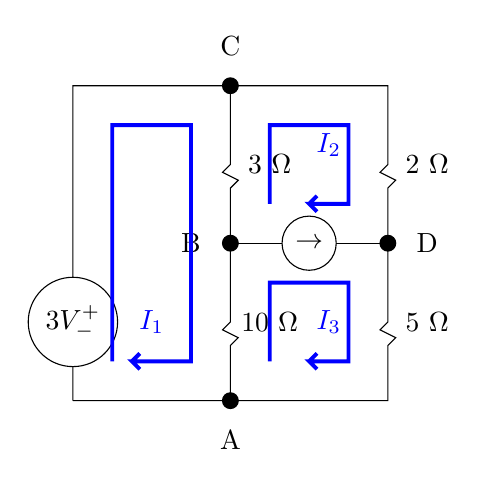
\begin{tikzpicture}
\draw (0,0)--(0,1)node[circle, draw=black, fill=white]{$3V_{-}^{+}$}--(0,4)--(2,4)--(2,3)
--(1.9,2.9)--(2.1,2.8)--(2,2.7)--(2,2)--(2,1)
--(1.9,.9)--(2.1,.8)--(2,.7)--(2,0)--(0,0);
\draw (2,4)--(4,4)--(4,3)
--(3.9,2.9)--(4.1,2.8)--(4,2.7)--(4,2);
\draw (2,2)--(3,2)node[circle, draw=black, fill=white]{$\rightarrow$}--(4,2);
\draw (4,2)--(4,1)
--(3.9,.9)--(4.1,.8)--(4,.7)--(4,0)--(2,0);
\draw node at (2.5,1) {10 $\Omega$};
\draw node at (4.5,1) {5 $\Omega$};
\draw node at (2.5,3) {3 $\Omega$};
\draw node at (4.5,3) {2 $\Omega$};
\draw node at (1.5,2) {B};
\draw node at (2,-.5) {A};
\draw node at (2,4.5) {C};
\draw node at (4.5,2) {D};
\filldraw (2,4) circle[radius=1 mm];
\filldraw (2,2) circle[radius=1 mm];
\filldraw (4,2) circle[radius=1 mm];
\filldraw (2,0) circle[radius=1 mm];
\draw [draw=blue, line width=0.5mm] (.5,.5)--(.5,3.5)--(1.5,3.5)
--(1.5,.5)--(.75,.5)--(.85,.4)--(.75,.5)--(.85,.6);
\draw [text=blue] node at (1,1) {$I_1$};
\draw [draw=blue, line width=0.5mm] (2.5,2.5)--(2.5,3.5)--(3.5,3.5)
--(3.5,2.5)--(3,2.5)--(3.1,2.4)--(3,2.5)--(3.1,2.6);
\draw [text=blue] node at (3.25,3.25) {$I_2$};
\draw [draw=blue, line width=0.5mm] (2.5,.5)--(2.5,1.5)--(3.5,1.5)
--(3.5,.5)--(3,.5)--(3.1,.4)--(3,.5)--(3.1,.6);
\draw [text=blue] node at (3.25,1) {$I_3$};
\end{tikzpicture}
\caption{Loop analysis with a current source}
\end{center}
\end{figure}

\begin{clevel}
Write down the modified set of equations with the current source described above. Put it in matrix form. Solve for $I_1,I_2,I_3, V_1$.
\end{clevel}

\begin{clevel}
A circuit has more voltage sources than current sources. Knowing nothing else, do you think it would be easier to use loop analysis or nodal analysis? 
\end{clevel}


\begin{clevel}
A circuit has the structure shown in figure. It contains 2 voltage sources and 1 current source. How many equations will be produced by the loop analysis method? 

\begin{figure}[H]
\begin{center}
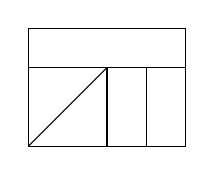
\begin{tikzpicture}
\draw (0,0)--(0,1.5)--(2,1.5)--(2,0)--(0,0);
\draw (0,1)--(2,1) (1,1)--(1,0);
\draw (0,0)--(1,1);
\draw (1.5,1)--(1.5,0);
\end{tikzpicture}
\caption{Circuit structure.}
\label{F:4RECT2}
\end{center}
\end{figure}

\end{clevel}
%%%%%%%%%%%%%%%%%%%%%%%%%%%%%%%%%%%%%%%%%%%%%%%%%%%%%%%%%%
\section{Source Transformations}
Earlier in this book, we simplified circuits by combining series or parallel connections of resistors. In this section, we'll get even more serious about simplication. We'll see that we can transform voltage sources into equivalent current sources and visa versa. By transforming sources at our convenience we can then combine parallel sets of current sources or series combinations of voltage sources.\par
First, though, we need to broaden our model of a voltage source.

\subsection{Improved model of a Voltage Source}
Consider an ideal voltage source connected to a resistor as shown in Figure~\ref{F:4RVA}:

\begin{figure}[H]
\begin{center}
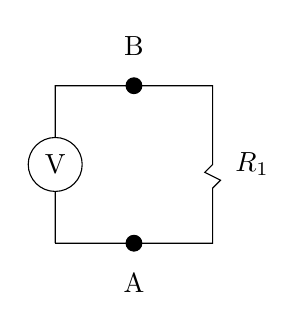
\begin{tikzpicture}
\draw (0,0)--(0,1)node[circle, draw=black, fill=white]{V}--(0,2)--(2,2)
--(2,1)--(1.9,.9)--(2.1,.8)--(2,.7)--(2,0)--(0,0);
\draw node at (2.5,1) {$R_1$};
\draw node at (1,2.5) {B};
\draw node at (1,-.5) {A};
\filldraw (1,2) circle[radius=1 mm];
\filldraw (1,0) circle[radius=1 mm];
\end{tikzpicture}
\caption{Ideal voltage source connected to a resistive load.}
\label{F:4RVA}
\end{center}
\end{figure}

The current through $R_1$ would be $\frac{V}{R_1}$. If $R_1$ were small, this current would get very big. If $R_1$ were infinitely small, the current would get infinitely big. \par
But this can't happen - there aren't any voltage sources that can deliver infinitely large current. Currents cause magnetic fields. An infinite current would cause an infinitely large magnetic field. If that doesn't impress you, the power consumed would also be infinite.

\begin{blevel}
What would be the magnetic field a distance of 3 cm away from a wire carrying 5A of current?
\end{blevel}

\begin{clevel}
For the circuit shown in Figure~\ref{F:4RVA}, with voltage V and resistance $R_1$, determine the power absorbed by the resistor as a function of V and $R_1$ only. What happens to the power absorbed in the $\lim_{R_1 \to 0}$? 
\end{clevel}

To make a better model \footnote{I say \emph{``better model"} because these are all approximate models, some better than others.} of a voltage source, we might add a resistor in series with the ideal voltage source. Maybe this resistance models some metal inside the box, or maybe a contact at the edge, but it also models any effect that tends to limit the amount of current that the source can produce.
\par
Our new model looks like Figure~\ref{F:4RVB}.

\begin{figure}[H]
\begin{center}
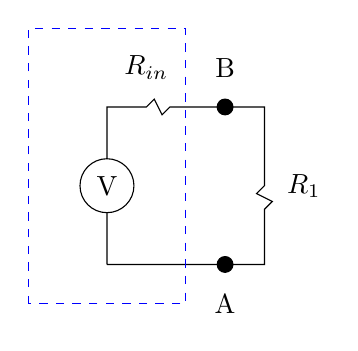
\begin{tikzpicture}
\draw (0,0)--(0,1)node[circle, draw=black, fill=white]{V}--(0,2)
--(.5,2)--(.6,2.1)--(.7,1.9)--(.8,2)
--(2,2)--(2,1)--(1.9,.9)--(2.1,.8)--(2,.7)--(2,0)--(0,0);
\draw node at (2.5,1) {$R_1$};
\draw node at (0.5,2.5) {$R_{in}$};
\draw node at (1.5,2.5) {B};
\draw node at (1.5,-.5) {A};
\draw [dashed, draw=blue] (-1,-.5)--(-1,3)--(1,3)--(1,-.5)--(-1,-.5);
\filldraw (1.5,2) circle[radius=1 mm];
\filldraw (1.5,0) circle[radius=1 mm];
\end{tikzpicture}
\caption{Real voltage source connected to a resistive load. The blue dashed box indicates the voltage source.}
\label{F:4RVB}
\end{center}
\end{figure}

\begin{blevel}
What is the current through $R_1$ in the $\lim_{R_1 \to 0}$? 
\end{blevel}

\begin{blevel}
Suppose $R_1$ were 50 $\Omega$. What would be the voltage across $R_1$ if the voltage source were a 9V battery with 7 $\Omega$ of internal resistance?  
\end{blevel}

\begin{blevel}
What is the voltage across $R_1$ in terms of V, $R_1$ and $R_{in}$? 
\end{blevel}

\begin{clevel}
Find the power absorbed by $R_1$ as a function of $R_{in}$ and V. What value of $R_1$, in terms of $R_{in}$, will result in the maximum amount of power absorbed by $R_1$? Hint: can you use calculus to determine the maximum of a function?
\end{clevel}

%%%%%%%%%%%%%%%%%%%%%%%%%%%%%%%%%
\subsection{Equivalent Sources}
Suppose we have a mysterious box - maybe someone claims its a voltage source, maybe not. We make some measurements to try to learn about what's inside the box. 

\begin{figure}[H]
\begin{center}
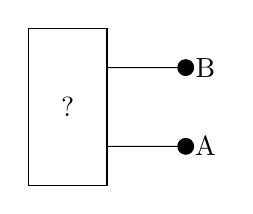
\begin{tikzpicture}
\draw (0,0) rectangle node{?} (1,2);
\draw node at (2.25,1.5) {B};
\draw node at (2.25,.5) {A};
\filldraw (1,1.5)--(2,1.5) circle[radius=1 mm];
\filldraw (1,.5)--(2,.5) circle[radius=1 mm];
\end{tikzpicture}
\caption{Mysterious box}
\end{center}
\end{figure}

First, we measure the voltage from A to B. We get 5V. Then we connect an ammeter between B and A and get 1A. We conclude that the black box could be the following:
\par
\begin{figure}[H]
\begin{center}
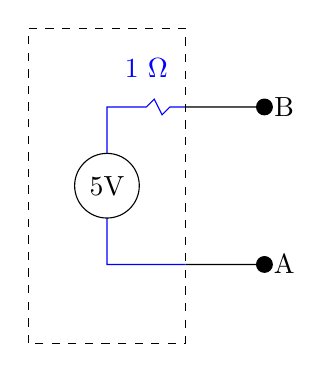
\begin{tikzpicture}
\draw [draw=blue] (1,0)--(0,0)--(0,1)node[circle, draw=black, fill=white]{5V}--(0,2)
--(.5,2)--(.6,2.1)--(.7,1.9)--(.8,2)--(1,2);
\draw node[text=blue] at (0.5,2.5) {1 $\Omega$};
\draw [dashed] (-1,-1) rectangle node{} (1,3);
\draw node at (2.25,2) {B};
\draw node at (2.25,0) {A};
\filldraw (1,2)--(2,2) circle[radius=1 mm];
\filldraw (1,0)--(2,0) circle[radius=1 mm];
\end{tikzpicture}
\caption{Mysterious box guess.}
\label{F:4TH}
\end{center}
\end{figure}

Ammeters act like a shorts, so the measured current would be 1A. Voltmeters act like open circuits, so there would be no current through the internal 1 $\Omega$ resistor and therefore no voltage drop across it. The voltmeter would read 5V.

\begin{figure}[H]
\begin{center}
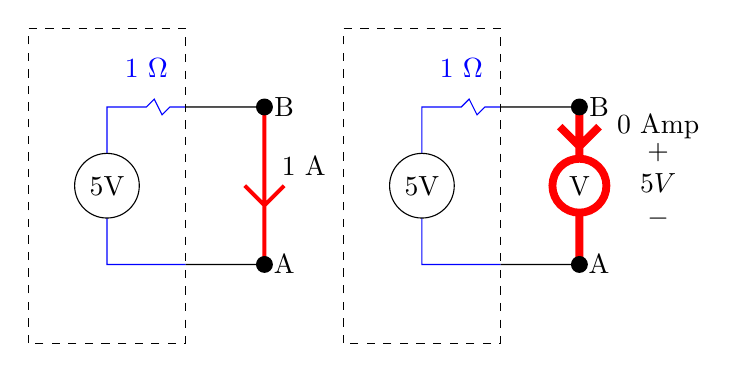
\begin{tikzpicture}
\draw [draw=blue] (1,0)--(0,0)--(0,1)node[circle, draw=black, fill=white]{5V}--(0,2)
--(.5,2)--(.6,2.1)--(.7,1.9)--(.8,2)--(1,2);
\draw node[text=blue] at (0.5,2.5) {1 $\Omega$};
\draw [dashed] (-1,-1) rectangle node{} (1,3);
\draw node at (2.25,2) {B};
\draw node at (2.25,0) {A};
\draw [draw=red, line width=0.5mm](2,2)--(2,0) (1.75,1)--(2,0.75)--(2.25,1);
\draw node at (2.5,1.25) {1 A};
\filldraw (1,2)--(2,2) circle[radius=1 mm];
\filldraw (1,0)--(2,0) circle[radius=1 mm];

\draw [draw=blue] (5,0)--(4,0)--(4,1)node[circle, draw=black, fill=white]{5V}--(4,2)
--(4.5,2)--(4.6,2.1)--(4.7,1.9)--(4.8,2)--(5,2);
\draw node[text=blue] at (4.5,2.5) {1 $\Omega$};
\draw [dashed] (3,-1) rectangle node{} (5,3);
\draw node at (6.25,2) {B};
\draw node at (6.25,0) {A};
\draw [draw=red, line width=1mm](6,2)--(6,1)node[circle, draw=red, fill=white]{V}--(6,0) (5.75,1.75)--(6,1.5)--(6.25,1.75);
\draw node at (7,1.75) {0 Amp};
\filldraw (5,2)--(6,2) circle[radius=1 mm];
\filldraw (5,0)--(6,0) circle[radius=1 mm];
\draw node at (7,1){$\begin{matrix}+\\5V\\-\end{matrix}$};
\end{tikzpicture}
\caption{Current measurement (left) and voltage measurement (right).}
\label{F:4TH2}
\end{center}
\end{figure}
\par
But the circuit in Figure~\ref{F:NotSpecial} would also work, an ammeter connected from B to A would read 1A and a voltmeter would read 5V.
\par
\begin{figure}[H]
\begin{center}
\begin{tikzpicture}
\draw [draw=blue] (1,0)--(-1,0)--(-1,1)node[circle, draw=black, fill=white]{10V}--(-1,2)--(0,2)--(0,1.5)--(-.1,1.4)--(.1,1.3)--(0,1.2)--(0,1);
\draw [draw=blue] (0,1)--(0,.5)--(-.1,.4)--(.1,.3)--(0,.2)--(0,0)--(-1,0);
\draw node[text=blue] at (.5,1.5) {2 $\Omega$};
\draw node[text=blue] at (.5,0.5) {2 $\Omega$};
\draw [dashed] (-2,-1) rectangle node{} (1,3);
\draw node at (2.25,1) {B};
\draw node at (2.25,0) {A};
\filldraw [draw=blue] (0,1) circle[radius=1 mm]--(1,1);
\filldraw (1,1)--(2,1) circle[radius=1 mm];
\filldraw (1,0)--(2,0) circle[radius=1 mm];
\end{tikzpicture}
\caption{A second option for the contents of the mysterious Box.}
\label{F:NotSpecial}
\end{center}
\end{figure}

Now here comes a surprising claim:\\
\\
\noindent
\textbf{Claim:} These two mystery implementations (Figure~\ref{F:NotSpecial} and Figure~\ref{F:4TH}) will produce the same voltages and currents no matter what combination of resistors, voltages, current sources, and multimeters connect to A and B \footnote{Outside the box. Inside the box, things will be different.}. This is a version of what is often credited as \textbf{Thev\'enin's Theorem}.

\begin{alevel}
If a resistor, R, were connect from B to A on the outside of the box for for Figure~\ref{F:4TH}, what would be the current through that resistor (in terms of R)?
\end{alevel}

\begin{clevel}
Suppose a resistor, R, were connected from B to A on the outside of the box for Figure~\ref{F:NotSpecial} what would be the current through that resistor (in terms of R)?
\end{clevel}

Figure~\ref{F:4NOR} shows another version for our black box. Let's find values so that it also behaves like the other circuits.

\begin{figure}[H]
\begin{center}
\begin{tikzpicture}
\draw [draw=blue] (1,0)--(-1,0)--(-1,1)node[circle, draw=blue, fill=white]{$\uparrow$}--(-1,2)--(0,2)--(0,1.5)--(-.1,1.4)--(.1,1.3)--(0,1.2)--(0,1);
\draw [draw=blue] (0,1)--(0,0)--(-1,0);
\draw node[text=blue] at (.5,1.5) {R};
\draw node[text=blue] at (-.5,1) {I};
\draw [dashed] (-2,-1) rectangle node{} (1,3);
\draw node at (2.25,2) {B};
\draw node at (2.25,0) {A};
\filldraw [draw=blue] (0,0) circle[radius=1 mm];
\filldraw [draw=blue] (0,2) circle[radius=1 mm]--(1,2);
\filldraw (1,2)--(2,2) circle[radius=1 mm];
\filldraw (1,0)--(2,0) circle[radius=1 mm];
\end{tikzpicture}
\caption{Circuit Z. Norton Equivalent. Current Source Version}
\label{F:4NOR}
\end{center}
\end{figure}

\begin{table}[H]
\begin{center}
\begin{tabular}{|c|c|p{60mm}|} \hline
Requirement & Conclusion & Reasoning \\ \hline
Voltmeter reads 5V & IR=5V & The volt-meter measures the voltage across the resistor. \\ \hline
Ammeter reads 1A & I=1A	& Since ammeters have little resistance, all the current will flow through the ammeter. Therefore, the current source must be 1A. \\ \hline
\end{tabular}
\end{center}
\end{table}

Finally, since I=1A and IR=5V, then the resistance R must be 5 $\Omega$. According to Thevenin's Theorem, this version is now electrically indistinguishable from the other versions.
\\

We will refer to the voltage source-resistor series combination shown in Figure~\ref{F:4TH} as the Th\'{e}venin equivalent, and refer to the parallel current source-resistor combination as the Norton equivalent. 
\par
To spare some writing, this book introduces a short-hard for these versions. A source, whether Th\'{e}venin or Norton, requires two numbers. We will put them in paranthesis with a comma between the source and the resistance\footnote{Why not write them as a matrix? Answer: They don't add like matrices would and writing them that way might make that tempting.}. The unit and the subscript redundantly identify it as a voltage or avcurrent source. For example, we would capture Figure~\ref{F:4NOR} as: $Z_N=(1A,5\Omega)$. It's Th\'{e}venin version would be $Z_T=(5V,5\Omega)$.
\par
\begin{alevel}
Sketch both versions of the circuit described as $W_V=(12V,5\Omega)$. 
\end{alevel}

\begin{blevel}
Fill in the following table regarding some circuit W:
\begin{table}[H]
\begin{center}
\begin{tabular}{|c|c|} \hline
Th\'{e}venin version & Norton Version \\ \hline
&$W_N=(3A,10\Omega)$ \\ \hline
$W_V=(3V,10\Omega)$& \\ \hline
$W_V=(12V,5\Omega)$& \\ \hline
\end{tabular}
\end{center}
\end{table}
\end{blevel}


But when should we prefer one version over another?
\begin{itemize}
\item If two sources are in series, the voltage equivalents will probably be easier to combine.
\item If two sources are in parallel, the current source versions will probably be easier to combine.
\end{itemize}

It might help to reorder the drawing of parallel components to make it easier to see that the resistors are in parallel and that the two parallel current sources both push current into the same node and therefore add with each other. Figure~\ref{F:4STCOM} shows this. \\

\begin{figure}[H]
\begin{center}
\begin{tikzpicture}
\draw (0,0)--(0,1)node[circle, draw=black, fill=white]{$\uparrow$}
--(0,2)--(1,2)--(1,1)--(1.1,.9)--(.9,.8)--(1,.7)--(1,0)--(0,0);
\draw (2,0)--(2,1)node[circle, draw=black, fill=white]{$\uparrow$}
--(2,2)--(3,2)--(3,1)--(3.1,.9)--(2.9,.8)--(3,.7)--(3,0)--(2,0);
\draw (2,0)--(1,0) (2,2)--(1,2);
\filldraw (1.5,0) circle[radius=1 mm];
\filldraw (1.5,2) circle[radius=1 mm];
\draw (6,0)--(6,1)node[circle, draw=black, fill=white]{$\uparrow$}--(6,2);
\draw (8,2)--(8,2)--(8,1)--(8.1,.9)--(7.9,.8)--(8,.7)--(8,0)--(8,0);
\draw (7,0)--(7,1)node[circle, draw=black, fill=white]{$\uparrow$}--(7,2);
\draw (9,2)--(9,2)--(9,1)--(9.1,.9)--(8.9,.8)--(9,.7)--(9,0)--(9,0);
\draw (9,0)--(6,0) (9,2)--(6,2);
\filldraw (7.5,0) circle[radius=1 mm];
\filldraw (7.5,2) circle[radius=1 mm];
\draw node at (4.5,1) {$\rightarrow$};
\end{tikzpicture}
\caption{Redrawing Parallel Norton Equivalents to make clear parallel combinations.}
\label{F:4STCOM}
\end{center}
\end{figure}

As we analyze circuits, we will look for situations when it is advantageous transform from Thevenin to Norton or visa versa.

\begin{blevel}
Consider two circuits, W and Y, that are in series. $W_T=(3V,10\Omega)$ and $Y_T=(-2V,2\Omega)$. Combine them and report the combined Thevenin equivalent. Draw the new circuit.
\end{blevel}

\begin{clevel}
Consider two circuits, W and Y, that are in series. $W_N=(3A,10\Omega)$ and $Y_T=(-2V,2\Omega)$. Combine them and report the combined Thevenin equivalent. Draw the new circuit.
\end{clevel}

%%%%%%%%%%%%%%%%%%%%%%%%%%%%%%%%%%%%%%%%%%%%
\subsection{Source Transformation Example}
Let's find the current through the 2 Ohm resistor for the circuit shown in Figure~\ref{F:4STEX}. Look at the circuit diagram and try to identify some Th\'{e}venin and Norton sources.

\begin{figure}[H]
\begin{center}
\begin{tikzpicture}
\draw (0,0)--(-1,0)--(-1,1)--(-1.1,1.1)--(-.9,1.2)--(-1,1.3)--(-1,4)--(0,4);
\draw (1,0)--(0,0)--(0,1) node[circle, draw=black, fill=white]{$\uparrow$}--(0,4)--(1,4);
\draw (1,0)--(1,1) node[circle, draw=black, fill=white]{5V}--
(1,2)--(1.1,2.1)--(.9,2.2)--(1,2.3)--(1,4);
\filldraw (1,0) circle[radius=1 mm];
\filldraw (1,4) circle[radius=1 mm];
\filldraw (4,4) circle[radius=1 mm];
\filldraw (0,4) circle[radius=1 mm];
\filldraw (0,0) circle[radius=1 mm];
\filldraw (4,0) circle[radius=1 mm];
\draw node at (-.5,1.5) {3 A};
\draw node at (-1.5,1) {5 $\Omega$};
\draw node at (1.5,2.25) {7 $\Omega$};
\draw node at (2,4.5) {3 $\Omega$};
\draw node at (6.5,2.5) {2 $\Omega$};
\draw node at (4.5,2.5) {10 $\Omega$};
\draw (1,4)--(2,4)--(2.1,4.1)--(2.2,3.9)--(2.3,4)--(3,4)node[circle, draw=black,fill=white]{7V}--(4,4);
\draw node at (3.4,3.5){+};
\draw node at (2.6,3.5){-};
\draw (4,4)--(4,3)--(4.1,2.9)--(3.9,2.8)--(4.1,2.7)--(4,2.6)--(4,0)--(1,0);
\draw (4,4)--(6,4)--(6,3)--(6.1,2.9)--(5.9,2.8)--(6,2.7)--(6,0)--(4,0);
\end{tikzpicture}
\caption{Source transformation example. Unsimplified circuit.}
\label{F:4STEX}
\end{center}
\end{figure}

Figure~\ref{F:4STEXID} identifies some Thevenin and Norton combinations and labels them A,B,C and D. Maybe the most surprising is D. While just a resistor, it's equivalent to a resistor in series with a 0V source\footnote{Or in parallel with a 0 Amp current source.}.

\begin{figure}[H]
\begin{center}
\begin{tikzpicture}
\draw (0,0)--(-1,0)--(-1,1)--(-1.1,1.1)--(-.9,1.2)--(-1,1.3)--(-1,4)--(0,4);
\draw (1,0)--(0,0)--(0,1) node[circle, draw=black, fill=white]{$\uparrow$}--(0,4)--(1,4);
\draw (1,0)--(1,1) node[circle, draw=black, fill=white]{5V}--
(1,2)--(1.1,2.1)--(.9,2.2)--(1,2.3)--(1,4);
\filldraw (1,0) circle[radius=1 mm];
\filldraw (1,4) circle[radius=1 mm];
\filldraw (4,4) circle[radius=1 mm];
\filldraw (0,4) circle[radius=1 mm];
\filldraw (0,0) circle[radius=1 mm];
\filldraw (4,0) circle[radius=1 mm];
\draw node at (-.5,1.5) {3 A};
\draw node at (-1.5,1) {5 $\Omega$};
\draw node at (1.5,2.25) {7 $\Omega$};
\draw node at (2,4.5) {3 $\Omega$};
\draw node at (6.5,2.5) {2 $\Omega$};
\draw node at (4.5,2.5) {10 $\Omega$};
\draw (1,4)--(2,4)--(2.1,4.1)--(2.2,3.9)--(2.3,4)--(3,4)node[circle, draw=black,fill=white]{7V}--(4,4);
\draw (4,4)--(4,3)--(4.1,2.9)--(3.9,2.8)--(4.1,2.7)--(4,2.6)--(4,0)--(1,0);
\draw (4,4)--(6,4)--(6,3)--(6.1,2.9)--(5.9,2.8)--(6,2.7)--(6,0)--(4,0);
\draw [dashed, draw=blue] (2.5,4) ellipse (1.25 cm and 1 cm);
\draw [dashed, draw=blue] (-1,1) ellipse (1.25 cm and 1 cm);
\draw [dashed, draw=blue] (1,1) ellipse (.5 cm and 1.75 cm);
\draw [dashed, draw=blue] (4,2) ellipse (.5 cm and 1.75 cm);
\draw node[text=blue] at (-2,2) {A};
\draw node[text=blue] at (2.,2) {B};
\draw node[text=blue] at (3,5.25) {C};
\draw node[text=blue] at (5,2) {D};
\end{tikzpicture}
\caption{Source transformation example with strategy identified.}
\label{F:4STEXID}
\end{center}
\end{figure}

Sources A and B are in parallel. That combination is in series with source C. That total combination is in parallel with source D. That whole mess is then both in series and/or parallel with the 2 Ohm resistor. We can distill all that into this expression:\\

\begin{align}
\text{circuit (excluding 2 Ohm)} =((A \parallel B)+C) \parallel D)
\end{align}

Now let's work out the details:

\begin{enumerate}
\item To combine A and B in parallel, they should both be Norton equivalents. $A_N=(3A,5\Omega)$ and $B_N=(\frac{5}{7}A,7\Omega)$. Combined $(A\parallel B)_N=(3\frac{5}{7}A,\frac{35}{12}\Omega)$.
\item To combine $(A \parallel B)$ in series with C, it should both be written as a  Thevenin equivalent: $(A \parallel B)_T = (10.83V, \frac{35}{12}\Omega)$ and $C_T=(7V,3\Omega)$. This gives $(A \parallel B)_T+C_T = (17.83V,5.92\Omega)$.
\item To combine this in parallel with D, go back to the Norton version. $((A \parallel B)+C)_N = (3.014A,5.92\Omega)$, and $D_N=(0A, 10\Omega)$. Combined gives, $((A \parallel B)+C)\parallel D)_N=(3.014A,3.72\Omega)$.
\item Taking this back to Th\'{e}venin format: $((A \parallel B)+C)\parallel D)_T=(11.2V,3.72\Omega)$.
\item Now the circuit looks like Figure~\ref{F:Simplified} and the current through the $2 \Omega$ resistor can be calculated to be $\frac{11.2V}{5.72\Omega} = 1.97 A$. Done.
\end{enumerate}

\begin{figure}[H]
\begin{center}
\begin{tikzpicture}
\draw (0,0)--(0,2) node[circle, draw=black, fill=white]{$\begin{matrix}+\\11.2V\\-\end{matrix}$}--(0,4)--(1,4)
--(1.1,4.1)--(1.2,3.9)--(1.3,4)--(2,4)
--(2,3)--(1.9,2.9)--(2.1,2.8)--(2,2.7)--(2,0)--(0,0);;
\draw node at (1.5,2.25) {2 $\Omega$};
\draw node at (1.5,4.5) {3.72 $\Omega$};
\end{tikzpicture}
\caption{Simplied Circuit after Source Transformations}
\label{F:Simplified}
\end{center}
\end{figure}

\begin{clevel}
Reconsider Figure~\ref{F:4STEX}. This time use the procedure to the determine the current through the 5 Ohm resistor. Start at the right side of the diagram and work your way to the left. Hint: Start by combining the 10 and 2 Ohm resistors in parallel and then in series with combo C.
\end{clevel}

%%%%%%%%%%%%%%%%%%%%%%%%%%%%%%%%%%%%%%%%%%%%%%%%%%%%%%%%%%
\section{Superposition and Linearity}
\textbf{A Superposition Situation:} Imagine you work at a coffee shop. While you work, the shop sells \$60 of coffee per hour. A different employee, J, working a different shift, sells \$50 of coffee per hour. The shop considers having you both work at the same time. Do you suppose the shop will sell \$110 of coffee?\\
\\
If the coffee shop behaves as a \textbf{linear system}, then together you would earn \$110. The contributions of you and J can be added (superimposed) together.
\par
Let's capture this idea with an equation (`I' represents the coffee shop's income):

\begin{align*}
I(you+J) = I(you)+I(J)
\end{align*}

Or more generally\footnote{For linear systems, the claim is often written as: $f(\alpha x,\beta y) = \alpha f(x)+\beta f(y)$.},

\begin{align}
f(x+y) = f(x)+f(y) \label{E:4LIN}
\end{align}

Note that for a linear system it would follow that, 
\begin{align*}
f(x+x) &= f(x)+f(x) \\
f(2x)&=2f(x)
\end{align*}
Maybe you can convince yourself that $f(kx)=kf(x)$.\par

\begin{alevel}
How much income would the coffee shop make per hour if two clones of you were to work at the same time? Assume superposition holds.
\end{alevel}

\begin{bigidea} Many engineering systems can be approximated as linear systems.
\end{bigidea}

Equation~\eqref{E:4LIN} does not usually exactly apply\footnote{Remember, Ohm's Law is just an approximation.}, but in many cases, linearity applies closely enough that\footnote{Sometimes not even that closely!} the mathematical benefit makes the linearity assumption worthwhile.
\par
\textbf{Claim:} If a circuit contains only voltage/current sources and resistors, then the circuit will behave as a linear system. \par
Imagine a circuit with three sources and one output voltage of interest, $V_{out}$. $V_{out}$ would be some function of the three sources, $S_1,S_2,S_3$.
\par
\begin{align}
V_{out} = f(S_1,S_2,S_3)
\end{align}

If the system is linear, then:
\par
\begin{align}
V_out &= f(S_1,S_2,S_3) \notag\\
	&= f(S_1,0,0)+f(0,S_2,0)+f(0,0,S_3) \label{E:4LIN2}
\end{align}

The zeros indicate that source has been turned off (0V for a voltage source, or 0 Amps for a current source). This would also be true, but probably not as useful:
\par
\begin{align}
V_out &= f(S_1,S_2,S_3) \\
	&= f(S_1,4S_2,.5S_3)+f(0,-3S_2,0)+f(0,0,0.5S_3)
\end{align}

We plan to determine $V_{out}$ by summing together the individual contributions due to each source, with the other sources turned off. In other words, we'll use Equation~\eqref{E:4LIN2}. To turn off a power source:\

\begin{itemize}
\item If it's a voltage source, set the voltage to zero by replacing it with the short circuit (an open circuit could still have a voltage difference across it).
\item If it's a current source, make the current through it zero by replacing it with an open circuit (a short circuit could still have current through it)
\end{itemize}

\begin{blevel}
A linear circuit has two sources, a 5A current source and a 3V voltage source. The output due to just the 5A current source is 3.5V and the output due to just the 3V source is 17 Volts. What will the output be with both sources on at the same time?
\end{blevel}

\begin{clevel}
A linear circuit has two sources, a 5A current source and a 3V voltage source. The output due to just the 5A current source is 3.5V and the output due to just the 3V source is 17 Volts. What will the output be with the current source set to 10A and the voltage source set to 9V?
\end{clevel}

\begin{alevel}
For the coffee shop, what would be:
\begin{align*}
I(0.5*you,3*Friend)=?\\
I(0,3*Friend)+I(0.5*you,0)=?
\end{align*}
\end{alevel}

%%%%%%%%%%%%%%%%%%%%%%%%%%%%%%%%%%
\subsection{Superposition Example}
Let's try an example like the Figure~\ref{F:4NODV}. The output voltage ($V_{out}$) will be the voltage drop across the 5 $\Omega$ resistor ($V_{DA}$).

\begin{figure}[H]
\begin{center}
\begin{tikzpicture}
\draw (0,0)--(0,1)node[circle, draw=black, fill=white]{$\uparrow$}--(0,4)--(2,4)--(2,3)
--(1.9,2.9)--(2.1,2.8)--(2,2.7)--(2,2)--(2,1)
--(1.9,.9)--(2.1,.8)--(2,.7)--(2,0)--(0,0);
\draw (2,4)--(4,4)--(4,3)
--(3.9,2.9)--(4.1,2.8)--(4,2.7)--(4,2);
\draw (2,2)--(3,2)node[circle, draw=black, fill=white]{+7V-}--(4,2);
\draw (4,2)--(4,1)
--(3.9,.9)--(4.1,.8)--(4,.7)--(4,0)--(2,0);
\draw node at (-1,1) {3 A};
\draw node at (2.5,1) {10 $\Omega$};
\draw node at (4.5,1) {5 $\Omega$};
\draw node at (2.5,3) {3 $\Omega$};
\draw node at (4.5,3) {2 $\Omega$};
\draw node at (1.5,2) {B};
\draw node at (2,-.5) {A};
\draw node at (2,4.5) {C};
\draw node at (4.5,2) {D};
\filldraw (2,4) circle[radius=1 mm];
\filldraw (2,2) circle[radius=1 mm];
\filldraw (4,2) circle[radius=1 mm];
\filldraw (2,0) circle[radius=1 mm];
\end{tikzpicture}
\caption{Superposition example}
\end{center}
\end{figure}

The principle of superposition says that $V_{out}$ depends on the 3A current source (with the 7V source shorted) and the 7V source with the 3A current source as an open circuit. We'll structure our answer so that we don't lose track:

\begin{align*}
V_{out}(3A, 7V)&=V_{out}(3A,0)+V_{out}(0, 7V)\\
V_{out}&=\underbrace{\rule{1 cm}{.25 mm}}_{3A}+\underbrace{\rule{1 cm}{.25 mm}}_{7V}
\end{align*}

First, with the 7V source shorted:

\begin{figure}[H]
\begin{center}
\begin{tikzpicture}
\draw (0,0)--(0,1)node[circle, draw=black, fill=white]{$\uparrow$}--(0,4)--(2,4)--(2,3)
--(1.9,2.9)--(2.1,2.8)--(2,2.7)--(2,2)--(2,1)
--(1.9,.9)--(2.1,.8)--(2,.7)--(2,0)--(0,0);
\draw (2,4)--(4,4)--(4,3)
--(3.9,2.9)--(4.1,2.8)--(4,2.7)--(4,2);
\draw (2,2)--(3,2)--(4,2);
\draw (4,2)--(4,1)
--(3.9,.9)--(4.1,.8)--(4,.7)--(4,0)--(2,0);
\draw node at (-1,1) {3 A};
\draw node at (2.5,1) {10 $\Omega$};
\draw node at (4.5,1) {5 $\Omega$};
\draw node at (2.5,3) {3 $\Omega$};
\draw node at (4.5,3) {2 $\Omega$};
\draw node at (1.5,2) {B};
\draw node at (2,-.5) {A};
\draw node at (2,4.5) {C};
%\draw node at (4.5,2) {D};
\filldraw (2,4) circle[radius=1 mm];
\filldraw (2,2) circle[radius=1 mm];
\filldraw (4,2) circle[radius=1 mm];
\filldraw (2,0) circle[radius=1 mm];
\end{tikzpicture}
\caption{Superposition example with 7V source (turned off) shorted.}
\end{center}
\end{figure}

Solving for $V_{out}$ still takes several steps:

\begin{enumerate}
\item Observe that B and D are now the same node (they are connected by a perfect wire).
\item Observe that the 3 and 2 Ohm resistors are in parallel, as are the 10 and 5 Ohm resistors.
\item Combine the two parallel combinations to get:
\begin{align*}
R_{CB}=3\parallel 2=1.2 \Omega && R_{BA}=10\parallel 5=3.33 \Omega
\end{align*}

\item The current source forces 3A through both the 1.2 and 3.33 $\Omega$ resistors. A voltage drop $V_{BA}$ results: $V_{BA}=IR=3*3.33 = 10V$.
\end{enumerate}

Then, with the 7V source turned back on and the 3A current source set to zero (disconnected):

\begin{figure}[H]
\begin{center}
\begin{tikzpicture}
\draw (0,0)--(0,1) (0,3)--(0,4)--(2,4)--(2,3)
--(1.9,2.9)--(2.1,2.8)--(2,2.7)--(2,2)--(2,1)
--(1.9,.9)--(2.1,.8)--(2,.7)--(2,0)--(0,0);
\draw (2,4)--(4,4)--(4,3)
--(3.9,2.9)--(4.1,2.8)--(4,2.7)--(4,2);
\draw (2,2)--(3,2)node[circle, draw=black, fill=white]{+7V-}--(4,2);
\draw (4,2)--(4,1)
--(3.9,.9)--(4.1,.8)--(4,.7)--(4,0)--(2,0);
%\draw node at (-1,1) {3 A};
\draw node at (2.5,1) {10 $\Omega$};
\draw node at (4.5,1) {5 $\Omega$};
\draw node at (2.5,3) {3 $\Omega$};
\draw node at (4.5,3) {2 $\Omega$};
\draw node at (1.5,2) {B};
\draw node at (2,-.5) {A};
\draw node at (2,4.5) {C};
\draw node at (4.5,2) {D};
\filldraw (2,4) circle[radius=1 mm];
\filldraw (2,2) circle[radius=1 mm];
\filldraw (4,2) circle[radius=1 mm];
\filldraw (2,0) circle[radius=1 mm];
\end{tikzpicture}
\caption{Superposition example with 3A source turned off (open circuit)}
\end{center}
\end{figure}

Observe that the 5 and 10 $\Omega$ resistors are now in series. By voltage division, the voltage across the 5 Ohm resistor is \footnote{Path BCD did not matter.}:
\begin{align*}
V_{DA}=\frac{5}{10+5}(-7V)=-2.33V
\end{align*}

Putting the two pieces together gives:

\[
V_{out}=\underbrace{\underline{10V}}_{3A}+\underbrace{\underline{-2.33V}}_{7V} = 7.66V
\]

\begin{blevel}
Suppose we increased the 7V source to 14V. What would the output voltage be?
\end{blevel}

\begin{clevel}
Suppose the current source and voltage source were to switch positions. Redo the superposition analysis to determine $V_{out}$.
\end{clevel}

\subsection{Superposition in Engineering Statics}
Consider a 5 kg beam (10 feet long) resting on two supports as shown. There is also a 10 kg menhir resting on the beam such that its center rests 7 feet from the left side. Use superposition to determine the force of the right support pushing upwards on the beam.
\par
\[
F=\underbrace{\rule{1 cm}{.25 mm}}_{F_{beam}}+\underbrace{\rule{1 cm}{.25 mm}}_{F_{menhir}}
\]

\begin{figure}[H]
\begin{center}
\begin{tikzpicture}
\draw [dashed] (-1,.5)--(9,.5);
\draw (0,.5)--(.5,1)-- (1,.5)--(0,.5);
\draw (7,.5)--(7.5,1)-- (8,.5)--(7,.5);
\draw (.5,1) rectangle (7.5,2);
\draw [draw=black, fill=green] (5,2) rectangle (6,4);
\draw [draw=blue, line width = 1mm] [-stealth](7.5,0)--(7.5,1);
\draw node at (6.5,3) {$m_2$};
\draw node at (4,1.25) {$m_1$};
\draw node at (8,0) {$F$};
\end{tikzpicture}
\caption{Superposition in mechanics. Determine F.}
\end{center}
\end{figure}

First, find the contribution due to $m_1$. By symmetry, it must be half the weight of the beam. Half of 49N is 24.5N.

Second, find the contribution due to the menhir ($m_2$) only (treating the beam as massless). We'll set the sum of the moments about the left side to be zero.
\par
\begin{align*}
\text{Sum of Moments about Left Side: }&&\sum{M_{LEFT}}=-98*7+F*10=0\\
&&F=68.6N
\end{align*}

Therefore, the total force on the right side would be:

\[
F=\underbrace{\underline{24.5N}}_{F_{beam}}+\underbrace{\underline{68.5N}}_{F_{menhir}}
\]
\begin{align*}
F=93N
\end{align*}

\begin{blevel}
What would be the force F if the menhir doubled in weight?
\end{blevel}

\begin{clevel}
What would be the force F if the beam's weight were changed to 16kg and the menhir to 25 kg?
\end{clevel}


%%%%%%%%%%%%%%%%%%%%%%%%%%%%%%%%%%%%%%%%%%%%%%%%%%%%%%%%%%%%
\section{A circuit solved by all four techniques}
We return now to the circuit we used to demonstrate the source transformation technique. In this section we check our work by solving the same circuit using all four methods.

\begin{figure}[H]
\begin{center}
\begin{tikzpicture}
\draw (0,0)--(-1,0)--(-1,1)--(-1.1,1.1)--(-.9,1.2)--(-1,1.3)--(-1,4)--(0,4);
\draw (1,0)--(0,0)--(0,1) node[circle, draw=black, fill=white]{$\uparrow$}--(0,4)--(1,4);
\draw (1,0)--(1,1) node[circle, draw=black, fill=white]{5V}--
(1,2)--(1.1,2.1)--(.9,2.2)--(1,2.3)--(1,4);
\filldraw (1,0) circle[radius=1 mm];
\filldraw (1,4) circle[radius=1 mm];
\filldraw (4,4) circle[radius=1 mm];
\filldraw (0,4) circle[radius=1 mm];
\filldraw (0,0) circle[radius=1 mm];
\filldraw (4,0) circle[radius=1 mm];
\draw node at (-.5,1.5) {3 A};
\draw node at (-1.5,1) {5 $\Omega$};
\draw node at (1.5,2.25) {7 $\Omega$};
\draw node at (2,4.5) {3 $\Omega$};
\draw node at (6.5,2.5) {2 $\Omega$};
\draw node at (4.5,2.5) {10 $\Omega$};
\draw (1,4)--(2,4)--(2.1,4.1)--(2.2,3.9)--(2.3,4)--(3,4)node[circle, draw=black,fill=white]{7V}--(4,4);
\draw node at (3.4,3.5){+};
\draw node at (2.6,3.5){-};
\draw (4,4)--(4,3)--(4.1,2.9)--(3.9,2.8)--(4.1,2.7)--(4,2.6)--(4,0)--(1,0);
\draw (4,4)--(6,4)--(6,3)--(6.1,2.9)--(5.9,2.8)--(6,2.7)--(6,0)--(4,0);
\end{tikzpicture}
\caption{Circuit to be solved by all four methods.}
\end{center}
\end{figure}

%%%%%%%%%%%%%%%%%%%%%%%%%%%%%
\subsection{Nodal Analysis}
Identify the nodes - there are five. Set one as the reference node (use A=0). Label currents through voltage sources - there are two of these ($I_1$ and $I_2$).

\begin{figure}[H]
\begin{center}
\begin{tikzpicture}
\draw (0,0)--(-1,0)--(-1,1)--(-1.1,1.1)--(-.9,1.2)--(-1,1.3)--(-1,4)--(0,4);
\draw (1,0)--(0,0)--(0,1) node[circle, draw=black, fill=white]{$\uparrow$}--(0,4)--(1,4);
\draw (1,0)--(1,1) node[circle, draw=black, fill=white]{5V}--
(1,2)--(1.1,2.1)--(.9,2.2)--(1,2.3)--(1,4);
\filldraw (1,0) circle[radius=1 mm];
\filldraw (1,4) circle[radius=1 mm];
\filldraw (4,4) circle[radius=1 mm];
\filldraw (0,4) circle[radius=1 mm];
\filldraw (0,0) circle[radius=1 mm];
\filldraw (4,0) circle[radius=1 mm];
\draw node at (-.5,1.5) {3 A};
\draw node at (-1.5,1) {5 $\Omega$};
\draw node at (1.5,2.25) {7 $\Omega$};
\draw node at (2,4.5) {3 $\Omega$};
\draw node at (6.5,2.5) {2 $\Omega$};
\draw node at (4.5,2.5) {10 $\Omega$};
\draw node[text=blue] at (1,-.5) {A};
\draw node[text=blue] at (1,4.5) {B};
\draw node[text=blue] at (4.5,4.5) {C};
\draw node[text=blue] at (1.5,1.75) {D};
\draw node[text=blue] at (2.5,3.5) {E};
\filldraw (1,1.75) circle[radius=1 mm];
\filldraw (2.5,4) circle[radius=1 mm];
\draw (1,4)--(2,4)--(2.1,4.1)--(2.2,3.9)--(2.3,4)--(3,4)node[circle, draw=black,fill=white]{7V}--(4,4);
\draw (4,4)--(4,3)--(4.1,2.9)--(3.9,2.8)--(4.1,2.7)--(4,2.6)--(4,0)--(1,0);
\draw (4,4)--(6,4)--(6,3)--(6.1,2.9)--(5.9,2.8)--(6,2.7)--(6,0)--(4,0);
\draw [draw=blue] (3.7,4.1)--(3.8,4)--(3.7,3.9);
\draw node[text=blue] at (3.75,4.25) {$I_1$};
\draw [draw=blue] (.9,.3)--(1,.4)--(1.1,.3);
\draw node[text=blue] at (1.5,.25) {$I_2$};
\end{tikzpicture}
\caption{With Nodes identified. Set A as the reference.}
\end{center}
\end{figure}

Write down node equations for the non-reference nodes. \footnote{You could skip Node D we know it must be 5V above reference. If one side of a voltage source is attached to reference, then you know the voltage at the other end.}

\begin{align*}
\text{Node B: }&\frac{0-B}{5}+3+\frac{D-B}{7}+\frac{E-B}{3}=0\\
\text{Node C: }&I_1+\frac{0-C}{10}+\frac{0-C}{2}=0\\
\text{Node D: }&\frac{B-D}{7}+I_2=0\\
\text{Node E: }&\frac{B-E}{3}-I_1=0\\
\text{Bonus 5V Source: }&D=0+5\\
\text{Bonus 7V Source: }&C=E+7
\end{align*}

In matrix form:

\begin{align*}
\left[ \begin{matrix}
(-\frac{1}{5}-\frac{1}{7}-\frac{1}{3})	&0	&\frac{1}{7}	&\frac{1}{3} &0&0\\
0	&(-\frac{1}{10}-\frac{1}{2})	&0	&0	&1&0\\
\frac{1}{7}	&0	&(-\frac{1}{7}) &0	&0	&1\\
\frac{1}{3}	&0	&0	&(-\frac{1}{3})	&-1	&0\\
0	&0	&1	&0	&0	&0\\
0	&1	&0	&-1	&0	&0\\
\end{matrix} \right]
\left[ \begin{matrix}
B\\
C\\
D\\
E\\
I_1\\
I_2
\end{matrix} \right] =
\left[ \begin{matrix}
-3\\
0\\
0\\
0\\
5\\
7
\end{matrix} \right]
\end{align*}

Solving gives C = 3.92 V. This represents the voltage difference between node C and the reference, node A. Finally, find the current through the 2 Ohm resistor by dividing the voltage drop across it by its resistance (2 $\Omega$). Result: I= 1.96 A.
\par
\subsection{Loop Analysis}
Identify the loops. There are four. Also, notice the current source. The voltage across it is unknown so we'll label the voltage drop across it as $V_1$ 

\begin{figure}[H]
\begin{center}
\begin{tikzpicture}
\draw (0,0)--(-1,0)--(-1,1)--(-1.1,1.1)--(-.9,1.2)--(-1,1.3)--(-1,4)--(0,4);
\draw (1,0)--(0,0)--(0,1) node[circle, draw=black, fill=white]{$\uparrow$}--(0,4)--(1,4);
\draw (1,0)--(1,1) node[circle, draw=black, fill=white]{5V}--
(1,2)--(1.1,2.1)--(.9,2.2)--(1,2.3)--(1,4);
\filldraw (1,0) circle[radius=1 mm];
\filldraw (1,4) circle[radius=1 mm];
\filldraw (4,4) circle[radius=1 mm];
\filldraw (0,4) circle[radius=1 mm];
\filldraw (0,0) circle[radius=1 mm];
\filldraw (4,0) circle[radius=1 mm];
\draw node at (-.5,1.5) {3 A};
\draw node at (-1.5,1) {5 $\Omega$};
\draw node at (1.5,2.25) {7 $\Omega$};
\draw node at (2,4.5) {3 $\Omega$};
\draw node at (6.5,2.5) {2 $\Omega$};
\draw node at (4.5,2.5) {10 $\Omega$};
\draw node at (0,4.5) {B};
\draw node at (0,-.5) {A};
\draw (1,4)--(2,4)--(2.1,4.1)--(2.2,3.9)--(2.3,4)--(3,4)node[circle, draw=black,fill=white]{7V}--(4,4);
\draw (4,4)--(4,3)--(4.1,2.9)--(3.9,2.8)--(4.1,2.7)--(4,2.6)--(4,0)--(1,0);
\draw (4,4)--(6,4)--(6,3)--(6.1,2.9)--(5.9,2.8)--(6,2.7)--(6,0)--(4,0);
\draw [draw=blue, line width=0.5mm] (-.5,.5)--(-.75,.5)--(-.75,3.5)
--(-.25,3.5)--(-.25,1)--(-.15,1.1)--(-.25,1)--(-.35,1.1);
\draw [text=blue] node at (-.5,3) {$I_1$};
\draw [draw=blue, line width=0.5mm] (.5,.5)--(.25,.5)--(.25,3.5)
--(.75,3.5)--(.75,1)--(.85,1.1)--(.75,1)--(.65,1.1);
\draw [text=blue] node at (.5,3) {$I_2$};
\draw [draw=blue, line width=0.5mm] (3.5,.5)--(1.25,.5)--(1.25,3.5)
--(3.75,3.5)--(3.75,1)--(3.85,1.1)--(3.75,1)--(3.65,1.1);
\draw [text=blue] node at (1.5,3) {$I_3$};
\draw [draw=blue, line width=0.5mm] (5.5,.5)--(4.25,.5)--(4.25,3.5)
--(5.75,3.5)--(5.75,1)--(5.85,1.1)--(5.75,1)--(5.65,1.1);
\draw [text=blue] node at (5,3) {$I_4$};
\end{tikzpicture}
\caption{With loops identified}
\end{center}
\end{figure}

Writing out KVL for each loop.

\begin{align*}
\text{Loop 1: }&&-5I_1-V_1&=0\\
\text{Loop 2: }&&V_1-7(I_2-I_3)-5&=0\\
\text{Loop 3: }&&5-7(I_3-I_2)-3I_3+7-10(I_3-I_4)&=0\\
\text{Loop 4: }&&-10(I_4-I_3)-2I_4&=0\\
\text{Bonus 3A Source: }&&I_2-I_1&=3
\end{align*}

In matrix form:

\begin{align*}
\left[ \begin{matrix}
-5	&0	&0	&0 &-1\\
0	&-7	&7	&0	&1\\
0	&7	&(-7-3-10) &10	&0\\
0	&0	&10	&(-10-2)	&0\\
-1	&1	&0	&0	&0	\\
\end{matrix} \right]
\left[ \begin{matrix}
I_1\\
I_2\\
I_3\\
I_4\\
V_1
\end{matrix} \right] =
\left[ \begin{matrix}
0\\
5\\
-5-7\\
0\\
3
\end{matrix} \right]
\end{align*}

Solving for $I_4$ gives the current through the 2 $\Omega$ resistor to be 1.96 A.

%%%%%%%%%%%%%%%%%%%%%%%%%%%%%%%%%%%
\subsection{Source Transformations}
This example was already completed. The answer was 1.96 A.

%%%%%%%%%%%%%%%%%%%%%%%%%%%5
\subsection{Superposition}
Because the circuit has three sources, our answer will have three parts:

\begin{align}
I_{2\Omega}=\underbrace{\rule{1 cm}{.25 mm}}_{3A}+\underbrace{\rule{1 cm}{.25 mm}}_{5V}
+\underbrace{\rule{1 cm}{.25 mm}}_{7V}
\end{align}


For the first part, shut off the other two sources. The network looks like this:
\begin{figure}[H]
\begin{center}
\begin{tikzpicture}
\draw (0,0)--(-1,0)--(-1,1)--(-1.1,1.1)--(-.9,1.2)--(-1,1.3)--(-1,4)--(0,4);
\draw (1,0)--(0,0)--(0,1) node[circle, draw=black, fill=white]{$\uparrow$}--(0,4)--(1,4);
\draw (1,0)--(1,1)--
(1,2)--(1.1,2.1)--(.9,2.2)--(1,2.3)--(1,4);
\filldraw (1,0) circle[radius=1 mm];
\filldraw (1,4) circle[radius=1 mm];
\filldraw (4,4) circle[radius=1 mm];
\filldraw (0,4) circle[radius=1 mm];
\filldraw (0,0) circle[radius=1 mm];
\filldraw (4,0) circle[radius=1 mm];
\draw node at (-.5,1.5) {3 A};
\draw node at (-1.5,1) {5 $\Omega$};
\draw node at (1.5,2.25) {7 $\Omega$};
\draw node at (2,4.5) {3 $\Omega$};
\draw node at (6.5,2.5) {2 $\Omega$};
\draw node at (4.5,2.5) {10 $\Omega$};
\draw node at (0,4.5) {B};
\draw node at (0,-.5) {A};
\draw (1,4)--(2,4)--(2.1,4.1)--(2.2,3.9)--(2.3,4)--(3,4)--(4,4);
\draw (4,4)--(4,3)--(4.1,2.9)--(3.9,2.8)--(4.1,2.7)--(4,2.6)--(4,0)--(1,0);
\draw (4,4)--(6,4)--(6,3)--(6.1,2.9)--(5.9,2.8)--(6,2.7)--(6,0)--(4,0);
\end{tikzpicture}
\caption{Superposition. With 7V and 5V sources shut off.}
\end{center}
\end{figure}

We'll use the following steps to determine the current through the 2 $\Omega$ resistor (there are lots of other ways you might proceed).

\begin{enumerate}
\item Find total resistance seen by the 3A source. Answer:$(5 \parallel 7)\parallel (3+10 \parallel 2) = 1.795 \Omega$
\item Determine voltage across the 3A source: 5.385V
\item Determine currents through $7 \Omega$ and $5 \Omega$ resistors and subtract those from 3A. The remaining current through the 3 $\Omega$ resistor is: 1.154 A.
\item This current passes through $3 \Omega$ of resistance. The voltage dropped across the 3 $\Omega$ resistor is: +3.46V. 
\item Use KVL to determine voltage across $2 \Omega$: 5.385-3.46=1.923V.
\item Use Ohm's Law to determine current through $2 \Omega$: I = 0.962 A.
\end{enumerate}

Next, shut off the 3A and 7V sources and reexamine the network.

\begin{figure}[H]
\begin{center}
\begin{tikzpicture}
\draw (0,0)--(-1,0)--(-1,1)--(-1.1,1.1)--(-.9,1.2)--(-1,1.3)--(-1,4)--(0,4);
\draw (1,0)--(0,0)--(0,1) (0,3)--(0,4)--(1,4);
\draw (1,0)--(1,1) node[circle, draw=black, fill=white]{5V}--
(1,2)--(1.1,2.1)--(.9,2.2)--(1,2.3)--(1,4);
\filldraw (1,0) circle[radius=1 mm];
\filldraw (1,4) circle[radius=1 mm];
\filldraw (4,4) circle[radius=1 mm];
\filldraw (0,4) circle[radius=1 mm];
\filldraw (0,0) circle[radius=1 mm];
\filldraw (4,0) circle[radius=1 mm];
\draw node at (-1.5,1) {5 $\Omega$};
\draw node at (1.5,2.25) {7 $\Omega$};
\draw node at (2,4.5) {3 $\Omega$};
\draw node at (6.5,2.5) {2 $\Omega$};
\draw node at (4.5,2.5) {10 $\Omega$};
\draw node at (0,4.5) {B};
\draw node at (0,-.5) {A};
\draw (1,4)--(2,4)--(2.1,4.1)--(2.2,3.9)--(2.3,4)--(3,4)--(4,4);
\draw (4,4)--(4,3)--(4.1,2.9)--(3.9,2.8)--(4.1,2.7)--(4,2.6)--(4,0)--(1,0);
\draw (4,4)--(6,4)--(6,3)--(6.1,2.9)--(5.9,2.8)--(6,2.7)--(6,0)--(4,0);
\end{tikzpicture}
\caption{Superposition. With 7V and 3A sources shut off.}
\end{center}
\end{figure}

\begin{clevel}
Use a similar set of steps to show that the contribution to the current through the $2 \Omega$ resistor due to the 5V source is 0.229 A.
\end{clevel}

Finally, redraw the network with just the 7V supply.

\begin{figure}[H]
\begin{center}
\begin{tikzpicture}
\draw (0,0)--(-1,0)--(-1,1)--(-1.1,1.1)--(-.9,1.2)--(-1,1.3)--(-1,4)--(0,4);
\draw (1,0)--(0,0)--(0,1) (0,3)--(0,4)--(1,4);
\draw (1,0)--(1,1)--
(1,2)--(1.1,2.1)--(.9,2.2)--(1,2.3)--(1,4);
\filldraw (1,0) circle[radius=1 mm];
\filldraw (1,4) circle[radius=1 mm];
\filldraw (4,4) circle[radius=1 mm];
\filldraw (0,4) circle[radius=1 mm];
\filldraw (0,0) circle[radius=1 mm];
\filldraw (4,0) circle[radius=1 mm];
\draw node at (-.5,1.5) {3 A};
\draw node at (-1.5,1) {5 $\Omega$};
\draw node at (1.5,2.25) {7 $\Omega$};
\draw node at (2,4.5) {3 $\Omega$};
\draw node at (6.5,2.5) {2 $\Omega$};
\draw node at (4.5,2.5) {10 $\Omega$};
\draw node at (0,4.5) {B};
\draw node at (0,-.5) {A};
\draw (1,4)--(2,4)--(2.1,4.1)--(2.2,3.9)--(2.3,4)--(3,4)node[circle, draw=black,fill=white]{7V}--(4,4);
\draw (4,4)--(4,3)--(4.1,2.9)--(3.9,2.8)--(4.1,2.7)--(4,2.6)--(4,0)--(1,0);
\draw (4,4)--(6,4)--(6,3)--(6.1,2.9)--(5.9,2.8)--(6,2.7)--(6,0)--(4,0);
\end{tikzpicture}
\caption{Superposition. With 3A and 5V sources shut off.}
\end{center}
\end{figure}

\begin{clevel}
Use a similar set of steps to show that the contribution to the current through the $2 \Omega$ resistor due to the 7V source is 0.769 A.
\end{clevel}

Our total current, using superposition, is then: 0.962A+0.229A+0.769A=1.96A.

\begin{align}
I_{2\Omega}=\underbrace{\underline{0.962A}}_{3A}+\underbrace{\underline{0.229A}}_{5V}
+\underbrace{\underline{0.769A}}_{7V} = 1.96A
\end{align}

Whew!


%%%%%%%%%%%%%%%%%%%%%%%%%%%%%%%%%%%%%%%%%%%%%%%%%%%%%%%%%%
\chapter{Dependent Sources}
This chapter introduces dependant sources: current or voltage sources that depend on other voltage or current levels elsewhere in the network.\\
\\
The idea of a dependent source isn't too far fetched. Consider the mechanical system shown in Figure~\ref{F:5MDS}. Because motor M2's power depends on the position of object A, it acts like a dependent source.

\begin{figure}[H]
\begin{center}
\begin{tikzpicture}
\node [circle, draw=black, fill=white](M1) at (0,0){M1};
\node [rectangle, draw=black, fill=white, text width=3 cm](P1) at (3,0){Causes Object A to change position};
\node [rectangle, draw=black, fill=white, text width=3 cm](P2) at (7,2){Causes Object B to change position};
\node [circle, draw=black, fill=white](M2) at (3,2){M2};
\draw [-stealth](M1) edge (P1);
\draw [-stealth, dashed](P1) edge (M2);
\draw [-stealth](M2) edge (P2);
\draw node at (0,-1) [text width=3 cm] {Motor M1 runs at a fixed rate};
\draw node at (3,3) [text width=3 cm] {Motor M2 depends on position of Object A};
\end{tikzpicture}
\caption{Mechanical System. Motor M2 is a dependent source. Motor M1 is an independent source.}
\label{F:5MDS}
\end{center}
\end{figure}

\noindent
Consider a guitar amplifier for an electrical example. The guitar's \emph{pickup} produces very small voltages and currents. A second voltage source then activates based on the small signals coming from the pickup. The speaker is then powered by the second voltage source.\\

\section{Basic Types}
We have four electrical versions of dependant sources:
\begin{itemize}
\item A voltage source that depends on some other voltage (voltage controlled voltage source, VCVS)
\item A voltage source that depends on some other current (current controlled voltage source, CCVS)
\item A voltage source that depends on some other voltage (voltage controlled current source, VCCS)
\item A voltage source that depends on some other current (current controlled current source, CCCS)
\end{itemize}

Think of these in a table:
\begin{tabular}{|c|c|c|}\hline
$\downarrow$ control \textbackslash out $\rightarrow$ &voltage out&current out \\ \hline
voltage control&vcvs&vccs \\ \hline
current control&ccvs&cccs \\ \hline
\end{tabular}

\begin{figure}[H]
\begin{center}
\begin{tikzpicture}
\draw (0,0)--(0,1)node[diamond, draw=black, fill=white]{$\uparrow$}--(0,2);
\draw node at (-.75,1) {$3V_1$};
\draw node at (0,-.5) {vccs};
\draw (2,0)--(2,1)node[diamond, draw=black, fill=white]{$\uparrow$}--(2,2);
\draw node at (1.25,1) {$3I_1$};
\draw node at (2,-.5) {cccs};
\draw (4,0)--(4,1)node[diamond, draw=black, fill=white, minimum height=1cm, minimum width=1cm]{}--(4,2);
\draw node at (3.25,1) {$3I_1$};
\draw node at (4,1) {$\begin{matrix}+\\-\end{matrix}$};
\draw node at (4,-.5) {ccvs};
\draw (6,0)--(6,1)node[diamond, draw=black, fill=white,minimum height=1cm, minimum width=1cm]{}--(6,2);
\draw node at (5.25,1) {$3V_1$};
\draw node at (6,1) {$\begin{matrix}+\\-\end{matrix}$};
\draw node at (6,-.5) {vcvs};
\end{tikzpicture}
\caption{Four types of dependent sources and their symbols.}
\end{center}
\end{figure}


We will deal only with linear sources, so you won't need to worry about a dependancy like $V=3I_1^2$ in this course \footnote{MOS transistors have non-linear I-V relationships.}.

\subsection{Example 1. Power Amplification}
Consider circuit with a dependent source shown in Figure~\ref{F:5DS}. \footnote{Don't worry yet about how we actually build these dependent sources (we use transistors). Building ANY voltage source requires some doing.}

\begin{figure}[H]
\begin{center}
\begin{tikzpicture}
\draw node at (-1,1) {9V};
\draw (0,0)--(0,1)node[circle, draw=black, fill=white]{$\begin{matrix}+\\-\end{matrix}$}--(0,2)--
(1,2)--(1.1,2.1)--(1.2,1.9)--(1.3,2)--
(2,2)--(2,1)--(1.9,.9)--(2.1,.8)--(2,.7)--(2,0)--(0,0);
\draw (2,0)--(4,0)--(4,1)node[diamond, draw=black, fill=white]{\tiny{$\begin{matrix}+\\-\end{matrix}$}}--(4,2)
--(6,2)--(6,1)--(5.9,.9)--(6.1,.8)--(6,.7)--(6,0)--(4,0);
\draw node at (4.75,1) {$V_1$};
\draw node at (1.25,2.5) {$1k\Omega$};
\draw node at (2.5,1) {$2k\Omega$};
\draw node at (6.5,1) {$10 \Omega$};
\draw node at (1.5,1.5) {+};
\draw node at (1.25,1) {$V_1$};
\draw node at (1.5,.5) {-};
\filldraw (2,2) circle[radius=1 mm];
\node at (2,2.25) {A};
\filldraw (2,0) circle[radius=1 mm];
\node at (2,-.5) {B};
\filldraw (4,2) circle[radius=1 mm];
\node at (4,2.25) {C};
\filldraw (4,0) circle[radius=1 mm];
\node at (4,-.5) {D};
\end{tikzpicture}
\caption{A circuit with a dependent source.}
\label{F:5DS}
\end{center}
\end{figure}

This dependent source forces the voltage from C to D to match the voltage from A to B. It may be surprising that this can have a huge impact on the power absorbed by the $10 \Omega$ resistor, compared with just connecting the 10 Ohm resistor directly to points A and B like shown in Figure~\ref{F:5DS2}.

\begin{figure}[H]
\begin{center}
\begin{tikzpicture}
\draw node at (-1,1) {9V};
\draw (0,0)--(0,1)node[circle, draw=black, fill=white]{$\begin{matrix}+\\-\end{matrix}$}--(0,2)--
(1,2)--(1.1,2.1)--(1.2,1.9)--(1.3,2)--
(2,2)--(2,1)--(1.9,.9)--(2.1,.8)--(2,.7)--(2,0)--(0,0);
\draw (2,0)--(4,0) (2,2)--(4,2)
--(6,2)--(6,1)--(5.9,.9)--(6.1,.8)--(6,.7)--(6,0)--(4,0);
\draw node at (1.25,2.5) {$1k\Omega$};
\draw node at (2.5,1) {$2k\Omega$};
\draw node at (6.5,1) {$10 \Omega$};
\draw node at (1.5,1.5) {+};
\draw node at (1.25,1) {$V_1$};
\draw node at (1.5,.5) {-};
\filldraw (2,2) circle[radius=1 mm];
\node at (2,2.25) {A};
\filldraw (2,0) circle[radius=1 mm];
\node at (2,-.5) {B};
\filldraw (4,2) circle[radius=1 mm];
\node at (4,2.25) {C};
\filldraw (4,0) circle[radius=1 mm];
\node at (4,-.5) {D};
\end{tikzpicture}
\caption{Without dependent source. Nodes C and D are no longer useful.}
\label{F:5DS2}
\end{center}
\end{figure}

\begin{clevel}
Fill in the Table~\ref{T:5DS}.
\end{clevel}

\begin{table}[H]
\begin{center}
\begin{tabular}{|c|c|c|} \hline
item&with dependent source&if $10\Omega$ were connected directly to AB \\ \hline
$V_1$&& \\ \hline
$V_{10\Omega}$&& \\ \hline
$I_{10\Omega}$&& \\ \hline
$P_{10\Omega}$&& \\ \hline
\end{tabular}
\caption{Comparison between circuit with and without dependant source.}
\label{T:5DS}
\end{center}
\end{table}

%%%%%%%%%%%%%%%%%%%%%%%%%%%%
\subsection{Example 2. Simple Loop Analysis}
Let's study the dependent source example shown in Figure~\ref{F:5DSb}.

\begin{figure}[H]
\begin{center}
\begin{tikzpicture}
\draw (0,0)--(0,1)node[circle, draw=black, fill=white]{$ \overset{+}{\underset{-}{9V} }$}--(0,2)--
(1,2)--(1.1,2.1)--(1.2,1.9)--(1.3,2)--(2,2)
--(2,1)node[diamond, draw=black, fill=white]{$\downarrow$}
--(2,0)--(0,0);
\draw node at (1,1.6) {$1k\Omega$};
\draw node at (3,1) {$3V_1$};
\draw node at (.5,2.5) {+};
\draw node at (1,2.5) {$V_1$};
\draw node at (1.5,2.5) {-};
\end{tikzpicture}
\caption{A second circuit with a dependant source.}
\label{F:5DSb}
\end{center}
\end{figure}

\begin{alevel}
What kind of dependent source is in the circuit, cccs, ccvs,vcvs, vccs?
\end{alevel}

\begin{blevel}
What are the units of the '3'?
\end{blevel}

Perform loop analysis. There's one loop, but since we have a current source, we'll need to assign a variable to represent the unknown voltage across it ($V_2$). \par

Because we have a dependent source, we will have yet another unknown, $V_1$, the quantity that the dependent source depends on. This means we'll need one more equation, which I'll refer to as the dependent source equation. This equation specifies $V_1$ in terms of the currents or other variables.\par

\begin{align*}
\text{One Loop: }&&9-1000I_1-V_2=0\\
\text{Bonus Equation: }&&3V_1=I_1 \\
\text{Dependent Source Equation: }&&V_1=1000*I_1
\end{align*}

\begin{clevel}
Solve this system for the voltage $V_1$. Hint: you might solve for $I_1$ first and then use that to get $V_1$.\footnote{The answer is less than exciting.}
\end{clevel}

%%%%%%%%%%%%%%%%%%%%%%%%%%%%%%%%%%%%%%%%%
\section{Operation Amplifiers (Op-Amps)}
But where do we find dependent sources in the wild? One common device that contains a dependent source is a chip called an operational amplifier, shortened to op-amp. A simple op-amp model consists of four terminals and a reference node like shown in Figure~\ref{5:OAM}:

\begin{figure}[H]
\begin{center}
\begin{tikzpicture}
\draw (0,0) node[circle,draw=black, fill=white,radius=.25 mm, label=above:{in-}]{}
--(2,0);
\draw (0,2) node[circle,draw=black, fill=white,radius=.25 mm,label=below:{in+}]{}
--(2,2);
\filldraw (2,0) circle[radius=1 mm];
\filldraw (2,2) circle[radius=1 mm];
\draw node at (2,1) {$\begin{matrix}+\\V_x\\-\end{matrix}$};
\draw (6,-1)node[circle,draw=black, fill=white,radius=.25 mm]{}
--(4,-1)--(4,1)node[diamond, draw=black, fill=white]{\tiny{$\begin{matrix}+\\-\end{matrix}$}}--(4,2)--(6,2)node[circle,draw=black, fill=white,radius=.25 mm]{};
\draw (0,-1)node[circle,draw=black, fill=white,radius=.25 mm,label=above:{ref}]{}--(4,-1);
\draw node at (5,1) {$\infty V_x$};
\draw node at (6,1) {$\begin{matrix}+\\V_{out}\\-\end{matrix}$};
\end{tikzpicture}
\caption{Representation of an ideal op-amp.}
\label{5:OAM}
\end{center}
\end{figure}

Here's how you draw an operational amplifier:

\begin{figure}[H]
\begin{center}
\begin{tikzpicture}
\draw (0,0) node[circle,draw=black, fill=white,radius=.1 mm, label=left:{in-}]{}
--(1,0);
\draw (0,1) node[circle,draw=black, fill=white,radius=.1 mm,label=left:{in+}]{}
--(1,1);
\draw (1,-.5)--(1,1.5)--(2,.5)--(1,-.5);
\draw (2,.5)--(3,.5) node[circle,draw=black, fill=white,radius=.1 mm, label=right:{$V_{out}$}]{};
\draw node at (1.25,1) {+};
\draw node at (1.25,0) {-};
\end{tikzpicture}
\caption{Op-amp diagram symbol. All voltages are w.r.t. reference.}
\end{center}
\end{figure}

This may seem like an odd dependent source because $V_x$ is multiplied by $\infty$. Surely that can't be\footnote{Actual operational amplifiers are not able to produce $\infty V_x$, but rather might produce \emph{only} $100000 V_x$. The consequences that this difference causes are often insignificant and aren't discussed in this book.}.\par

\begin{blevel}
Fill in the Table~\ref{T:5OP} for $V_{out}$ based on the values given for in+ and in-. Some answers might be + or - $\infty$.
\end{blevel}

\begin{table}[H]
\begin{center}
\begin{tabular}{|c|c|c|}\hline
in+&in-&$V_{out}$\\ \hline
+5V&+7V& \\ \hline
-5V&+3V& \\ \hline
-5V&-5.1V& \\ \hline
0V&0.00001V& \\ \hline
\end{tabular}
\caption{Op-amp output voltages}
\label{T:5OP}
\end{center}
\end{table}

\begin{clevel}
Explain in a sentence how to quickly determine the output of the op-amp.
\end{clevel}

\par
A real world op-amp can not produce $\infty V$ nor $-\infty V$. Worse yet, it can't do much of anything unless it is somehow provided power, usually with a positive voltage (V++) and negative voltage (V--). The op-amp then produces a max and min output voltage based on the values of positive and negative voltages supplied to it. These voltage supplies can be indicated on our diagram as such: \footnote{I will usually leave them off the drawing, but they are always there.}\\

\begin{figure}[H]
\begin{center}
\begin{tikzpicture}
\draw (0,0) node[circle,draw=black, fill=white,radius=.1 mm, label=left:{in-}]{}
--(1,0);
\draw (0,1) node[circle,draw=black, fill=white,radius=.1 mm,label=left:{in+}]{}
--(1,1);
\draw (1,-.5)--(1,1.5)--(2,.5)--(1,-.5);
\draw (2,.5)--(3,.5) node[circle,draw=black, fill=white,radius=.1 mm, label=right:{$V_{out}$}]{};
\draw node at (1.25,1) {+};
\draw node at (1.25,0) {-};
\draw (1.5,1)--(1.5,2) node[circle,draw=black, fill=white,radius=.1 mm,label=left:{V++}]{};
\draw (1.5,0)--(1.5,-1) node[circle,draw=black, fill=white,radius=.1 mm,label=left:{V- -}]{};
\end{tikzpicture}
\caption{Op-amp with power supply connections}
\end{center}
\end{figure}

The max output voltage that the op-amp acheives can not exceed the V++ nor go below V- -.

\begin{blevel}
Fill in the Table~\ref{T:5OP2} for $V_{out}$ based on the values given for in+ and in-.
\end{blevel}

\begin{table}[H]
\begin{center}
\begin{tabular}{|c|c|c|c|c|}\hline
in+&in-&V++&V--&$V_{out}$\\ \hline
+5V&+7V&10V&-10V&-10V \\ \hline
-5V&+3V&10V&-10V& \\ \hline
-5V&-5.1V&10V&-10V& \\ \hline
0V&0.00001V&10V&-10V& \\ \hline
+5V&+7V&5V&-3V& \\ \hline
-5V&+3V&5V&-3V& \\ \hline
-5V&-5.1V&5V&-3V& \\ \hline
0V&0.00001V&5V&-3V& \\ \hline
\end{tabular}
\caption{Op-amp output values taking with known supply voltages}
\label{T:5OP2}
\end{center}
\end{table}

\begin{clevel}
Explain how to quickly determine the output of the op-amp with V++ and V-- limits.
\end{clevel}

\subsection{Feedback and Cool Tricks}
Op-amps circuits often have feedback. As a result, the idea of feedback is often introduced in introductory circuit analysis even though it applies to engineering systems in general. The following figure shows two generic engineering systems, one with feedback and one without.

\begin{figure}[H]
\begin{center}
\begin{tikzpicture}
\draw node at (-1.25,.25) {in A};
\draw node at (-1.25,1) {in B};
\draw node at (-1.25,1.75) {in C};
\draw node at (4.5,.25) {in A};
\draw node at (4.5,1) {in B};
\draw node at (1.75,1.25) {output};
\draw node at (7.75,1.25) {output};
\draw (0,0)--(0,2)--(1,2)--(1,0)--(0,0);
\draw (-1,.25)--(0,.25) (-1,1)--(0,1) (-1,1.75)--(0,1.75) (1,1)--(2,1);
\draw (6,0)--(6,2)--(7,2)--(7,0)--(6,0);
\draw (5,.25)--(6,.25) (5,1)--(6,1) (5,1.75)--(6,1.75) (7,1)--(8,1)--(8,3)--(5,3)--(5,1.75);
\end{tikzpicture}
\caption{Two engineering systems. The output of the system on the left only depends on independent inputs and has no feedback. The system on the right has feedback.}
\end{center}
\end{figure}

For systems with feedback, the output is fed back into the system as an input. To make this more clear, I'll use an example of a heating system.

\begin{figure}[H]
\begin{center}
\begin{tikzpicture}
\draw node at (-1.25,.25) {$T_A$};
\draw node at (-1.25,1) {$T_B$};
\draw node at (1,1) {$\begin{matrix}Heater\\ \text{On if $T_A>T_B$}\end{matrix}$};
\draw node at (4,1) {$\begin{matrix}Thermometer\\ \text{In room}\end{matrix}$};
\draw (0,0)--(0,2)--(2,2)--(2,0)--(0,0);
\draw (-1,.25)--(0,.25) (-1,1)--(0,1);
\draw [dashed] (2,1)--(3,1);
\draw (3,0)--(3,2)--(5,2)--(5,0)--(3,0) (5,1)--(6,1)--(6,3)--(-1,3)--(-1,1);
\end{tikzpicture}
\caption{A room heating system.}
\end{center}
\end{figure}

\begin{alevel}
Does the heating system have feedback?
\end{alevel}
\begin{alevel}
If $T_A$ is 70F and the room temp is 63F, will the heater be ON or OFF?
\end{alevel}
\begin{blevel}
In terms of $T_A$, at what temperature will the room stabilize?
\end{blevel}

Now consider the modified version of the heating system shown here.

\begin{figure}[H]
\begin{center}
\begin{tikzpicture}
\draw node at (-1.25,.25) {$T_A$};
\draw node at (-1.25,1) {$T_B$};
\draw node at (1,1) {$\begin{matrix}Heater\\ \text{On if $T_A>T_B$}\end{matrix}$};
\draw node at (4,1) {$\begin{matrix}Thermometer\\ \text{In room}\end{matrix}$};
\draw node at (3,3) {$\div 3$};
\draw (0,0)--(0,2)--(2,2)--(2,0)--(0,0);
\draw (-1,.25)--(0,.25) (-1,1)--(0,1);
\draw [dashed] (2,1)--(3,1);
\draw (3,0)--(3,2)--(5,2)--(5,0)--(3,0);
\draw [->] (5,1)--(6,1)--(6,3)--(4,3);
\draw (2,2.5)--(2,4)--(4,4)--(4,2.5)--(2,2.5);
\draw [->] (2,3)--(-1,3);
\draw (-1,3)--(-1,1);
\end{tikzpicture}
\caption{A room heating system where thermometer reading is divided by 3 before being fed back as an input.}
\end{center}
\end{figure}

\begin{alevel}
If $T_A$ is 70$^\circ$F and the room temp is 63$^\circ$F, will the heater be ON or OFF?
\end{alevel}
\begin{blevel}
In terms of $T_A$, at what temperature will the room stabilize?
\end{blevel}

\subsection{Op-amp Feedback}
Now, we're ready to look at an op-amp circuit with feedback. Consider the circuit shown in Figure~\ref{T:5OPH} shown alongside a heating system with feedback. The heating system increases the room temperature if T+ exceeds T-. The op-amp increases the output voltage if the (in+) terminal voltage exceeds the (in-)terminal voltage.
\begin{figure}[H]
\begin{center}
\begin{tikzpicture}
\draw node at (-6.25,.25) {$T_A$};
\draw node at (-6.25,1.5) {$T_B$};
\draw (-5,0)--(-3,0)--(-3,2)--(-5,2)--(-5,0);
\draw (-3,1)--(-2.5,1)--(-2.5,-1)--(-5.5,-1)--(-5.5,.25);
\draw (-6,.25)--(-5,.25) (-6,1.5)--(-5,1.5);
\draw node at (-4.75,1.5) {$T_{+}$};
\draw node at (-4.75,.25) {$T_{-}$};
\draw node at (-2.25,1.25) {$T_{OUT}$};

\draw (0,0) node[circle,draw=black, fill=white,radius=.1 mm, label=left:{in-}]{}
--(1,0);
\draw (0,1) node[circle,draw=black, fill=white,radius=.1 mm,label=left:{in+}]{}
--(1,1);
\draw (1,-.5)--(1,1.5)--(2,.5)--(1,-.5);
\draw (2,.5)--(3,.5) node[circle,draw=black, fill=white,radius=.1 mm, label=right:{$V_{out}$}]{};
\draw node at (1.25,1) {+};
\draw node at (1.25,0) {-};
\draw (2.5,.5)--(2.5,-1)--(.5,-1)--(.5,0);
\end{tikzpicture}
\caption{Heating system with feedback alongside op-amp with feedback.}
\label{T:5OPH}
\end{center}
\end{figure}

\begin{alevel}
Suppose $V_{out}$ were 3V and Vin+ were 5V. Would this cause Vout to increase or decrease?
\end{alevel}
\begin{blevel}
Suppose $V_{out}$ were 3V and Vin+ were 5V, then $V_{out}$ would change and eventually stabilize at what value?
\end{blevel}

Next consider a divider put into the feedback loop as shown in Figure~\ref{T:5OPH2}. The heating system output temperature must now stabilize at a value of twice $T_B$. The output voltage of the op-amp will similarly converge on a value of twice $V_{in+}$.

\begin{figure}[H]
\begin{center}
\begin{tikzpicture}
\draw node at (-6.25,.25) {$T_A$};
\draw node at (-6.25,1.5) {$T_B$};
\draw (-5,0)--(-3,0)--(-3,2)--(-5,2)--(-5,0);
\node[draw,circle,minimum size =1cm] (A) at (-4,-1){$\div 2$};
\draw [->](-2.5,-1)--(A);
\draw [->](A)-- (-5.5,-1);
\draw (-3,1)--(-2.5,1)--(-2.5,-1) (-5.5,-1)--(-5.5,.25);
\draw (-6,.25)--(-5,.25) (-6,1.5)--(-5,1.5);
\draw node at (-4.75,1.5) {$T_{+}$};
\draw node at (-4.75,.25) {$T_{-}$};
\draw node at (-2.25,1.25) {$T_{OUT}$};

\draw (0,0) node[circle,draw=black, fill=white,radius=.1 mm, label=left:{in-}]{}
--(1,0);
\draw (0,1) node[circle,draw=black, fill=white,radius=.1 mm,label=left:{in+}]{}
--(1,1);
\draw (1,-.5)--(1,1.5)--(2,.5)--(1,-.5);
\draw (2,.5)--(3,.5) node[circle,draw=black, fill=white,radius=.1 mm, label=right:{$V_{out}$}]{};
\draw node at (1.25,1) {+};
\draw node at (1.25,0) {-};
\node[draw,circle,minimum size =0.5cm] (AO) at (1.5,-1){$\div 2$};
\draw [->](2.5,-1)--(AO);
\draw [->](AO)-- (.5,-1);
\draw (2.5,.5)--(2.5,-1)(.5,-1)--(.5,0);
\end{tikzpicture}
\caption{Heating system with feedback alongside Op-amp with feedback. .}
\label{T:5OPH2}
\end{center}
\end{figure}

The next figure shows how the divide by 2 operation could be achieved using a voltage divider.

\begin{figure}[H]
\begin{center}
\begin{tikzpicture}
\draw (0,0) node[circle,draw=black, fill=white,radius=.1 mm, label=left:{in-}]{}
--(1,0);
\draw (0,1) node[circle,draw=black, fill=white,radius=.1 mm,label=left:{in+}]{}
--(1,1);
\draw (1,-.5)--(1,1.5)--(2,.5)--(1,-.5);
\draw (2,.5)--(3,.5) node[circle,draw=black, fill=white,radius=.1 mm, label=right:{$V_{out}$}]{};
\draw node at (1.25,1) {+};
\draw node at (1.25,0) {-};
\draw (2.5,.5)--(2.5,-1)--(2,-1)--(1.9,-.8)--(1.7,-1.2)--(1.5,-1)--(.5,-1)--(.5,0);
\draw (.5,-1)--(.5,-1.5)--(.3,-1.7)--(.7,-1.9)--(.5,-2)--(.5,-2.5);
\draw (.3,-2.5)--(.7,-2.5)--(.5,-2.7) (.3,-2.5)--(.5,-2.7);
\end{tikzpicture}
\caption{A common op-amp circuit using a voltage divider in the feedback path.}
\end{center}
\end{figure}

\begin{blevel}
Suppose the two resistors in the feedback path were the same. Further suppose Vout were 3V and Vin+ were 4V. Would this cause Vout to increase or decrease?
\end{blevel}
\begin{blevel}
Suppose the two resistors in the feedback path were the same. Suppose Vout were 3V and Vin+ were 4V. Vout would change and eventually stabilize at what value?
\end{blevel}
\begin{clevel}
Suppose the two resistors in the feedback path were labeled R1 and R2 and the voltage at Vin+ were called Vin. Determine the voltage that the output voltage would stabilize at. 
\end{clevel}


%%%%%%%%%%%%%%%%%%%%%%%%%%%%%%%%%%%%%%%%%%%%%%%%%%%%%%%%%
\chapter{Time dependent circuits}
So far, we have not considered how electrical networks (circuits) depend on time. Once the circuit is plugged in, we have just assumed the network instantly takes on  the appropriate currents and voltages. This is appropriate for circuits containing ideal voltage sources, current sources and resistors, but real circuits contain other components whose behavior depend on time.\\

\begin{alevel}
What do AC and DC stand for?
\end{alevel}

%%%%%%%%%%%%%%%%%%%%%%%%%%%%%%5555
\section{Capacitors, RC circuits}
This chapter introduces two components whose voltage-current relationship depends on time. Table~\ref{T:6RLC} shows how they behave:

\begin{table}[H]
\begin{center}
\renewcommand{\arraystretch}{1.5}
\begin{tabular}{|c|c|c|} \hline
component	& current		&	voltage	\\ \hline
resistor	&$I=\frac{\Delta V}{R}$	&$\Delta V=IR$	\\ \hline
capacitor	&$I=C\frac{d\Delta V}{dt}$	&$\Delta V=?$	\\ \hline
inductor	&I=?			&$\Delta V=L\frac{dI}{dt}$	\\ \hline
\end{tabular}
\caption{I-V relationships for R, L and C}
\label{T:6RLC}
\end{center}
\end{table}

The constants `C' and `L' represent capacitance and inductance.\par

Let's fill in the two remaining blanks. For the capacitor, we need to rearrange the current equationt to solve for $\Delta V$, but the rearrangement requires a little calculus:

\begin{align*}
I&=C\frac{dV_C}{dt}\\
Idt &= CdV &&\text{Multiply by dt}\\
\int{Idt} &= C \int dV_C\\
\frac{1}{C} \int Idt &= V_{Cf}-V_{Ci}\\
V_C&=\frac{1}{C} \int{Idt} &&\text{if $V_{Ci}=0$}
\end{align*} 

See footnote.\footnote{Both $V_{Cf}$ and $V_{Ci}$ themselves represent the change in voltage from one side of the capacitor to the other. I could have written them as $\Delta V_{Cf}$ and $\Delta V_{Ci}$, but that might be confusing because you might think of $\Delta V_C$ as the change in voltage over time, which is $V_{Cf}-V_{Ci}$. Alas, I suppose it's a little confusing either way.}

\begin{alevel}
What are the S.I. units of inductance.
\end{alevel}

\begin{clevel}
Rearrange the inductor equation to solve for the current through the inductor as a function of time.
\end{clevel}

\begin{blevel}
The current through a 5H inductor changes with time according to $I=(3t^2+5)$ Amps. Determine the voltage across this inductor as a function of time. 
\end{blevel}

\begin{clevel}
The current onto a 5F capacitor changes with time according to $I=(3t^2+5)$ Amps. The initial voltage across the capacitor is 2V. Determine the voltage across this capacitor as a function of time. 
\end{clevel}

%%%%%%%%%%%%%%%%%%%%%%%%%%%%%%%%%%%%%%%%%%%%%%%%%%%%%%%%%%%%%%%%%%%%%%%%%%%%%
\subsection{The Capacitor: An Electric Spring}
A simple capacitor consists of a pair of two parallel plates separated by a non-conducting material, like an air gap. Figure~\ref{F:6CAP0} shows a basic parallel plate capacitor. 
\\
\begin{figure}[H]
\begin{center}
\begin{tikzpicture}
\draw (0,0)--(2,0)--(2.5,.5)--(.5,.5)--(0,0) (1,0)--(1,-.5);
\draw (0,1)--(2,1)--(2.5,1.5)--(.5,1.5)--(0,1) (1,1.25)--(1,2);
\draw node at (.5,1.25) {+};
\draw node at (1.5,1.25) {+};
\draw node at (.5,.25) {-};
\draw node at (1.5,.25) {-};
\end{tikzpicture}
\caption{A parallel plate capacitor. The charges represent continuous films of charge.}
\label{F:6CAP0}
\end{center}
\end{figure}

\textbf{Question:} Do charges like to accumulate on the plates of a capacitor?\par
\textbf{Answer:} No. Imagine smooshing a film of positive charge on one side and an equal amount of negative charge on the other. While it is true that the positive charges attract the negative charge on the other side of the plate, the continuous film of positive charges are very close to each other and repel each other more than attract to the negative charges.\par
\textbf{Follow-up Question:} ...but charge is quantized. Therefore the electrons on the negative side can spread out and their spacing might exceed the spacing of the plates. Like if we put 4 electrons on one plate and four protons on the other, they'd all run to the corners and attract the electrons. Wouldn't that make them want to be there? \par
\textbf{Answer:} Sure, but the gap would need to be really small for that effect to need consideration. If you spread 1 C of electrons across a 1 square meter surface, the electrons would be about a half a nanometer apart from each other.\footnote{And even then if it were energetically favorable for a few charges to be attracted to the plates, these charges would just always be there, and wouldn't effect our analysis.}\par
\textbf{Key Point:} You need to push charges onto a capacitor, like pushing air into a balloon. If you let them, the charges will prefer to leave the capacitor.\par

A capacitor acts like a spring. For a spring, the force needed to compress it further depends on how much the spring is already compressed, modeled mathematically as:\par

\begin{align}
\|F_{spring}\| = kx&& \text{or}&& F_{spring} \propto x
\end{align}

\begin{alevel}
A metal spring has a spring constant of 15 N/m and is already squished 1 cm. What force would be needed to squish it tiny bit more?
\end{alevel}

For a capacitor, the force needed to add extra charge depends on how much charge you want to add (put) and also on how much charge is already there \footnote{This can be motivated by Coulomb's Law, $F=\frac{kq_{put}q_{there}}{r^2}$, where $q_{put}$ and $q_{there}$ might represent the two charges (the amount your putting and the amount already there). Of course, $q_{there}$ probably wouldn't be well modeled as a point charge, but $F\propto q_{put}q_{there}$ should still hold. }.

Based on this, the following would be true:

\begin{enumerate}
\item The force needed to add more charge is proportional to the amount of charge already on the plates of the capacitor. \par 

\begin{align}
\|F\| \propto (q_{put})q_{there} \label{E:6CL0}
\end{align}

For a parallel plate capacitor, the force needed to pull a charge ($q_{put}$) from the negative plate towards the positive plate would be:
\begin{align*}
\vec{F}=q_{put}\vec{\mathcal{E}}=q_{put}\frac{\sigma_{plate}}{\epsilon}=\frac{q_{put}q_{there}}{A\epsilon}\\
\sigma_{plate} = \text{the charge already on the plates}
\end{align*}

\item The energy needed to add charge to the plates of a capacitor depends on the force \footnote{Other things matter, too, like the distance the charge needs to be moved and the arrangement of the plates (parallel, cylindrical, etc.).}.
\begin{align}
|PE\|  \propto (q_{put})q_{there} \notag
\end{align}
In the case of the parallel plate capacitor:
\begin{align*}
Work=\vec{F}\bullet \vec{d} = \frac{q_{put}q_{there}}{A\epsilon}t\\
t = \text{spacing between the plates}
\end{align*}

\item The energy required depends on how much charge we add. Therefore, instead of energy, it might make more sense to think in terms of energy per charge (voltage).
\begin{align}
\frac{PE}{q_{put}} \propto q_{there}&&\rightarrow&&V \propto q_{there} \notag \\
&&&&V= \frac{1}{C} q_{there} \label{E:6CL}
\end{align}
In the case of the parallel plate capacitor:
\begin{align*}
\frac{PE}{q_{put}} = \frac{q_{there}}{A\epsilon}t=q_{there}(\frac{t}{A\epsilon})\\
t = \text{spacing between the plates}
\end{align*}
\item The constant of proportionality is written as $\frac{1}{C}$, where C is the capacitance.
In the case of the parallel plate capacitor:
\begin{align*}
C = \frac{A\epsilon}{t}
\end{align*}
\end{enumerate}

\begin{alevel}
What are the S.I. units of capacitance. Look it up. 
\end{alevel}

\begin{blevel}
A 10F parallel plate capacitor has a voltage drop across it of 5 Volts. How much extra positive charge is on the top plate? How much extra negative charge is on the bottom plate?
\end{blevel}

\begin{blevel}
How much voltage is needed to push 5C of charge onto a 10F capacitor? How much voltage is needed to push 5C of charge onto a 2F capacitor? Is it easier to push charge onto a large capacitor or a smaller one?
\end{blevel}

\begin{clevel}
Suppose a 2C charge is located 3m away from a clump of 50C of charge. What force is needed to push the 2C charge just a tiny bit closer to the clump?
\end{clevel}

\begin{clevel}
A 3A current flows onto a 5F capacitor. At time zero there is no charge on the capacitor. What is the voltage across the capacitor after 2 seconds? After 4 seconds? After 6 seconds?
\end{clevel}

I want to repeat here that capacitors do not ``fill up" like water tanks. They are more like water balloons. It gets harder and harder to add charge to them as you crowd more charge onto them. If you put too much charge on them, they eventually break, like pulling too hard on a rubber band. The electric field between the plates increases with the amount of charge. When this field exceeds an amount called \emph{breakdown field}, the material between the capacitors starts to conduct, causing a surge in current which will overheat (or maybe melt) the capacitor.\footnote{Like a lightning bolt.}

\begin{blevel}
What is the breakdown electric field for air? What voltage drop across a 1 mm gap would cause such an electric field?
\end{blevel}

\subsection{The Capacitor I-V Relationship}
Let's manipulate Equation~\ref{E:6CL} so that we can see where the I-V relationship for a capacitor comes from:

\begin{align*}
V &= \frac{q}{C}&&\text{V means the voltage difference across C}\\
q &= CV\\
\frac{d}{dt}(q &= CV)\\
\frac{dq}{dt}&=C\frac{dV}{dt}\\
I &= C\frac{dV}{dt}
\end{align*}

Unlike a resistor, where the current depends on the voltage, the current through a capacitor depends on the change in voltage. If the voltage is constant, then the current would be zero.\par

\begin{alevel}
Is it possible for a car to have a zero acceleration, but a non-zero velocity? Is it possible for a car to have zero velocity, but a non-zero acceleration?
\end{alevel}

\begin{alevel}
Is it possible for a resistor to have no current through it, yet have non-zero voltage across it?
\end{alevel}

\begin{alevel}
Is it possible for a capacitor to have no current through it, yet have non-zero voltage across it?
\end{alevel}

\begin{clevel}
Suppose the voltage across a capacitor were $V = 5e^{3it}$, where i is $\sqrt{-1}$. What would be the units of the `5'? How about the units of the `3'?
\end{clevel}

\begin{clevel}
Suppose the voltage across a capacitor were $V = 5e^{3it}$. Determine the current onto the capacitor as a function of time.
\end{clevel}

%%%%%%%%%%%%%%%%%%%%%%%%%%%%%%%%%%%%%%%%%%%%%%%%%%
\subsection{Capacitors for storing energy}
Consider the total work needed to push some charges onto a capacitor. The first several charges are easy to push onto the capacitor because there is little repulsive force, but more work is needed as the capacitor fills up. Let's calculate the work done (using P=IV and $P=\frac{dE}{dt} = \frac{dW}{dt}$):

\begin{align*}
W &= \int{ P dt}\\
W &= \int{ IV dt}\\
W &= \int{ (C\frac{dV}{dt})Vdt}\\
W &=\int{ CVdV}\\
W &= \frac{1}{2}CV^2
\end{align*}

The work it takes to push charges onto a capacitor would also equal the maximum amount of energy that the capacitor could store. During the next several questions we will design a parallel plate capacitor that can store an amount of energy equivalent to one gallon of gas. The spacing between the plates will be set to 1 mm and the gap will be filled with air.

\begin{alevel}
How many Joules of energy would this be?
\end{alevel}

\begin{blevel}
If the spacing between the plates is 1mm, what is the max voltage that can be applied to the capacitor before the electric field exceeds the breakdown field of the air between the plates? Hint: See previous question about breakdown field.
\end{blevel}

\begin{blevel}
What size capacitance is needed?
\end{blevel}

\begin{blevel}
Look up a formula for the capacitance of a parallel plate formula and determine the area of the plates needed. Does this seem practical as an energy storage option for an electric car?
\end{blevel}

\begin{dlevel}
Derive the formula for the capacitance of a parallel plate capacitor. Number your steps.
\end{dlevel}

%%%%%%%%%%%%%%%%%%%%%%%%%%%%%%%%%%%%%%%%%%%%%%%%%%%%%%%%%%%%%%%%%%%%%%%%%%%%%%%
\section{Capacitor Circuits}
\subsection{A boring capacitor circuit}
Consider the circuit in Figure~\ref{F:6CA} consisting of a voltage source and a capacitor.\par

\begin{figure}[H]
\begin{center}
\begin{tikzpicture}
\draw (0,0)--(0,1) node[circle,draw=black, fill=white,radius=.1 mm, label=left:{}]{V}
--(0,2)--(2,2);
\draw (2,2)--(2,1.1)--(1.5,1.1)--(2.5,1.1) (1.5,.9)--(2.5,.9)--(2,.9)--(2,0)--(0,0);
\draw node at (2.5,1.25) {3F};
\draw node at (-1,1) {$\begin{matrix}+\\5V\\-\end{matrix}$};
\end{tikzpicture}
\caption{Voltage source connected to a capacitor}
\label{F:6CA}
\end{center}
\end{figure}

The instant we plug it in, the capacitor will immediately charge up to 5V (KVL).\footnote{This is because there is a perfect wire connected the source and the capacitor. There will be infinite current, so the rate of change of the voltage across the capacitor would also be infinite. Any real world source would take \emph{some} time to charge up the capacitor.} 

\begin{alevel}
After the capacitor has charged up, how much positive charge will be on the positively charged (top) plate. How much negative charge will be on the negatively charge (bottom) plate?
\end{alevel}

\begin{blevel}
Because the capacitor charged up instantly, the charge on the capacitor flowed down the wire in zero seconds. What would need to be the current in the wire during the brief charging process?
\end{blevel}

\begin{clevel}
How much energy did it take for the power supply to charge up this capacitor?
\end{clevel}

\subsection{A resistor-capacitor circuit (RC circuit)}
Consider the circuit shown in in Figure~\ref{F:6CB} consisting of a voltage source, a resistor and a capacitor. Unlike the circuit in Figure~\ref{F:6CA}, the resistor prevents the current from going to infinity. Since the current is no longer infinite, time must pass before charges builds up on the capacitor plates. 

\begin{figure}[H]
\begin{center}
\begin{tikzpicture}
\draw (0,0)--(0,1) node[circle,draw=black, fill=white,radius=.1 mm, label=left:{}]{5V}
--(0,2)--(1,2)--(1.1,2.1)--(1.2,1.9)--(1.3,2)--(2,2);
\draw (2,2)--(2,1.1)--(1.5,1.1)--(2.5,1.1) (1.5,.9)--(2.5,.9)--(2,.9)--(2,0)--(0,0);
\draw node at (2.5,1.25) {3F};
\draw node at (1,2.25) {$2\Omega$};
\filldraw (0,0) circle[radius=1 mm];\draw node at (0,-.5) {A};
\filldraw (0,2) circle[radius=1 mm];\draw node at (0,2.25) {B};
\filldraw (2,2) circle[radius=1 mm];\draw node at (2,2.25) {E};
\draw [draw=blue,line width=.25mm] (1.9,1.5)--(2,1.6)--(2.1,1.5);
\draw node[text=blue] at (2.5,1.75) {$I_{cap}$};
\end{tikzpicture}
\caption{Voltage source connected to a capacitor with resistor}
\label{F:6CB}
\end{center}
\end{figure}

Let's determine the voltage across the capacitor as a function of time. Use nodal analysis and set node A as the reference. Node B must then be 5V, so we just need to write a nodal equation for node E.

\begin{align}
\frac{5-E}{2}+I_{cap}=0 &&\text{Currents into Node E}
\end{align}

But how to we write $I_{cap}$? We need the equation for $I_{cap}$ based on the I-V relationship for a capacitor, $I=C\frac{dV}{dt}$. The voltage difference across the capacitor, in the direction of the $I_{cap}$ is $V = (0-E)$. So, $I_{cap}=C\frac{d(0-E)}{dt}$ and our node equation then becomes:

\begin{align}
\frac{5-E}{2}-3\frac{dE}{dt}=0 &&\text{Node C} \label{E:6RC}
\end{align}

Just need to solve this equation for the voltage E(t), and we're done.

\begin{alevel}
What are the units of E? What are the units of the `5'? What are the units of the `2'?
\end{alevel}

There are lots of ways to solve this. The philosophy of this book is that the best approach is to learn several methods. The next three subsections outline three different ways to solve it. We will learn a fourth method later on \footnote{The fourth method uses Laplace Transforms. Because this technique is usually covered close to the end of the semester, this book delays its introduction. I'm not sure this is a good reason.}.

%%%%%%%%%%%%%%%%%%%%%%%%%%%%%%%%%%%%%%%%%%%%%%%%%%%%%%%%%%%%%%%%%%%%%%%%%%%%%
\subsection{Solving Strategy I: Separation of Variables}
Get all terms with the variable E to one side and those with the variable t to the other. Then integrate both sides.

\begin{align}
\frac{5-E}{2}-3\frac{dE}{dt}&=0 &\text{Node C} \notag\\
5-E&=6\frac{dE}{dt}\notag\\
dt &=6\frac{dE}{5-E}\notag\\
\int_0^{t} dt &= 6\int_{E_i}^{E} \frac{dE}{5-E} \notag\\
\frac{t}{6}&= -(ln(5-E)-ln(5-E_i)\notag\\
-\frac{t}{6}&=ln(\frac{5-E}{5-E_i})\notag\\
(5-E_i)e^{-\frac{t}{6}}&=5-E\notag\\
E&=5-(5-E_i)e^{-\frac{t}{6}} \label{E:6RCSOL}
\end{align}

\begin{alevel}
What are the units of the '5'? What are the units of the $E_i$? What are the units of the '6'?
\end{alevel}

\begin{blevel}
After a very long time, what is the value of E?
\end{blevel}

\begin{blevel}
Assuming the initial voltage across the capacitor is zero, how much time until the voltage across the capacitor reaches 4.5 Volts?
\end{blevel}

Let's graph it.

\par
\begin{figure}[H]
\begin{center}
\begin{tikzpicture}
\draw[->] (0,0)--(5.5,0) node[right] {$t$};
\draw[->] (0,0)--(0,3.5) node[above] {$q$};
\draw (0,1)node[left] {$2 V$} --(5,1);
\draw (0,2)node[left] {$4 V$}--(5,2) ;
\draw (0,3)node[left] {$6 V$}--(5,3) ;
\draw (1,0)node[below] {$2 s$}--(1,3) ;
\draw (2,0)node[below] {$4 s$}--(2,3) ;
\draw (3,0)node[below] {$6 s$}--(3,3) ;
\draw (4,0)node[below] {$8 s$}--(4,3) ;
\draw (5,0)node[below] {$10 s$}--(5,3) ;
\draw [draw=blue, line width=.25 mm,smooth, samples=100,domain=0:10,scale=.5] plot(\x,{5-5*exp(-\x/6)});
\draw [draw=blue, line width=.25 mm, dashed] (0,2.5)--(5,2.5);
\end{tikzpicture}
\caption{Voltage at E over time for first 10 seconds}
\end{center}
\end{figure}

After a very long time, the voltage approaches 5V, but it never gets there (5V is a horizontal asymptote). Increased voltage across the capacitor means less voltage across the resistor. Smaller voltage across the resistor means less current. Less current means the capacitor will charge even slower.

\begin{clevel}
Fill in the following table:
\end{clevel}

\begin{table}[H]
\begin{center}
\begin{tabular}{|c|c|c|c|c|c|} \hline
time&$V_C$&$V_R$&$I_R$&extra charge delivered to C during next 0.01 s&rise in $V_C$ during next 0.01 s \\ \hline
2s&&&&& \\ \hline
20s&&&&& \\ \hline
\end{tabular}
\caption{Comparison of charging rate for a capacitor}
\end{center}
\end{table}

\begin{clevel}
Repeat the problem of solving for E(t), but for the case where the resistor is R and the size of the capacitor is C. As before, solve for the voltage across the capacitor as a function of time.
\end{clevel}

%%%%%%%%%%%%%%%%%%%%%%%%%%%%%%%%%%%%%%%%%%%%%%%%%%%%%%%%%%%%%%%%%%%%%%%%
\subsection{Solving Strategy II: Two part solution.}
Let's solve by a different method. If you're not already comfortable with this method, pay careful attention because it has many applications. We're ultimately trying to solve Equation~\eqref{E:6RC}:

\begin{align}
\frac{5-E}{2}-3\frac{dE}{dt}&=0 \notag
\end{align}

But let's start with this simpler one, so that we can focus on the important ideas at work.

\begin{align}
3x+y&=5
\end{align}

First, any solution must specify values for \textbf{both} x and y. I'll call this solution, z, and I'll write it as a column vector \footnote{Or a tuple, if you prefer. It is not a technically vector, since x and y might represent the sales of sheep and cattle. But introductory engineers can relate to vectors so I'm going with the that, imperfect as it may be.} $\vec{z}= \begin{vmatrix}x\\y\end{vmatrix}$.\\
\\
The idea is to split the solution into two parts, $\vec{z_H}$ (called the homogeneous solution) and $\vec{z_P}$ (called the particular solution).
\begin{itemize}
\item $\vec{z_H}$ will be a set of solutions including \textbf{all} combinations of x and y such that $3x+y=0$. 
\item $\vec{z_P}$ will consist of \textbf{any} one combination of x and y such that $3x+y=5$.
\end{itemize}

To be part of $\vec{z_H}$, the value of y needs to be -3x, like (x=2 and y=-6) or (x=10 and y=-30). For our example, any $\vec{z}$ in this form will work: 

\begin{align}
\vec{z_H}= \begin{vmatrix}a\\-3a\end{vmatrix}=a\begin{vmatrix}1\\-3\end{vmatrix}
\end{align} 

Note, the solution (x=3,y=-9) would be a member of $\vec{z_H}$ but not $z$ ($\vec{z_H}$ is a solution to 3x+y=0, not 3x+y=5).\par

As for $\vec{z_P}$, well, we just need to find one, not all, of the possibilities. The easiest might be: $\vec{z_P}= \begin{vmatrix}0\\5\end{vmatrix}$. Putting it all together means the solution is:\\

\begin{align*}
\vec{z}=\vec{z_H}+\vec{z_P}\\
\vec{z}= a\begin{vmatrix}1\\-3\end{vmatrix}+\begin{vmatrix}0\\5\end{vmatrix}.
\end{align*} 

\begin{blevel}
Identify any three solutions for $\vec{z}$.
\end{blevel}

To help see why this works and also importantly, when it works, let's repackage our equation into function notation like so:

\begin{align*}
3x+y&=5\\
f(x,y)&=5	&&\text{In function notation}\\
f(\vec{z})&=5	&&\text{Write x and y as $\vec{z}$}\\
f(\vec{z_H}+\vec{z_P})&=5	&&\text{Split $\vec{z}$ into parts}\\
f(\vec{z_H})+f(\vec{z_P})&=5 &&\text{Key Step}\\
0+5&=5	&&\text{The two parts do their jobs}
\end{align*}

Examine the key step. This does NOT always work - it only works for linear functions.

\begin{alevel}
What would be f(2,5)?
\end{alevel}

\begin{alevel}
What would be $f(\vec{Z_H}+\vec{Z_H})$? What would be $f(\vec{Z_P}+\vec{Z_P})$?
\end{alevel}

\begin{clevel}
Solve $5x - 2y = 20$ using the same method. Find $z_H$ and $z_P$. 
\end{clevel}

\begin{dlevel}
Solve $5x - 2y = 20$ using the same method. If two engineers correctly find $z_H$ and $z_P$, will they get the same $z_H$'s? Will they get the same $z_P$'s?
\end{dlevel}

We could write this in matrix notation as follows:

\begin{align*}
3x+y&=5\\
\begin{vmatrix}3&1\end{vmatrix} \begin{vmatrix}x \\ y\end{vmatrix} &=5\\
A\vec{z}&=5\\
A(\vec{z_H}+\vec{z_P})&=5\\
A\vec{z_H}+A\vec{z_P}&=5\\
0+5&=5
\end{align*}

\begin{alevel}
What is the shape of the matrix labeled A?
\end{alevel}

\begin{clevel}
What would be $A(\vec{z_H}+\vec{z_H})$? How about $A(\vec{z_P}+\vec{z_P})$?
\end{clevel}

Now, we're ready to go back and attack the equation at hand.

%%%%%%%%%%%%%%%%%%%%%%%%%%%%%%%%%%%%%%%%%%%%%%%%%%%%%%%%%%%%%%%%%%%%%
\subsection{Solving Strategy II: Implementation}
We begin by rewriting the equation into a suitable form:
\begin{align*}
\frac{5-E}{2}-3\frac{dE}{dt}=0 &&\text{Node C}\\
E+6\frac{dE}{dt}=5 &&\text{After rearrangement}\\
E+6\frac{dE}{dt}=0 &&\text{Homogeneous Equation (needs ALL solutions)}\\
E+6\frac{dE}{dt}=5 &&\text{We need just any solution to this}
\end{align*}

Our solution will be the sum of two parts, $E=E_H+E_P$. We now need to determine the two pieces. 


\begin{itemize}
\item \underline{Finding $E_H$:}\\
We need to solve:
\begin{align*}
E+6\frac{dE}{dt}=0 &&\text{Homogeneous Equation}\\
\end{align*}

We make an assumption about the form of $E_H$. We assume a form of $E_H=Ae^{mt}$. This might seem rather limiting, but we've got two parameters to play with, A and m. The upside is that this function is easy to work with. Substituting back into the homogeneous equation gives:\\

\begin{align*}
E+6\frac{dE}{dt}=0 \\
Ae^{mt} + 6mAe^{mt} =0\\
1+6m=0\\
m = -\frac{1}{6}\\
E_H=Ae^{-\frac{t}{6}}
\end{align*}

So $E_H = Ae^{-\frac{1}{6}t}$.  We'll find the value of A later.
 
\item \underline{Finding $E_P$:}\\
There can be a bit of skill to finding a particular solution. For many situations, the following rule of thumb works: Guess a function that is of the same form as f(t) on the right side of the equation. In our case, f(t) is a constant, so we'll guess $E_P=k$. Plug in to Equation~\eqref{E:6RC} and solve for k.

\begin{align*}
E+6\frac{dE}{dt}=5=f(t) \\
k + 6*0 =5\\
k=5\\
E_P=5 &&\text{because $E_P=k$}
\end{align*}

\end{itemize}

Because $E=E_H+E_P$, then $E=Ae^{-\frac{1}{6}t}+5$. The last thing to do is use initial conditions to find any unknown constants.\footnote{Initial conditions must be plugged into the total solution for E, not into just $E_P$ or $E_H$.} Our capacitor started off at $E=E_i$ Volts, or $E(t=0)=E_i$. Plug this in and solve for A.

\begin{align*}
E=Ae^{-\frac{1}{6}t}+5 \\
0=Ae^{0}+5\\
A=-5
\end{align*}

Finally, in all its glory: $E = -5e^{-\frac{1}{6}t}+5$. This, of course, matches what we got from the first method.

\begin{blevel}
As time goes to infinity, what happens to $E_H$? What happens to $E_P$?
\end{blevel}

\begin{clevel}
Solve this equation using this method: $3I + 2\frac{dI}{dt}=10$. Separately list $I_H$ and $I_P$.
\end{clevel}



%%%%%%%%%%%%%%%%%%%%%%%%%%%%%%%%%%%%%%%%%%%%%%%%%%%%%%%%%%%%%%%%%%%%%%%%
\subsection{Solving Strategy III: Exact Differentials}

Some equations that engineers and scientists bump into are in a form called exact differential equations. Of the ones that aren't, many can be made to be exact by multiplying both sides of the equation by something called an integrating factor. This section demonstrates this method to solve the same equation that we have already twice solved.\\

An exact differential equation takes the form:$M(x,y)dx + N(x,y)dy = 0$ where $\frac{dM}{dy}=\frac{dN}{dx}$. If it is exact, it may be easy to solve and the resulting function would have some nice properties. \footnote{Like being path independent, and therefore lead to a potential function.}

\begin{blevel}
Which of the following differential equations are exact?
\begin{enumerate}
\item $3dx + 3dy = 0$
\item $3dx + 2dy = 0$
\item $3xdx + 3ydy = 0$
\item $3ydx + 3xdy = 0$
\item $3x^2dx + 3y^2dy = 0$
\item $3y^2dx + 3x^2dy = 0$
\item $(y-5)dx + 3dy = 0$
\item $k_1dT+\frac{k_2}{V}dV=0$
\end{enumerate}
\end{blevel}

Let's test the equation that we've been working on, Equation~\eqref{E:6RC}, for exactness. Notice that our variables are E and t, not x and y. We'll need to rearrange it a little to make it match $M(x,y)dx + N(x,y)dy = 0$.

\begin{align}
\frac{5-E}{2}-3\frac{dE}{dt}&=0 &&\text{Node C}\notag\\
E+6\frac{dE}{dt}&=5 \notag\\
Edt+6dE&=5dt \notag\\
(E-5)dt+6dE&=0 &&M(E,t)dt+N(E,t)dE=0 \label{E:6RCEX}
\end{align}

\begin{blevel}
Show that Equation~\eqref{E:6RCEX} is not exact.
\end{blevel}

If a linear first order differential equation is not exact, we can make it exact by multiplying the equation by a function (we'll call it $\mu(t)$). This function is called an integrating factor.

\begin{align*}
(E-5)dt+6dE&=0\\
\mu(t)(E-5)dt+\mu(t)6dE&=0
\end{align*}

We wish to pick $\mu(t)$ so that the equation becomes exact.

\begin{align*}
\frac{dM}{dE}=\frac{dN}{dt}\\
\frac{d(\mu(t)(E-5))}{dE}=\frac{d(\mu(t)6)}{dt}\\
\mu(t)=6\frac{d\mu(t)}{dt}\\
\frac{1}{6}dt=\frac{d\mu(t)}{\mu(t)}\\
\int \frac{1}{6}dt=\int \frac{d\mu(t)}{\mu(t)}\\
\frac{1}{6}t=\ln(\mu(t))\\
\mu(t)=e^{\frac{1}{6}t}
\end{align*}

Now we have our integrating factor, multiply it through and get:

Executing this plan:
\begin{align}
\mu(t)(E-5)dt+\mu(t)6dE&=0 \notag\\
e^{\frac{t}{6}}(E-5)dt+e^{\frac{t}{6}}6dE&=0 \label{E:6NT3}
\end{align}

\begin{blevel}
Show that Equation~\eqref{E:6NT3} is exact.
\end{blevel}

Next, determine what function would lead to this differential. We know that when we take a derivative w.r.t. x, we get M. When we take a derivative w.r.t. y, we get N. Therefore we can uncover the fucntion by integrating M w.r.t. x and N w.r.t. y. Then keep all the terms, but not duplicates. A more thorough discussion can be found in a differential equations text.\footnote{I'm not really trying to cover it here, just reenforcing what the reader might have seen in a differential equation class. Second, exact differentials will surface again in thermodynamics and other places.}\\

Executing this plan:
\begin{align*}
e^{\frac{t}{6}}(E-5)dt+e^{\frac{t}{6}}6dE&=0\\
\int e^{\frac{t}{6}}(E-5) dt &= 6e^{\frac{t}{6}}(E-5)\\
\int e^{\frac{t}{6}}6 dE &= 6e^{\frac{t}{6}}E\\
k &= 6e^{\frac{t}{6}}(E-5) \tag{Keep all terms, not duplicates}\\
k_2e^{-\frac{t}{6}}&=E-5\tag{Solve for E}\\
E &= 5-k_2e^{-\frac{t}{6}}
\end{align*}

Finally, use the initial condition ($E(t=0)=0$) to find $k_2$.

\begin{align*}
E &= 5-k_2e^{-\frac{1}{6}t}\\
0 &= 5-k_2\\
k_2&=5\\
E &= 5-5e^{-\frac{1}{6}t}
\end{align*}

\begin{clevel}
Repeat this process for solving the following equation: $3I + 2\frac{dI}{dt}=10$. What did the integrating factor turn out to be?
\end{clevel}

%%%%%%%%%%%%%%%%%%%%%%%%%%%%%%%%%%%%%%%%%%%%%%%%%%%%%%%%%%%
\section{A timer circuit}
In this section, we'll design a circuit with a purpose. Goal: When a switch is closed, we wish a light to turn on for 10 seconds and then abruptly turn off.\\

How do we design such a circuit? First, consider some concepts we might draw on. 

\begin{itemize}
\item We want something to abruptly trigger a change in voltage level. This seems like an op-amp.
\item We need something that will cause a voltage to change with time, so that after 10s we can trigger the op-amp. This could be an RC circuit.
\end{itemize}

Here's our design so far. We'll connect the op-amp power supplies to +5V and -5V (not shown on diagram).

\begin{figure}[H]
\begin{center}
\begin{tikzpicture}
\draw (0,0)--(0,1) node[circle, draw=black,fill=white]{$5V$}--(0,2)
--(1,2)--(1.5,2.5) (1.5,2)--(2,2)--(2.1,2.1)--(2.2,1.9)--(2.3,2)--(3,2)
--(3,1)--(2.5,1)--(3.5,1) (3.5,.8)--(2.5,.8)--(3,.8)--(3,0)--(0,0);
\filldraw (3,2) circle[radius=1 mm];
\filldraw (3,0) circle[radius=1 mm];
\draw (4,1.25) circle[radius=1 mm];
\draw node at (2.25,2.5) {R};
\draw node at (2,1) {C};
\draw node at (7.75,1) {LED};
\draw node at (4.6,2) {+};
\draw node at (4.6,1.25) {-};
\draw node at (4,.75) {$V_x$};
\draw (3,2)--(4.5,2);
\draw (4,1.25)--(4.5,1.25);
\draw (4.5,1)--(4.5,2.5)--(5.5,1.75)--(4.5,1);
\draw (5.5,1.75)--(6,1.75)--(6.1,1.85)--(6.2,1.65)--(6.3,1.75)--(7,1.75)
--(7,1)--(6.75,1)--(7.25,1)--(7,.75)--(6.75,1);
\draw (6.75,.75)--(7.25,.75);
\draw (7,.75)--(7,0)--(0,0);
\end{tikzpicture}
\caption{Schematic for timer circuit. First attempt.}
\end{center}
\end{figure}

When the switch is closed, the voltage across the capacitor will start to rise. While it is less than $V_x$, the op-amp will try to produce $-\infty V$ (but it will only actually reach the negative power supply voltage for the op-amp, -5V). In this case, the diode would be biased in the reverse direction. No current will flow and the light would be off. \\

When the voltage across the capacitor exceeds $V_x$, the output of the op-amp will switch to +5V volts and the LED will turn on.\footnote{A resistor is connected in series with the LED to limit the current (~50 Ohms).} \\

We still need to make the following design tweaks:
\begin{enumerate}
\item The design is backwards. The light is supposed to be on for 10s, then off. The current design is off, then on. We fix this by reversing the op-amp inputs.
\item Timing isn't exactly 10 seconds. We could pick $R=100,000\Omega$ and $C=10\mu F$ and then calculate the voltage across the capacitor after 10 s. Then, we'll set $V_x$ to that value.
\end{enumerate}

When analyzing this RC circuit we recall that no significant current goes into the op-amp input terminals. This lets us ignore the op-amp for the RC circuit analysis. The analysis proceeds in a similar way as covered earlier in this chapter. The equation for $V_C(t)$ would be:\\

\begin{align*}
V_C &= 5 - 5e^{-t}\\
V_C(t=10s)&=4.999773 V
\end{align*}

We conclude that we should set Vx to 4.999773 V. Well, this might work with some \textbf{very precise equipment}, but setting $V_x$ to 4.999773V instead of 4.9721V would be a real challenge. Let's make the circuit more workable by slowing down the charging rate of the capacitor. We can do this by making the resistor 100x bigger.

\begin{clevel}
Calculate the new equation for $V_C(t)$.
\end{clevel}

\begin{clevel}
Determine the new value to set for $V_x$. Redraw the whole timer circuit, with all the tweaks.
\end{clevel}
%%%%%%%%%%%%%%%%%%%%%%%%%%%%%%%%%%%%%%%%%%%%%%%%%%%%%%%%%%%%%%%%%%%%%
\section{Mechanical Analog to RC Circuit}
Earlier, we said that a capacitor acts like a spring. Is there a mechanical system that behaves like an RC circuit? Yes. Consider a massless object connected to a spring. If you pull the object away to the right a little bit, it will tend to spring back to its original position. The effect of air drag \footnote{Or fluid drag, if the object were immersed in a liquid.} resembles the resistance in the RC circuit. We'll use $F=-bv$ as our air drag model; such a model makes the drag force behave mathematically just like a resistor.\par

\begin{figure}[H]
\begin{center}
\begin{tikzpicture}
\draw (0,0)--(0,3) (0,0)--(6,0);
\draw [draw=black, fill=green] (4,.25) rectangle (5,2);
\filldraw (3,1) circle[radius=1 mm];
\draw plot [smooth] coordinates {(1,1) (1.5,1.25) (2,.75) (1.5,.75) (2,1.25) (2.5,.75) (2.75,1.1) (3,1)};
\filldraw (1,1) circle[radius=1 mm];
\draw node at (4.5,1) {$object$};
\draw (3,1)--(4,1) (0,1)--(1,1);
\draw node at (4.5,3.25) {$x$};
\draw node at (3.5,3.25) {$x=0$};
\draw [dashed, draw=blue] (4.5,0)--(4.5,3) (3.5,0)--(3.5,3);
\draw [draw=green, line width=1 mm] [->] (5,1)--(6,1);
\draw [draw=green] node at (5.5,1.5) {F};
\end{tikzpicture}
\caption{Mechanical Analog to RC circuit. Massless object on spring with frictional drag.}
\label{F:6RCM}
\end{center}
\end{figure}

In the RC circuit that we studied in Figure~\ref{F:6CB}, the capacitor started uncharged. This would be equivalent to the object starting at unstretched position. Then, we suddenly connected a voltage across the RC circuit. For us, this would be like suddenly applying a constant force to the mass, shown in green on Figure~\ref{F:6RCM}.\par

Set the contant force to 5N, the spring constant to 1 N/m and the drag coefficient to b=6 N*s/m. Writing out F=ma:

\begin{align*}
F_T=ma=m\frac{dv}{dt}=m\frac{d(\frac{dx}{dt})}{dt}=m\frac{d^2x}{dt^2}=0&&\text{Because mass=0}\\
F-kx-bv=0\\
5-x-6\frac{dx}{dt}=0\\
x+6\frac{dx}{dt}=5
\end{align*}

Compare this with equation~\eqref{E:6RC} and you can see the likeness \footnote{The numbers, of course, have different units and the variable is x instead of the voltage at E.}

The solution for x(t) must then be equation~\eqref{E:6RCSOL}.

\begin{align}
x(t)=5-5e^{-\frac{t}{6}}
\end{align}

\begin{alevel}
What are the units of the the first '5'?
\end{alevel}

\begin{blevel}
Where is the mass after 10 seconds?
\end{blevel}

The following table shows some analogous quantities/relationships between electrical and mechanical system:

\begin{table}[H]
\begin{center}
\begin{tabular}{|c|c|} \hline
electrical& mechanical \\ \hline
q&x \\ \hline
$i=\frac{dq}{dt}$& $v=\frac{dx}{dt}$ \\ \hline
V&F\\ \hline
$V=\frac{1}{C}q$&F=-kx\\ \hline
$\frac{1}{C}$&k\\ \hline
V=RI&F=-bv\\ \hline
R&b\\ \hline
\end{tabular}
\caption{Mechanical and Electrical Analogous Quantities and Relationships}
\end{center}
\end{table}

Consider two analogous sytems:
\begin{enumerate}
\item An electrical circuit: A 10V source connected in series with a 3 $\Omega$ resistor and a 7 F capacitor.
\item A mechanical system: A massless plate connected to a spring (k = 1/7 N/m) and being pulled to the right by a 10 N force. The is a drag force of $F_D=-3v$.
\end{enumerate}
These two systems are governed by the same equation.
\begin{enumerate}
\item The electrical circuit:
\begin{align*}
\frac{10-V_C}{3}+7\frac{d}{dt}(0-V_C)=0&&\text{From Nodal Analysis}\\ 
\rightarrow 10=21\frac{d}{dt}V_C+V_C \\
\rightarrow 10=3\frac{d}{dt}Q_C+\frac{Q_C}{7}&&\text{Using $V_C = \frac{Q_C}{C}$}.
\end{align*}
\item A mechanical system: 
\begin{align*}
F_T=ma \rightarrow 10-3v-\frac{1}{7}x=0*a \\
\rightarrow 10=3\frac{d}{dt}x+\frac{1}{7}x
\end{align*}
\end{enumerate}

If they both start with a similar initial state ($V_C=0$ and $x_i=0$), then their solutions will also be the same: $Q_C=\frac{10}{7}-\frac{10}{7}e^{-\frac{t}{21}}$ Coulombs or $x=\frac{10}{7}-\frac{10}{7}e^{-\frac{t}{21}}$ meters.

\begin{clevel}
Determine both a mechanical problem and an RC circuit that result in this equation:$x(t),q(t)=2-2e^{-\frac{t}{3}}$
\end{clevel}

\begin{dlevel}
Determine both a mechanical problem and an RC circuit that result in this equation:$x(t)=2-4e^{-\frac{t}{3}}$. Hint: Think about the initial conditions.
\end{dlevel}


%%%%%%%%%%%%%%%%%%%%%%%%%%%%%%%%%%%%%%%%%%%%%%%%%%%%%%%%%%%%%%%%%%%%%
\section{Inductors}
An inductor behaves as the dual for the capacitor, its I-V relationship is similar, but with the roles of current and voltage reversed ($V=L\frac{dI}{dt}$). When the current through an inductor tries to change, a voltage is developed across the inductor to try to keep the current going the way it had been going (a magnetic effect). The magnitude of this voltage is proportional to how fast the current changes.\\
\\
A circuit with inductance behaves like a mechanical system with mass. Mass requires force to change its velocity. Inductors require voltage to change thier current. The following set of equations tries to highlight some similarities between inductance and mass.

\begin{align*}
F = m\frac{dv}{dt}&&V=L\frac{dI}{dt}\\
F = m\frac{d^2 x}{dt^2}&&V=L\frac{d^2 q}{dt^2}
\end{align*}

\begin{alevel}
What are the units of magnetic field?
\end{alevel}

\begin{blevel}
What is the approximate strength of the Earth's magnetic field?
\end{blevel}

\begin{clevel}
A wire has 10A of current flowing through it. What is the magnetic field strength 1 cm away from the wire?
\end{clevel}

\begin{alevel}
A 5H inductor has a steady current of 10Amps passing through it. What is the voltage drop across this inductor?
\end{alevel}

\begin{blevel}
A 5H inductor has a steady current of 10Amps passing through it. What must be the voltage across the inductor in order to increase the current to 15 Amps in 5 seconds? 
\end{blevel}

Let's analyze the circuit shown in Figure~\ref{F:6RL0} to determine the current as a function of time. Let's leave R and L as variables.

\begin{figure}[H]
\begin{center}
\begin{tikzpicture}
\draw (0,0)--(0,1) node[circle, draw=black,fill=white]{$5V$}--(0,2)
--(1,2)--(1.5,2.5) (1.5,2)--(2,2)--(2.1,2.1)--(2.2,1.9)--(2.3,2)--(3,2)
--(3,1);
\draw plot [smooth] coordinates {(3,1) (2.8,.9) (3.2,.8) (3.2,1) (2.8,.7) (3,.6)};
\draw (3,.6)--(3,0)--(0,0);
\filldraw (3,2) circle[radius=1 mm];
\filldraw (3,0) circle[radius=1 mm];
\draw node at (2.25,2.5) {R};
\draw node at (2,1) {L};
\end{tikzpicture}
\caption{RL circuit}
\label{F:6RL0}
\end{center}
\end{figure}

We'll use loop analysis.

\begin{align}
5-IR - L\frac{dI}{dt}=0
\end{align}

Of the three methods for solving (best to use all three), I'll use method II and begin by determining the two parts of the solution:$I_C$ and $I_P$.

\begin{align*}
5-IR - L\frac{dI}{dt}=0\\
L\frac{dI}{dt}+IR = 5\\
L\frac{dI}{dt}+IR = 0 &&\text{Homogeneous Equation, solve for $I_C$}
\end{align*}

To find $I_H$ let $I_H=Ae^{mt}$. Plug in and solve for m ($m=-\frac{R}{L}$). So, $I_C=Ae^{-\frac{R}{L}t}$.\\

To find $I_P$ let $I=k$ and plug in to entire equation and solve for k ($k=\frac{5}{R}$). Putting these together gives: $I = \frac{5}{R}+Ae^{-\frac{R}{L}t}$. Finally, we use an initial condition to solve for A $I(0)=0 \rightarrow A=-\frac{5}{R}$.

\begin{align*}
I = \frac{5}{R}-\frac{5}{R}e^{-\frac{R}{L}t}
\end{align*}

\begin{blevel}
What happens to $I_C$ as $t \rightarrow \infty$? What happens to $I_P$ as $t \rightarrow \infty$? What happens to $I$ as $t \rightarrow \infty$?
\end{blevel}

\begin{blevel}
As $t \rightarrow \infty$, what basic component does the inductor seem to act like?
\end{blevel}

\begin{blevel}
According to the equation, what must be the units of $\frac{L}{R}$?
\end{blevel}

%%%%%%%%%%%%%%%%%%%%%%%%%%%%%%%%%%%%%%%%%%%%%%%%%%%%%%%%%
\section{Finding initial conditions}
In this section, we need to justify two observations:

\begin{enumerate}
\item The voltage across a capacitor can not change instantly (but it can change very fast).
\item The current through an inductor can not change instantly (but it can change very fast).
\end{enumerate}

These statement are based on the fact that both $\Delta V_C$ and $\Delta I_L$ are determined by integrals over time (see Table~\ref{T:6RLC}). If no time has transpired, the integrals over time must evaluate to zero. This would be true to any integral with a non-infinite integrand.\\

\begin{align}
\int_{t=t_1}^{t=t_2}(something)dt=0&&\text{If $t_1$=$t_2$}
\end{align}

\begin{blevel}
What is: $\int_{4}^{5}x^2dx$? What is: $\int_{5}^{5}x^2dx$?
\end{blevel}

\begin{blevel}
A car, initially driving at 20 m/s accelerates at 10 $\frac{m}{s^2}$ for zero seconds. What is the final speed of the car?
\end{blevel}

Let's look at the circuit in Figure~\ref{F:6RL}, but this time start with the switch closed and then suddenly open it at t=0s.

\begin{figure}[H]
\begin{center}
\begin{tikzpicture}
\draw (0,0)--(0,1) node[circle, draw=black,fill=white]{$5V$}--(0,2)
--(1,2)--(1.5,2.5) (1.5,2)--(2,2)--(2.1,2.1)--(2.2,1.9)--(2.3,2)--(3,2)
--(3,1);
\draw plot [smooth] coordinates {(3,1) (2.8,.9) (3.2,.8) (3.2,1) (2.8,.7) (3,.6)};
\draw (3,.6)--(3,0)--(0,0);
\draw [->] (1.25,2)--(1.25,2.5);
\filldraw (0,2) circle[radius=1 mm];
\filldraw (3,2) circle[radius=1 mm];
\filldraw (3,0) circle[radius=1 mm];
\draw node at (2.25,2.5) {R};
\draw node at (2,1) {L};
\end{tikzpicture}
\caption{RL Circuit}
\label{F:6RL}
\end{center}
\end{figure}

It might be useful to make a table of all currents and voltages in the circuit just before ($t=0_{-}$) and just after the switch opens ($t=0_{+}$).

\begin{table}[H]
\begin{center}
\begin{tabular}{|c|c|c|c|c|} \hline
object	&$I(t=0_{-})$	&$V(t=0_{-})$	&$I(t=0_{+})$	&$V(t=0_{+})$ \\ \hline
5V source&&&& \\ \hline
switch&&&& \\ \hline
R&&&& \\ \hline
L&&&& \\ \hline
\end{tabular}
\caption{Initial condition table. Switch starts closed and then opens.}
\end{center}
\end{table}

One possible sequence of analysis to fill in the table would be as follows.
\begin{enumerate}
\item Before the switch is opened the voltage across the 5V source is, of course, 5V. 
\item Before the swtich is opened, the closed switch is a perfect wire, so the voltage across it is zero. 
\item The voltage across the inductor is $V_L=L\frac{dI}{dt}$. If the circuit has been sitting there for a while and nothing is changing \footnote{There is an assumption here, some unattended circuits could still have changing currents. We'll have to fall back on this RL circuit and the equation we derived for it as $t \rightarrow \infty$.} then the derivative is zero and the voltage across the inductor is zero. 
\item By KVL, the voltage across the resistor must then be 5V.
\item Using Ohm's law, the current through the resistor is $\frac{5}{R}$ Amps.
\item Then the current through the 5V supply, the switch and the inductor must all be $\frac{5}{R}$.\footnote{Note that even though the voltage across the inductor is zero, the current through it is not.}
\end{enumerate}

Now what about just after the switch opens (time $t=0_{+}$)?\\
\begin{enumerate}
\item Identify which quantities can NOT change instantly. The current through an inductor can not change instantly, therefore it will remain $\frac{5}{R}$ Amps.
\item The current through the 5V source and resistor must also be $\frac{5}{R}$ Amps.
\item Here is the big reveal - the current through the open switch must also be $\frac{5}{R} Amps$! At least for an instant.
\item The voltage across the 5V source is still 5V.
\item After using Ohm's law, we see that the voltage across the resistor is still 5V.
\item The voltage across the switch is now the current times the resistance of the air gap (maybe 1 MILLION Ohms). So $V_{switch}=\frac{5}{R}*1000000$ Volts. Depending on the size of the inductor, this can be dangerous. Treat this situation with respect. The voltage is large enough that you might see a spark.
\item Use KVL to determine the voltage across the inductor at time ($t=0_+$):
\begin{align*}
5-V_{switch}-IR-V_L&=0\\
5-\frac{5000000}{R}-5-V_L&=0\\
V_L(t=0_+)&=\frac{5000000}{R}
\end{align*}
\end{enumerate}

Once the initial conditions are determined, the equation for $V_L(t)$ can be found.

\begin{blevel}
If $R=10\Omega$, find $V_L(t=0_+)$. Determine $\frac{dI}{dt}$ at this instant.
\end{blevel}

\begin{clevel}
Show that if $R=10\Omega$ that $V_L(t)=500000e^{-\frac{1,000,010}{L}t}$.
\end{clevel}

\begin{clevel}
Assuming $R=10\Omega$ and L=2H, determine the time it takes for the voltage across the inductor to be less than 1V.
\end{clevel}

\begin{clevel}
Fill in initial condition table, Table~\ref{T:6ICP}. The situation is the same as before, except now the switch starts off open and then closes at time t=0 seconds.
\end{clevel}

\begin{table}[H]
\begin{center}
\begin{tabular}{|c|c|c|c|c|} \hline
object	&$I(t=0_{-})$	&$V(t=0_{-})$	&$I(t=0_{+})$	&$V(t=0_{+})$ \\ \hline
5V source&&&& \\ \hline
switch&&&& \\ \hline
R&&&& \\ \hline
L&&&& \\ \hline
\end{tabular}
\caption{Initial condition table. Switch is initially open, then closes at t=0s.}
\label{T:6ICP}
\end{center}
\end{table}

%%%%%%%%%%%%%%%%%%%%%%%%%%%%%%%%%%%%%%%%%%%%%%%%%%%%%%%%
\section{u(t) notation}
The circuits we studied in this chapter involved switches that opened or closed at certain moments in time. In this section we'll introduce a function that captures the functionality of the switch mathematically. This function is used extensively in signal processing and other areas, and you should try to make friends with it.\par

Consider the two circuits shown in Figure~\ref{F:6SW1}. The left diagram shows a series RL circuit that switches between ground and a 5V source. The right circuit shows a series RL circuit that switches betweeen an open circuit (disconnected) and 5V. These circuits can behave differently. \footnote{The one on the left could have some current before the switch connects it to 5V, whereas the one on the right can not.}

\begin{figure}[H]
\begin{center}
\begin{tikzpicture}
\draw (0,0)--(0,1) node[circle, draw=black,fill=white]{$5V$}--(0,2)
--(1,2)(1,1.6)--(1.5,2)--(2,2)--(2.1,2.1)--(2.2,1.9)--(2.3,2)--(3,2)
--(3,1);
\draw plot [smooth] coordinates {(3,1) (2.8,.9) (3.2,.8) (3.2,1) (2.8,.7) (3,.6)};
\draw (3,.6)--(3,0)--(0,0);
\draw [->] (1.25,1.5)--(1.25,2);
\draw (1,1.5)--(1,0);
\filldraw (1,0) circle[radius=1 mm];
\filldraw (0,2) circle[radius=1 mm];
\filldraw (3,2) circle[radius=1 mm];
\filldraw (3,0) circle[radius=1 mm];
\draw node at (2.25,2.5) {R};
\draw node at (2.25,1) {L};
\draw node at (4,1) {$\neq$};
\draw (5,0)--(5,1) node[circle, draw=black,fill=white]{$5V$}--(5,2)
--(6,2)(6,1.6)--(6.5,2)--(7,2)--(7.1,2.1)--(7.2,1.9)--(7.3,2)--(8,2)
--(8,1);
\draw plot [smooth] coordinates {(8,1) (7.8,.9) (8.2,.8) (8.2,1) (7.8,.7) (8,.6)};
\draw (8,.6)--(8,0)--(5,0);
\draw [->] (6.25,1.5)--(6.25,2);
\filldraw (5,2) circle[radius=1 mm];
\filldraw (8,2) circle[radius=1 mm];
\filldraw (8,0) circle[radius=1 mm];
\draw node at (7.25,2.5) {R};
\draw node at (7.25,1) {L};
\end{tikzpicture}
\caption{RL Circuit with two similar but different types of switches.}
\label{F:6SW1}
\end{center}
\end{figure}

The circuit on the left can be replaced with the following diagram:

\begin{figure}[H]
\begin{center}
\begin{tikzpicture}
\draw node at (-1,1) {$5u(t)$};
\draw (0,0)--(0,1) node[circle, draw=black,fill=white]{$\begin{matrix}+\\-\end{matrix}$}--(0,2)--(2,2)--(2.1,2.1)--(2.2,1.9)--(2.3,2)--(3,2)--(3,1);
\draw plot [smooth] coordinates {(3,1) (2.8,.9) (3.2,.8) (3.2,1) (2.8,.7) (3,.6)};
\draw (3,.6)--(3,0)--(0,0);
\filldraw (0,2) circle[radius=1 mm];
\filldraw (3,2) circle[radius=1 mm];
\filldraw (3,0) circle[radius=1 mm];
\draw node at (2.25,2.5) {R};
\draw node at (2.25,1) {L};
\end{tikzpicture}
\caption{Switch functionality captured with u(t) function.}
\label{F:6SW1}
\end{center}
\end{figure}

The u(t) function (unit step function) is often defined as follows:

\begin{align}
u(t)=\begin{cases}
0,&\text{$x<0$}\\
1,&\text{$x>0$}\\
\frac{1}{2},&\text{$x=0$}
\end{cases}
\end{align}

\begin{alevel}
What are u(3), u(-1), u(5), u($\pi$)?
\end{alevel}

In our problem, $5u(t)$, would mean 5V for any time after 0 and 0V for any time prior. Its graph would look like Figure~\ref{F:6UT} \footnote{You might complain about how I drew the graph at t=0. The definition says it is discontinous there, shouldn't we draw the open circles and then put a dot at (0,2.5V)? We could, and maybe we should, but any oscilloscope trace will not look like that. It will look closer to this drawing and be continuous.}:

\begin{figure}[H]
\begin{center}
\begin{tikzpicture}
\draw[->] (0,0)--(5,0) node[right] {$t$};
\draw[->] (0,0)--(0,3) node[above] {$V$};
\draw (0,1)node[left] {$0 V$} --(5,1);
\draw (0,2)node[left] {$5 V$}--(5,2) ;
\draw (0,3)node[left] {$10 V$}--(5,3) ;
\draw (1,0)node[below] {$-2 s$}--(1,3) ;
\draw (2,0)node[below] {$0 s$}--(2,3) ;
\draw (3,0)node[below] {$2 s$}--(3,3) ;
\draw (4,0)node[below] {$4 s$}--(4,3) ;
\draw (5,0)node[below] {$6 s$}--(5,3) ;
\draw [draw=blue, line width=1 mm] (0,1)--(2,1)--(2,2)--(5,2);
\end{tikzpicture}
\caption{Graph of 5*u(t)}
\label{F:6UT}
\end{center}
\end{figure}

\begin{blevel}
Draw graphs of u(t-2), u(-t) and 3u(t+1) on the same graphic. Hint: Review your algebra skills to related to the shifting of functions.
\end{blevel}

\begin{clevel}
Make a sketch of sin(t)u(t). Separately, graph (u(t)-u(t-1)).
\end{clevel}

\begin{dlevel}
Sketch the integral of u(t). Sketch the derivative of u(t).
\end{dlevel}



%%%%%%%%%%%%%%%%%%%%%%%%%%%%%%%%%%%%%%%%%%%%%%%%%%%%%%%%%%%%%%%%%%%%5
\chapter{Second Order Circuits and Complex Numbers}
\section{Warm-up}
These questions will warm up some math skills that you'll need to be able to read the chapter. 
\begin{blevel}
Factor: $5e^{x-2y}-4e^{x+2y}$.
\end{blevel}

\begin{alevel}
Solve: $x^2+ 5x - 1 = 0$
\end{alevel}

\begin{blevel}
Solve by completing the square: $x^2+6x-2 = 0$.
\end{blevel}

\begin{clevel}
Derive the quadratic formula for the case when a=1 by completing the square: $x^2+bx+c = 0$.\footnote{You might object. Can't we just use a formula without reinventing it? Well, we can, and do, but we need to balance this will sometimes digging in to see where things come from.}
\end{clevel}

\begin{blevel}
Second order differential equations have terms with second derivatives. Which of the following would be considered second order differential equations?
\begin{description}
\item[Option A] $y'+3y=10$
\item[Option B] $y''+3y'=y$
\item[Option C] $(y')^2+y=10$
\end{description}
\end{blevel}

%%%%%%%%%%%%%%%%%%%%%%%%%%%%%%%%%%%%%%%%%%%%%%%%%%%%%%%%%%%%%%%%%%%%%%%%%
\section{Series RLC Example}
First order circuits, like the RC circuit from the last chapter, lead to first order differential equations. Second order circuits leads to second order differential equations. Not surprisingly, second order systems take a little more thought and technique to analyze. \\
\\
For an example\footnote{All circuits have some inductors and capacitors but many are ignored because they might are small.}, perhaps a wire transmits a changing voltage signal (+5V to 0V) to some computer pin (maybe an Arduino input). See Figure~\ref{F:7EX}.

\begin{figure}[H]
\begin{center}
\begin{tikzpicture}
\draw (0,0)--(0,1) node[circle, draw=black,fill=white]{$5V$}--(0,2)
--(.75,2) (1.5,2)--(2,2)--(5,2) (1,0)--(1,1.5);
\draw (1,1.5)--(1.5,2);
\draw (5,2) circle[radius=1 mm];
\draw (5,0) circle[radius=1 mm];
\filldraw (1.5,2) circle[radius=1 mm];
\filldraw (.75,2) circle[radius=1 mm];
\filldraw (1,1.5) circle[radius=1 mm];
\draw [<-] (1.25,2.25)--(1.25,1.5);
\draw (5,0)--(0,0);
\draw node at (5,1) {Computer Input Pin};
\end{tikzpicture}
\caption{Changing voltage signal sent to computer input}
\label{F:7EX}
\end{center}
\end{figure}

The wires have some resistance \footnote{And the source has some internal resistance.} and the whole loop has some inductance. The input to the computer has some capacitance. While the resistance and inductance are not located at any one spot in the wire, they can be modeled as one resistor and one inductor in series, the order of which doesn't matter\footnote{Called a lumped parameter model.}.
\par
Our model for the situation looks like Figure~\ref{F:7EX2}. We now set out to determine the capacitor voltage as a function of time (the voltage that actually reaches the computer input.) 

\begin{figure}[H]
\begin{center}
\begin{tikzpicture}
\draw (0,0)--(0,1) node[circle, draw=black,fill=white]{$5u(t) V$}--(0,2)
--(1,2)--(1.5,2)--(2,2)--(2.1,2.1)--(2.2,1.9)--(2.3,2)--(3,2);
\draw plot [smooth] coordinates {(3,2) (3.1,1.8) (3.2,2.2) (3,2.2) (3.3,1.8) (3.4,2)};
\draw (3.4,2)--(5,2)--(5,1)--(4.5,1)--(5.5,1) (4.5,.8)--(5.5,.8) (5,.8)--(5,0)--(0,0);
\filldraw (0,2) circle[radius=1 mm];
\filldraw (3,0) circle[radius=1 mm];
\draw node at (2.25,2.5) {R};
\draw node at (4,1) {C};
\draw node at (3.25,2.5) {L};
\end{tikzpicture}
\caption{Circuit Model, without values.}
\label{F:7EX2}
\end{center}
\end{figure}

Our analysis begins by us creating an initial-conditions table like we did in chapter 6.\linebreak

\begin{clevel}
Fill in the initial condition table, Table~\ref{T:ic}. Assume at time $0_-$ that all currents through and voltages across the R,L and C components are zero. Hint: Which parameters can not change instantly?
\end{clevel}

\par
\begin{table}[H]
\begin{center}
\begin{tabular}{|c|c|c|c|c|} \hline
object	&$I(t=0_{-})$	&$V(t=0_{-})$	&$I(t=0_{+})$	&$V(t=0_{+})$ \\ \hline
5V source&&&& \\ \hline
switch&&&& \\ \hline
R&&&& \\ \hline
L&&&& \\ \hline
C&&&& \\ \hline
\end{tabular}
\caption{Initial condition table.}
\label{T:ic}
\end{center}
\end{table}

Next, use loop analysis for $V_C(t)$ for all times $>$ $t=0_+$.

\begin{align}
5 - IR - L\frac{dI}{dt} - \frac{1}{C}\int{Idt}=0
\end{align}

Integrals \emph{and} derivatives, yuck! We can remove the integrals by taking a derivative of the whole equation w.r.t. time. Then we'll use solving strategy II (see chapter 6).\par

\begin{align}
0 - R\frac{dI}{dt} - L\frac{d^2I}{dt^2} - \frac{I}{C}=0 \notag\\
LI''+RI'+\frac{I}{C}=0 \label{E:7RLC}
\end{align}

The particular solution is easy, it's just 0. To find the homogeneous solution $I_H$, let $I_H=Ae^{mt}$ (no surprise yet). Plugging this back in:

\begin{align}
&Lm^2Ae^{mt}+RmAe^{mt}+\frac{Ae^{mt}}{C}=0 \notag\\
&m^2+\frac{R}{L}m+\frac{1}{LC}=0 \notag\\
m&=\frac{-\frac{R}{L}\pm \sqrt{\frac{R^2}{L^2}-\frac{4}{LC}}}{2} \notag\\
m&=-\frac{R}{2L}\pm \sqrt{\frac{R^2}{4L^2}-\frac{1}{LC}} \label{E:6m} &
\end{align}

Let's pause and get some numbers at this point: suppose R=1, L=1H and C=1F.\footnote{These L and C values are unrealistically big for the computer pin example, but we can easily change them to more realistic values at the end. Just humor me for now.}  Then:\par

\begin{align}
m&=\frac{1}{2}\pm \frac{\sqrt{3}}{2} i &&\text{where i is $\sqrt{-1}$}
\end{align} 

See note \footnote{Many (maybe most) engineering texts write the complex number i as j, which avoid confusing it with the electrical current, i.  This is noble but this book will defer to the common high school math notation and stick to writing $\sqrt{-1}$ as i.}.\\
\\
There are two acceptable values for m, leading to two solutions for $I_C$. Call them $I_{C1}$ and $I_{C2}$. The system is linear so $I_C$ would be any combination of $I_{C1}+I_{C2}$.\footnote{This would not be true if you stumbled into two valid particular solutions, $I_P$.} \par

\begin{align*}
I=I_P+I_H&=0+Ae^{m_1t}+Be^{m_2t} \\
I=I_P+I_H&=Ae^{-\frac{1}{2}t + \frac{\sqrt{3}}{2} it}+Be^{-\frac{1}{2}t - \frac{\sqrt{3}}{2} it} \\
I=e^{-\alpha t}(Ae^{\omega it}+Be^{-\omega it}) &\text{ After letting $\alpha=\frac{1}{2}$ and $\omega=\frac{\sqrt{3}}{2}$}
\end{align*}

\begin{blevel}
What are the units of $\alpha$? What are the units of $\omega$?
\end{blevel}

Because we have two unknowns, A and B, we need two initial conditions to narrow in on a unique solution. We look back at table Table~\ref{T:ic} for guidance and find that:
\begin{align}
I_L(t=0_+)&=0 \label{E:IC1}\\
V_L(t=0_+)&=5V \notag
\end{align}
\par
I'll show two slightly different methods for finding the values of A and B.
\begin{itemize}
\item Method 1: Find the values of A and B while working with complex numbers. Advantage: Builds confidence and comfort working with complex numbers.
\item Method 2: Transform the equation to eliminate the complex numbers and then find the values of A and B. Advantage: Might be more intuitive.
\end{itemize}

%%%%%%%%%%%%%%%%%%%%%%%%%%%%%%%%%%%%%%%%%%%%%%%%%%%%%%%%%%%%%%%%%%%%%%%%%%
\subsection{Method I}
The first initial condition (at time $0^+$) Equation~\eqref{E:IC1} tells us:
\begin{align}
I&=e^{-\alpha t}(Ae^{\omega it}+Be^{-\omega it}) \label{E:6RLC}\\
0&=A+B&&\text{Current is zero when t=0} \notag\\
B&=-A \notag
\end{align}

To use the second initial condition from ~\eqref{E:IC1}, we need determine he voltage across the inductor.\par

\begin{align*}
V_L &= L\frac{dI}{dt}\\
V_L&=-L\alpha e^{-\alpha t}(Ae^{\omega it}+Be^{-\omega it})+
	Le^{-\alpha t}(Ai\omega e^{\omega it}-Bi\omega e^{-\omega it})\\
5&=-L\alpha(A+B)+Li\omega(A-B)\\
5&=Li\omega(2A)\\
A&=\frac{5}{2iL\omega}=-\frac{5i}{2L\omega}\\
B&=\frac{5i}{2L\omega}
\end{align*}

Then, rewriting our solution with the values of A and B,

\begin{align}
I&=e^{-\alpha t}(\frac{-5i}{2L\omega}e^{\omega it}-\frac{-5i}{2L\omega}e^{-\omega it}) \notag\\
I&=-\frac{5i}{2L\omega}e^{-\alpha t}(e^{\omega it}-e^{-\omega it}) \label{E:6M1}
\end{align} 

We're done. Sort of. Equation~\eqref{E:6M1} is correct but suppose we want to graph it or at least ask questions like, ``What is the current after 5 seconds?" How would one even substitute a time of 5 seconds into this equation? \footnote{Some calculators might be able to handle it, but it would seem like magic.}\par
It's time for some background on imaginary numbers.

%%%%%%%%%%%%%%%%%%%%%%%%%%%%%%%%%%%%%%%%%%%%%%%%%%%%%%%%%%%%%%%%%%%%%%
\subsection{Complex Numbers}
In engineering and science, we employ several of types of numbers: integers, rational numbers, real numbers, irrational numbers and now complex numbers. The set of integers is indicated by $\mathbb{Z}$. The set of rational number is called $\mathbb{Q}$. The set of real numbers is called $\mathbb{R}$ and the set of complex numbers is called $\mathbb{C}$.
\par
\begin{alevel}
True or False: $\mathbb{Z} \subset \mathbb{Q}$. The $\subset$ symbol means `subset'. For example $\{2,3\} \subset \{2,3,5\}$, but $\{2,3\} \not\subset \{1,3,5\}$.
\end{alevel}
\begin{alevel}
True or False: $\mathbb{Q} \subset \mathbb{Z}$.
\end{alevel}

Suppose you do something to an integer (or integers), like squaring it, and the result is guaranteed to also an integer, then we say that the integers are \emph{closed} under that operation. For example, the integers are closed under addition because the sum of two integers is guaranteed to be an integer.
\par
\begin{blevel}
Are the integers closed under multiplication? If not, give a counterexample.
\end{blevel}
\begin{blevel}
Are the integers closed under division? If not, give a counterexample.
\end{blevel}
\begin{blevel}
Are the integers closed under subtraction? If not, give a counterexample.
\end{blevel}
\begin{blevel}
Are the whole numbers (integers that are positive or zero) closed under subtraction? If not, give a counterexample.
\end{blevel}
\begin{clevel}
Are the even numbers closed under subtraction? addition? Multiplication? Division? For case answer yes or no and, if no, give a counterexample.
\end{clevel}
\begin{clevel}
Are the rational numbers closed under subtraction? addition? Multiplication? Division? For case answer yes or no and, if no, give a counterexample.
\end{clevel}
\begin{clevel}
Are the rational numbers closed under exponentiation with integer exponents? How about for rational exponents? For case answer yes or no and, if no, give a counterexample.
\end{clevel}
\begin{clevel}
Are the real numbers closed under exponentiation with integer exponents? How about for rational exponents? For case answer yes or no and, if no, give a counterexample.
\end{clevel}

A big deal with complex numbers is that they are closed under addition, subtraction, multiplication, division, and exponentiation with rational and even complex exponents!\\
\\
A complex number, like a 2-D vector, has two independent parts, a real part and what we call an imaginary part. But please note, the so-called imaginary part isn't really \footnote{No pun intended.} any more imaginary than any other number. All numbers are abstract things that only attain as much or little meaning as we assign to them. The number `5' by itself is abstract. 

\begin{alevel}
Let $A = 1+3i$ and $B=2-5i$. Determine (A+B), (A-B), and AB.
\end{alevel}

\begin{alevel}
What is the complex conjugate of 3+5i? Look up what that means if you don't know.
\end{alevel}

\begin{blevel}
What is $i^2$? What is $i^4$? What is $i^5$? What is $i^{502}$? 
\end{blevel}

\begin{clevel}
What is $(\frac{1+i}{\sqrt{2}})^4$? 
\end{clevel}

\begin{clevel}
Consider the matrix $A=\begin{vmatrix} 0&1 \\ -1&0\end{vmatrix}$. What is A*A? What is $A^4$? 
\end{clevel}

Remember rationalizing denominators (removing radicals from a denomonator) in algebra class? We can employ a similar trick to divide complex numbers. For example:\par

\begin{table}[H]
\begin{center}
\begin{tabular}{c|c}
rationalize denomonator&divide complex numbers\\ \hline
$\frac{1+\sqrt{3}}{2+\sqrt{5}}$&	$\frac{1+3i}{2-5i}$\\
$\frac{1+\sqrt{3}}{2+\sqrt{5}}(\frac{2-\sqrt{5}}{2-\sqrt{5}})$&	$\frac{1+3i}{2-5i}(\frac{2+5i}{2+5i})$\\
$=\frac{2-\sqrt{15}+2\sqrt{3}-\sqrt{5}}{-1}$&$=\frac{-13+11i}{29}$\\
$=-2+\sqrt{15}-2\sqrt{3}+\sqrt{5}$&	$=-\frac{13}{29}+\frac{11}{29}i$
\end{tabular}
\end{center}
\end{table}

Picture complex numbers graphically. Real numbers go on a number line. Complex numbers require a plane, as would a 2D vector. Figure~\ref{F:7CN1} shows the complex numbers A = 1+3i (blue) and B = -2+i (red). We traditionally graph the imaginary part on the vertical axis.

\begin{figure}[H]
\begin{center}
\begin{tikzpicture}
\draw[->] (-4,0)--(4,0) node[right] {real};
\draw[->] (0,-1)--(0,4) node[above] {im};
\draw [draw=blue, line width=1mm] [->](0,0)--(1,3);
\draw [draw=red, line width=1mm] [->](0,0)--(-2,1);
\filldraw (1,3) circle[radius=1 mm];
\filldraw (-2,1) circle[radius=1 mm];
\end{tikzpicture}
\caption{Graphical representation of (1+3i) and (-2+i).}
\label{F:7CN1}
\end{center}
\end{figure}

\begin{alevel}What would be the length of the blue arrow in Figure~\ref{F:7CN1}?\end{alevel}

As with vectors (like position or force) we can describe complex numbers with a magnitude and angle, rather than with components (called rectangular form). 

\begin{table}[H]
\begin{center}
\renewcommand{\arraystretch}{1.5}
\begin{tabular}{|c|c|c|} \hline
number	&magnitude	&angle (ccw from East) \\ \hline
1+3i & $\sqrt{10}$	&$71.6^o$\\ \hline
-2+i& $\sqrt{5}$	&$153^o$\\ \hline
\end{tabular}
\caption{Magnitudes and Angles}
\end{center}
\end{table}

Perhaps most surprising\footnote{If you haven't seen it before.} is that complex number can be represented as complex exponentials, called \emph{polar form}.

\begin{table}[H]
\begin{center}
\renewcommand{\arraystretch}{1.5}
\begin{tabular}{|c|c|} \hline
rectangular form	&polar form\\ \hline
1+3i & $\sqrt{10}e^{i71.6^o}$\\ \hline
-2+i& $\sqrt{5}e^{i153^o}$\\ \hline
a+bi&$\sqrt{a^2+b^2}e^{itan^{-1}(\frac{b}{a})}$ \\ \hline
\end{tabular}
\caption{Rectangular and Polar Forms}
\label{T:6EU}
\end{center}
\end{table}

Euler's Formula established the connection between the polar and rectangular forms of a complex number.\footnote{Derived by comparing power series expansions of cos(x), sin(x) and $e^{ix}$. If we don't get to it in class, please try it - it's a beautiful thing.}:
\begin{align}
 e^{ix}=cos(x)+isin(x) \tag{Euler's Formula}
\end{align}

Checking the first row of Table~\ref{T:6EU}.
\begin{align*}
 \sqrt{10}e^{i71.6^o}&=\sqrt{10}(cos(71.6^o)+isin(71.6^o))\\
&=1+3i
\end{align*}

Checking the last row of Table~\ref{T:6EU}.

\begin{align*}
c&=\sqrt{a^2+b^2}e^{itan^{-1}(\frac{b}{a})} &\text{polar form}\\
c&=\sqrt{a^2+b^2}(cos(tan^{-1}(\frac{b}{a}))+isin(tan^{-1}(\frac{b}{a}))) &\text{Used Euler's Equation}\\
c&=\sqrt{a^2+b^2}(\frac{adj}{hyp}+i\frac{opp}{hyp})\\
c&=\sqrt{a^2+b^2}(\frac{a}{\sqrt{a^2+b^2}}+i\frac{b}{\sqrt{a^2+b^2}})&\text{Triangle has sides a and b} \\
c&=a+bi &\rule{1.6ex}{1.6ex}
\end{align*}

\begin{blevel}
Fill in table Table~\ref{T:convert}.
\end{blevel}

\begin{table}[H]
\begin{center}
\begin{tabular}{|c|c|} \hline
rectangular form	&polar form\\ \hline
1+5i & \\ \hline
-2+i& $3e^{i30^o}$\\ \hline
& $3e^{-i30^o}$\\ \hline
2-5i& \\ \hline
& $-2e^{i100^o}$\\ \hline
i& \\ \hline
& $e^{-i90^o}$\\ \hline
\end{tabular}
\caption{Convert rectangular and polar forms.}
\label{T:convert}
\end{center}
\end{table}

For another interesting result, look back at Euler's formula, $e^{ix}=cos(x)+isin(x)$, and write it twice, once with an input of ix and once with an input of -ix. Then add the two versions to each other.
\begin{align}
&e^{ix}&=cos(x)+isin(x) \notag\\
+&e^{-ix}&=cos(-x)+isin(-x)=cos(x)-isin(x) \notag\\
\hline
&e^{ix}+e^{-ix}&=2cos(x)
\end{align}

Therefore, another way to write cos(x) is:
\begin{align}
cos(x)=\frac{e^{ix}+e^{-ix}}{2} \label{E:6COS}
\end{align}

\begin{clevel}
Find another way to write sin(x) by subtracting the two versions instead of adding them.
\end{clevel}

\begin{clevel}
Use equation~\eqref{E:6COS} and its sin(x) equivalent to verify that $sin^2(x)+cos^2(x)=1$.
\end{clevel}


Let's play around with a couple classic examples before we get back to solving our series RLC circuit.

\begin{blevel}
What is: $e^{i\frac{\pi}{2}}$? Here, the angle $\frac{\pi}{2}$ is given in radians.
\end{blevel}

\begin{blevel}
What is: $i^i$? Hint: write one of the i's in complex form. 
\end{blevel}

\begin{clevel}
What does it mean to multiply a number by i? Hint: Consider the number in polar form. Does it change its magnitude? Does it change the angle? What is the difference between multiplying by i and -i?\footnote{We'll come back to this question in the context of currents and voltages.}
\end{clevel}

\subsection{Finish the series RLC problem}
Now, back to our RLC circuit - here's where we left off.

\begin{align}
I&=-\frac{5i}{2L\omega}e^{-\alpha t}(e^{\omega it}-e^{-\omega it})
\end{align} 

Use Euler's Equation to transform those complex exponentials into rectangular form.

\begin{align*}
I&=-\frac{5i}{2L\omega}e^{-\alpha t}(cos(\omega t)+isin(\omega t)-(cos(-\omega t)+isin(-\omega t)))\\
I&=-\frac{5i}{2L\omega}e^{-\alpha t}(cos(\omega t)+isin(\omega t)-(cos(\omega t)-isin(\omega t)))\\
I&=-\frac{5i}{2L\omega}e^{-\alpha t}(2isin(\omega t))\\
I&=\frac{5}{L\omega}e^{-\alpha t}(sin(\omega t))\\
I&=5.77e^{-\frac{1}{2} t}(sin(0.866 t))
\end{align*} 

This last version no longer has any complex parts, so we can readily plug in 5s and get $I(t=5s)=0.439A$ (remember, L=1 H, $\alpha=\frac{1}{2}$, and $\omega=\frac{\sqrt{3}}{2}$).\par 

What does this equation tell us? What would its graph look like? The current is the product of a constant, 5.77 and two other terms: $e^{-\frac{1}{2}t}$ and $sin(0.866t)$. The constant 5.77 just stretches the graph vertically. What remains is a sinuisoid multiplied by a decaying exponential term. 

\begin{figure}[H]
\begin{center}
\begin{tikzpicture}
\draw[->] (0,0)--(5.5,0) node[right] {$t$};
\draw[->] (0,-3)--(0,3.5) node[above] {$I$};
\draw (0,0)node[left, line width=0.5] {$0 V$} --(5,0);
\draw (0,-3)node[left] {$-3$} --(5,-3);
\draw (0,-2)node[left] {$-2$} --(5,-2);
\draw (0,-1)node[left] {$-1$} --(5,-1);
\draw (0,1)node[left] {$1$} --(5,1);
\draw (0,2)node[left] {$2$}--(5,2) ;
\draw (0,3)node[left] {$3$}--(5,3) ;
\draw (1,-3)node[below] {$2 s$}--(1,3) ;
\draw (2,-3)node[below] {$4 s$}--(2,3) ;
\draw (3,-3)node[below] {$6 s$}--(3,3) ;
\draw (4,-3)node[below] {$8 s$}--(4,3) ;
\draw (5,-3)node[below] {$10 s$}--(5,3) ;
\draw [draw=blue, line width=.5 mm,smooth, samples=100,domain=0:10,xscale=.5,yscale=1] plot(\x,{exp(-\x/2)});
\draw [draw=red, line width=.5 mm,smooth, samples=100,domain=0:10,xscale=.5,yscale=1] plot(\x,{1*sin(57.29*.866*\x)});
%\draw [draw=blue, line width=.25 mm, dashed] (0,2.5)--(5,2.5);
\end{tikzpicture}
\caption{Exponential term shown in blue. Negative sine term drawn in red.}
\label{F:6RLCG2}
\end{center}
\end{figure}

After multiplying these two parts together, we would then expect an oscillating current with a decreasing amplitude. The oscillating nature of the current is sometimes referred to as ``ringing". Figure~\ref{F:6RLCG} shows a graph of the current as a function of time.

\begin{figure}[H]
\begin{center}
\begin{tikzpicture}
\draw[->] (0,0)--(5.5,0) node[right] {$t$};
\draw[->] (0,-3)--(0,3.5) node[above] {$I$};
\draw (0,0)node[left, line width=0.5] {$0 V$} --(5,0);
\draw (0,-3)node[left] {$-3 A$} --(5,-3);
\draw (0,-2)node[left] {$-2 A$} --(5,-2);
\draw (0,-1)node[left] {$-1 A$} --(5,-1);
\draw (0,1)node[left] {$1 A$} --(5,1);
\draw (0,2)node[left] {$2 A$}--(5,2) ;
\draw (0,3)node[left] {$3 A$}--(5,3) ;
\draw (1,-3)node[below] {$2 s$}--(1,3) ;
\draw (2,-3)node[below] {$4 s$}--(2,3) ;
\draw (3,-3)node[below] {$6 s$}--(3,3) ;
\draw (4,-3)node[below] {$8 s$}--(4,3) ;
\draw (5,-3)node[below] {$10 s$}--(5,3) ;
\draw [draw=blue, line width=.5 mm,smooth, samples=100,domain=0:10,xscale=.5,yscale=1] plot(\x,{5.77*exp(-\x/2)*sin(57.29*.866*\x)});
%\draw [draw=blue, line width=.25 mm, dashed] (0,2.5)--(5,2.5);
\end{tikzpicture}
\caption{I(t) for the series RLC circuit}
\label{F:6RLCG}
\end{center}
\end{figure}

\begin{alevel}
What is the current when the time is 2s?
\end{alevel}

\begin{blevel}
What are the units of the 5.77?
\end{blevel}

\begin{blevel}
Sketch the shape of the graph if $\alpha$ were changed from $-\frac{1}{2}$ to $-\frac{1}{4}$. Sketch the shape of the graph if $\omega$ were changed from $0.866$ $\frac{rad}{s}$ to $2$ $\frac{rad}{s}$.  
\end{blevel}

\begin{clevel}
Find an equation for the voltage across the computer input (modeled as the capacitor) as a function of time? Hint 1: If you know the current onto the capacitor, how can you determine the voltage? Hint 2: If it's an integral relationship, you'll need limits on your integral. What is the voltage across the capacitor when $t=0_+$?
\end{clevel}

Examine the graph of voltage across the capacitor (determined by the previous C-LEVEL problem) shown in Figure~\ref{F:6RLCG}. You'll see that it increases from 0 to 5V as expected, but that it overshoots and wiggles around until it asmptotically reaches 5V. If the resistance is large enough (compared to some combination of the L and C values) then the equation would no longer have a sinusoidal term and therefore the voltage would not overshoot.

\begin{figure}[H]
\begin{center}
\begin{tikzpicture}
\draw[->] (0,0)--(5.5,0) node[right] {$t$};
\draw[->] (0,-3)--(0,3.5) node[above] {$I$};
\draw (0,0)node[left, line width=0.5] {$0 V$} --(5,0);
\draw (0,-3)node[left] {$-6$} --(5,-3);
\draw (0,-2)node[left] {$-4$} --(5,-2);
\draw (0,-1)node[left] {$-2$} --(5,-1);
\draw (0,1)node[left] {$2$} --(5,1);
\draw (0,2)node[left] {$4$}--(5,2) ;
\draw (0,3)node[left] {$6$}--(5,3) ;
\draw (1,-3)node[below] {$2 s$}--(1,3) ;
\draw (2,-3)node[below] {$4 s$}--(2,3) ;
\draw (3,-3)node[below] {$6 s$}--(3,3) ;
\draw (4,-3)node[below] {$8 s$}--(4,3) ;
\draw (5,-3)node[below] {$10 s$}--(5,3) ;
\draw [dashed, draw=blue] (0,2.5)node[left] {$5V$}--(5,2.5) ;
\draw [draw=red, line width=.5 mm,smooth, samples=100,domain=0:10,xscale=.5,yscale=.5] plot(\x,{5.77*(-0.5*exp(-\x/2)*(sin(57.29*.866*\x)+1.732*cos(57.29*.866*\x))+0.5*1.732)});
%\draw [draw=blue, line width=.25 mm, dashed] (0,2.5)--(5,2.5);
\end{tikzpicture}
\caption{Voltage across the capacitor as a function of time. Note the overshooting.}
\label{F:6RLCG3}
\end{center}
\end{figure}

\begin{alevel}
To the nearest second, what time does the max voltage across the capacitor occur?
\end{alevel}

\begin{clevel}
What is the max voltage across the capacitor (to the nearest hundredth of a Volt)? Hint: Either plug in some values, or it you're brave, use calculus.
\end{clevel}

%%%%%%%%%%%%%%%%%%%%%%%%%%%%%%%%%%%%%%%%%%%%%%%%%%%%%%%%%%%%%%%%%%%%%%%%%%
\subsection{Method II}
Knowing what we now know about complex numbers, we can revisit Equation~\eqref{E:6RLC} and rearrange things differently.\footnote{This ordering might seem more familiar to some of you who are taking a course in differential equations.}

\begin{align}
I=I_H&=e^{-\alpha t}(Ae^{\omega it}+Be^{-\omega it}) \tag{where $\alpha=\frac{1}{2}$ and $\omega=\frac{\sqrt{3}}{2}$}
\end{align}

This time, employ Euler's equation immediately and then combine terms.

\begin{align}
I&=e^{-\alpha t}(A(cos(\omega t)+isin(\omega t))+B(cos(-\omega t)+isin(-\omega t))) &\text{Euler}\notag\\
I&=e^{-\alpha t}(Acos(\omega t)+Aisin(\omega t)+Bcos(\omega t)-Bisin(\omega t))) \notag\\
&\rightarrow \text{Used trig identities}\\
I&=e^{-\alpha t}((A+B)cos(\omega t)+(Ai-Bi)sin(\omega t)) \notag\\
&\rightarrow\text{Let (A+B)=C and (Ai+Bi)=D} \notag\\
I&=e^{-\alpha t}(Ccos(\omega t)+Dsin(\omega t)) \label{E:M2} 
\end{align}

Some just give up on understanding and try to memorize this formula. Resist the temptation. \par

We still need to employ initial conditions (Equation ~\eqref{E:IC1} into ~\eqref{E:M2}) to find the values of C and D.

\begin{align*}
I&=e^{-\alpha t}(Ccos(\omega t)+Dsin(\omega t))  \\
0&=1(C+D(0)) &&\text{Used $I(0)=0$}\\
C&=0
\end{align*}

To use the other initial condition ($V_L(0)=0$), we first determine the voltage across the inductor (~\eqref{E:M2}).\par

\begin{align}
V_L&=L\frac{dI}{dt} \notag \\
V_L&=L\frac{d(e^{-\alpha t}(Dsin(\omega t)))}{dt} \notag \\
V_L&=-L\alpha(e^{-\alpha t}(Dsin(\omega t)))+Le^{-\alpha t}D\omega cos(\omega t) \notag \\
5 &= LD\omega \notag\\
D &= \frac{5}{L\omega}
\end{align}

The current is:
\begin{align}
I&=5.77e^{-\frac{1}{2} t}(sin(0.866 t)) \label{E:7RLCSOL}
\end{align}

\begin{alevel}
What are the units of the 0.866?
\end{alevel}

\begin{dlevel}
How much time will pass until the voltage across the capacitor never deviates again by more than 10\% from 5V (4.5 to 5.5V)?
\end{dlevel}

\begin{clevel}
Repeat the analysis to determine the equation for the current, $I_L(t)$, and the voltage across the capacitor, but where value of R is changed to 0.5 Ohms instead of 1 Ohm. 
\end{clevel}

If the value of R were changed from 1 to 3 Ohms, the oscillatory behavior would stop (no overshooting). The next problems explore this a little.

\begin{clevel}
If value of R were 3 Ohms instead of 1 Ohm, determine the new m-values for the complementary solution, $I_C$ (also called the homogeneous solution, $I_H$).
\end{clevel}

\begin{clevel}
If value of R were 3 Ohms instead of 1 Ohm, determine a new equation for $I_C$ ($I_P$ is still zero). Plug in the same initial conditions as before and determine any unknown constants. Hint: you'll need to do a little algebra. Just follow where the math takes you.
\end{clevel}

\begin{clevel}
In terms of L and C, what is the precise value of R that will be the cut-off between ringing and not ringing?
\end{clevel}

%%%%%%%%%%%%%%%%%%%%%%%%%%%%%%%%%%%%%%%%%%%%%%%%%%%%%%%%%%%%%%%%%%%%%
\section{Mechanical Analog to Second Order Circuit}
An RC circuit behaves like a massless object on a spring (with drag). Is there a mechanical system that behaves as a second order circuit like the series RLC circuit that we studied here? Yes, just include the mass of the object (you know you were eager to include it anyway:) ) 

\begin{figure}[H]
\begin{center}
\begin{tikzpicture}
\draw (0,0)--(0,3) (0,0)--(6,0);
\draw [draw=black, fill=green] (4,.25) rectangle (5,2);
\filldraw (3,1) circle[radius=1 mm];
\draw plot [smooth] coordinates {(1,1) (1.5,1.25) (2,.75) (1.5,.75) (2,1.25) (2.5,.75) (2.75,1.1) (3,1)};
\filldraw (1,1) circle[radius=1 mm];
\draw node at (4.5,1) {$object$};
\draw (3,1)--(4,1) (0,1)--(1,1);
\draw node at (4.5,3.25) {$x$};
\draw node at (3.5,3.25) {$x=0$};
\draw [dashed, draw=blue] (4.5,0)--(4.5,3) (3.5,0)--(3.5,3);
\draw [draw=green, line width=1 mm] [->] (5,1)--(6,1);
\draw [draw=green] node at (5.5,1.5) {F};
\end{tikzpicture}
\caption{Mechanical Analog to RC circuit. Mass on spring with frictional drag.}
\label{F:7RCM}
\end{center}
\end{figure}

We suddenly applying a constant force (shown in green) to the mass as illustrated in Figure~\ref{F:7RCM}. Set the constant force to 5N, the mass to 7 kg, the spring constant to 2 N/m and the drag coefficient to b=3 Ns/m. Writing out F=ma:

\begin{align}
F_T=ma=m\frac{d^2x}{dt^2}\notag\\
F-kx-bv=m\frac{d^2x}{dt^2}\notag\\
5-2x-3\frac{dx}{dt}=7\frac{d^2x}{dt^2}\notag\\
7\frac{d^2x}{dt^2}+3\frac{dx}{dt}+2x=5 \\
7\frac{d^2v}{dt^2}+3\frac{dv}{dt}+2v=0 \label{E:7MA}
\end{align}

Compare this with equation~\eqref{E:7RLC} and hopefully you can see some similarities.

\begin{alevel}
What are the units of the `3'?
\end{alevel}

\begin{blevel}
Identify a circuit that would yield exactly Equation~\eqref{E:7MA}.
\end{blevel}

\begin{clevel}
Find the homogenous solution to Equation~\eqref{E:7MA}. Are you m-values real or imaginary? What does them being real or imaginary tell you about the physical situation?
\end{clevel}

\begin{clevel}
Fully solve Equation~\eqref{E:7MA} for x(t).
\end{clevel}

\begin{dlevel}
Determine a mechanical problem that results in exactly equation~\eqref{E:7RLCSOL}.
\end{dlevel}
%%%%%%%%%%%%%%%%%%%%%%%%%%%%%%%%%%%%%%%%%%%%%%%%%%%%%%%%%%%%%%%%%%%%%%%%%%
\section{Another second order circuit example}
Consider a different circuit shown in Figure~\ref{F:7EX2}, where $R_1=4\Omega$,$R_2=2\Omega$,$C=2F$,$L=3H$. Start with nodal analysis because the circuit has three loops but only one unknown node voltage.

\begin{figure}[H]
\begin{center}
\begin{tikzpicture}
\draw (0,0)--(0,1) node[circle, draw=black,fill=white]{$10V$}--(0,5)
--(1,5)--(1.5,5.5) (1.5,5)--(2,5)--(5,5);
\draw [<-] (1.25,5)--(1.25,5.5);
\filldraw (4,5) circle[radius=1 mm];
\filldraw (4.5,3) circle[radius=1 mm];
\draw (4.5,3)--(4.5,2);
\filldraw (4.5,2) circle[radius=1 mm];
\draw (4,5)--(4,4)--(4.1,3.9)--(3.9,3.8)--(4,3.7)--(4,3)--(4.5,3);
\draw node at (3.5,4) {$R_1$};
\draw (5,5)--(5,4)--(5.5,4)--(4.5,4) (4.5,3.8)--(5.5,3.8) (5,3.8)--(5,3)--(4.5,3);
\draw node at (5.5,4.25) {C};
\draw (4.5,2)--(4,2)--(4,1) (4,.7)--(4,0);
\draw plot [smooth] coordinates {(4,1) (3.8,0.9) (4.2,.8) (4.2,.9) (3.8,.7) (4,.7)};
\draw (4.5,2)--(5,2)--(5,1)--(4.9,.9)--(5.1,.8)--(5,.7)--(5,0)--(0,0);
\draw node at (5.5,1) {$R_2$};
\draw node at (3.5,1) {$L$};
\filldraw (4,0) circle[radius=1 mm];
\draw (4.5,2)--(6,2) (4.5,0)--(6,0);
\draw (6,2) circle[draw=black,radius=.5 mm];
\draw (6,0) circle[draw=black,radius=.5 mm];
\draw node at (6.5,1) {$\begin{matrix}+\\V_{out}\\-\end{matrix}$};
\end{tikzpicture}
\caption{Second Example}
\label{F:7EX2}
\end{center}
\end{figure}

Begin by determining the initial conditions. We need to make several observations in order to proceed.
\begin{itemize}
\item Before the switch closes, we assume that voltages and currents are not changing. Ask yourself, what is the voltage across a capacitor if the current is not changing?
\item Fill in all parameters for time $0_-$
\item For the instant after the switch closes, identify the values that can not change instantly.
\item Fill in the rest of the table.
\end{itemize}

\begin{clevel}
Fill in the initial condition table, Table~\ref{T:ic2}.
\end{clevel}

\par
\begin{table}[H]
\begin{center}
\begin{tabular}{|c|c|c|c|c|} \hline
object	&$I(t=0_{-})$	&$V(t=0_{-})$	&$I(t=0_{+})$	&$V(t=0_{+})$ \\ \hline
5V source&&&& \\ \hline
switch&&&& \\ \hline
$R_1$&&&& \\ \hline
$R_2$&&&& \\ \hline
L&&&& \\ \hline
C&&&& \\ \hline
\end{tabular}
\caption{Initial condition table.}
\label{T:ic2}
\end{center}
\end{table}

\begin{blevel}
Write a node equation for the node ($V_{out}$) after the switch has closed.
\end{blevel}

\begin{clevel}
Solve your node equation for $V_{out}(t)$. Use whichever method you prefer, but I recommend both methods.Use initial conditions to determine any unknowns. Determine $V_{out}$ when t=0.5 seconds.
\end{clevel}

\begin{blevel}
Based on your answer, does the voltage oscillate?
\end{blevel}

\begin{blevel}
Based on your answer, what is $V_{out}(t \rightarrow \infty)$?
\end{blevel}



%%%%%%%%%%%%%%%%%%%%%%%%%%%%%%%%%%%%%%%%%%%%%%%%%%%%%%%%%%%%%%%%%%%%%%%%
\chapter{AC circuits}

\section{AC sources}
AC sources produce voltages or currents that change with time. In a sense all sources change with time because no sources have been steady for longer than the age of the universe. But some sources are steady enough that we treat them as DC sources.\\
\\
The frequency of an electrical source represents the number of cycles per second. One cycle per one second is called a Hz (Hertz). The frequency of a wall socket is 60 Hz, or 60 cycles per second. A 9V battery might undergo 1 cycle in 5 years for a frequency of $\frac{1}{5*365*24*60*60}$ Hz. \\

\begin{alevel}
What would be the frequency (in Hz) of a current source that turned on and off 5 times per minute?
\end{alevel}

\begin{figure}[H]
\begin{center}
\begin{tikzpicture}
\draw (1,0)--(1,.25);\draw (2,0)--(2,.25);
\draw (3,0)--(3,.25);\draw (4,0)--(4,.25);
\draw (5,0)--(5,.25);\draw (6,0)--(6,.25);
\draw (7,0)--(7,.25);\draw (8,0)--(8,.25);
\draw (9,0)--(9,.25);
\draw [line width=0.5mm] [<-](0,0)--(2,0);
\draw [line width=0.5mm] [->](2,0)--(10,0);
%\filldraw (0,2) circle[radius=1 mm];
\draw node at (1,.5) {$10^{-16}$};\draw node at (2,.5) {$10^{-12}$};
\draw node at (3,.5) {$10^{-8}$};\draw node at (4,.5) {$10^{-4}$};
\draw node at (5,.5) {$10^{0}$};\draw node at (6,.5) {$10^{4}$};
\draw node at (7,.5) {$10^{8}$};\draw node at (8,.5) {$10^{12}$};
\draw node at (9,.5) {$10^{16}$};
\draw node at (-1,.5) {Hz};
\draw node at (9,2) {Visible Light}; \draw [draw=blue] [->] (8.75,1.75)--(8.75,1);
\draw node at (8,3) {Computer chips}; \draw [draw=blue] [->] (7.5,2.75)--(7.5,1);
\draw node at (5,3) {Human Thought}; \draw [draw=blue] [->] (5,2.75)--(5,1);
\draw node at (3,2.5) {Hour Hand}; \draw [draw=blue] [->] (4,2.25)--(4,1);
\draw node at (6,2) {Wall Socket}; \draw [draw=blue] [->] (5.25,1.75)--(5.25,1);
\draw node at (0,2) {Earth's Magnetic Field}; \draw [draw=blue] [->] (2,1.75)--(2,1);
\end{tikzpicture}
\caption{Comparisons of various frequencies. The horizontal axis uses a log axis: each tic-mark goes up or down by a factor of 10.}
\end{center}
\end{figure}

\begin{blevel}
Determine, exactly, frequency (in Hz) of the hour hand on a clock.
\end{blevel}

Consider an AC source, like $V=3sin(2t)$. The average voltage is zero, because the average output of the sin function is zero. The amplitude is 3V and it has an angular frequency of $2 \frac{radians}{s}$. This voltage source will repeat whenever the input to the sin function increases by $2\pi$ radians. This will occur when:\par

\begin{align*}
2\pi=2t\\
t_{repeat}=T=\pi(s)
\end{align*}

The time to repeat is called the period and its symbol is T. Period is $\frac{time}{cycle}$. Frequency is $\frac{cycles}{time}$. There is an inverse relationship between period and frequency, $T = \frac{1}{f}$.

\begin{blevel}
Suppose a steering wheel vibrates with a period of 0.125 seconds. How many cycles does the wheel undergo each second? 
\end{blevel}

\begin{alevel}
How many radians are in one cycle?
\end{alevel}

\begin{blevel}
A piece of equipment produces a sinusoidal voltage at a frequency f of 30 Hz. What is the period? What is its angular frequency, $\omega$?
\end{blevel}

The blue line of figure~\ref{F:8PHASE} graphs the voltage across this AC source as a function of time.

\begin{figure}[H]
\begin{center}
\begin{tikzpicture}
\draw[->] (0,0)--(5.5,0) node[right] {$t$};
\draw[->] (0,-3)--(0,3.5) node[above] {$I$};
\draw (0,0)node[left, line width=0.5] {$0 V$} --(5,0);
\draw (0,-3)node[left] {$-3 A$} --(5,-3);
\draw (0,-2)node[left] {$-2 A$} --(5,-2);
\draw (0,-1)node[left] {$-1 A$} --(5,-1);
\draw (0,1)node[left] {$1 A$} --(5,1);
\draw (0,2)node[left] {$2 A$}--(5,2) ;
\draw (0,3)node[left] {$3 A$}--(5,3) ;
\draw (1,-3)node[below] {$1 s$}--(1,3) ;
\draw (2,-3)node[below] {$2 s$}--(2,3) ;
\draw (3,-3)node[below] {$3 s$}--(3,3) ;
\draw (4,-3)node[below] {$4 s$}--(4,3) ;
\draw (5,-3)node[below] {$5 s$}--(5,3) ;
\draw [draw=blue, line width=.5 mm,smooth, samples=100,domain=0:5,xscale=1,yscale=1] plot(\x,{3*sin(57.29*2*\x)});
\draw [draw=red, line width=.5 mm,smooth, samples=100,domain=0:5,xscale=1,yscale=1] plot(\x,{2*sin(57.29*2*\x+30)});
%\draw [draw=blue, line width=.25 mm, dashed] (0,2.5)--(5,2.5);
\end{tikzpicture}
\caption{Current as a function of time}
\label{F:8PHASE}
\end{center}
\end{figure}

Compare that with this voltage source:$V_2=2sin(2t+30^o)$, also shown in red on the graph. This $30^o$ value is called the phase shift because it is shifted by $30^o$, or $\frac{1}{12}$th of a cycle, or a couple tenths of a second.

\begin{alevel}
If the phase difference between the blue and red signals is $30^o$, which source leads (comes first in time)?
\end{alevel}

\begin{alevel}
Write down any two voltage signals that are 45 degrees out of phase with each other.
\end{alevel}

\begin{alevel}
What is the period of the red signal? What is its amplitude?
\end{alevel}

\begin{blevel}
Fill in the Table~\ref{T:AC1}.
\end{blevel}

\begin{table}[H]
\begin{center}
\begin{tabular}{|c|c|c|c|c|c|} \hline
source&amplitude	&period	&angular frequency	&frequency &units of bolded value \\ \hline
V=\textbf{3}cos(5t)&		&&&& \\ \hline
I=5cos(\textbf{3}t)&		&&&& \\ \hline
I=5cos(3(t+\textbf{1.2}))&		&&&& \\ \hline
I=5cos(3t+\textbf{1.2})&		&&&& \\ \hline
\end{tabular}
\caption{Practice with AC source terminology}
\label{T:AC1}
\end{center}
\end{table}


%%%%%%%%%%%%%%%%%%%%%%%%%%%%%%%%%%%%%%%%%%%%%%%%%%%%%%%%%%%%%%%%%%%%%%%%%%%%%%%%%%%

\subsection{RMS Values}
Consider trying to measure a 60Hz AC source with a meter. The meter would need to switch from positive to negative values 60 times per second.  The meter will probably have trouble keeping up \footnote{And even if it could, the human eye couldn't see it.} and will settle on the average value.

\begin{alevel}
What is the average value of any sin(..) function over a full period? How about over two full periods?
\end{alevel}

One could use an oscilloscope, but often another method is used to capture the \emph{size} of an AC signal with one number.  You might consider using the maximum or peak value. That would work well if if we knew the AC signal were sinusoidal.\footnote{For sinusoidal voltages, the maximum would be the magnitude.} However, it won't work well for other periodic sources, like the ones shown in Figure~\ref{F:8RMS}.

\par
\begin{figure}[H]
\begin{center}
\begin{tikzpicture}
\draw[->] (0,0)--(5.5,0) node[right] {$t$};
\draw[->] (0,-3)--(0,3.5) node[above] {$I$};
\draw (0,0)node[left, line width=0.5] {$0 V$} --(5,0);
\draw (0,-3)node[left] {$-3 A$} --(5,-3);
\draw (0,-2)node[left] {$-2 A$} --(5,-2);
\draw (0,-1)node[left] {$-1 A$} --(5,-1);
\draw (0,1)node[left] {$1 A$} --(5,1);
\draw (0,2)node[left] {$2 A$}--(5,2) ;
\draw (0,3)node[left] {$3 A$}--(5,3) ;
\draw (1,-3)node[below] {$1 s$}--(1,3) ;
\draw (2,-3)node[below] {$2 s$}--(2,3) ;
\draw (3,-3)node[below] {$3 s$}--(3,3) ;
\draw (4,-3)node[below] {$4 s$}--(4,3) ;
\draw (5,-3)node[below] {$5 s$}--(5,3) ;
\draw [dashed, draw=red, line width=1 mm] (0,0)--(0.5,0)--(.5,2.5)--(3,2.5)--(3,0)--(3.5,0)--(3.5,2.5)--(5,2.5);
\draw [draw=blue, line width=.5 mm] (0,0)--(1,0)--(1,3)--(1.5,3)--(1.5,0)--(4,0)--(4,3)--(4.5,3)--(4.5,0)--(5,0);
%\draw [draw=blue, line width=.5 mm,smooth, samples=100,domain=0:5,xscale=1,yscale=1] plot(\x,{3*sin(57.29*2*\x)});
\end{tikzpicture}
\caption{V(t). The red signal is thicker and dashed. The blue signal is taller, thinner and solid. The signals both repeat every 3s.}
\label{F:8RMS}
\end{center}
\end{figure}

\begin{blevel}
What is the frequency of the signal shown in Figure~\ref{F:8RMS}?
\end{blevel}

The peak value would not let us differentiate between the blue and the red signals. To capture the imapcts of each of these signals with one number, we'll introduce a measure called the rms value. rms stands for root of the mean of the square.\\
\\
To determine the rms value of the red signal, we'll divide the period into six, half-second intervals. The red signal takes on the values: \{0,2.5,2.5.2.5,2.5,2.5\}. To get the rms value, we square these values, then take the mean (average) then take the square root. \\

\begin{align*}
0 \hspace{.5cm}2.5 \hspace{.5cm} 2.5 \hspace{.5cm} 2.5 \hspace{.5cm} 2.5 \hspace{.5cm} 2.5\\
0 \hspace{.5cm}6.25 \hspace{.5cm}6.25 \hspace{.5cm}6.25\hspace{.5cm}6.25 \hspace{.5cm}6.25&&\text{After squaring}\\
5.208=\frac{0+6.26+6.25+6.25+6.25+6.25}{6}&&\text{Find the mean}\\
rms=2.28&&\text{After taking root}\\
\end{align*}

\begin{blevel}
What is the rms value of the BLUE signal in Figure~\ref{F:8RMS}?
\end{blevel}

\begin{alevel}
Determine the rms value of a signal that changes from 2 to 0 to 9 Volts, and then repeats, spending equal time at each level.
\end{alevel}

\begin{blevel}
Find an estimate for the rms value of $V = Asin(t)$ by using 8 evenly spaced samples.
\end{blevel}

\begin{dlevel}
Show that the rms value of $V = Asin(t)$ is $\frac{A}{\sqrt{2}}$ by using an infinite number of evenly spaced samples.
\end{dlevel}

\par
People sometimes employ the rms value to indicate surface roughness. Suppose an engineer measures the thickness of a plate at several places to be: \{2,2.01,1.98,2.03,2.01,2.01.1.99,2\}mm. The average thickness is 2.00 mm. The deviations from the average are: \{0,0.01,-0.02,0.03,0.01,-0.01,0\}. The rms value of the deviations provides a sense of how uniform the plate is\footnote{The average of these deviations would be useless, because it would always be zero.}. The rms value would be:

\begin{blevel}
For the thickness measurements on the plate, show that the rms value of the deviation from the average is 0.0151 mm.
\end{blevel}

%%%%%%%%%%%%%%%%%%%%%%%%%%%%%%%%%%%%%%%%%%%%%%%%%%%%%%%%%%%
\subsection{The Wall Outlet}
A wall socket produces an rms value of about 120V at a frequency of 60 Hz. 

\begin{blevel}
What is the peak value of the wall outlet voltage? What is the period of the wall outlet's voltage?
\end{blevel}

%%%%%%%%%%%%%%%%%%%%%%%%%%%%%%%%%%%%%%%%%%%%%%%%%%%%%%%%%%%%%%%%%%%

\subsection{Adding out of phase AC sources}
In this section, we'll see a method to add some AC sources together. Consider two AC voltage sources connected in series.

\begin{figure}[H]
\begin{center}
\begin{tikzpicture}
\draw (0,0)--(0,1)node[circle, draw=black,fill=white]{$\sim$}
--(0,3)node[circle, draw=black,fill=white]{$\sim$}--(0,4);
\draw node at (-1.75,1) {$\begin{matrix}+\\2cos(3 t)\\-\end{matrix}$};
\draw node at (-1.75,3) {$\begin{matrix}+\\5sin(3 t+20^o)\\-\end{matrix}$};
\draw (0,0) circle[draw=black,radius=.5 mm];
\draw (0,4) circle[draw=black,radius=.5 mm];
\end{tikzpicture}
\caption{Two AC sources in series}
\end{center}
\end{figure}

The total voltage would be thier sum, but a little simplication can be done with the help of some Euler's equation and leveraging our earlier work with complex numbers.\\
\\
Useful results from chapter 7:
\begin{align}
sin(x)=\frac{e^{ix}-e^{-ix}}{2i} \label{E:8SIN}
\end{align}

\begin{align*}
V_T&=2cos(3 t)+5sin(3 t+20^o)\\
V_T&=2sin(3 t+90^o)+5sin(3 t+20^o)\\
V_T&=2(\frac{e^{3it+90^0}}{2}-\frac{e^{-(3it+90^0)}}{2})
		+5(\frac{e^{3it+20^0}}{2}-\frac{e^{-(3it+20^0)}}{2})&\text{From Equation~\eqref{E:8SIN}}\\
V_T&=\frac{1}{2}(2e^{3it}e^{i90^0}-2e^{-3it}e^{-i90^0}
		+5e^{3it}e^{i20^0}-5e^{-3it}e^{-i20^0}))\\
V_T&=\frac{1}{2}(2e^{3it}e^{i90^0}+5e^{3it}e^{i20^0}-2e^{-3it}e^{-i90^0}-5e^{-3it}e^{-i20^0}))
	&\text{Use $e^{i90^o}=i$, $e^{i20^o}=0.94+i0.34$}\\
V_T&=\frac{1}{2}(e^{3it}(2i+(4.69+1.71i))-e^{-3it}(-2i+(4.698-1.71i))\\
V_T&=\frac{1}{2}(e^{3it}(4.69+3.71i)-e^{-3it}(4.698-3.71i))\\
V_T&=\frac{1}{2}(e^{3it}5.99e^{i38.3^o}-e^{-3it}5.99e^{-i38.3^o})\\
V_T&=5.99\frac{e^{i(3t+38.3^o)}-e^{-i(3t+38.3^o)}}{2}\\
V_T&=5.99sin(3t+38.3^0) &\text{Combined Source}
\end{align*}

It can seem a little intimidating, but we'll using this kind of work with complex numbers and you might as well get comfortable now.

\begin{clevel}
Use the same procedure (show steps) to combine these two voltage sources in series: $V_1=5cos(10t)$ and $V_2=7sin(10t+55^0)$.
\end{clevel}

%%%%%%%%%%%%%%%%%%%%%%%%%%%%%%%%%%%%%%%%%%%%%%%%%%%%%%%%%%%%%%%%%%%%%%%%%%%%%

\section{AC circuit. RC}
Figure~\ref{F:8RC} shows a sinusoidal AC source connected in series with an R and C. The $\sim$ symbol indicates that the source is a sinusoidal AC source.

\begin{figure}[H]
\begin{center}
\begin{tikzpicture}
\draw (0,0)--(0,1) node[circle, draw=black,fill=white]{$\sim$}--(0,2)
--(1,2)--(1.5,2.5) (1.5,2)--(2,2)--(2.1,2.1)--(2.2,1.9)--(2.3,2)--(5,2);
\draw (5,2)--(5,1)--(4.5,1)--(5.5,1) (4.5,.8)--(5.5,.8) (5,.8)--(5,0)--(0,0);
\draw [<-] (1.25,2)--(1.25,2.5);
\filldraw (5,2) circle[radius=1 mm];
\filldraw (0,2) circle[radius=1 mm];
\filldraw (3,0) circle[radius=1 mm];
\draw node at (5,2.5) {Z};
\draw node at (2.25,2.5) {R};
\draw node at (4,1) {C};
\draw node at (-1.75,1) {$\begin{matrix}+\\Acos(\omega t)\\-\end{matrix}$};
\end{tikzpicture}
\caption{An RC circuit with AC source. Switch closes when t=0s.}
\label{F:8RC}
\end{center}
\end{figure}

Using nodal analysis for node Z:
\begin{align*}
\frac{Acos(\omega t)-Z}{R}+C\frac{d(0-Z)}{dt}=0\\
RC\frac{dZ}{dt}+Z=Acos(\omega t)
\end{align*}

Using method II, $Z = Z_H+Z_P$. Finding $Z_H$:
\begin{align*}
RC\frac{dZ_H}{dt}+Z&=0\\
Z_H&=Ce^{mt} \rightarrow RCmCe^{mt}+Ce^{mt}=0\\
RCm+1&=0 \rightarrow m=-\frac{1}{RC}\\
Z_H&=Ce^{-\frac{1}{RC}t}
\end{align*}

Next, we determine $Z_P$. Go back to the original equation and make a guess for the form of $Z_P$ that fits the function on the right side of the equation, $Acos(\omega t)$.\par

\begin{align*}
Z_P=k_1cos(\omega t)+k_2sin(\omega t)
\end{align*}

Plugging this in: 
\begin{align*}
RC\frac{dZ}{dt}+Z=Acos(\omega t)\\
-RCk_1\omega sin(\omega t)+RCk_2\omega cos(\omega t)+k_1cos(\omega t)+k_2sin(\omega t)=Acos(\omega t)\\
(-RCk_1\omega+k2) sin(\omega t)+(RCk_2\omega+k_1-A) cos(\omega t)=0
\end{align*}
This can only be true for all times if the coefficients  in front of the sin and cos terms separately equal zero. 

\begin{align*}
-RCk_1\omega+k_2 =0\\
RCk_2\omega+k_1-A=0
\end{align*}

Solve this for $k_1$ and $k_2$ any way you want, but I'll formulate it with matrices.

\begin{align}
\begin{vmatrix}-RC\omega&1\\1&RC\omega \end{vmatrix}
\begin{vmatrix}k_1\\k_2 \end{vmatrix} = \begin{vmatrix}0\\A \end{vmatrix}\\
\begin{vmatrix}k_1\\k_2 \end{vmatrix} = \begin{vmatrix}-RC\omega&1\\1&RC\omega \end{vmatrix}^{-1}
\begin{vmatrix}0\\A \end{vmatrix}\\
\begin{vmatrix}k_1\\k_2 \end{vmatrix} = 
\begin{vmatrix}\frac{A}{R^2C^2\omega^2+1}\\ \frac{ARC\omega}{R^2C^2\omega^2+1} \end{vmatrix}
\end{align}

\begin{clevel}
Show that $\begin{vmatrix}-RC\omega&1\\1&RC\omega \end{vmatrix}^{-1}$ is 
$\frac{1}{R^2C^2\omega^2+1}\begin{vmatrix}-RC\omega&1\\1&RC\omega \end{vmatrix}$. Hint: multiply them and show that you get the identity. What is the inverse of $\begin{vmatrix}-a&1\\1&a \end{vmatrix}$?
\end{clevel}

Returning to our quest of solving for the voltage at node Z:

\begin{align}
Z_P&=\frac{A}{R^2C^2\omega^2+1}cos(\omega t)+\frac{ARC\omega}{R^2C^2\omega^2+1}sin(\omega t) \notag\\
Z&=Z_C+Z_P \notag\\
Z&=Ce^{-\frac{1}{RC}t}+
	\frac{A}{R^2C^2\omega^2+1}cos(\omega t)+\frac{ARC\omega}{R^2C^2\omega^2+1}sin(\omega t)
\label{E:8Z}
\end{align}

Part of this solution will die out as time passes by. This part is called the transient part of the solution. There is another piece of the solution that does not go away with time. This is called the steady state solution.

\begin{alevel}
What are the units of Z?
\end{alevel} 

\begin{alevel}
Which part of the this  solution would be considered the steady state solution, $Z_P$ or $Z_C$?
\end{alevel} 

\begin{dlevel}
What constraints on m lead to the homogeneous solution begin transient?
\end{dlevel}

%%%%%%%%%%%%%%%%%%%%%%%%%%%%%%%%%%%%%%%%%%%%%%%%%%%%%%%%%%%%%%%%%%%%
\section{Frequency Dependance}
You might have noticed that the coefficients $k_1$ and $k_2$ in Equation~\eqref{E:8Z} depend on the angular frequency of the source, $\omega$.\par

For large $\omega$, both $k_1$ and $k_2$ become small. Therefore, the voltage dropped across the capacitor becomes small and most of the voltage is dropped across the resistor. If we think of the circuit from a voltage division perspective, this would make us think the capacitor acts like it has a low \emph{resistance} at high frequencies.\par

\begin{alevel}
What are the units of: $\frac{A}{R^2C^2\omega^2+1}$?
\end{alevel}

\begin{clevel}
Which term goes away faster as the source frequency is increased, the cosine term or the sine term? Come up with an approximate expression for the voltage at node Z at high frequencies and large times. But don't just say, zero. Keep the terms that matter the most.
\end{clevel}


%%%%%%%%%%%%%%%%%%%%%%%%%%%%%%%%%%%%%%%%%%%%%%%%%%%%%%%%%%%%%%%%
\section{Phasor Analysis - Shortcut}
Engineers and scientists need to analyze AC circuits far more complicated than the one shown in Figure~\ref{F:8RC}. Maybe something like this one:

\begin{figure}[H]
\begin{center}
\begin{tikzpicture}
\draw (0,0)--(0,1)node[circle, draw=black, fill=white]{$\sim$}--(0,4)--(2,4)--(2,3)
--(1.5,3)--(2.5,3) (1.5,2.8)--(2.5,2.8) (2,2.8)--(2,2)--(2,1)
--(1.9,.9)--(2.1,.8)--(2,.7)--(2,0)--(0,0);
\draw (2,4)--(6,4)--(6,3)
--(5.9,2.9)--(6.1,2.8)--(6,2.7)--(6,2);
\draw (2,2)--(5,2)node[circle, draw=black, fill=white]{$\sim$}--(6,2);
\draw node at (5,2.5) {$-2cos(4t)+$};
\draw (6,2)--(6,1)
--(5.9,.9)--(6.1,.8)--(6,.7)--(6,0)--(2,0);
\draw node at (-1,1) {$\begin{matrix}+\\3cos(4t)\\-\end{matrix}$};
\draw node at (2.5,1) {10 $\Omega$};
\draw node at (6.5,1) {5 $\Omega$};
\draw node at (2.5,3.25) {3 F};
\draw node at (6.5,3) {2 $\Omega$};
\draw node at (1.5,2) {B};
\draw node at (2,-.5) {A};
\draw node at (2,4.5) {C};
\draw node at (6.5,2) {D};
\filldraw (2,4) circle[radius=1 mm];
\filldraw (2,2) circle[radius=1 mm];
\filldraw (6,2) circle[radius=1 mm];
\filldraw (2,0) circle[radius=1 mm];
\end{tikzpicture}
\caption{AC circuit for analysis}
\end{center}
\end{figure}

If we try to use nodal analysis and brute force math methods, we'll get the right answers, but we'll spend a lot of time crunching trig substitutions and maybe start to dislike engineering (oh no!). In this section, we'll learn a clever technique to speed up the analysis. The key parts to this shortcut are as follows:

\begin{enumerate}
\item To each source, like $V=3cos(4t)$, add to the circuit an imaginary source in series, like $V=i3sin(4t)$. It might seem like we have altered the circuit, and we have. But the real source will produce real currents and voltages and the imaginary source will produce only imaginary currents and voltages. According to superposition the output of interest (perhaps $V_{out}$) will be:

\begin{align}
V_{out}=\underbrace{\rule{2 cm}{.25 mm}}_{real source}+\underbrace{\rule{2 cm}{.25 mm}}_{imag source}
\end{align}

Because we added in the imaginary source, we can take it away by removing the imaginary part of $V_{out}$ when we reach the end of the problem.

\item We then replace the series combination of the real and complex voltage sources with thier Euler equivalents, like $3cos(4t)+3isin(4t)=3e^{4it}$. See figure~\ref{F:8SI}.

\par
\begin{figure}[H]
\begin{center}
\begin{tikzpicture}
\draw (0,0)--(0,1)node[circle, draw=black, fill=white]{$\sim$}
--(0,3)node[circle, draw=green, text=green, fill=white]{$\sim$}
--(0,4)--(2,4)--(2,3)
--(1.5,3)--(2.5,3) (1.5,2.8)--(2.5,2.8) (2,2.8)--(2,2)--(2,1)
--(1.9,.9)--(2.1,.8)--(2,.7)--(2,0)--(0,0);
\draw (2,4)--(6,4)--(6,3)
--(5.9,2.9)--(6.1,2.8)--(6,2.7)--(6,2);
\draw (2,2)--(3,2)node[circle, draw=green, text=green, fill=white]{$\sim$}
--(5,2)node[circle, draw=black, fill=white]{$\sim$}--(6,2);
\draw node at (5.25,2.5) {- 2cos(4t) +};
\draw node[text=green] at (3.25,2.5) {- 2isin(4t) +};
\draw (6,2)--(6,1)
--(5.9,.9)--(6.1,.8)--(6,.7)--(6,0)--(2,0);
\draw node at (-1,1) {$\begin{matrix}+\\3cos(4t)\\-\end{matrix}$};
\draw node[text=green] at (-1,3) {$\begin{matrix}+\\3isin(4t)\\-\end{matrix}$};
\draw node at (2.5,1) {10 $\Omega$};
\draw node at (6.5,1) {5 $\Omega$};
\draw node at (2.5,3.25) {3 F};
\draw node at (6.5,3) {2 $\Omega$};
\draw node at (1.5,2) {B};
\draw node at (2,-.5) {A};
\draw node at (2,4.5) {C};
\draw node at (6.5,2) {D};
\filldraw (2,4) circle[radius=1 mm];
\filldraw (2,2) circle[radius=1 mm];
\filldraw (6,2) circle[radius=1 mm];
\filldraw (2,0) circle[radius=1 mm];
\end{tikzpicture}
\caption{After adding in two temporary sources}
\label{F:8SI}
\end{center}
\end{figure}


\item We assume all currents and voltages in the circuit ($I_x$,$V_x$) take the form, $I_x=I_{xp}e^{4it}$ and $V_x=V_{xp}e^{4it}$.\footnote{You might agree that all currents and voltages would need to have the same frequency, but couldn't they all have different phases? Yes, they can. The phase angle is clumped in with the constants $I_{xp}$ and $V_{xp}$. Suppose you had kept them seperate, like $I_x=I_{z}e^{4it+\phi}$ then this could be rewritten as $I_x=I_{z}e^{i\phi}e^{4it}=I_{xp}e^{4it}$ where $I_{xp}=I_{z}e^{i\phi}$}
\end{enumerate}

%%%%%%%%%%%%%%%%%%%%%%%%%%%%%%%%%%%%%%%%%%%%%%%%%%%%%%%%%%%%%%%%%%%%%%%%%%%%%%%%
\subsection{Impedance}
Moving forward, we make some observations about the I-V relationships for resistors, capacitors and inductors. Consider the ratio of voltage to current, $\frac{V}{I}$. Let's call this ratio \emph{impedance} and give it a symbol, Z. For a resistor, its impedance would be its resistance\footnote{Ohm's Law}, and would have units of Ohms. 

\begin{alevel}
What are the units of $\frac{V}{I}$ for a resistor? What about for a capacitor? What about the $\frac{V}{I}$ ratio for a Recreator?
\end{alevel}

If we know nothing else about the component in question, we can't do anything else with this expression, $\frac{V}{I}$. However, for AC circuits with sinusoidal inputs, we use the third assumption, that all currents and voltages are of the form, $I_x=I_{xp}e^{4it}$ and $V_x=V_{xp}e^{4it}$. With this assumption, we can determine the impedance of capacitors and inductors.

\begin{align}
\text{Assume: } V=V_pe^{i\omega t}, &I=I_pe^{i\omega t} \notag \\
I=C\frac{dV}{dt}&&V = L\frac{dI}{dt} \notag \\
I = iC\omega V_pe^{i\omega t}&&V = iL\omega I_pe^{i\omega t}\notag \\
I = iC\omega V&&V = iL\omega I \notag \\
\frac{V}{I}=\frac{1}{iC\omega}&&\frac{V}{I}=iL\omega \notag \\
Z_C=\frac{1}{iC\omega}&&Z_L = Li\omega
\end{align}

\begin{clevel}
Fill in the rest of the table.
\end{clevel}

\begin{table}[H]
\begin{tabular}{|c|c|c|c|} \hline
component&Z formula&Z at high freq (high or low)& Z at low freq\\ \hline
resistor&R&R&R \\ \hline
capacitor&$\frac{1}{Ci\omega}$&& \\ \hline
inductor&&&  \\ \hline
\end{tabular}
\end{table}

Because impedance is the ratio of voltage to current, we can use it when implementing loop analysis, nodal analysis and other circuit analysis techniques.\footnote{With AC sources, of course} We treat capacitors and inductors and resistors with the same algebraic relationship and $V=IZ$ and spare ourselves a lot of calculus \footnote{The calculus didn't go away. We just already did it, which is where we got the expressions for impedance in the first place.}.\par

Let's keep going with our example. Replace the sources with their Euler equivalents. Replace the capacitor with a resistor symbol and set its value to its impedance ($\frac{1}{Ci\omega}$).

\par
\begin{figure}[H]
\begin{center}
\begin{tikzpicture}
\draw (0,0)--(0,1)node[circle, draw=black, fill=white]{$\sim$}
--(0,4)--(2,4)--(2,3)
--(1.9,2.9)--(2.1,2.8)--(2,2.7)--(2,2)--(2,1)
--(1.9,.9)--(2.1,.8)--(2,.7)--(2,0)--(0,0);
\draw (2,4)--(6,4)--(6,3)
--(5.9,2.9)--(6.1,2.8)--(6,2.7)--(6,2);
\draw (2,2)--(5,2)node[circle, draw=black, fill=white]{$\sim$}--(6,2);
\draw node at (5.25,2.5) {- $2e^{4it}$ +};
\draw (6,2)--(6,1)
--(5.9,.9)--(6.1,.8)--(6,.7)--(6,0)--(2,0);
\draw node at (-1,1) {$\begin{matrix}+\\3e^{4it}\\-\end{matrix}$};
\draw node at (2.5,1) {10 $\Omega$};
\draw node at (6.5,1) {5 $\Omega$};
\draw node at (2.5,3.25) {$Z=\frac{1}{12i}=-\frac{i}{12}$};
\draw node at (6.5,3) {2 $\Omega$};
\draw node at (1.5,2) {B};
\draw node at (2,-.5) {A};
\draw node at (2,4.5) {C};
\draw node at (6.5,2) {D};
\filldraw (2,4) circle[radius=1 mm];
\filldraw (2,2) circle[radius=1 mm];
\filldraw (6,2) circle[radius=1 mm];
\filldraw (2,0) circle[radius=1 mm];
\end{tikzpicture}
\caption{After Euler substition and Impedance Substitution}
\label{F:8SI2}
\end{center}
\end{figure}

Using nodal analysis and writing nodal equations for B and D.

\begin{align*}
\text{Node B: }&\frac{3e^{4it}-B}{-\frac{i}{12}}-I_1+\frac{0-B}{10}=0\\
\text{Node D: }&\frac{3e^{4it}-D}{2}+I_1+\frac{0-D}{5}=0\\
\text{Bonus: }&D=B+2e^{4it}
\end{align*}

Adding the first two equations gives:

\begin{align*}
\frac{3e^{4it}-B}{-\frac{i}{12}}+\frac{3e^{4it}-D}{2}-\frac{B}{10}-\frac{D}{5}=0\\
e^{4it}(36i+\frac{1}{2})-\frac{1}{10}B-(\frac{1}{2}+\frac{1}{5})D=0
\end{align*}

Then substituting the expression for D from the third equation gives:

\begin{align*}
e^{4it}(36i+\frac{1}{2})-\frac{1}{10}B-\frac{7}{10}(B+2e^{4it})=0\\
e^{4it}(36i+\frac{1}{2}-\frac{14}{10})-\frac{8}{10}B=0
\end{align*}

Continuing to solve for B, gives:

\begin{align*}
e^{4it}(36i-0.9)&=\frac{4}{5}B\\
e^{4it}36.01e^{-i88.57^o}&=\frac{4}{5}B\\
B&=1.25*36.01e^{i(4t-88.57^o)}\\
B&=45.01e^{i(4t-88.57^o)}\\
B&=45.01cos(4t-88.57^o)+i45.01sin(4t-88.57^o)
\end{align*}

The second part is imaginary and therefore must be the result of the imaginary sources that were added in. If those sources weren't added in, then the voltage at B would have been: 

\begin{align}
B&=45.01cos(4t-88.57^o)
\end{align}

\begin{alevel}
What would be the impedance of the capacitor if the angular frequency of the source were changed from 4 $\frac{rad}{s}$ to 12 $\frac{rad}{s}$?
\end{alevel}

\begin{alevel}
What would be the impedance of a 2H inductor if the angular frequency of the source were 4 $\frac{rad}{s}$?
\end{alevel}

\begin{blevel}
Rewrite the node equations for the case where the 2 Ohm resistor is replaced with a 2H inductor.
\end{blevel}

\begin{clevel}
Solve for the voltage at B for the case where the 2 Ohm resistor is replaced with a 2H inductor.
\end{clevel}

%%%%%%%%%%%%%%%%%%%%%%%%%%%%%%%%%%%%%%%%%%%%%%%%%%%%%%%%%%%%%%%%%%%
\subsection{Objections}
You might have some objections.\par
\vspace{6pt}
\setlength{\hangindent}{30pt}
\noindent \textbf{Dr. J}
Imaginary numbers don't mean anything. This whole technique is just a mathematical gimmick.\par
\vspace{6pt}
\setlength{\hangindent}{30pt} \noindent \textbf{Cisco}
Imaginary numbers do mean something. They are as real as any other number. There is no such thing as 5. You can have 5 elephants, but not a 5, all by itself.\par
\vspace{6pt}

\setlength{\hangindent}{30pt}\noindent \textbf{Dr. J}
That's exactly my point. You can have 5 elephants but not 5i elephants.\par
\vspace{6pt}

\setlength{\hangindent}{30pt}\noindent \textbf{Cisco}
You can't have $30^0$ elephants either, so does that mean that $30^0$ is a meaningless number? The key for any number is to know what it is trying to represent.\par
\vspace{6pt}

\setlength{\hangindent}{30pt}\noindent \textbf{Dr. J}
So what is 5i trying to represent?\par
\vspace{6pt}

\setlength{\hangindent}{30pt}\noindent \textbf{Cisco}
In the context of circuits?\par
\vspace{6pt}

\setlength{\hangindent}{30pt}\noindent \textbf{Dr. J}
Yes. Let's start with current. What does a complex current mean? Like (5i) Amps?\par
\vspace{6pt}

\setlength{\hangindent}{30pt}\noindent \textbf{Cisco}
The imaginary part encodes two things, one part contributing to the magnitude and one part contributing to the phase. It's similar to a component of a vector - what does the j-hat component mean? Well, it contributes to the magnitude and also to the angle or direction of the vector.\par
\vspace{6pt}

\setlength{\hangindent}{30pt}\noindent \textbf{Dr. J}
What's phase again?\par
\vspace{6pt}

\setlength{\hangindent}{30pt}\noindent \textbf{Cisco}
The phase of a sinusoidal signal indicates how much the peak or a sine or cosine oscillation is shifted in time.\par
\vspace{6pt}

\setlength{\hangindent}{30pt}\noindent \textbf{Dr. J}
So the (5i) Amps means that the current is at an angle? How can a current be at an angle?\par
\vspace{6pt}

\setlength{\hangindent}{30pt}\noindent \textbf{Cisco}
Yes, but its at a phase angle. It would be shifted +90 degrees, which means its graph would be shifted to the left on a I(t) graph.\par
\vspace{6pt}

\setlength{\hangindent}{30pt}\noindent \textbf{Dr. J}
What happens when we multiply that current by a complex resistance, like 2i Ohms?\par
\vspace{6pt}

\setlength{\hangindent}{30pt}\noindent \textbf{Cisco}
Multiplying by i causes a phase shift of 90 degrees. Multiplying by 2 doubles the magnitude. Figure~\ref{F:8COM} shows the number 1, repeated multiplied by i and graphed on the complex plane.\par
\vspace{6pt}

\begin{figure}[H]
\begin{center}
\begin{tikzpicture}
\draw[->] (-.5,0)--(.5,0) node[right] {real};
\draw[->] (0,-.5)--(0,.5) node[above] {im};
\draw [draw=blue, line width=1mm] [->](0,0)--(.4,0);

\draw[->] (1.5,0)--(2.5,0) node[right] {real};
\draw[->] (2,-.5)--(2,.5) node[above] {im};
\draw [draw=blue, line width=1mm] [->](2,0)--(2,.4);

\draw[->] (3.5,0)--(4.5,0) node[right] {real};
\draw[->] (4,-.5)--(4,.5) node[above] {im};
\draw [draw=blue, line width=1mm] [->](4,0)--(3.6,0);

\draw[->] (5.5,0)--(6.5,0) node[right] {real};
\draw[->] (6,-.5)--(6,.5) node[above] {im};
\draw [draw=blue, line width=1mm] [->](6,0)--(6,-.4);

\draw node at (0,-1) {Start};
\draw node at (2,-1) {after *i};
\draw node at (4,-1) {after *$i^2$};
\draw node at (6,-1) {after *$i^3$};
\end{tikzpicture}
\end{center}
\caption{A number being repeatedly multiplied by i.}
\label{F:8COM}
\end{figure}

\setlength{\hangindent}{30pt}\noindent \textbf{Dr. J}
If multiplying by i shifts by $90^0$, does multiplying by i/2 shift by $45^0$?

\setlength{\hangindent}{30pt}\noindent \textbf{Cisco}
Emphatically, no. If you graphed i/2 on the complex plane, it would still be at an angle of $90^0$. If you multiplied something by i/2, the resulting phase would be shifted by $90^0$ but the magnitude would be cut in half. If you wanted to shift something by $45^0$, you would need to multiply by something like (2+2i). This would shift $45^0$ and multiply by $\sqrt{8}$.

\setlength{\hangindent}{30pt}\noindent \textbf{Dr. J}
Suppose we multiply a current of (5i) Amps by impedance (2+2i) Ohms to get some voltage. What does that mean?

\setlength{\hangindent}{30pt}\noindent \textbf{Cisco}
It means that the initial current was phase shifted $90^0$. Then we multiplied by a impedance with a magnitude of $\sqrt{8}$ and a phase shift of $45^0$. This means the impedance will shift the final voltage in phase by another $45^0$ for a total of $135^0$. \footnote{Mathematically, the polar form might illuminate this better, $Z =\sqrt{8}e^{i45^0}$ } The magnitude of the resulting voltage also will be $\sqrt{8}$ times bigger than the current.

\setlength{\hangindent}{30pt}\noindent \textbf{Dr. J}
But it's all just 'math said so.' Math based on math based on more math.

\setlength{\hangindent}{30pt}\noindent \textbf{Cisco}
I don't see it that way. But you might derive Euler's equation a couple times to take away it's magic. 

\setlength{\hangindent}{30pt}\noindent \textbf{Dr. J}
But what about the fact that we had to add in some ficticious sources to make any of this work? Doesn't that make all the intermediate calculations meaningless.

\setlength{\hangindent}{30pt}\noindent \textbf{Cisco}
No. It just means that the intermediate results need interpreting, it does not make them wrong or somehow less related to the physical universe.

%%%%%%%%%%%%%%%%%%%%%%%%%%%%%%%%%%%%%%%%%%%%%%%%%%%%%%%%%%%%%%%%%
\subsection{Example - A motor}
Motors converts electrical energy into motion. Most motors operate on a magnetic principle where an electrical current through a wire causes a magnetic field. This magnetic field might interact with a magnet (or electromagnet) and cause the magnet or the wire to move. 

\begin{clevel}
Suppose a wire were bent into a set of three stacked loops of radius 3 cm. A current of 5A passes through the wire. What is the magnetic field at the center of the hoops? Hint I: Look up how to calculate the magnetic field at the center of a hoop. Hint II: Find the magnetic at the center of one hoop and then add the fields due to each hoop together.
\end{clevel}

Because motors use coils of wire to create significant magnetic fields, they have signficant inductor. Furthermore, the coils might represent a significant length of wire and therefore could have significant resistance. As a result, a motors might be be modeled as an inductor in series with a resistor.\par

Consider the circuit shown in Figure~\ref{F:8MOTOR} where an ac source drives a motor.

\par
\begin{figure}[H]
\begin{center}
\begin{tikzpicture}
\draw (2,0)--(2,1)node[circle, draw=black, fill=white]{$\sim$}--(2,4)--(6,4);
\draw (6,4)--(6,3)--(5.9,2.9)--(6.1,2.8)--(6,2.7)--(6,1);
\draw plot [smooth] coordinates {(6,1) (6.2,.8) (5.8,.6) (5.8,1) (6.2,.6) (6,.5)};
\draw (6,.5)--(6,0);
\draw (6,0)--(2,0);
%\draw (6,2)--(6,1)--(5.9,.9)--(6.1,.8)--(6,.7)--(6,0)--(2,0);
\draw node at (0,1) {$\begin{matrix}+\\170cos(5t) V\\-\end{matrix}$};
\draw node at (7,1) {100 mH};
\draw node at (6.5,3) {2 $\Omega$};
\draw node at (2,-.5) {A};
\draw node at (2,4.5) {C};
\draw node at (6.5,2) {D};
\filldraw (2,4) circle[radius=1 mm];
\filldraw (6,2) circle[radius=1 mm];
\filldraw (2,0) circle[radius=1 mm];
\end{tikzpicture}
\caption{Motor Driven by AC Source}
\label{F:8MOTOR}
\end{center}
\end{figure}

\begin{alevel}
What is the peak source voltage?
\end{alevel}

\begin{blevel}
What is the rms source voltage? What is the frequency of the source, in Hz?
\end{blevel}

Let's try to determine the steady state current through the motor as a function of time. We'll use the same steps as before, but we'll do them faster. 
\begin{enumerate}
\item Add a ficticious source in series with the actual source. ($V=i170sin(5t)$).
\item Replace the two sources with their Euler equivalent, ($170e^{i5t})$
\item Replace the 100mH inductor with the appropriate impedance (0.5i Ohms).\par
\end{enumerate}

The current in this series circuit is then the voltage divided by the total resistance:

\begin{align*}
\text{Approach A}&&\text{Approach B}\\
I = \frac{V_{TOTAL}}{R_{TOTAL}}=\frac{170e^{i5t}}{2+.5i}&&I = \frac{170e^{i5t}}{2+.5i}\\
I=\frac{170e^{i5t}}{2+.5i}\frac{2-.5i}{2-.5i}&&I = \frac{170e^{i5t}}{2.061e^{i14^0}}\\
I=\frac{340-85i}{4.25}e^{i5t}&&I = 82.5e^{-i14^0}e^{i5t}\\
I=(80-20i)e^{i5t}&&\\
I=82.5e^{-i14^0}e^{i5t}&&\\
I&=82.5e^{-i14^0}e^{5it}=82.5e^{5t-14^0}\\
I&=82.5cos(5t-14^0)+i82.5sin(5t-14^0)\\
I&=82.5cos(5t-14^0)
\end{align*}

\begin{alevel}
What is the current when t=1s?
\end{alevel}

\begin{alevel}
Which peak comes first, the peak current through the motor or the peak voltage across the motor?
\end{alevel}

\begin{blevel}
Use the V(I) relationship for an inductor ($V_L=L\frac{dI}{dt}$) to determine the voltage across the inductor as a function of time. What is the rms voltage across the inductor?
\end{blevel}

\begin{blevel}
What is the phase difference between the voltage across the inductor and the current through the inductor? Is this always the case?
\end{blevel}

\begin{blevel}
Use the V(I) relationship for an resistor to determine the voltage across the resistor as a function of time. What is the rms voltage across the resistor?
\end{blevel}

\begin{clevel}
Show that the sum of the $V_R(t)$ plus $V_L(t)$ matches the voltage produced by the ac source.
\end{clevel}

\begin{alevel}
Does the sum of the rms voltages for $V_R$ and $V_L$ equal the rms voltage of the ac source?
\end{alevel}

\begin{clevel}
What value would the inductor need to be for the phase difference between the inductor current and source voltage to be 45 degrees?
\end{clevel}


%%%%%%%%%%%%%%%%%%%%%%%%%%%%%%%%%%%%%%%%%%%%%%%%%%%%%%%%%%%%%%%%%%
\section{RLC AC Circuit. Resonance}
In this section, we'll look at a series RLC circuit with an AC source. 

\par
\begin{figure}[H]
\begin{center}
\begin{tikzpicture}
\draw (0,0)--(0,1) node[circle, draw=black, fill=white]{$\sim$}--(0,4)--(1,4);
\draw (1,4)--(1,4.5)--(1,3.5) (1.2,3.5)--(1.2,4.5)--(1.2,4)--(3,4);
\draw plot [smooth] coordinates {(3,4) (3.2,4.2) (3.4,3.8) (3,3.8) (3.5,4.2) (3.5,4)};
\draw (3.5,4)--(4,4)--(4,3)--(4.1,2.9)--(3.9,2.8)--(4,2.7)--(4,0)--(0,0);
\draw [draw=blue, line width=1mm] (3.8,1)--(4,.8)--(4.2,1);
\draw node at (4.75,1) {I=?};
\filldraw (4,4) circle[radius=1 mm];
\filldraw (0,4) circle[radius=1 mm];
\filldraw (0,0) circle[radius=1 mm];
\filldraw (2,4) circle[radius=1 mm];
\draw node at (1.5,1) {$Acos(2 t)$ V};
\draw node at (1.5,4.5) {100 mF};
\draw node at (4.5,2.5) {$5 \Omega$};
\draw node at (4,4.5) {2 H};
\end{tikzpicture}
\caption{Series RLC AC circuit.}
\end{center}
\end{figure}

Let's find the current through the 5 Ohm resistor. First, add in the imaginary sources, replace with Euler equivalent and convert inductance and capacitance to impedence. This time, we'll leave off the $e^{i2t}$ source term until the end.

\par
\begin{figure}[H]
\begin{center}
\begin{tikzpicture}
\draw (0,0)--(0,1) node[circle, draw=black, fill=white]{$\sim$}--(0,4)--(1,4);
\draw (1,4)--(1,4.5)--(1,3.5) (1.2,3.5)--(1.2,4.5)--(1.2,4)--(3,4);
\draw plot [smooth] coordinates {(3,4) (3.2,4.2) (3.4,3.8) (3,3.8) (3.5,4.2) (3.5,4)};
\draw (3.5,4)--(4,4)--(4,3)--(4.1,2.9)--(3.9,2.8)--(4,2.7)--(4,0)--(0,0);
\filldraw (4,4) circle[radius=1 mm];\draw node at (4,4.5) {$C$};
\filldraw (0,4) circle[radius=1 mm];\draw node at (0,4.5) {$A$};
\filldraw (0,0) circle[radius=1 mm];\draw node at (0,-.5) {$D$};
\filldraw (2,4) circle[radius=1 mm];\draw node at (2,4.5) {$B$};
\draw node at (.5,1) {$A$};
\draw node at (1.5,5) {$-5i$};
\draw node at (4.5,2.5) {$5 \Omega$};
\draw node at (3,4.5) {$4i$};
\end{tikzpicture}
\caption{AC RLC Circuit.}
\label{F:8R}
\end{center}
\end{figure}

\begin{align*}
I &= \frac{A}{5+4i-5i}\\
I &= \frac{A}{5.1e^{-i11^0}}\\
I &= 0.196Ae^{i11^0} \rightarrow 0.196Ae^{i11^0}e^{2it} && \text{Including the $e^{2it}$ term}\\
I &= 0.196Acos(2t+11^0)
\end{align*}

OK, so the current is phase shifted by 11 degrees and has an amplitude of 0.196A. But you might have noticed something a little interesting - the impedances of the series capacitor and inductor partially cancelled each other out. Both were imaginary, one negative and one positive. Could there be a frequency such that the impedances of the capacitor and inductor are equal and opposite, and cancel out? Yes.

\begin{align*}
\frac{1}{iC\omega}+Li\omega=0 \rightarrow \omega=\frac{1}{\sqrt{LC}}\\
\omega = \sqrt{5} \frac{rad}{s}&&\text{for our numbers}
\end{align*}

If the total impedance from A to C is zero, then the voltage drop from A to C is must also be zero. At this frequency, called the resonance frequency, the current would be easy to recalculate\footnote{Just Ohm's Law - the capacitor and inductor combination has no effect}. $I = 0.2Acos(\sqrt{5}t)$.

\begin{alevel}
Suppose the capacitor were sized to be 0.2 mF. At what angular frequency ($\omega$) will the capacitor and inductor impedances cancel out? Convert this to Hz.
\end{alevel}

\textbf{But wait! Isn't that impossible that the voltage across the inductor and capacitor combination cancels out? There is a changing current passing through the inductor, so the voltage across the inductor can not be zero. One could also argue, successfully, that the voltage across the capacitor also can not be zero.}\par

What gives?\par

Answer: If we calculate the voltages across the capacitor and inductor we will see that, like their impedances, the voltages are indeed not zero, but they are equal and opposite.

\begin{align*}
\text{inductor}			&&\text{capacitor}\\
V_L=2A\frac{dI}{dt}		&&V_C=\frac{1}{0.1}\int_0^t {0.2Acos(\sqrt{5}t)dt}\\
V_L=-0.4A\sqrt{5}sin(\sqrt{5}t)	&&V_C=0.2A\frac{10}{\sqrt{5}}sin(\sqrt{5}t)dt\\
				&&V_C=+0.4A\sqrt{5}sin(\sqrt{5}t)dt
\end{align*}

\begin{clevel}
What is the impedance of a parallel LC circuit at the resonance frequency?
\end{clevel}

\begin{clevel}
Fill in the Table~\ref{T:8R} for the circuit from Figure~\ref{F:8R}.
\end{clevel}

\begin{table}[H]
\begin{center}
\begin{tabular}{|c|c|c|}\hline
component&peak voltage&rms voltage\\ \hline
source&&\\ \hline
resistor&&\\ \hline
inductor&&\\ \hline
capacitor&&\\ \hline
\end{tabular}
\caption{Table summarizing rms and peak values.}
\label{T:8R}
\end{center}
\end{table}

%%%%%%%%%%%%%%%%%%%%%%%%%%%%%%%%%%%%%%%%%%%%%%%%%%%%%%%%%%%%%%%%%%%
\section{An AC Circuit Solved by Four Methods}
In this section, we'll focus on one ac circuit. We'll solve for the current through the 2 $\Omega$ resistor by using the same four techniques we used earlier.\footnote{This problem is designed to help with the technique. This particular circuit is not meant to have any purpose.}

\par
\begin{center}
\begin{tikzpicture}
\draw (0,0)--(-1,0)--(-1,1)--(-1.1,1.1)--(-.9,1.2)--(-1,1.3)--(-1,4)--(0,4);
\draw (1,0)--(0,0)--(0,1) node[circle, draw=black, fill=white]{$\uparrow$}--(0,4)--(1,4);
\filldraw (4,4) circle[radius=1 mm];
\filldraw (0,4) circle[radius=1 mm];
\filldraw (0,0) circle[radius=1 mm];
\filldraw (4,0) circle[radius=1 mm];
\draw node at (1.5,1) {$3cos(5t)$ A};
\draw node at (-1.5,1) {5 $\Omega$};
\draw node at (1.5,4.5) {3 H};
\draw node at (6.5,2.5) {2 $\Omega$};
\draw node at (4.5,2.5) {$\frac{1}{20}$ F};
\draw node at (4,4.5) {$7cos(5t+30^o)$ Volts};
%\draw (1,4)--(2,4)--(2.1,4.1)--(2.2,3.9)--(2.3,4)--(3,4);
\draw plot [smooth] coordinates {(1,4) (1.2,4.2) (1.4,3.8) (1,3.8) (1.5,4.2) (1.5,4)};
\draw  (1.5,4)--(4,4);
%--(1.1,2.1)--(.9,2.2)--(1,2.3)--(1,4);
\draw (3,4)node[circle, draw=black,fill=white]{$\sim$}--(4,4);
\draw (4,4)--(4,3)--(3.5,3)--(4.5,3) (3.5,2.8)--(4.5,2.8)--(4,2.8)--(4,0)--(1,0);
\draw (4,4)--(6,4)--(6,3)--(6.1,2.9)--(5.9,2.8)--(6,2.7)--(6,0)--(4,0);
\end{tikzpicture}
\end{center}

First, we'll add in the imaginary sinusoidal sources and then use the Euler substitution. Then, we'll replace capacitors and inductors with their impedance values. 

\begin{alevel}
What is the impedance of a $\frac{1}{20}$ F capacitor at a frequency of $\omega=5 \frac{rad}{s}$?
\end{alevel}

The transformed circuit now looks like this:

\par
\begin{figure}[H]
\begin{center}
\begin{tikzpicture}
\draw (0,0)--(-1,0)--(-1,1)--(-1.1,1.1)--(-.9,1.2)--(-1,1.3)--(-1,4)--(0,4);
\draw (1,0)--(0,0)--(0,1) node[circle, draw=black, fill=white]{$\uparrow$}--(0,4)--(1,4);
\filldraw (4,4) circle[radius=1 mm];
\filldraw (0,4) circle[radius=1 mm];
\filldraw (0,0) circle[radius=1 mm];
\filldraw (4,0) circle[radius=1 mm];
\draw node at (1.25,1) {$3e^{i5t}$ Amps};
\draw node at (-1.5,1) {5 $\Omega$};
\draw node at (1.5,4.5) {15i $\Omega$};
\draw node at (6.5,2.5) {2 $\Omega$};
\draw node at (4.5,2.5) {4i $\Omega$};
\draw node at (4,4.5) {$7e^{i(5t+30^o)}$ Volts};
\draw (1,4)--(1,4)--(1.1,4.1)--(1.2,3.9)--(1.3,4)--(2,4)--(3,4);
%\draw plot [smooth] coordinates {(1,4) (1.2,4.2) (1.4,3.8) (1,3.8) (1.5,4.2) (1.5,4)};
%\draw  (1.5,4)--(4,4);
\draw (3,4)node[circle, draw=black,fill=white]{$\sim$}--(4,4);
%\draw (4,4)--(4,3)--(3.5,3)--(4.5,3) (3.5,2.8)--(4.5,2.8)--(4,2.8)--(4,0)--(1,0);
\draw (4,4)--(4,3)--(3.9,2.9)--(4.1,2.8)--(4,2.7)--(4,0)--(1,0);
\draw (4,4)--(6,4)--(6,3)--(6.1,2.9)--(5.9,2.8)--(6,2.7)--(6,0)--(4,0);
\draw node[text=blue] at (0,-.5) {A};
\draw node[text=blue] at (0,4.5) {B};
\draw node[text=blue] at (4.5,3.5) {C};
\draw node[text=blue] at (2.5,3.5) {E};
\filldraw (2.5,4) circle[radius=1 mm];
\end{tikzpicture}
\caption{Circuit after the phasor transformation.}
\end{center}
\end{figure}

%%%%%%%%%%%%%%%%%%%%%%%%%%%%%%%%%%%%%%%%%%%%%%%%%%%%%%%%%%%%%%%%%%%%%%%%%%%%%%
\subsection{Nodal Analysis}
Write out node equations and bonus equations.\footnote{I've left off the $e^{i5t}$ term, like we did for the series RLC AC example. All source terms have it, therefore the solution will have it. We'll just save some writing in the meantime.}

\begin{align}
\text{Node B: }&&\frac{0-B}{5}+3+\frac{E-B}{15i}&=0 \notag\\
\text{Node C: }&&I_1+\frac{0-C}{4i}+\frac{0-C}{2}&=0\notag\\
\text{Node E: }&&\frac{B-E}{15i}-I_1&=0\notag\\
\text{Bonus 7V Source: }&&C=E+7e^{i30^0}&=E+6.06+3.5i
\end{align}

In matrix form (don't let the complex numbers bother you): 
\begin{align}
\begin{vmatrix}
(-\frac{1}{5}-\frac{1}{15i})	&0	&\frac{1}{15i}	&0\\
0	&(-\frac{1}{4i}-\frac{1}{2})	&0	&1\\
\frac{1}{15i}	&0	&(-\frac{1}{15i}) &-1\\
0	&1	&-1	&0
\end{vmatrix}
\begin{vmatrix}
B\\
C\\
E\\
I_1
\end{vmatrix} =
\begin{vmatrix}
-3\\
0\\
0\\
6.06+3.5i
\end{vmatrix}
\end{align}

Solving using a tool to get the inverse of the matrix and then multiply it by the right side. \footnote{You might try octave online.}:

\begin{align}
\begin{vmatrix}B\\C\\E\\I_1 \end{vmatrix} =
\begin{vmatrix} 11.69+5.28i\\1.905-1.16i \\-4.15-4.66i \\.6627-1.06i \end{vmatrix}
\end{align}

The current through the 2 Ohm resistor would be the voltage across it (node C) divided by 2 Ohms. Therefore the current is: $I=\frac{1.905-1.16i}{2}$. 

\begin{align*}
I=\frac{1.905-1.16i}{2}=0.9525-.58i=1.115e^{-31.3^0}\\
\end{align*}

Then tacking back on the $e^{5it}$ and using Euler's relationship:

\begin{align*}
I = 1.115e^{-31.3^0}e^{i5t}=1.115e^{i(5t-31.3^0)}\\
I=1.115cos(5t-31.3^0)+i1.115sin(5t-31.3^0)\\
\end{align*}

Finally, discarding the imaginary part, we get:

\begin{align*}
I=1.115cos(5t-31.3^0)
\end{align*}

%%%%%%%%%%%%%%%%%%%%%%%%%%%%%%%%%%%%%%%%%%%%%%%%%%%%%%%%%%%%%%%%%%%
\subsection{Loop Analysis}
Our circuit has three loops and one current source, which has an unknown voltage drop across it (we'll call it $V_x$.) Writing out the loop equations gives:

\begin{align}
\text{Node B: }&&-5I_1-V_x&=0 \notag\\
\text{Node C: }&&V_x-15iI_2+7e^{i30^o}-4i(I_2-I_3)&=0\notag\\
\text{Node E: }&&-4i(I_3-I_2)-2I_3&=0\notag\\
\text{Bonus 3A Source: }&&I_2-I_1&=3
\end{align}

In matrix form:
\begin{align}
\begin{vmatrix}
-5		&0		&0	&-1\\
0		&-15i-4i	&4i	&1\\
0		&4i		&-4i-2 	&0\\
-1		&1		&0	&0
\end{vmatrix}
\begin{vmatrix}I_1\\I_2\\I_3\\V_x\end{vmatrix} =
\begin{vmatrix}-7e^{i30^o}=-6.06-3.5i\\0\\0\\3\end{vmatrix}
\end{align}

Solving gives:

\begin{align}
\begin{vmatrix}I_1\\I_2\\I_3\\V_x \end{vmatrix} =
\begin{vmatrix} -2.34-1.056i\\0.6627-1.056i \\0.9526-.58i \\17.75+8.78i \end{vmatrix} \label{E:8M1}
\end{align}

\begin{alevel}
What are the units of the 0.6627 in equation~\ref{E:8M1}? What about the 17.75?
\end{alevel}

We're looking for the current $I_3$, so our answer is:

\begin{align*}
I&=.9526-.58i=1.12e^{-31.3^0}\\
I &= 1.115e^{-31.3^0}e^{i5t}=1.115e^{i(5t-31.3^0)}\\
I&=1.115cos(5t-40.76^0)+i1.115sin(5t-31.3^0)\\
I&=1.115cos(5t-31.3^0)
\end{align*}

%%%%%%%%%%%%%%%%%%%%%%%%%%%%%%%%%%%%%%%%%%%%%%%%%%%%%%%%%%%%%%%%%%%%%%%%%%%%%
\subsection{Source Transformations}
We'll solve the same circuit again using source transformations.

\par
\begin{figure}[H]
\begin{center}
\begin{tikzpicture}
\draw (0,0)--(-1,0)--(-1,1)--(-1.1,1.1)--(-.9,1.2)--(-1,1.3)--(-1,4)--(0,4);
\draw (1,0)--(0,0)--(0,1) node[circle, draw=black, fill=white]{$\uparrow$}--(0,4)--(1,4);
\filldraw (4,4) circle[radius=1 mm];
\filldraw (0,4) circle[radius=1 mm];
\filldraw (0,0) circle[radius=1 mm];
\filldraw (4,0) circle[radius=1 mm];
\draw node at (1.25,1) {$3e^{i5t}$ Amps};
\draw node at (-1.5,1) {5 $\Omega$};
\draw node at (1.5,4.5) {15i $\Omega$};
\draw node at (6.5,2.5) {2 $\Omega$};
\draw node at (4.5,2.5) {4i $\Omega$};
\draw node at (4,4.5) {$7e^{i(5t+30^o)}$ Volts};
\draw (1,4)--(1,4)--(1.1,4.1)--(1.2,3.9)--(1.3,4)--(2,4)--(3,4);
%\draw plot [smooth] coordinates {(1,4) (1.2,4.2) (1.4,3.8) (1,3.8) (1.5,4.2) (1.5,4)};
%\draw  (1.5,4)--(4,4);
\draw (3,4)node[circle, draw=black,fill=white]{$\sim$}--(4,4);
%\draw (4,4)--(4,3)--(3.5,3)--(4.5,3) (3.5,2.8)--(4.5,2.8)--(4,2.8)--(4,0)--(1,0);
\draw (4,4)--(4,3)--(3.9,2.9)--(4.1,2.8)--(4,2.7)--(4,0)--(1,0);
\draw (4,4)--(6,4)--(6,3)--(6.1,2.9)--(5.9,2.8)--(6,2.7)--(6,0)--(4,0);
\draw node[text=blue] at (0,-.5) {A};
\draw node[text=blue] at (0,4.5) {B};
\draw node[text=blue] at (4.5,3.5) {C};
\draw node[text=blue] at (2.5,3.5) {E};
\filldraw (2.5,4) circle[radius=1 mm];
\end{tikzpicture}
\caption{Circuit redrawn.}
\end{center}
\end{figure}

We'll use these steps.
\begin{enumerate}
\item Combine replace the current source and 5 Ohm resistor with its Thevenin equivalent $(3A,5\Omega)_N \rightarrow (15V,5\Omega)_T$
\item This is in series with the $(7e^{i30^o},15i)_T$. Note that $7e^{i30^o}=6.06+3.5i$. Combining gives $\rightarrow ( (21.06+3.5i) V,(5+15i)\Omega)_T$. The circuit now looks like this:

\par
\begin{figure}[H]
\begin{center}
\begin{tikzpicture}
\draw (1,0)--(0,0)--(0,1) node[circle, draw=black, fill=white]{$\sim$}--(0,2)
--(.1,2.1)--(-.1,2.2)--(0,2.3)--(0,4)--(4,4);
\filldraw (4,4) circle[radius=1 mm];
\filldraw (0,0) circle[radius=1 mm];
\filldraw (4,0) circle[radius=1 mm];
\draw node at (1.5,1) {$21.06+3.5i$ V};
\draw node at (6.5,2.5) {2 $\Omega$};
\draw node at (4.5,2.5) {4i $\Omega$};
\draw node at (1,2.5) {5+15i $\Omega$};
\draw (4,4)--(4,3)--(3.9,2.9)--(4.1,2.8)--(4,2.7)--(4,0)--(1,0);
\draw (4,4)--(6,4)--(6,3)--(6.1,2.9)--(5.9,2.8)--(6,2.7)--(6,0)--(4,0);
\draw node[text=blue] at (0,-.5) {A};
\draw node[text=blue] at (4.5,3.5) {C};
\end{tikzpicture}
\caption{Equivalent circuit, part way through the source transformation process.} 
\end{center}
\end{figure}

\item Transform back to a Norton equivalent $( (21.06+3.5i) V,(5+15i)\Omega)_T \rightarrow (\frac{21.06+3.5i}{5+15i},(5+15i)\Omega)_N$. 
\item Simplify the current source term. Either multiply top and bottom by complex conjugate (5-15i) or convert to polar form, divide, then convert back to rectangular form. Either way, $\frac{21.06+3.5i}{5+15i} = .63-1.19i$
\item Combine two parallel impedances, $5+15i$ and $4i$ to get $\frac{(5+15i)(4i)}{5+19i}=\frac{-60+20i}{5+19i}=0.207+3.212i$. So, total norton equivalent is $( (.63-1.19i) Amps,(0.207+3.212i) Ohms)_N$
\item Convert back to Thevenin version: 
\begin{align}
( (.63-1.19i) Amps,(0.207+3.212i)\Omega)_N& \notag \\
	&\rightarrow ( (.63-1.19i)*(0.207+3.212i),0.207+3.212i)_T \notag \\
	&\rightarrow (3.953+1.78i ,0.207+3.212i)_T
\end{align}
\item Finally, the current through the 2 Ohm resistor is:

\begin{align*}
I&=\frac{3.953+1.78i}{0.207+3.212i+2}=\frac{3.953+1.78i}{2.207+3.212i}=0.951-.5771\\
I &= 1.112e^{-i31.2^0}\\
I &= 1.112e^{-i31.2^0}e^{5it}\\
I &= 1.112cos(5t-31.2^0)+i1.112sin(5t-31.2^0)\\
I &= 1.112cos(5t-31.2^0)
\end{align*}

\end{enumerate}

%%%%%%%%%%%%%%%%%%%%%%%%%%%%%%%%%%%%%%%%%%%%%%%%%%%%%%%%%%%%%%%%%%%%
\subsection{Superposition}
We have two sources, the 3A AC current source and the 7V, phase shifted AC voltage source. Our final current will be:\par

\begin{align}
I=\underbrace{\rule{2 cm}{.25 mm}}_{3 Amp}+\underbrace{\rule{2 cm}{.25 mm}}_{7 Volt}
\end{align}

First, shutting off the 7V source makes that a short circuit. The circuit looks like this:

\begin{figure}[H]
\begin{center}
\begin{tikzpicture}
\draw (0,0)--(-1,0)--(-1,1)--(-1.1,1.1)--(-.9,1.2)--(-1,1.3)--(-1,4)--(0,4);
\draw (1,0)--(0,0)--(0,1) node[circle, draw=black, fill=white]{$\uparrow$}--(0,4)--(1,4);
\filldraw (4,4) circle[radius=1 mm];
\filldraw (0,4) circle[radius=1 mm];
\filldraw (0,0) circle[radius=1 mm];
\filldraw (4,0) circle[radius=1 mm];
\draw node at (1.25,1) {$3e^{i5t}$ Amps};
\draw node at (-1.5,1) {5 $\Omega$};
\draw node at (1.5,4.5) {15i $\Omega$};
\draw node at (6.5,2.5) {2 $\Omega$};
\draw node at (4.5,2.5) {4i $\Omega$};
%\draw node at (4,4.5) {$7e^{i(5t+30^o)}$ Volts};
\draw (1,4)--(1,4)--(1.1,4.1)--(1.2,3.9)--(1.3,4)--(2,4)--(3,4);
%\draw plot [smooth] coordinates {(1,4) (1.2,4.2) (1.4,3.8) (1,3.8) (1.5,4.2) (1.5,4)};
%\draw  (1.5,4)--(4,4);
%\draw (3,4)node[circle, draw=black,fill=white]{$\sim$}--(4,4);
\draw (3,4)--(4,4);
%\draw (4,4)--(4,3)--(3.5,3)--(4.5,3) (3.5,2.8)--(4.5,2.8)--(4,2.8)--(4,0)--(1,0);
\draw (4,4)--(4,3)--(3.9,2.9)--(4.1,2.8)--(4,2.7)--(4,0)--(1,0);
\draw (4,4)--(6,4)--(6,3)--(6.1,2.9)--(5.9,2.8)--(6,2.7)--(6,0)--(4,0);
\draw node[text=blue] at (0,-.5) {A};
\draw node[text=blue] at (0,4.5) {B};
\draw node[text=blue] at (4.5,3.5) {C};
\end{tikzpicture}
\caption{With the 7V source shorted.}
\end{center}
\end{figure}

The voltage from C to A would be, by voltage division:
\begin{align*}
V_C&=\frac{4i \parallel 2}{4i \parallel 2 + 15i}V_B \\
V_C&=\frac{4i \parallel 2}{4i \parallel 2 + 15i+5}15&& \text{After a source transform}\\
V_C&=\frac{1.6+.8i}{1.6+.8i + 15i+5}15\\
V_C&=\frac{1.6+.8i}{6.6 + 15.8i}15\\
V_C&=\frac{1.6+.8i}{6.6 + 15.8i}15\\
V_C&=1.187-1.02i\\
I &= \frac{V_C-0}{2}=.593-.51i
\end{align*}

Then, turn the 7V AC source back on and then shut off the 3A AC current source. The circuit looks like this:

\begin{figure}[H]
\begin{center}
\begin{tikzpicture}
\draw (0,0)--(-1,0)--(-1,1)--(-1.1,1.1)--(-.9,1.2)--(-1,1.3)--(-1,4)--(0,4);
%\draw (1,0)--(0,0)--(0,1) node[circle, draw=black, fill=white]{$\uparrow$}--(0,4)--(1,4);
\draw (0,0)--(1,0) (0,4)--(1,4);
\filldraw (4,4) circle[radius=1 mm];
\filldraw (0,4) circle[radius=1 mm];
\filldraw (0,0) circle[radius=1 mm];
\filldraw (4,0) circle[radius=1 mm];
%\draw node at (1.25,1) {$3e^{i5t}$ Amps};
\draw node at (-1.5,1) {5 $\Omega$};
\draw node at (1.5,4.5) {15i $\Omega$};
\draw node at (6.5,2.5) {2 $\Omega$};
\draw node at (4.5,2.5) {4i $\Omega$};
\draw node at (4,4.5) {$7e^{i(5t+30^o)}$ Volts};
\draw (1,4)--(1,4)--(1.1,4.1)--(1.2,3.9)--(1.3,4)--(2,4)--(3,4);
%\draw plot [smooth] coordinates {(1,4) (1.2,4.2) (1.4,3.8) (1,3.8) (1.5,4.2) (1.5,4)};
%\draw  (1.5,4)--(4,4);
\draw (3,4)node[circle, draw=black,fill=white]{$\sim$}--(4,4);
%\draw (3,4)--(4,4);
%\draw (4,4)--(4,3)--(3.5,3)--(4.5,3) (3.5,2.8)--(4.5,2.8)--(4,2.8)--(4,0)--(1,0);
\draw (4,4)--(4,3)--(3.9,2.9)--(4.1,2.8)--(4,2.7)--(4,0)--(1,0);
\draw (4,4)--(6,4)--(6,3)--(6.1,2.9)--(5.9,2.8)--(6,2.7)--(6,0)--(4,0);
\draw node[text=blue] at (0,-.5) {A};
\draw node[text=blue] at (0,4.5) {B};
\draw node[text=blue] at (4.5,3.5) {C};
\end{tikzpicture}
\caption{With the 3A source opened up}
\end{center}
\end{figure}

The voltage from C to A would be, by voltage division:
\begin{align}
V_{CA}&=\frac{4i \parallel 2}{4i \parallel 2 + 15i+5}7e^{i30^0} \\
V_{CA}&=\frac{1.6+.8i}{1.6+.8i + 15i+5}(6.06+3.5i) \notag\\
V_{CA}&=\frac{1.6+.8i}{6.6+15.8i}(6.06+3.5i)\notag\\
V_{CA}&=(0.0791-0.068i)(6.06+3.5i)\notag\\
V_{CA}&=0.717-.135i\notag\\
I = \frac{V_{CA}-0}{2}&=.358-.0675i
\end{align}

Therefore,

\begin{align}
I_{total} &=\underbrace{.593-.51i}_{3 Amp}+\underbrace{.358-.0675i}_{7 Volt}\\
I_{total}=.951-.578i&=1.113e^{-i31.3^0}\notag\\
I &= 1.113cos(5t-31.3^0)
\end{align}

OK. We made it. The four methods all give the same answer. \par

I must note, that is unlikely that you will go through all of that without some errors. Your answers will not match. Do not give up. Sometimes you might find it helpful to redo a part without looking at your previous work. You might check some calculations with a another student or with a simulation. 

%%%%%%%%%%%%%%%%%%%%%%%%%%%%%%%%%%%%%%%%%%%%%%%%%%%%%%%%%%%%%%%%%%%%%%%%%%%%
\section{Power and AC Circuits}
Power is current times voltage. In an AC circuit, the current and voltage are changing with time and thier peaks might be out of sync with each other. This makes our power calculations a little bit interesting. Read on.\par

%%%%%%%%%%%%%%%%%%%%%%%
\subsection{Example 1. A Resistor}
Consider a 5 Ohm resistor connected to a 10V AC source $V_S=10cos(2t)$. The current would be $I=\frac{V_S}{R}=2cos(2t)$ Amps. The power would be $P=IV=20cos^2(2t) $ Watts. Let's make a couple connections:

\begin{itemize}
\item Because the power is cosine-squared, the power absorbed by the resistor $P=20cos^2(2t)$ must always be positive (or zero).
\item This resembled the case of air drag force acting on a mass on a spring moving through a medium. Positive work is needed to push an object through the medium, regardless of the direction of the force.
\item Max power absorption occurs twice per cycle, once coincident with the positive max voltage and once with the negative max voltage. The frequency of the power formula should therefore be twice the frequency of the applied voltage\footnote{If you use a trig identity on $P=20cos^2(2t)$, you'll see that is the case.}.
\item The average power absorbed in a cycle must be half the max power.  The graph in Figure~\ref{F:8POW} helps to show this\footnote{You could also use a trig identity if you prefer.}.

\begin{figure}[H]
\begin{center}
\begin{tikzpicture}
\draw[->] (0,0)--(5.5,0) node[right] {$t$};
\draw[->] (0,0)--(0,3.5) node[above] {$P$};
\draw (0,0)node[left] {$0 W$} (5,0);
\draw (0,1)node[left] {$10 W$} --(5,1);
\draw (0,2)node[left] {$20 W$}--(5,2) ;
\draw (0,3)node[left] {$30 W$}--(5,3) ;
\draw (1,0)node[below] {$2 s$}--(1,3) ;
\draw (2,0)node[below] {$4 s$}--(2,3) ;
\draw (3,0)node[below] {$6 s$}--(3,3) ;
\draw (4,0)node[below] {$8 s$}--(4,3) ;
\draw (5,0)node[below] {$10 s$}--(5,3) ;
\draw [draw=blue, line width=.25 mm,smooth, samples=100,domain=0:10,xscale=.5, yscale=.1] plot(\x,{20*cos(2*57.29*\x)*cos(2*57.29*\x)});
\draw [draw=blue, line width=.5 mm, dashed] (0,1)--(5,1);
\draw node at (6,1) {avg power};
\end{tikzpicture}
\caption{Power absorbed by resistor. The dashed line represents the average power absorbed by the resistor.}
\end{center}
\label{F:8POW}
\end{figure}

\end{itemize}

%%%%%%%%%%%%%%%%%%%%%%%%%55
\subsection{Example 2. A capacitor}
Let's compare this with a capacitor, perhaps a 5 F capacitor connected to a 10V AC source $10cos(2t)$. The current would be $I=5\frac{dV_C}{dt}=-10sin(2t)$. The power would be $P=IV=-100cos(2t)sin(2t)$ Watts. Let's make a couple connections:

\begin{itemize}
\item The power absorbed by the resistor is NOT always positive or negative because the cosine and sine terms are negative at different moments.
\item This is like the spring - it always takes positive work to compress it (spring absorbs positive energy) or to stretch it past its equilibrium position, but then you get the energy back when the spring returns to its equilibrium position (spring absorbing negative energy). Similarly for the capacitor, charges get squished onto the plate of a capacitor twice per cycle, once for negative charges and once for positive charges. The frequency of the power formula should therefore be twice the frequency of the applied voltage.
\item We need to simplify the power formula to see much else. I'll use Euler's relationship:

\begin{align*}
P=-100cos(2t)sin(2t)\\
P = -100(\frac{e^{2it}-e^{-2it}}{2})(\frac{e^{2it}+e^{-2it}}{2})\\
P=-100(\frac{e^{4it}-e^{-4it}}{4})\\
P=-100\frac{cos(4t)}{2}\\
\end{align*}
 
\item From the formula, we can see that positive power absorption occurs at twice the frequency of the applied voltage.  
\item The average power absorbed in a full cycle is zero.\footnote{The average value of a sine or cosine over any number of complete cycles is zero.} Therefore, a capacitor absorbs no net power in an AC circuit.\footnote{For similar reasons, the same is true for an inductor.}
\end{itemize}

\begin{alevel}
What is the power absorbed by a capacitor over two complete cycles?
\end{alevel}

\begin{blevel}
What is the power absorbed by an inductor over two complete cycles?
\end{blevel}

\subsection{General Case}
Many circuits consists of components that are a mix of resistors, capacitors and inductors. Consider some compound component with a current through it of $I=3cos(2t+10^0)$ and a voltage across it of $V=5cos(2t+35^0)$.\\

What is the power absorbed by it as a function of time?

\begin{align}
P=15cos(2t+10^0)*cos(2t+35^0)
\end{align}

This form is difficult to interpret. The max power absorbed is not 15W. Let's try to put this into a form that is easier to interpret by combining the cosines. I'll use an Euler substitution \footnote{You might reasonably use a trig sub here and be done. In this book, I want to reinforce our work with complex numbers and I also see no need to bring in a magic trig sub without proof.}

\begin{align}
P=15cos(2t+10^0)*cos(2t+35^0) \notag\\
P = 15(\frac{e^{i(2t+10^0)}-e^{-i(2t+10^0)}}{2})(\frac{e^{i(2t+35^0)}+e^{-i(2t+35^0)}}{2})\notag\\
P = 15\frac{e^{i(4t+45^0)}-e^{-i(2t+45^0)}+e^{-i25^0}-e^{-i25^0}}{4}\notag\\
P = \frac{15}{2}cos(4t+45^0)+\frac{15}{2}cos(-25^0) \label{E:8POW}
\end{align}

The average value of the first term in Equation~\eqref{E:8POW} for any number of complete cycles is zero. But the second term is just a constant. So the average power dissipation is:

\begin{align}
P_{avg} = \frac{15}{2}cos(-25^0)=\frac{I_{max}V_{max}}{2}cos(-25^0) \notag\\
P_{avg}=\frac{I_{max}V_{max}}{2}cos(25^0)
\end{align}

\begin{alevel}
What is the average value of 5sin(t) between $2\pi$ and $4\pi$ seconds?
\end{alevel}

\begin{blevel}
What is the average power consumption of a component that has a voltage across it of $V=5cos(2t-5^0)$ Volts  and a current through it of $I=5cos(2t+20^0)$ Amps?
\end{blevel}

\begin{clevel}
Consider a component that has a voltage across it of $V=5cos(2t-5^0)$ Volts  and a current through it of $I=5cos(2t+20^0)$ Amps. Assuming we start counting at time 0, how much energy has been absorbed after 2 seconds?
\end{clevel}


%%%%%%%%%%%%%%%%%%%%%%%%%%%%%%%%%%%%%%%%%%%%%%%%%%%%%%%%%%%%%%%%%%%%%%%%%%%%
\chapter{Application: AM Radio}
In this chapter, we'll design a simple AM radio tuner circuit to tune into some AM radio station like AM 1010.

\begin{alevel}
What do AM and FM stand for?
\end{alevel}

When discussing radio stations, we often leave off the unit. AM 1010 means 1,010,000 Hz. We're looking to tune into electromagnetic waves at that frequency. These electromagnetic waves have an electric field component that causes electrons to slosh back and forth in the antenna. This causes a small voltage difference on the antenna which our circuit is trying to detect.

\begin{alevel}
What frequency is FM 98.1? What angular frequency corresponds to this?
\end{alevel}

We have lots of different types of electromagnetic waves, characterized by their frequency. 

\begin{blevel}
Fill in the Table~\ref{T:9L}. If the category is a range, present your answer accordinly.
\end{blevel}

\begin{table}[H]
\begin{center}
\begin{tabular}{c|c|c}
type of light&frequency&wavelength\\ \hline
red light&& \\ \hline
UV&& \\ \hline
AM radio&& \\ \hline
microwave oven&& \\ \hline
your cell phone&& \\ \hline
5G&& \\ \hline
An object at $300^0$C&& \\ \hline
\end{tabular}
\caption{Electromagnetic Spectrum Summary Table}
\label{T:9L}
\end{center}
\end{table}

When designing our radio tuner, we want a circuit that let's through frequencies close to 1010AM but blocks frequencies that are even a little bit larger or smaller. For example, we need to block AM 1020 and AM 1000. Let's define block as reducing its magnitude by a factor of 10.\par

One design idea is to use a voltage divider like the one shown here.

\begin{figure}[H]
\begin{center}
\begin{tikzpicture}
\draw (0,0)--(0,2) node[circle, draw=black, fill=white]{$\sim$}--(0,4)
--(4,4)--(4,3)node[draw=black, fill=white]{}
--(4,1)node[draw=black, fill=white]{}
--(4,0)--(0,0);
\filldraw (4,4) circle[radius=1 mm];
\filldraw (4,2) circle[radius=1 mm];
\filldraw (4,0) circle[radius=1 mm];
\draw node at (4.5,3) {$Z_T$};
\draw node at (4.5,1) {$Z_B$};
\draw node at (1,1.5) {$V_A=V_{ANTENNA}$};
\filldraw (6,2) circle[radius=1 mm];
\filldraw (6,0) circle[radius=1 mm];
\draw (4,2)--(6,2) (4,0)--(6,0);
\draw node at (7,1) {$V_{OUT}=\frac{Z_B}{Z_B+Z_T}V_A$};
\end{tikzpicture}
\caption{Radio tuner rough design idea}
\end{center}
\end{figure}

At a frequency of AM 1010, we want the ratio $r=\frac{Z_B}{Z_B+Z_T}$ to be very close to 1. At AM 1000 we want this ratio to be less than 0.1. \par

To get a ratio close to 1, we want $Z_B$ to be close to infinity. We have encounter this earlier, the parallel LC circuit has infinite impedance at resonance and finite impedance at other frequencies.\par

\begin{figure}[H]
\begin{center}
\begin{tikzpicture}
\draw (0,0)--(0,2) node[circle, draw=black, fill=white]{$\sim$}--(0,4)
--(4,4)--(4,3)--(4.1,2.9)--(3.9,2.8)--(4,2.7)--(4,2)--(5,2)--(5,1);
\draw (4,2)--(3,2)--(3,1)--(3.5,1)--(2.5,1) (2.5,.8)--(3.5,.8)--(3,.8)--(3,0);
\filldraw (4,4) circle[radius=1 mm];
\filldraw (4,2) circle[radius=1 mm];
\filldraw (4,0) circle[radius=1 mm];
\draw node at (4.5,3) {$R$};
\draw node at (2.5,1.25) {$C$};
\draw node at (4.5,1.25) {$L$};
\draw node at (1,2) {$V_A$};
\filldraw (6,2) circle[radius=1 mm];
\filldraw (6,0) circle[radius=1 mm];
\draw (4,2)--(6,2) (4,0)--(6,0);
\draw node at (7,1) {$V_{OUT}$};
\draw plot [smooth] coordinates {(5,1) (4.8,0.9) (5.2,.8) (5.2,.9) (4.8,.7) (5,.7)};
\draw (5,.7)--(5,0)--(4,0)--(0,0);
\end{tikzpicture}
\caption{Radio tuner with more details}
\end{center}
\end{figure}

Let's choose an inductance value of 30mH \footnote{Maybe we have one laying around.} and then solve for the needed value for the capacitance such that the resonance frequency is exactly 1010000 Hz ($\omega=2\pi 1010000 \frac{rad}{s}$).

\begin{align}
Z_B=Z_C \parallel Z_L \rightarrow Z_B=\frac{Li\omega\frac{1}{Ci\omega}}{Li\omega+\frac{1}{Ci\omega}} \notag \\
Z_B=\frac{\frac{L}{C}}{Li\omega-\frac{i}{C\omega}} \label{E:9ZB}
\end{align}

The denomonator is zero when $C=\frac{1}{L\omega^2}=0.8277063pF$.\footnote{We need to keep lots of significant figures because we are comparing to a similar frequency. An alternative, but slightly more sophisticated method is to......} This makes the ratio, r, equal to 1 at 1010AM because at this frequency the impedance $Z_B \rightarrow \infty$.\par

Next, we need to make sure that at AM 1020 and AM 1000, that our ratio, r, is 0.1 or less. We need to pick a value of R big enough to make this so. According to equation~\eqref{E:9ZB}, at AM 1010, $Z_B=i1.57E12\Omega$.

\begin{align}
r=0.1 = \frac{Z_B}{R+Z_B}=\frac{i1.57E12}{R+i1.57E12}\notag \\
R \approx 1.57E13 \Omega
\end{align}
 We have several practical problems, like the inductance has some resistance that we didn't account for and that our final resistor value is HUGE. If we actually want to listen to anything we need to send the output into some sort of amplifier. Op-amps have large input resistances, so large that we ignored them earlier in the book, but our R is so big that maybe we can't ignore that either.

\begin{clevel}
Draw the entire AM radio tuner/amplifier circuit. Include a non-inverting op-amp amplifier with a gain of 10.
\end{clevel}

\begin{clevel}
What value of capacitance would be needed to tune into AM 910?
\end{clevel}

\begin{clevel}
If this capacitor were made from two overlapping metal plates, spaced 1 mm apart what area of overlap would be needed for AM 910? What are of overlap would be needed for AM 1010?
\end{clevel}

\end{document}
